\documentclass[]{book}
\usepackage{lmodern}
\usepackage{amssymb,amsmath}
\usepackage{ifxetex,ifluatex}
\usepackage{fixltx2e} % provides \textsubscript
\ifnum 0\ifxetex 1\fi\ifluatex 1\fi=0 % if pdftex
  \usepackage[T1]{fontenc}
  \usepackage[utf8]{inputenc}
\else % if luatex or xelatex
  \ifxetex
    \usepackage{mathspec}
  \else
    \usepackage{fontspec}
  \fi
  \defaultfontfeatures{Ligatures=TeX,Scale=MatchLowercase}
\fi
% use upquote if available, for straight quotes in verbatim environments
\IfFileExists{upquote.sty}{\usepackage{upquote}}{}
% use microtype if available
\IfFileExists{microtype.sty}{%
\usepackage{microtype}
\UseMicrotypeSet[protrusion]{basicmath} % disable protrusion for tt fonts
}{}
\usepackage[margin=1in]{geometry}
\usepackage{hyperref}
\hypersetup{unicode=true,
            pdftitle={Machine Learning Meta},
            pdfauthor={Alfonso R. Reyes},
            pdfborder={0 0 0},
            breaklinks=true}
\urlstyle{same}  % don't use monospace font for urls
\usepackage{natbib}
\bibliographystyle{apalike}
\usepackage{color}
\usepackage{fancyvrb}
\newcommand{\VerbBar}{|}
\newcommand{\VERB}{\Verb[commandchars=\\\{\}]}
\DefineVerbatimEnvironment{Highlighting}{Verbatim}{commandchars=\\\{\}}
% Add ',fontsize=\small' for more characters per line
\usepackage{framed}
\definecolor{shadecolor}{RGB}{248,248,248}
\newenvironment{Shaded}{\begin{snugshade}}{\end{snugshade}}
\newcommand{\AlertTok}[1]{\textcolor[rgb]{0.94,0.16,0.16}{#1}}
\newcommand{\AnnotationTok}[1]{\textcolor[rgb]{0.56,0.35,0.01}{\textbf{\textit{#1}}}}
\newcommand{\AttributeTok}[1]{\textcolor[rgb]{0.77,0.63,0.00}{#1}}
\newcommand{\BaseNTok}[1]{\textcolor[rgb]{0.00,0.00,0.81}{#1}}
\newcommand{\BuiltInTok}[1]{#1}
\newcommand{\CharTok}[1]{\textcolor[rgb]{0.31,0.60,0.02}{#1}}
\newcommand{\CommentTok}[1]{\textcolor[rgb]{0.56,0.35,0.01}{\textit{#1}}}
\newcommand{\CommentVarTok}[1]{\textcolor[rgb]{0.56,0.35,0.01}{\textbf{\textit{#1}}}}
\newcommand{\ConstantTok}[1]{\textcolor[rgb]{0.00,0.00,0.00}{#1}}
\newcommand{\ControlFlowTok}[1]{\textcolor[rgb]{0.13,0.29,0.53}{\textbf{#1}}}
\newcommand{\DataTypeTok}[1]{\textcolor[rgb]{0.13,0.29,0.53}{#1}}
\newcommand{\DecValTok}[1]{\textcolor[rgb]{0.00,0.00,0.81}{#1}}
\newcommand{\DocumentationTok}[1]{\textcolor[rgb]{0.56,0.35,0.01}{\textbf{\textit{#1}}}}
\newcommand{\ErrorTok}[1]{\textcolor[rgb]{0.64,0.00,0.00}{\textbf{#1}}}
\newcommand{\ExtensionTok}[1]{#1}
\newcommand{\FloatTok}[1]{\textcolor[rgb]{0.00,0.00,0.81}{#1}}
\newcommand{\FunctionTok}[1]{\textcolor[rgb]{0.00,0.00,0.00}{#1}}
\newcommand{\ImportTok}[1]{#1}
\newcommand{\InformationTok}[1]{\textcolor[rgb]{0.56,0.35,0.01}{\textbf{\textit{#1}}}}
\newcommand{\KeywordTok}[1]{\textcolor[rgb]{0.13,0.29,0.53}{\textbf{#1}}}
\newcommand{\NormalTok}[1]{#1}
\newcommand{\OperatorTok}[1]{\textcolor[rgb]{0.81,0.36,0.00}{\textbf{#1}}}
\newcommand{\OtherTok}[1]{\textcolor[rgb]{0.56,0.35,0.01}{#1}}
\newcommand{\PreprocessorTok}[1]{\textcolor[rgb]{0.56,0.35,0.01}{\textit{#1}}}
\newcommand{\RegionMarkerTok}[1]{#1}
\newcommand{\SpecialCharTok}[1]{\textcolor[rgb]{0.00,0.00,0.00}{#1}}
\newcommand{\SpecialStringTok}[1]{\textcolor[rgb]{0.31,0.60,0.02}{#1}}
\newcommand{\StringTok}[1]{\textcolor[rgb]{0.31,0.60,0.02}{#1}}
\newcommand{\VariableTok}[1]{\textcolor[rgb]{0.00,0.00,0.00}{#1}}
\newcommand{\VerbatimStringTok}[1]{\textcolor[rgb]{0.31,0.60,0.02}{#1}}
\newcommand{\WarningTok}[1]{\textcolor[rgb]{0.56,0.35,0.01}{\textbf{\textit{#1}}}}
\usepackage{longtable,booktabs}
\usepackage{graphicx,grffile}
\makeatletter
\def\maxwidth{\ifdim\Gin@nat@width>\linewidth\linewidth\else\Gin@nat@width\fi}
\def\maxheight{\ifdim\Gin@nat@height>\textheight\textheight\else\Gin@nat@height\fi}
\makeatother
% Scale images if necessary, so that they will not overflow the page
% margins by default, and it is still possible to overwrite the defaults
% using explicit options in \includegraphics[width, height, ...]{}
\setkeys{Gin}{width=\maxwidth,height=\maxheight,keepaspectratio}
\IfFileExists{parskip.sty}{%
\usepackage{parskip}
}{% else
\setlength{\parindent}{0pt}
\setlength{\parskip}{6pt plus 2pt minus 1pt}
}
\setlength{\emergencystretch}{3em}  % prevent overfull lines
\providecommand{\tightlist}{%
  \setlength{\itemsep}{0pt}\setlength{\parskip}{0pt}}
\setcounter{secnumdepth}{5}
% Redefines (sub)paragraphs to behave more like sections
\ifx\paragraph\undefined\else
\let\oldparagraph\paragraph
\renewcommand{\paragraph}[1]{\oldparagraph{#1}\mbox{}}
\fi
\ifx\subparagraph\undefined\else
\let\oldsubparagraph\subparagraph
\renewcommand{\subparagraph}[1]{\oldsubparagraph{#1}\mbox{}}
\fi

%%% Use protect on footnotes to avoid problems with footnotes in titles
\let\rmarkdownfootnote\footnote%
\def\footnote{\protect\rmarkdownfootnote}

%%% Change title format to be more compact
\usepackage{titling}

% Create subtitle command for use in maketitle
\providecommand{\subtitle}[1]{
  \posttitle{
    \begin{center}\large#1\end{center}
    }
}

\setlength{\droptitle}{-2em}

  \title{Machine Learning Meta}
    \pretitle{\vspace{\droptitle}\centering\huge}
  \posttitle{\par}
    \author{Alfonso R. Reyes}
    \preauthor{\centering\large\emph}
  \postauthor{\par}
      \predate{\centering\large\emph}
  \postdate{\par}
    \date{2019-09-18}

\usepackage{booktabs}

\begin{document}
\maketitle

{
\setcounter{tocdepth}{1}
\tableofcontents
}
\hypertarget{prerequisites}{%
\chapter*{Prerequisites}\label{prerequisites}}
\addcontentsline{toc}{chapter}{Prerequisites}

This is a \emph{sample} book written in \textbf{Markdown}. You can use anything that Pandoc's Markdown supports, e.g., a math equation \(a^2 + b^2 = c^2\).

The \textbf{bookdown} package can be installed from CRAN or Github:

\begin{Shaded}
\begin{Highlighting}[]
\KeywordTok{install.packages}\NormalTok{(}\StringTok{"bookdown"}\NormalTok{)}
\CommentTok{# or the development version}
\CommentTok{# devtools::install_github("rstudio/bookdown")}
\end{Highlighting}
\end{Shaded}

Remember each Rmd file contains one and only one chapter, and a chapter is defined by the first-level heading \texttt{\#}.

To compile this example to PDF, you need XeLaTeX. You are recommended to install TinyTeX (which includes XeLaTeX): \url{https://yihui.name/tinytex/}.

\hypertarget{pca-prcomp-vs-princomp}{%
\chapter{PCA: prcomp vs princomp}\label{pca-prcomp-vs-princomp}}

\url{http://www.sthda.com/english/articles/31-principal-component-methods-in-r-practical-guide/118-principal-component-analysis-in-r-prcomp-vs-princomp/}

\hypertarget{general-methods-for-principal-component-analysis}{%
\section{General methods for principal component analysis}\label{general-methods-for-principal-component-analysis}}

There are two general methods to perform PCA in R :

\begin{itemize}
\tightlist
\item
  Spectral decomposition which examines the covariances / correlations between variables
\item
  Singular value decomposition which examines the covariances / correlations between individuals
\end{itemize}

The function princomp() uses the spectral decomposition approach. The functions prcomp() and PCA(){[}FactoMineR{]} use the singular value decomposition (SVD).

\hypertarget{prcomp-and-princomp-functions}{%
\section{prcomp() and princomp() functions}\label{prcomp-and-princomp-functions}}

The simplified format of these 2 functions are :

\begin{verbatim}
prcomp(x, scale = FALSE)
princomp(x, cor = FALSE, scores = TRUE)
\end{verbatim}

\begin{enumerate}
\def\labelenumi{\arabic{enumi}.}
\item
  Arguments for prcomp():\\
  \texttt{x}: a numeric matrix or data frame\\
  \texttt{scale}: a logical value indicating whether the variables should be scaled to have unit variance before the analysis takes place
\item
  Arguments for princomp():\\
  \texttt{x}: a numeric matrix or data frame
  \texttt{cor}: a logical value. If TRUE, the data will be centered and scaled before the analysis
  \texttt{scores}: a logical value. If TRUE, the coordinates on each principal component are calculated
\end{enumerate}

\hypertarget{factoextra}{%
\section{factoextra}\label{factoextra}}

\begin{Shaded}
\begin{Highlighting}[]
\CommentTok{# install.packages("factoextra")}
\end{Highlighting}
\end{Shaded}

\begin{Shaded}
\begin{Highlighting}[]
\KeywordTok{library}\NormalTok{(factoextra)}
\CommentTok{#> Loading required package: ggplot2}
\CommentTok{#> Registered S3 methods overwritten by 'ggplot2':}
\CommentTok{#>   method         from }
\CommentTok{#>   [.quosures     rlang}
\CommentTok{#>   c.quosures     rlang}
\CommentTok{#>   print.quosures rlang}
\CommentTok{#> Welcome! Related Books: `Practical Guide To Cluster Analysis in R` at https://goo.gl/13EFCZ}
\end{Highlighting}
\end{Shaded}

\hypertarget{demo-dataset}{%
\section{demo dataset}\label{demo-dataset}}

We'll use the data sets \texttt{decathlon2} {[}in factoextra{]}, which has been already described at: PCA - Data format.

Briefly, it contains:

\begin{itemize}
\tightlist
\item
  Active individuals (rows 1 to 23) and active variables (columns 1 to 10), which are used to perform the principal component analysis
\item
  Supplementary individuals (rows 24 to 27) and supplementary variables (columns 11 to 13), which coordinates will be predicted using the PCA information and parameters obtained with active individuals/variables.
\end{itemize}

\begin{Shaded}
\begin{Highlighting}[]
\KeywordTok{library}\NormalTok{(}\StringTok{"factoextra"}\NormalTok{)}
\KeywordTok{data}\NormalTok{(decathlon2)}
\NormalTok{decathlon2.active <-}\StringTok{ }\NormalTok{decathlon2[}\DecValTok{1}\OperatorTok{:}\DecValTok{23}\NormalTok{, }\DecValTok{1}\OperatorTok{:}\DecValTok{10}\NormalTok{]}
\KeywordTok{head}\NormalTok{(decathlon2.active[, }\DecValTok{1}\OperatorTok{:}\DecValTok{6}\NormalTok{])}
\CommentTok{#>           X100m Long.jump Shot.put High.jump X400m X110m.hurdle}
\CommentTok{#> SEBRLE     11.0      7.58     14.8      2.07  49.8         14.7}
\CommentTok{#> CLAY       10.8      7.40     14.3      1.86  49.4         14.1}
\CommentTok{#> BERNARD    11.0      7.23     14.2      1.92  48.9         15.0}
\CommentTok{#> YURKOV     11.3      7.09     15.2      2.10  50.4         15.3}
\CommentTok{#> ZSIVOCZKY  11.1      7.30     13.5      2.01  48.6         14.2}
\CommentTok{#> McMULLEN   10.8      7.31     13.8      2.13  49.9         14.4}
\end{Highlighting}
\end{Shaded}

\begin{Shaded}
\begin{Highlighting}[]
\NormalTok{decathlon2.supplementary <-}\StringTok{ }\NormalTok{decathlon2[}\DecValTok{24}\OperatorTok{:}\DecValTok{27}\NormalTok{, }\DecValTok{1}\OperatorTok{:}\DecValTok{10}\NormalTok{]}
\KeywordTok{head}\NormalTok{(decathlon2.supplementary[, }\DecValTok{1}\OperatorTok{:}\DecValTok{6}\NormalTok{])}
\CommentTok{#>         X100m Long.jump Shot.put High.jump X400m X110m.hurdle}
\CommentTok{#> KARPOV   11.0      7.30     14.8      2.04  48.4         14.1}
\CommentTok{#> WARNERS  11.1      7.60     14.3      1.98  48.7         14.2}
\CommentTok{#> Nool     10.8      7.53     14.3      1.88  48.8         14.8}
\CommentTok{#> Drews    10.9      7.38     13.1      1.88  48.5         14.0}
\end{Highlighting}
\end{Shaded}

\hypertarget{compute-pca-in-r-using-prcomp}{%
\section{Compute PCA in R using prcomp()}\label{compute-pca-in-r-using-prcomp}}

In this section we'll provide an easy-to-use R code to compute and visualize PCA in R using the prcomp() function and the factoextra package.

`. Load factoextra for visualization

\begin{Shaded}
\begin{Highlighting}[]
\KeywordTok{library}\NormalTok{(factoextra)}
\end{Highlighting}
\end{Shaded}

\begin{enumerate}
\def\labelenumi{\arabic{enumi}.}
\setcounter{enumi}{1}
\tightlist
\item
  compute PCA
\end{enumerate}

\begin{Shaded}
\begin{Highlighting}[]
\CommentTok{# compute PCA}
\NormalTok{res.pca <-}\StringTok{ }\KeywordTok{prcomp}\NormalTok{(decathlon2.active, }\DataTypeTok{scale =} \OtherTok{TRUE}\NormalTok{)}
\end{Highlighting}
\end{Shaded}

\begin{enumerate}
\def\labelenumi{\arabic{enumi}.}
\setcounter{enumi}{2}
\tightlist
\item
  Visualize eigenvalues (scree plot). Show the percentage of variances explained by each principal component.
\end{enumerate}

\begin{Shaded}
\begin{Highlighting}[]
\CommentTok{# Visualize eigenvalues (scree plot).}
\KeywordTok{fviz_eig}\NormalTok{(res.pca, }\DataTypeTok{addlabels =} \OtherTok{TRUE}\NormalTok{, }\DataTypeTok{ylim =} \KeywordTok{c}\NormalTok{(}\DecValTok{0}\NormalTok{, }\DecValTok{50}\NormalTok{))}
\end{Highlighting}
\end{Shaded}

\begin{center}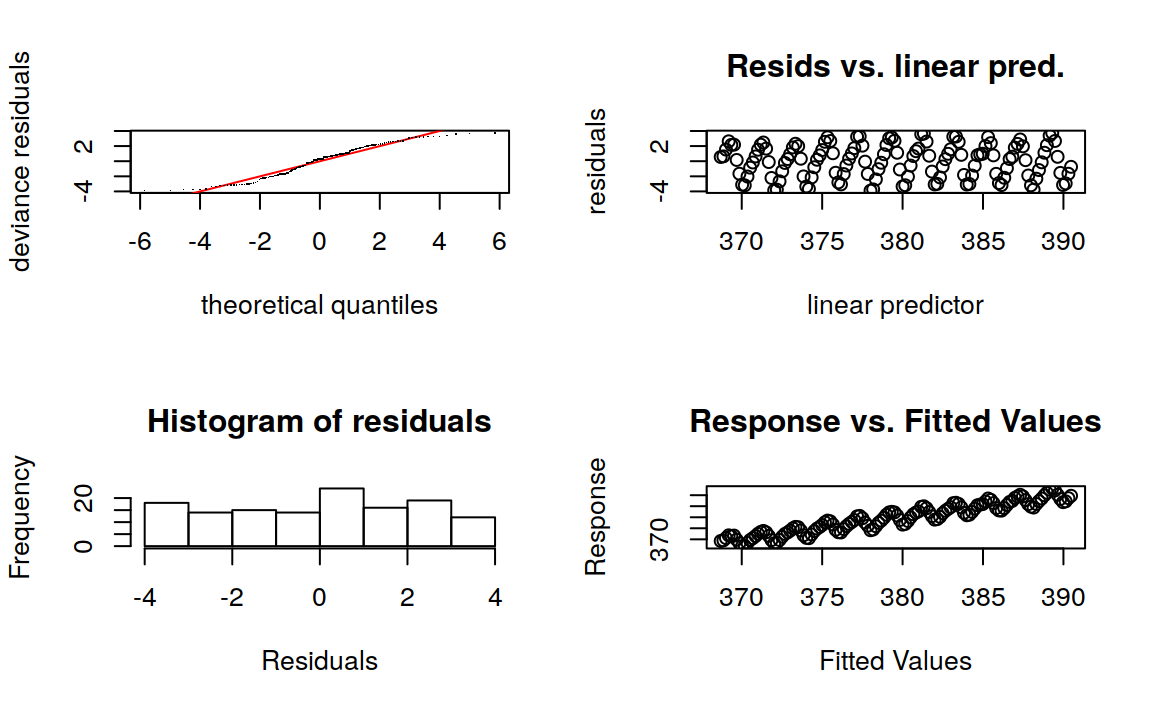
\includegraphics[width=0.7\linewidth]{meta_110a-PCA-prcomp_vs_princomp_files/figure-latex/unnamed-chunk-8-1} \end{center}

\begin{quote}
From the plot above, we might want to stop at the fifth principal component. 87\% of the information (variances) contained in the data are retained by the first five principal components.
\end{quote}

\hypertarget{plots-quality-and-contribution}{%
\section{Plots: quality and contribution}\label{plots-quality-and-contribution}}

\begin{enumerate}
\def\labelenumi{\arabic{enumi}.}
\setcounter{enumi}{3}
\tightlist
\item
  Graph of individuals. Individuals with a similar profile are grouped together.
\end{enumerate}

\begin{Shaded}
\begin{Highlighting}[]
\CommentTok{# Graph of individuals.}
\KeywordTok{fviz_pca_ind}\NormalTok{(res.pca,}
             \DataTypeTok{col.ind =} \StringTok{"cos2"}\NormalTok{, }\CommentTok{# Color by the quality of representation}
             \DataTypeTok{gradient.cols =} \KeywordTok{c}\NormalTok{(}\StringTok{"#00AFBB"}\NormalTok{, }\StringTok{"#E7B800"}\NormalTok{, }\StringTok{"#FC4E07"}\NormalTok{),}
             \DataTypeTok{repel =} \OtherTok{TRUE}     \CommentTok{# Avoid text overlapping}
\NormalTok{             )}
\end{Highlighting}
\end{Shaded}

\begin{center}\includegraphics[width=0.7\linewidth]{meta_110a-PCA-prcomp_vs_princomp_files/figure-latex/unnamed-chunk-9-1} \end{center}

\begin{enumerate}
\def\labelenumi{\arabic{enumi}.}
\setcounter{enumi}{4}
\tightlist
\item
  Graph of variables. Positive correlated variables point to the same side of the plot. Negative correlated variables point to opposite sides of the graph.
\end{enumerate}

\begin{Shaded}
\begin{Highlighting}[]
\CommentTok{# Graph of variables.}
\KeywordTok{fviz_pca_var}\NormalTok{(res.pca,}
             \DataTypeTok{col.var =} \StringTok{"contrib"}\NormalTok{, }\CommentTok{# Color by contributions to the PC}
             \DataTypeTok{gradient.cols =} \KeywordTok{c}\NormalTok{(}\StringTok{"#00AFBB"}\NormalTok{, }\StringTok{"#E7B800"}\NormalTok{, }\StringTok{"#FC4E07"}\NormalTok{),}
             \DataTypeTok{repel =} \OtherTok{TRUE}     \CommentTok{# Avoid text overlapping}
\NormalTok{             )}
\end{Highlighting}
\end{Shaded}

\begin{center}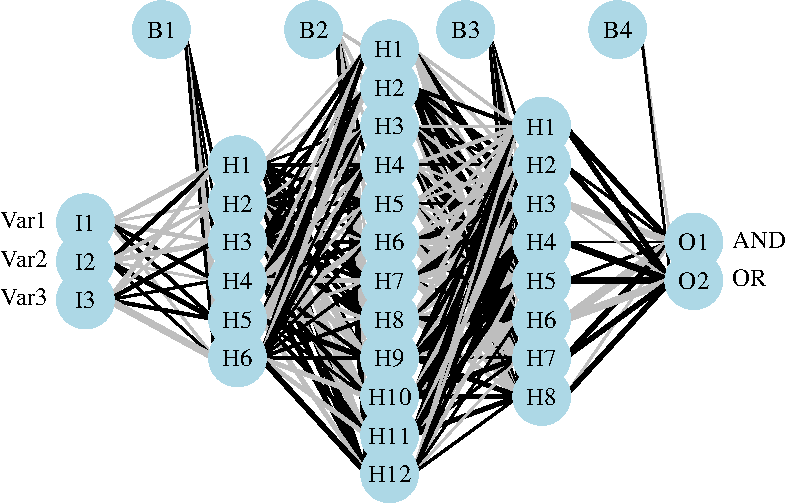
\includegraphics[width=0.7\linewidth]{meta_110a-PCA-prcomp_vs_princomp_files/figure-latex/unnamed-chunk-10-1} \end{center}

\begin{enumerate}
\def\labelenumi{\arabic{enumi}.}
\setcounter{enumi}{5}
\tightlist
\item
  Biplot of individuals and variables
\end{enumerate}

\begin{Shaded}
\begin{Highlighting}[]
\CommentTok{# Biplot of individuals and variables}
\KeywordTok{fviz_pca_biplot}\NormalTok{(res.pca, }\DataTypeTok{repel =} \OtherTok{TRUE}\NormalTok{,}
                \DataTypeTok{col.var =} \StringTok{"#2E9FDF"}\NormalTok{, }\CommentTok{# Variables color}
                \DataTypeTok{col.ind =} \StringTok{"#696969"}  \CommentTok{# Individuals color}
\NormalTok{                )}
\end{Highlighting}
\end{Shaded}

\begin{center}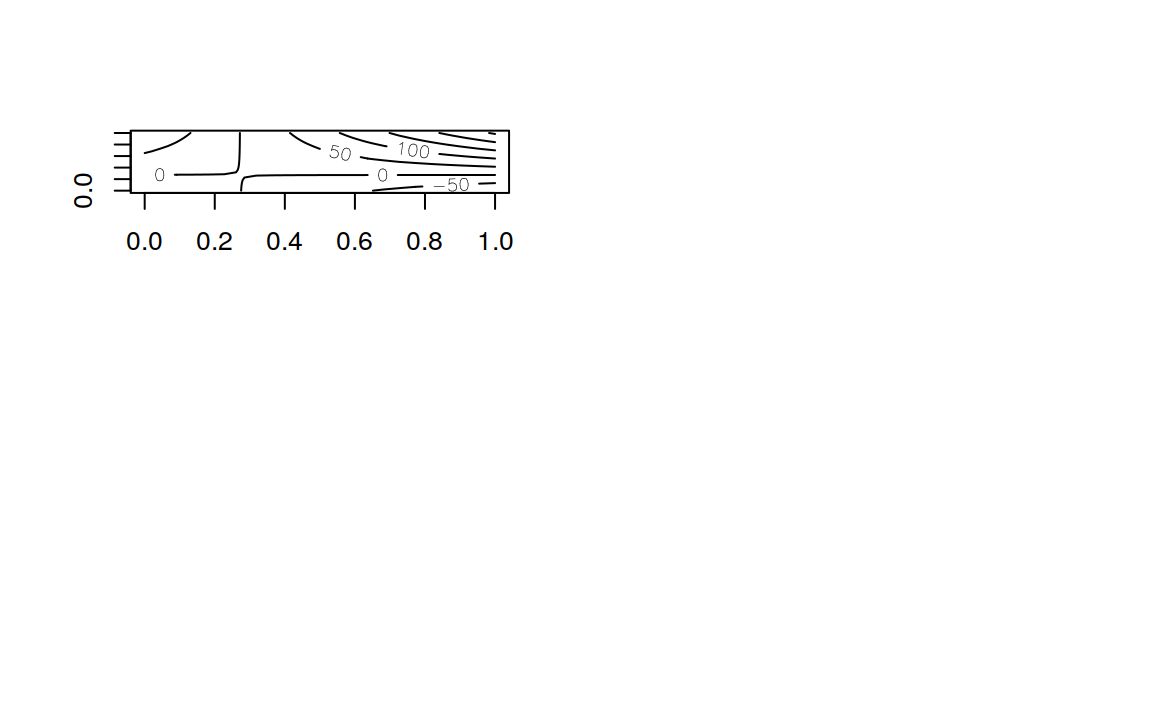
\includegraphics[width=0.7\linewidth]{meta_110a-PCA-prcomp_vs_princomp_files/figure-latex/unnamed-chunk-11-1} \end{center}

\hypertarget{access-to-the-pca-results}{%
\section{Access to the PCA results}\label{access-to-the-pca-results}}

\begin{Shaded}
\begin{Highlighting}[]
\KeywordTok{library}\NormalTok{(factoextra)}
\CommentTok{# Eigenvalues}
\NormalTok{eig.val <-}\StringTok{ }\KeywordTok{get_eigenvalue}\NormalTok{(res.pca)}
\NormalTok{eig.val}
\CommentTok{#>        eigenvalue variance.percent cumulative.variance.percent}
\CommentTok{#> Dim.1       4.124            41.24                        41.2}
\CommentTok{#> Dim.2       1.839            18.39                        59.6}
\CommentTok{#> Dim.3       1.239            12.39                        72.0}
\CommentTok{#> Dim.4       0.819             8.19                        80.2}
\CommentTok{#> Dim.5       0.702             7.02                        87.2}
\CommentTok{#> Dim.6       0.423             4.23                        91.5}
\CommentTok{#> Dim.7       0.303             3.03                        94.5}
\CommentTok{#> Dim.8       0.274             2.74                        97.2}
\CommentTok{#> Dim.9       0.155             1.55                        98.8}
\CommentTok{#> Dim.10      0.122             1.22                       100.0}
  
\CommentTok{# Results for Variables}
\NormalTok{res.var <-}\StringTok{ }\KeywordTok{get_pca_var}\NormalTok{(res.pca)}
\NormalTok{res.var}\OperatorTok{$}\NormalTok{coord          }\CommentTok{# Coordinates}
\CommentTok{#>                 Dim.1   Dim.2   Dim.3   Dim.4  Dim.5    Dim.6    Dim.7}
\CommentTok{#> X100m        -0.85063  0.1794 -0.3016  0.0336 -0.194  0.03537 -0.09134}
\CommentTok{#> Long.jump     0.79418 -0.2809  0.1905 -0.1154  0.233 -0.03373 -0.15433}
\CommentTok{#> Shot.put      0.73391 -0.0854 -0.5176  0.1285 -0.249 -0.23979 -0.00989}
\CommentTok{#> High.jump     0.61008  0.4652 -0.3301  0.1446  0.403 -0.28464  0.02816}
\CommentTok{#> X400m        -0.70160 -0.2902 -0.2835  0.4308  0.104 -0.04929  0.28611}
\CommentTok{#> X110m.hurdle -0.76413  0.0247 -0.4489 -0.0169  0.224  0.00263 -0.37007}
\CommentTok{#> Discus        0.74321 -0.0497 -0.1765  0.3950 -0.408  0.19854 -0.14273}
\CommentTok{#> Pole.vault   -0.21727 -0.8075 -0.0941 -0.3390 -0.222 -0.32746 -0.01039}
\CommentTok{#> Javeline      0.42823 -0.3861 -0.6041 -0.3317  0.198  0.36210  0.13356}
\CommentTok{#> X1500m        0.00428 -0.7845  0.2195  0.4480  0.263  0.04205 -0.11137}
\CommentTok{#>                 Dim.8   Dim.9   Dim.10}
\CommentTok{#> X100m        -0.10472 -0.3031  0.04442}
\CommentTok{#> Long.jump    -0.39738 -0.0516  0.02972}
\CommentTok{#> Shot.put      0.02436  0.0478  0.21745}
\CommentTok{#> High.jump     0.08441 -0.1121 -0.13357}
\CommentTok{#> X400m        -0.23355  0.0822 -0.03417}
\CommentTok{#> X110m.hurdle -0.00834  0.1618 -0.01563}
\CommentTok{#> Discus       -0.03956  0.0134 -0.17259}
\CommentTok{#> Pole.vault    0.03291 -0.0258 -0.13721}
\CommentTok{#> Javeline      0.05284 -0.0405 -0.00385}
\CommentTok{#> X1500m        0.19447 -0.1022  0.06283}
\NormalTok{res.var}\OperatorTok{$}\NormalTok{contrib        }\CommentTok{# Contributions to the PCs}
\CommentTok{#>                 Dim.1   Dim.2  Dim.3   Dim.4 Dim.5    Dim.6   Dim.7}
\CommentTok{#> X100m        1.75e+01  1.7505  7.339  0.1376  5.39  0.29592  2.7571}
\CommentTok{#> Long.jump    1.53e+01  4.2904  2.930  1.6249  7.75  0.26900  7.8716}
\CommentTok{#> Shot.put     1.31e+01  0.3967 21.620  2.0141  8.82 13.59686  0.0323}
\CommentTok{#> High.jump    9.02e+00 11.7716  8.793  2.5499 23.12 19.15961  0.2620}
\CommentTok{#> X400m        1.19e+01  4.5799  6.488 22.6509  1.54  0.57451 27.0527}
\CommentTok{#> X110m.hurdle 1.42e+01  0.0333 16.261  0.0348  7.17  0.00164 45.2616}
\CommentTok{#> Discus       1.34e+01  0.1341  2.515 19.0413 23.76  9.32175  6.7323}
\CommentTok{#> Pole.vault   1.14e+00 35.4619  0.714 14.0231  7.01 25.35762  0.0357}
\CommentTok{#> Javeline     4.45e+00  8.1087 29.453 13.4296  5.58 31.00496  5.8957}
\CommentTok{#> X1500m       4.44e-04 33.4729  3.887 24.4939  9.88  0.41813  4.0989}
\CommentTok{#>                Dim.8  Dim.9  Dim.10}
\CommentTok{#> X100m         3.9952 59.174  1.6176}
\CommentTok{#> Long.jump    57.5332  1.715  0.7241}
\CommentTok{#> Shot.put      0.2162  1.471 38.7677}
\CommentTok{#> High.jump     2.5957  8.102 14.6265}
\CommentTok{#> X400m        19.8734  4.349  0.9573}
\CommentTok{#> X110m.hurdle  0.0254 16.858  0.2003}
\CommentTok{#> Discus        0.5702  0.115 24.4217}
\CommentTok{#> Pole.vault    0.3947  0.428 15.4356}
\CommentTok{#> Javeline      1.0173  1.054  0.0122}
\CommentTok{#> X1500m       13.7787  6.734  3.2370}
\NormalTok{res.var}\OperatorTok{$}\NormalTok{cos2           }\CommentTok{# Quality of representation }
\CommentTok{#>                 Dim.1    Dim.2   Dim.3    Dim.4  Dim.5    Dim.6    Dim.7}
\CommentTok{#> X100m        7.24e-01 0.032184 0.09094 0.001127 0.0378 1.25e-03 8.34e-03}
\CommentTok{#> Long.jump    6.31e-01 0.078881 0.03631 0.013315 0.0544 1.14e-03 2.38e-02}
\CommentTok{#> Shot.put     5.39e-01 0.007294 0.26791 0.016504 0.0619 5.75e-02 9.77e-05}
\CommentTok{#> High.jump    3.72e-01 0.216424 0.10896 0.020895 0.1622 8.10e-02 7.93e-04}
\CommentTok{#> X400m        4.92e-01 0.084203 0.08039 0.185611 0.0108 2.43e-03 8.19e-02}
\CommentTok{#> X110m.hurdle 5.84e-01 0.000612 0.20150 0.000285 0.0503 6.93e-06 1.37e-01}
\CommentTok{#> Discus       5.52e-01 0.002466 0.03116 0.156032 0.1667 3.94e-02 2.04e-02}
\CommentTok{#> Pole.vault   4.72e-02 0.651977 0.00885 0.114911 0.0491 1.07e-01 1.08e-04}
\CommentTok{#> Javeline     1.83e-01 0.149080 0.36497 0.110048 0.0391 1.31e-01 1.78e-02}
\CommentTok{#> X1500m       1.83e-05 0.615409 0.04817 0.200713 0.0693 1.77e-03 1.24e-02}
\CommentTok{#>                 Dim.8    Dim.9   Dim.10}
\CommentTok{#> X100m        1.10e-02 0.091848 1.97e-03}
\CommentTok{#> Long.jump    1.58e-01 0.002661 8.83e-04}
\CommentTok{#> Shot.put     5.93e-04 0.002284 4.73e-02}
\CommentTok{#> High.jump    7.12e-03 0.012575 1.78e-02}
\CommentTok{#> X400m        5.45e-02 0.006750 1.17e-03}
\CommentTok{#> X110m.hurdle 6.96e-05 0.026166 2.44e-04}
\CommentTok{#> Discus       1.56e-03 0.000179 2.98e-02}
\CommentTok{#> Pole.vault   1.08e-03 0.000664 1.88e-02}
\CommentTok{#> Javeline     2.79e-03 0.001637 1.49e-05}
\CommentTok{#> X1500m       3.78e-02 0.010453 3.95e-03}
\CommentTok{# Results for individuals}
\NormalTok{res.ind <-}\StringTok{ }\KeywordTok{get_pca_ind}\NormalTok{(res.pca)}
\NormalTok{res.ind}\OperatorTok{$}\NormalTok{coord          }\CommentTok{# Coordinates}
\CommentTok{#>              Dim.1  Dim.2  Dim.3   Dim.4     Dim.5   Dim.6   Dim.7}
\CommentTok{#> SEBRLE       0.191 -1.554 -0.628  0.0821  1.142614 -0.4639 -0.2080}
\CommentTok{#> CLAY         0.790 -2.420  1.357  1.2698 -0.806848  1.3042 -0.2129}
\CommentTok{#> BERNARD     -1.329 -1.612 -0.196 -1.9209  0.082343 -0.4006 -0.4064}
\CommentTok{#> YURKOV      -0.869  0.433 -2.474  0.6972  0.398858  0.1029 -0.3249}
\CommentTok{#> ZSIVOCZKY   -0.106  2.023  1.305 -0.0993 -0.197024  0.8955  0.0883}
\CommentTok{#> McMULLEN     0.119  0.992  0.844  1.3122  1.585871  0.1866  0.4783}
\CommentTok{#> MARTINEAU   -2.392  1.285 -0.898  0.3731 -2.243352 -0.4567 -0.2998}
\CommentTok{#> HERNU       -1.891 -1.178 -0.156  0.8913 -0.126741  0.4362 -0.5661}
\CommentTok{#> BARRAS      -1.774  0.413  0.658  0.2287 -0.233837  0.0903  0.2159}
\CommentTok{#> NOOL        -2.777  1.573  0.607 -1.5555  1.424184  0.4972 -0.5321}
\CommentTok{#> BOURGUIGNON -4.414 -1.264 -0.010  0.6668  0.419152 -0.0820 -0.5983}
\CommentTok{#> Sebrle       3.451 -1.217 -1.678 -0.8087 -0.025053 -0.0828  0.0102}
\CommentTok{#> Clay         3.316 -1.623 -0.618 -0.3168  0.569165  0.7772  0.2575}
\CommentTok{#> Karpov       4.070  0.798  1.015  0.3134 -0.797426 -0.3296 -1.3637}
\CommentTok{#> Macey        1.848  2.064 -0.979  0.5847 -0.000216 -0.1973 -0.2693}
\CommentTok{#> Warners      1.387 -0.282  2.000 -1.0196 -0.040540 -0.5567 -0.2674}
\CommentTok{#> Zsivoczky    0.472  0.927 -1.728 -0.1848  0.407303 -0.1138  0.0399}
\CommentTok{#> Hernu        0.276  1.166  0.171 -0.8487 -0.689480 -0.3317  0.4431}
\CommentTok{#> Bernard      1.367  1.478  0.831  0.7453  0.859802 -0.3281  0.3636}
\CommentTok{#> Schwarzl    -0.710 -0.658  1.041 -0.9272 -0.288757 -0.6889  0.5657}
\CommentTok{#> Pogorelov   -0.214 -0.861  0.298  1.3556 -0.015053 -1.5938  0.7837}
\CommentTok{#> Schoenbeck  -0.495 -1.300  0.103 -0.2493 -0.645226  0.1617  0.8575}
\CommentTok{#> Barras      -0.316  0.819 -0.862 -0.5894 -0.779739  1.1742  0.9451}
\CommentTok{#>                Dim.8    Dim.9  Dim.10}
\CommentTok{#> SEBRLE       0.04346 -0.65934  0.0327}
\CommentTok{#> CLAY         0.61724 -0.06013 -0.3172}
\CommentTok{#> BERNARD      0.70386  0.17008 -0.0991}
\CommentTok{#> YURKOV       0.11500 -0.10952 -0.1197}
\CommentTok{#> ZSIVOCZKY   -0.20234 -0.52310 -0.3484}
\CommentTok{#> McMULLEN     0.29309 -0.10562 -0.3932}
\CommentTok{#> MARTINEAU   -0.29163 -0.22342 -0.6164}
\CommentTok{#> HERNU       -1.52940  0.00618  0.5537}
\CommentTok{#> BARRAS       0.68258 -0.66928  0.5309}
\CommentTok{#> NOOL        -0.43339 -0.11578 -0.0962}
\CommentTok{#> BOURGUIGNON  0.56362  0.52581  0.0586}
\CommentTok{#> Sebrle      -0.03059 -0.84721  0.2197}
\CommentTok{#> Clay        -0.58064  0.40978 -0.6160}
\CommentTok{#> Karpov       0.34531  0.19306  0.2172}
\CommentTok{#> Macey       -0.36322  0.36826  0.2125}
\CommentTok{#> Warners     -0.10947  0.18028  0.2421}
\CommentTok{#> Zsivoczky    0.53804  0.58597 -0.1427}
\CommentTok{#> Hernu        0.24729  0.06691 -0.2087}
\CommentTok{#> Bernard      0.00617  0.27949  0.3207}
\CommentTok{#> Schwarzl    -0.68705 -0.00836 -0.3021}
\CommentTok{#> Pogorelov   -0.03762 -0.13053 -0.0370}
\CommentTok{#> Schoenbeck  -0.25585  0.56422  0.2968}
\CommentTok{#> Barras       0.36555  0.10226  0.6119}
\NormalTok{res.ind}\OperatorTok{$}\NormalTok{contrib        }\CommentTok{# Contributions to the PCs}
\CommentTok{#>               Dim.1  Dim.2    Dim.3   Dim.4    Dim.5   Dim.6    Dim.7}
\CommentTok{#> SEBRLE       0.0385  5.712 1.39e+00  0.0357 8.09e+00  2.2126  0.62143}
\CommentTok{#> CLAY         0.6581 13.854 6.46e+00  8.5557 4.03e+00 17.4880  0.65141}
\CommentTok{#> BERNARD      1.8627  6.144 1.35e-01 19.5783 4.20e-02  1.6502  2.37365}
\CommentTok{#> YURKOV       0.7969  0.443 2.15e+01  2.5794 9.86e-01  0.1088  1.51656}
\CommentTok{#> ZSIVOCZKY    0.0118  9.682 5.97e+00  0.0523 2.41e-01  8.2456  0.11192}
\CommentTok{#> McMULLEN     0.0148  2.325 2.50e+00  9.1353 1.56e+01  0.3579  3.28702}
\CommentTok{#> MARTINEAU    6.0337  3.904 2.83e+00  0.7386 3.12e+01  2.1441  1.29111}
\CommentTok{#> HERNU        3.7700  3.284 8.58e-02  4.2151 9.96e-02  1.9566  4.60485}
\CommentTok{#> BARRAS       3.3194  0.402 1.52e+00  0.2776 3.39e-01  0.0838  0.67004}
\CommentTok{#> NOOL         8.1299  5.849 1.29e+00 12.8376 1.26e+01  2.5413  4.06767}
\CommentTok{#> BOURGUIGNON 20.5373  3.776 3.53e-04  2.3588 1.09e+00  0.0691  5.14425}
\CommentTok{#> Sebrle      12.5584  3.502 9.88e+00  3.4701 3.89e-03  0.0705  0.00148}
\CommentTok{#> Clay        11.5936  6.232 1.34e+00  0.5325 2.01e+00  6.2097  0.95282}
\CommentTok{#> Karpov      17.4661  1.507 3.61e+00  0.5210 3.94e+00  1.1168 26.72016}
\CommentTok{#> Macey        3.6021 10.073 3.36e+00  1.8139 2.89e-07  0.4001  1.04191}
\CommentTok{#> Warners      2.0291  0.188 1.40e+01  5.5159 1.02e-02  3.1867  1.02738}
\CommentTok{#> Zsivoczky    0.2344  2.031 1.05e+01  0.1813 1.03e+00  0.1332  0.02289}
\CommentTok{#> Hernu        0.0805  3.214 1.02e-01  3.8217 2.95e+00  1.1311  2.82103}
\CommentTok{#> Bernard      1.9708  5.166 2.43e+00  2.9474 4.58e+00  1.1066  1.89945}
\CommentTok{#> Schwarzl     0.5318  1.025 3.80e+00  4.5612 5.17e-01  4.8796  4.59812}
\CommentTok{#> Pogorelov    0.0484  1.753 3.11e-01  9.7503 1.40e-03 26.1167  8.82532}
\CommentTok{#> Schoenbeck   0.2586  3.997 3.72e-02  0.3297 2.58e+00  0.2689 10.56627}
\CommentTok{#> Barras       0.1052  1.588 2.61e+00  1.8430 3.77e+00 14.1743 12.83542}
\CommentTok{#>                Dim.8    Dim.9  Dim.10}
\CommentTok{#> SEBRLE      2.99e-02 12.17748  0.0382}
\CommentTok{#> CLAY        6.04e+00  0.10126  3.5857}
\CommentTok{#> BERNARD     7.85e+00  0.81032  0.3499}
\CommentTok{#> YURKOV      2.09e-01  0.33601  0.5107}
\CommentTok{#> ZSIVOCZKY   6.49e-01  7.66492  4.3274}
\CommentTok{#> McMULLEN    1.36e+00  0.31250  5.5105}
\CommentTok{#> MARTINEAU   1.35e+00  1.39820 13.5440}
\CommentTok{#> HERNU       3.71e+01  0.00107 10.9278}
\CommentTok{#> BARRAS      7.38e+00 12.54733 10.0454}
\CommentTok{#> NOOL        2.98e+00  0.37548  0.3300}
\CommentTok{#> BOURGUIGNON 5.03e+00  7.74457  0.1222}
\CommentTok{#> Sebrle      1.48e-02 20.10555  1.7206}
\CommentTok{#> Clay        5.34e+00  4.70357 13.5271}
\CommentTok{#> Karpov      1.89e+00  1.04399  1.6819}
\CommentTok{#> Macey       2.09e+00  3.79877  1.6096}
\CommentTok{#> Warners     1.90e-01  0.91042  2.0890}
\CommentTok{#> Zsivoczky   4.59e+00  9.61785  0.7261}
\CommentTok{#> Hernu       9.69e-01  0.12540  1.5523}
\CommentTok{#> Bernard     6.02e-04  2.18807  3.6657}
\CommentTok{#> Schwarzl    7.48e+00  0.00196  3.2536}
\CommentTok{#> Pogorelov   2.24e-02  0.47727  0.0487}
\CommentTok{#> Schoenbeck  1.04e+00  8.91730  3.1402}
\CommentTok{#> Barras      2.12e+00  0.29289 13.3453}
\NormalTok{res.ind}\OperatorTok{$}\NormalTok{cos2           }\CommentTok{# Quality of representation }
\CommentTok{#>               Dim.1  Dim.2    Dim.3   Dim.4    Dim.5    Dim.6    Dim.7}
\CommentTok{#> SEBRLE      0.00753 0.4975 8.13e-02 0.00139 2.69e-01 0.044324 8.91e-03}
\CommentTok{#> CLAY        0.04870 0.4570 1.44e-01 0.12579 5.08e-02 0.132691 3.54e-03}
\CommentTok{#> BERNARD     0.19720 0.2900 4.29e-03 0.41182 7.57e-04 0.017913 1.84e-02}
\CommentTok{#> YURKOV      0.09611 0.0238 7.78e-01 0.06181 2.02e-02 0.001345 1.34e-02}
\CommentTok{#> ZSIVOCZKY   0.00157 0.5764 2.40e-01 0.00139 5.47e-03 0.112918 1.10e-03}
\CommentTok{#> McMULLEN    0.00218 0.1522 1.10e-01 0.26649 3.89e-01 0.005388 3.54e-02}
\CommentTok{#> MARTINEAU   0.40401 0.1165 5.69e-02 0.00983 3.55e-01 0.014721 6.34e-03}
\CommentTok{#> HERNU       0.39928 0.1551 2.73e-03 0.08870 1.79e-03 0.021248 3.58e-02}
\CommentTok{#> BARRAS      0.61624 0.0333 8.48e-02 0.01024 1.07e-02 0.001594 9.13e-03}
\CommentTok{#> NOOL        0.48987 0.1571 2.34e-02 0.15369 1.29e-01 0.015701 1.80e-02}
\CommentTok{#> BOURGUIGNON 0.85970 0.0705 4.45e-06 0.01962 7.75e-03 0.000297 1.58e-02}
\CommentTok{#> Sebrle      0.67538 0.0840 1.60e-01 0.03708 3.56e-05 0.000389 5.85e-06}
\CommentTok{#> Clay        0.68759 0.1648 2.39e-02 0.00627 2.03e-02 0.037763 4.15e-03}
\CommentTok{#> Karpov      0.78367 0.0301 4.87e-02 0.00464 3.01e-02 0.005138 8.80e-02}
\CommentTok{#> Macey       0.36344 0.4531 1.02e-01 0.03636 4.95e-09 0.004140 7.71e-03}
\CommentTok{#> Warners     0.25565 0.0106 5.31e-01 0.13808 2.18e-04 0.041169 9.50e-03}
\CommentTok{#> Zsivoczky   0.04505 0.1740 6.05e-01 0.00692 3.36e-02 0.002625 3.23e-04}
\CommentTok{#> Hernu       0.02482 0.4418 9.46e-03 0.23420 1.55e-01 0.035771 6.38e-02}
\CommentTok{#> Bernard     0.28935 0.3381 1.07e-01 0.08598 1.14e-01 0.016659 2.05e-02}
\CommentTok{#> Schwarzl    0.11672 0.1003 2.51e-01 0.19889 1.93e-02 0.109806 7.40e-02}
\CommentTok{#> Pogorelov   0.00780 0.1259 1.50e-02 0.31210 3.85e-05 0.431416 1.04e-01}
\CommentTok{#> Schoenbeck  0.06707 0.4620 2.90e-03 0.01699 1.14e-01 0.007150 2.01e-01}
\CommentTok{#> Barras      0.01897 0.1277 1.41e-01 0.06604 1.16e-01 0.262130 1.70e-01}
\CommentTok{#>                Dim.8    Dim.9   Dim.10}
\CommentTok{#> SEBRLE      3.89e-04 8.95e-02 0.000221}
\CommentTok{#> CLAY        2.97e-02 2.82e-04 0.007847}
\CommentTok{#> BERNARD     5.53e-02 3.23e-03 0.001096}
\CommentTok{#> YURKOV      1.68e-03 1.53e-03 0.001822}
\CommentTok{#> ZSIVOCZKY   5.76e-03 3.85e-02 0.017092}
\CommentTok{#> McMULLEN    1.33e-02 1.73e-03 0.023927}
\CommentTok{#> MARTINEAU   6.00e-03 3.52e-03 0.026821}
\CommentTok{#> HERNU       2.61e-01 4.27e-06 0.034229}
\CommentTok{#> BARRAS      9.12e-02 8.77e-02 0.055153}
\CommentTok{#> NOOL        1.19e-02 8.51e-04 0.000588}
\CommentTok{#> BOURGUIGNON 1.40e-02 1.22e-02 0.000151}
\CommentTok{#> Sebrle      5.30e-05 4.07e-02 0.002737}
\CommentTok{#> Clay        2.11e-02 1.05e-02 0.023726}
\CommentTok{#> Karpov      5.64e-03 1.76e-03 0.002232}
\CommentTok{#> Macey       1.40e-02 1.44e-02 0.004803}
\CommentTok{#> Warners     1.59e-03 4.32e-03 0.007784}
\CommentTok{#> Zsivoczky   5.87e-02 6.96e-02 0.004127}
\CommentTok{#> Hernu       1.99e-02 1.46e-03 0.014160}
\CommentTok{#> Bernard     5.88e-06 1.21e-02 0.015917}
\CommentTok{#> Schwarzl    1.09e-01 1.62e-05 0.021117}
\CommentTok{#> Pogorelov   2.40e-04 2.89e-03 0.000232}
\CommentTok{#> Schoenbeck  1.79e-02 8.70e-02 0.024083}
\CommentTok{#> Barras      2.54e-02 1.99e-03 0.071184}
\end{Highlighting}
\end{Shaded}

\hypertarget{predict-using-pca}{%
\section{Predict using PCA}\label{predict-using-pca}}

In this section, we'll show how to predict the coordinates of supplementary individuals and variables using only the information provided by the previously performed PCA.

\begin{enumerate}
\def\labelenumi{\arabic{enumi}.}
\tightlist
\item
  Data: rows 24 to 27 and columns 1 to to 10 {[}in decathlon2 data sets{]}. The new data must contain columns (variables) with the same names and in the same order as the active data used to compute PCA.
\end{enumerate}

\begin{Shaded}
\begin{Highlighting}[]
\CommentTok{# Data for the supplementary individuals}
\NormalTok{ind.sup <-}\StringTok{ }\NormalTok{decathlon2[}\DecValTok{24}\OperatorTok{:}\DecValTok{27}\NormalTok{, }\DecValTok{1}\OperatorTok{:}\DecValTok{10}\NormalTok{]}
\NormalTok{ind.sup[, }\DecValTok{1}\OperatorTok{:}\DecValTok{6}\NormalTok{]}
\CommentTok{#>         X100m Long.jump Shot.put High.jump X400m X110m.hurdle}
\CommentTok{#> KARPOV   11.0      7.30     14.8      2.04  48.4         14.1}
\CommentTok{#> WARNERS  11.1      7.60     14.3      1.98  48.7         14.2}
\CommentTok{#> Nool     10.8      7.53     14.3      1.88  48.8         14.8}
\CommentTok{#> Drews    10.9      7.38     13.1      1.88  48.5         14.0}
\end{Highlighting}
\end{Shaded}

\begin{enumerate}
\def\labelenumi{\arabic{enumi}.}
\setcounter{enumi}{1}
\tightlist
\item
  Predict the coordinates of new individuals data. Use the R base function predict():
\end{enumerate}

\begin{Shaded}
\begin{Highlighting}[]
\NormalTok{ind.sup.coord <-}\StringTok{ }\KeywordTok{predict}\NormalTok{(res.pca, }\DataTypeTok{newdata =}\NormalTok{ ind.sup)}
\NormalTok{ind.sup.coord[, }\DecValTok{1}\OperatorTok{:}\DecValTok{4}\NormalTok{]}
\CommentTok{#>            PC1    PC2   PC3    PC4}
\CommentTok{#> KARPOV   0.777 -0.762 1.597  1.686}
\CommentTok{#> WARNERS -0.378  0.119 1.701 -0.691}
\CommentTok{#> Nool    -0.547 -1.934 0.472 -2.228}
\CommentTok{#> Drews   -1.085 -0.017 2.982 -1.501}
\end{Highlighting}
\end{Shaded}

\begin{enumerate}
\def\labelenumi{\arabic{enumi}.}
\setcounter{enumi}{2}
\tightlist
\item
  Graph of individuals including the supplementary individuals:
\end{enumerate}

\begin{Shaded}
\begin{Highlighting}[]
\CommentTok{# Plot of active individuals}
\NormalTok{p <-}\StringTok{ }\KeywordTok{fviz_pca_ind}\NormalTok{(res.pca, }\DataTypeTok{repel =} \OtherTok{TRUE}\NormalTok{)}
\CommentTok{# Add supplementary individuals}
\KeywordTok{fviz_add}\NormalTok{(p, ind.sup.coord, }\DataTypeTok{color =}\StringTok{"blue"}\NormalTok{)}
\end{Highlighting}
\end{Shaded}

\begin{center}\includegraphics[width=0.7\linewidth]{meta_110a-PCA-prcomp_vs_princomp_files/figure-latex/unnamed-chunk-15-1} \end{center}

The predicted coordinates of individuals can be manually calculated as follow:

\begin{enumerate}
\def\labelenumi{\arabic{enumi}.}
\tightlist
\item
  Center and scale the new individuals data using the center and the scale of the PCA
\item
  Calculate the predicted coordinates by multiplying the scaled values with the eigenvectors (loadings) of the principal components.
  The R code below can be used :
\end{enumerate}

\begin{Shaded}
\begin{Highlighting}[]
\CommentTok{# Centering and scaling the supplementary individuals}
\NormalTok{ind.scaled <-}\StringTok{ }\KeywordTok{scale}\NormalTok{(ind.sup, }
                    \DataTypeTok{center =}\NormalTok{ res.pca}\OperatorTok{$}\NormalTok{center,}
                    \DataTypeTok{scale =}\NormalTok{ res.pca}\OperatorTok{$}\NormalTok{scale)}
\CommentTok{# Coordinates of the individividuals}
\NormalTok{coord_func <-}\StringTok{ }\ControlFlowTok{function}\NormalTok{(ind, loadings)\{}
\NormalTok{  r <-}\StringTok{ }\NormalTok{loadings}\OperatorTok{*}\NormalTok{ind}
  \KeywordTok{apply}\NormalTok{(r, }\DecValTok{2}\NormalTok{, sum)}
\NormalTok{\}}
\NormalTok{pca.loadings <-}\StringTok{ }\NormalTok{res.pca}\OperatorTok{$}\NormalTok{rotation}
\NormalTok{ind.sup.coord <-}\StringTok{ }\KeywordTok{t}\NormalTok{(}\KeywordTok{apply}\NormalTok{(ind.scaled, }\DecValTok{1}\NormalTok{, coord_func, pca.loadings ))}
\NormalTok{ind.sup.coord[, }\DecValTok{1}\OperatorTok{:}\DecValTok{4}\NormalTok{]}
\CommentTok{#>            PC1    PC2   PC3    PC4}
\CommentTok{#> KARPOV   0.777 -0.762 1.597  1.686}
\CommentTok{#> WARNERS -0.378  0.119 1.701 -0.691}
\CommentTok{#> Nool    -0.547 -1.934 0.472 -2.228}
\CommentTok{#> Drews   -1.085 -0.017 2.982 -1.501}
\end{Highlighting}
\end{Shaded}

\hypertarget{supplementary-variables}{%
\section{Supplementary variables}\label{supplementary-variables}}

\hypertarget{qualitative-categorical-variables}{%
\subsection{Qualitative / categorical variables}\label{qualitative-categorical-variables}}

The data sets decathlon2 contain a supplementary qualitative variable at columns 13 corresponding to the type of competitions.

Qualitative / categorical variables can be used to color individuals by groups. The grouping variable should be of same length as the number of active individuals (here 23).

\begin{Shaded}
\begin{Highlighting}[]
\NormalTok{groups <-}\StringTok{ }\KeywordTok{as.factor}\NormalTok{(decathlon2}\OperatorTok{$}\NormalTok{Competition[}\DecValTok{1}\OperatorTok{:}\DecValTok{23}\NormalTok{])}
\KeywordTok{fviz_pca_ind}\NormalTok{(res.pca,}
             \DataTypeTok{col.ind =}\NormalTok{ groups, }\CommentTok{# color by groups}
             \DataTypeTok{palette =} \KeywordTok{c}\NormalTok{(}\StringTok{"#00AFBB"}\NormalTok{,  }\StringTok{"#FC4E07"}\NormalTok{),}
             \DataTypeTok{addEllipses =} \OtherTok{TRUE}\NormalTok{, }\CommentTok{# Concentration ellipses}
             \DataTypeTok{ellipse.type =} \StringTok{"confidence"}\NormalTok{,}
             \DataTypeTok{legend.title =} \StringTok{"Groups"}\NormalTok{,}
             \DataTypeTok{repel =} \OtherTok{TRUE}
\NormalTok{             )}
\end{Highlighting}
\end{Shaded}

\begin{center}\includegraphics[width=0.7\linewidth]{meta_110a-PCA-prcomp_vs_princomp_files/figure-latex/unnamed-chunk-17-1} \end{center}

Calculate the coordinates for the levels of grouping variables. The coordinates for a given group is calculated as the mean coordinates of the individuals in the group.

\begin{Shaded}
\begin{Highlighting}[]
\KeywordTok{library}\NormalTok{(magrittr) }\CommentTok{# for pipe %>%}
\KeywordTok{library}\NormalTok{(dplyr)   }\CommentTok{# everything else}
\CommentTok{#> }
\CommentTok{#> Attaching package: 'dplyr'}
\CommentTok{#> The following objects are masked from 'package:stats':}
\CommentTok{#> }
\CommentTok{#>     filter, lag}
\CommentTok{#> The following objects are masked from 'package:base':}
\CommentTok{#> }
\CommentTok{#>     intersect, setdiff, setequal, union}

\CommentTok{# 1. Individual coordinates}
\NormalTok{res.ind <-}\StringTok{ }\KeywordTok{get_pca_ind}\NormalTok{(res.pca)}
\CommentTok{# 2. Coordinate of groups}
\NormalTok{coord.groups <-}\StringTok{ }\NormalTok{res.ind}\OperatorTok{$}\NormalTok{coord }\OperatorTok
\StringTok{  }\KeywordTok{as_data_frame}\NormalTok{() }\OperatorTok
\StringTok{  }\KeywordTok{select}\NormalTok{(Dim}\FloatTok{.1}\NormalTok{, Dim}\FloatTok{.2}\NormalTok{) }\OperatorTok
\StringTok{  }\KeywordTok{mutate}\NormalTok{(}\DataTypeTok{competition =}\NormalTok{ groups) }\OperatorTok
\StringTok{  }\KeywordTok{group_by}\NormalTok{(competition) }\OperatorTok
\StringTok{  }\KeywordTok{summarise}\NormalTok{(}
    \DataTypeTok{Dim.1 =} \KeywordTok{mean}\NormalTok{(Dim}\FloatTok{.1}\NormalTok{),}
    \DataTypeTok{Dim.2 =} \KeywordTok{mean}\NormalTok{(Dim}\FloatTok{.2}\NormalTok{)}
\NormalTok{    )}
\CommentTok{#> Warning: `as_data_frame()` is deprecated, use `as_tibble()` (but mind the new semantics).}
\CommentTok{#> This warning is displayed once per session.}
\NormalTok{coord.groups}
\CommentTok{#> # A tibble: 2 x 3}
\CommentTok{#>   competition Dim.1  Dim.2}
\CommentTok{#>   <fct>       <dbl>  <dbl>}
\CommentTok{#> 1 Decastar    -1.31 -0.119}
\CommentTok{#> 2 OlympicG     1.20  0.109}
\end{Highlighting}
\end{Shaded}

\hypertarget{quantitative-variables}{%
\subsection{Quantitative variables}\label{quantitative-variables}}

Data: columns 11:12. Should be of same length as the number of active individuals (here 23)

\begin{Shaded}
\begin{Highlighting}[]
\NormalTok{quanti.sup <-}\StringTok{ }\NormalTok{decathlon2[}\DecValTok{1}\OperatorTok{:}\DecValTok{23}\NormalTok{, }\DecValTok{11}\OperatorTok{:}\DecValTok{12}\NormalTok{, drop =}\StringTok{ }\OtherTok{FALSE}\NormalTok{]}
\KeywordTok{head}\NormalTok{(quanti.sup)}
\CommentTok{#>           Rank Points}
\CommentTok{#> SEBRLE       1   8217}
\CommentTok{#> CLAY         2   8122}
\CommentTok{#> BERNARD      4   8067}
\CommentTok{#> YURKOV       5   8036}
\CommentTok{#> ZSIVOCZKY    7   8004}
\CommentTok{#> McMULLEN     8   7995}
\end{Highlighting}
\end{Shaded}

The coordinates of a given quantitative variable are calculated as the correlation between the quantitative variables and the principal components.

\begin{Shaded}
\begin{Highlighting}[]
\CommentTok{# Predict coordinates and compute cos2}
\NormalTok{quanti.coord <-}\StringTok{ }\KeywordTok{cor}\NormalTok{(quanti.sup, res.pca}\OperatorTok{$}\NormalTok{x)}
\NormalTok{quanti.cos2 <-}\StringTok{ }\NormalTok{quanti.coord}\OperatorTok{^}\DecValTok{2}
\CommentTok{# Graph of variables including supplementary variables}
\NormalTok{p <-}\StringTok{ }\KeywordTok{fviz_pca_var}\NormalTok{(res.pca)}
\KeywordTok{fviz_add}\NormalTok{(p, quanti.coord, }\DataTypeTok{color =}\StringTok{"blue"}\NormalTok{, }\DataTypeTok{geom=}\StringTok{"arrow"}\NormalTok{)}
\end{Highlighting}
\end{Shaded}

\begin{center}\includegraphics[width=0.7\linewidth]{meta_110a-PCA-prcomp_vs_princomp_files/figure-latex/unnamed-chunk-20-1} \end{center}

\hypertarget{theory-behind-pca-results}{%
\section{Theory behind PCA results}\label{theory-behind-pca-results}}

\hypertarget{pca-results-for-variables}{%
\subsection{PCA results for variables}\label{pca-results-for-variables}}

Here we'll show how to calculate the PCA results for variables: coordinates, cos2 and contributions:

\texttt{var.coord} = loadings * the component standard deviations
\texttt{var.cos2} = var.coord\^{}2
\texttt{var.contrib}. The contribution of a variable to a given principal component is (in percentage) : (var.cos2 * 100) / (total cos2 of the component)

\begin{Shaded}
\begin{Highlighting}[]
\CommentTok{# Helper function }
\CommentTok{#::::::::::::::::::::::::::::::::::::::::}
\NormalTok{var_coord_func <-}\StringTok{ }\ControlFlowTok{function}\NormalTok{(loadings, comp.sdev)\{}
\NormalTok{  loadings}\OperatorTok{*}\NormalTok{comp.sdev}
\NormalTok{\}}
\end{Highlighting}
\end{Shaded}

\begin{Shaded}
\begin{Highlighting}[]
\CommentTok{# Compute Coordinates}
\CommentTok{#::::::::::::::::::::::::::::::::::::::::}
\NormalTok{loadings <-}\StringTok{ }\NormalTok{res.pca}\OperatorTok{$}\NormalTok{rotation}
\NormalTok{sdev <-}\StringTok{ }\NormalTok{res.pca}\OperatorTok{$}\NormalTok{sdev}
\NormalTok{var.coord <-}\StringTok{ }\KeywordTok{t}\NormalTok{(}\KeywordTok{apply}\NormalTok{(loadings, }\DecValTok{1}\NormalTok{, var_coord_func, sdev)) }
\KeywordTok{head}\NormalTok{(var.coord[, }\DecValTok{1}\OperatorTok{:}\DecValTok{4}\NormalTok{])}
\CommentTok{#>                 PC1     PC2    PC3     PC4}
\CommentTok{#> X100m        -0.851  0.1794 -0.302  0.0336}
\CommentTok{#> Long.jump     0.794 -0.2809  0.191 -0.1154}
\CommentTok{#> Shot.put      0.734 -0.0854 -0.518  0.1285}
\CommentTok{#> High.jump     0.610  0.4652 -0.330  0.1446}
\CommentTok{#> X400m        -0.702 -0.2902 -0.284  0.4308}
\CommentTok{#> X110m.hurdle -0.764  0.0247 -0.449 -0.0169}
\end{Highlighting}
\end{Shaded}

\begin{Shaded}
\begin{Highlighting}[]
\CommentTok{# Compute Cos2}
\CommentTok{#::::::::::::::::::::::::::::::::::::::::}
\NormalTok{var.cos2 <-}\StringTok{ }\NormalTok{var.coord}\OperatorTok{^}\DecValTok{2}
\KeywordTok{head}\NormalTok{(var.cos2[, }\DecValTok{1}\OperatorTok{:}\DecValTok{4}\NormalTok{])}
\CommentTok{#>                PC1      PC2    PC3      PC4}
\CommentTok{#> X100m        0.724 0.032184 0.0909 0.001127}
\CommentTok{#> Long.jump    0.631 0.078881 0.0363 0.013315}
\CommentTok{#> Shot.put     0.539 0.007294 0.2679 0.016504}
\CommentTok{#> High.jump    0.372 0.216424 0.1090 0.020895}
\CommentTok{#> X400m        0.492 0.084203 0.0804 0.185611}
\CommentTok{#> X110m.hurdle 0.584 0.000612 0.2015 0.000285}
\end{Highlighting}
\end{Shaded}

\begin{Shaded}
\begin{Highlighting}[]
\CommentTok{# Compute contributions}
\CommentTok{#::::::::::::::::::::::::::::::::::::::::}
\NormalTok{comp.cos2 <-}\StringTok{ }\KeywordTok{apply}\NormalTok{(var.cos2, }\DecValTok{2}\NormalTok{, sum)}
\NormalTok{contrib <-}\StringTok{ }\ControlFlowTok{function}\NormalTok{(var.cos2, comp.cos2)\{var.cos2}\OperatorTok{*}\DecValTok{100}\OperatorTok{/}\NormalTok{comp.cos2\}}
\NormalTok{var.contrib <-}\StringTok{ }\KeywordTok{t}\NormalTok{(}\KeywordTok{apply}\NormalTok{(var.cos2,}\DecValTok{1}\NormalTok{, contrib, comp.cos2))}
\KeywordTok{head}\NormalTok{(var.contrib[, }\DecValTok{1}\OperatorTok{:}\DecValTok{4}\NormalTok{])}
\CommentTok{#>                PC1     PC2   PC3     PC4}
\CommentTok{#> X100m        17.54  1.7505  7.34  0.1376}
\CommentTok{#> Long.jump    15.29  4.2904  2.93  1.6249}
\CommentTok{#> Shot.put     13.06  0.3967 21.62  2.0141}
\CommentTok{#> High.jump     9.02 11.7716  8.79  2.5499}
\CommentTok{#> X400m        11.94  4.5799  6.49 22.6509}
\CommentTok{#> X110m.hurdle 14.16  0.0333 16.26  0.0348}
\end{Highlighting}
\end{Shaded}

\hypertarget{pca-results-for-individuals}{%
\subsection{PCA results for individuals}\label{pca-results-for-individuals}}

\begin{itemize}
\tightlist
\item
  \texttt{ind.coord} = res.pca\$x
\item
  Cos2 of individuals. Two steps:

  \begin{itemize}
  \tightlist
  \item
    Calculate the square distance between each individual and the PCA center of gravity: d2 = {[}(var1\_ind\_i - mean\_var1)/sd\_var1{]}\^{}2 + \ldots{}+ {[}(var10\_ind\_i - mean\_var10)/sd\_var10{]}\^{}2 + \ldots{}+..
  \item
    Calculate the cos2 as ind.coord\^{}2/d2
  \end{itemize}
\item
  Contributions of individuals to the principal components: 100 * (1 / number\_of\_individuals)*(ind.coord\^{}2 / comp\_sdev\^{}2). Note that the sum of all the contributions per column is 100
\end{itemize}

\begin{Shaded}
\begin{Highlighting}[]
\CommentTok{# Coordinates of individuals}
\CommentTok{#::::::::::::::::::::::::::::::::::}
\NormalTok{ind.coord <-}\StringTok{ }\NormalTok{res.pca}\OperatorTok{$}\NormalTok{x}
\KeywordTok{head}\NormalTok{(ind.coord[, }\DecValTok{1}\OperatorTok{:}\DecValTok{4}\NormalTok{])}
\CommentTok{#>              PC1    PC2    PC3     PC4}
\CommentTok{#> SEBRLE     0.191 -1.554 -0.628  0.0821}
\CommentTok{#> CLAY       0.790 -2.420  1.357  1.2698}
\CommentTok{#> BERNARD   -1.329 -1.612 -0.196 -1.9209}
\CommentTok{#> YURKOV    -0.869  0.433 -2.474  0.6972}
\CommentTok{#> ZSIVOCZKY -0.106  2.023  1.305 -0.0993}
\CommentTok{#> McMULLEN   0.119  0.992  0.844  1.3122}
\end{Highlighting}
\end{Shaded}

\begin{Shaded}
\begin{Highlighting}[]
\CommentTok{# Cos2 of individuals}
\CommentTok{#:::::::::::::::::::::::::::::::::}
\CommentTok{# 1. square of the distance between an individual and the}
\CommentTok{# PCA center of gravity}
\NormalTok{center <-}\StringTok{ }\NormalTok{res.pca}\OperatorTok{$}\NormalTok{center}
\NormalTok{scale<-}\StringTok{ }\NormalTok{res.pca}\OperatorTok{$}\NormalTok{scale}

\NormalTok{getdistance <-}\StringTok{ }\ControlFlowTok{function}\NormalTok{(ind_row, center, scale)\{}
  \KeywordTok{return}\NormalTok{(}\KeywordTok{sum}\NormalTok{(((ind_row}\OperatorTok{-}\NormalTok{center)}\OperatorTok{/}\NormalTok{scale)}\OperatorTok{^}\DecValTok{2}\NormalTok{))}
\NormalTok{\}}

\NormalTok{d2 <-}\StringTok{ }\KeywordTok{apply}\NormalTok{(decathlon2.active,}\DecValTok{1}\NormalTok{, getdistance, center, scale)}
\CommentTok{# 2. Compute the cos2. The sum of each row is 1}
\NormalTok{cos2 <-}\StringTok{ }\ControlFlowTok{function}\NormalTok{(ind.coord, d2)\{}\KeywordTok{return}\NormalTok{(ind.coord}\OperatorTok{^}\DecValTok{2}\OperatorTok{/}\NormalTok{d2)\}}
\NormalTok{ind.cos2 <-}\StringTok{ }\KeywordTok{apply}\NormalTok{(ind.coord, }\DecValTok{2}\NormalTok{, cos2, d2)}
\KeywordTok{head}\NormalTok{(ind.cos2[, }\DecValTok{1}\OperatorTok{:}\DecValTok{4}\NormalTok{])}
\CommentTok{#>               PC1    PC2     PC3     PC4}
\CommentTok{#> SEBRLE    0.00753 0.4975 0.08133 0.00139}
\CommentTok{#> CLAY      0.04870 0.4570 0.14363 0.12579}
\CommentTok{#> BERNARD   0.19720 0.2900 0.00429 0.41182}
\CommentTok{#> YURKOV    0.09611 0.0238 0.77823 0.06181}
\CommentTok{#> ZSIVOCZKY 0.00157 0.5764 0.23975 0.00139}
\CommentTok{#> McMULLEN  0.00218 0.1522 0.11014 0.26649}
\end{Highlighting}
\end{Shaded}

\begin{Shaded}
\begin{Highlighting}[]
\CommentTok{# Contributions of individuals}
\CommentTok{#:::::::::::::::::::::::::::::::}
\NormalTok{contrib <-}\StringTok{ }\ControlFlowTok{function}\NormalTok{(ind.coord, comp.sdev, n.ind)\{}
  \DecValTok{100}\OperatorTok{*}\NormalTok{(}\DecValTok{1}\OperatorTok{/}\NormalTok{n.ind)}\OperatorTok{*}\NormalTok{ind.coord}\OperatorTok{^}\DecValTok{2}\OperatorTok{/}\NormalTok{comp.sdev}\OperatorTok{^}\DecValTok{2}
\NormalTok{\}}
\NormalTok{ind.contrib <-}\StringTok{ }\KeywordTok{t}\NormalTok{(}\KeywordTok{apply}\NormalTok{(ind.coord, }\DecValTok{1}\NormalTok{, contrib, }
\NormalTok{                       res.pca}\OperatorTok{$}\NormalTok{sdev, }\KeywordTok{nrow}\NormalTok{(ind.coord)))}
\KeywordTok{head}\NormalTok{(ind.contrib[, }\DecValTok{1}\OperatorTok{:}\DecValTok{4}\NormalTok{])}
\CommentTok{#>              PC1    PC2    PC3     PC4}
\CommentTok{#> SEBRLE    0.0385  5.712  1.385  0.0357}
\CommentTok{#> CLAY      0.6581 13.854  6.460  8.5557}
\CommentTok{#> BERNARD   1.8627  6.144  0.135 19.5783}
\CommentTok{#> YURKOV    0.7969  0.443 21.476  2.5794}
\CommentTok{#> ZSIVOCZKY 0.0118  9.682  5.975  0.0523}
\CommentTok{#> McMULLEN  0.0148  2.325  2.497  9.1353}
\end{Highlighting}
\end{Shaded}

\hypertarget{principal-components-methods}{%
\chapter{Principal Components Methods}\label{principal-components-methods}}

\url{http://www.sthda.com/english/articles/31-principal-component-methods-in-r-practical-guide/112-pca-principal-component-analysis-essentials/}

Principal component analysis (PCA) allows us to summarize and to visualize the information in a data set containing individuals/observations described by multiple inter-correlated quantitative variables. Each variable could be considered as a different dimension. If you have more than 3 variables in your data sets, it could be very difficult to visualize a multi-dimensional hyperspace.

Principal component analysis is used to extract the important information from a multivariate data table and to express this information as a set of few new variables called principal components. These new variables correspond to a linear combination of the originals. The number of principal components is less than or equal to the number of original variables.

The information in a given data set corresponds to the total variation it contains. The goal of PCA is to identify directions (or principal components) along which the variation in the data is maximal.

In other words, PCA reduces the dimensionality of a multivariate data to two or three principal components, that can be visualized graphically, with minimal loss of information.

\begin{Shaded}
\begin{Highlighting}[]
\CommentTok{# install.packages(c("FactoMineR", "factoextra"))}
\end{Highlighting}
\end{Shaded}

\begin{Shaded}
\begin{Highlighting}[]
\KeywordTok{library}\NormalTok{(FactoMineR)}
\KeywordTok{library}\NormalTok{(factoextra)}
\CommentTok{#> Loading required package: ggplot2}
\CommentTok{#> Registered S3 methods overwritten by 'ggplot2':}
\CommentTok{#>   method         from }
\CommentTok{#>   [.quosures     rlang}
\CommentTok{#>   c.quosures     rlang}
\CommentTok{#>   print.quosures rlang}
\CommentTok{#> Welcome! Related Books: `Practical Guide To Cluster Analysis in R` at https://goo.gl/13EFCZ}
\end{Highlighting}
\end{Shaded}

\begin{Shaded}
\begin{Highlighting}[]
\KeywordTok{data}\NormalTok{(decathlon2)}
\CommentTok{# head(decathlon2)}
\end{Highlighting}
\end{Shaded}

In PCA terminology, our data contains :

\begin{itemize}
\item
  Active individuals (in light blue, rows 1:23) : Individuals that are used during the principal component analysis.
\item
  Supplementary individuals (in dark blue, rows 24:27) : The coordinates of these individuals will be predicted using the PCA information and parameters obtained with active individuals/variables
\item
  Active variables (in pink, columns 1:10) : Variables that are used for the principal component analysis.
\item
  Supplementary variables: As supplementary individuals, the coordinates of these variables will be predicted also. These can be:

  \begin{itemize}
  \tightlist
  \item
    Supplementary continuous variables (red): Columns 11 and 12 corresponding respectively to the rank and the points of athletes.
  \item
    Supplementary qualitative variables (green): Column 13 corresponding to the two athlete-tic meetings (2004 Olympic Game or 2004 Decastar). This is a categorical (or factor) variable factor. It can be used to color individuals by groups.
  \end{itemize}
\end{itemize}

We start by subsetting active individuals and active variables for the principal component analysis:

\begin{Shaded}
\begin{Highlighting}[]
\NormalTok{decathlon2.active <-}\StringTok{ }\NormalTok{decathlon2[}\DecValTok{1}\OperatorTok{:}\DecValTok{23}\NormalTok{, }\DecValTok{1}\OperatorTok{:}\DecValTok{10}\NormalTok{]}
\KeywordTok{head}\NormalTok{(decathlon2.active[, }\DecValTok{1}\OperatorTok{:}\DecValTok{6}\NormalTok{], }\DecValTok{4}\NormalTok{)}
\CommentTok{#>         X100m Long.jump Shot.put High.jump X400m X110m.hurdle}
\CommentTok{#> SEBRLE   11.0      7.58     14.8      2.07  49.8         14.7}
\CommentTok{#> CLAY     10.8      7.40     14.3      1.86  49.4         14.1}
\CommentTok{#> BERNARD  11.0      7.23     14.2      1.92  48.9         15.0}
\CommentTok{#> YURKOV   11.3      7.09     15.2      2.10  50.4         15.3}
\end{Highlighting}
\end{Shaded}

\hypertarget{data-standardization}{%
\section{Data standardization}\label{data-standardization}}

In principal component analysis, variables are often scaled (i.e.~standardized). This is particularly recommended when variables are measured in different scales (e.g: kilograms, kilometers, centimeters, \ldots{}); otherwise, the PCA outputs obtained will be severely affected.

The goal is to make the variables comparable. Generally variables are scaled to have i) standard deviation one and ii) mean zero.

The function PCA() {[}FactoMineR package{]} can be used. A simplified format is:

\begin{Shaded}
\begin{Highlighting}[]
\KeywordTok{library}\NormalTok{(FactoMineR)}
\NormalTok{res.pca <-}\StringTok{ }\KeywordTok{PCA}\NormalTok{(decathlon2.active, }\DataTypeTok{graph =} \OtherTok{FALSE}\NormalTok{)}
\end{Highlighting}
\end{Shaded}

\begin{Shaded}
\begin{Highlighting}[]
\KeywordTok{print}\NormalTok{(res.pca)}
\CommentTok{#> **Results for the Principal Component Analysis (PCA)**}
\CommentTok{#> The analysis was performed on 23 individuals, described by 10 variables}
\CommentTok{#> *The results are available in the following objects:}
\CommentTok{#> }
\CommentTok{#>    name               description                          }
\CommentTok{#> 1  "$eig"             "eigenvalues"                        }
\CommentTok{#> 2  "$var"             "results for the variables"          }
\CommentTok{#> 3  "$var$coord"       "coord. for the variables"           }
\CommentTok{#> 4  "$var$cor"         "correlations variables - dimensions"}
\CommentTok{#> 5  "$var$cos2"        "cos2 for the variables"             }
\CommentTok{#> 6  "$var$contrib"     "contributions of the variables"     }
\CommentTok{#> 7  "$ind"             "results for the individuals"        }
\CommentTok{#> 8  "$ind$coord"       "coord. for the individuals"         }
\CommentTok{#> 9  "$ind$cos2"        "cos2 for the individuals"           }
\CommentTok{#> 10 "$ind$contrib"     "contributions of the individuals"   }
\CommentTok{#> 11 "$call"            "summary statistics"                 }
\CommentTok{#> 12 "$call$centre"     "mean of the variables"              }
\CommentTok{#> 13 "$call$ecart.type" "standard error of the variables"    }
\CommentTok{#> 14 "$call$row.w"      "weights for the individuals"        }
\CommentTok{#> 15 "$call$col.w"      "weights for the variables"}
\end{Highlighting}
\end{Shaded}

\begin{quote}
The object that is created using the function PCA() contains many information found in many different lists and matrices. These values are described in the next section.
\end{quote}

\hypertarget{eigenvalues-variances}{%
\section{Eigenvalues / Variances}\label{eigenvalues-variances}}

As described in previous sections, the eigenvalues measure the amount of variation retained by each principal component. Eigenvalues are large for the first PCs and small for the subsequent PCs. That is, the first PCs corresponds to the directions with the maximum amount of variation in the data set.

We examine the eigenvalues to determine the number of principal components to be considered. The eigenvalues and the proportion of variances (i.e., information) retained by the principal components (PCs) can be extracted using the function get\_eigenvalue() {[}factoextra package{]}.

\begin{Shaded}
\begin{Highlighting}[]
\KeywordTok{library}\NormalTok{(factoextra)}
\NormalTok{eig.val <-}\StringTok{ }\KeywordTok{get_eigenvalue}\NormalTok{(res.pca)}
\NormalTok{eig.val}
\CommentTok{#>        eigenvalue variance.percent cumulative.variance.percent}
\CommentTok{#> Dim.1       4.124            41.24                        41.2}
\CommentTok{#> Dim.2       1.839            18.39                        59.6}
\CommentTok{#> Dim.3       1.239            12.39                        72.0}
\CommentTok{#> Dim.4       0.819             8.19                        80.2}
\CommentTok{#> Dim.5       0.702             7.02                        87.2}
\CommentTok{#> Dim.6       0.423             4.23                        91.5}
\CommentTok{#> Dim.7       0.303             3.03                        94.5}
\CommentTok{#> Dim.8       0.274             2.74                        97.2}
\CommentTok{#> Dim.9       0.155             1.55                        98.8}
\CommentTok{#> Dim.10      0.122             1.22                       100.0}
\end{Highlighting}
\end{Shaded}

The sum of all the eigenvalues give a total variance of 10.

The proportion of variation explained by each eigenvalue is given in the second column. For example, 4.124 divided by 10 equals 0.4124, or, about 41.24\% of the variation is explained by this first eigenvalue. The cumulative percentage explained is obtained by adding the successive proportions of variation explained to obtain the running total. For instance, 41.242\% plus 18.385\% equals 59.627\%, and so forth. Therefore, about 59.627\% of the variation is explained by the first two eigenvalues together.

Unfortunately, there is no well-accepted objective way to decide how many principal components are enough. This will depend on the specific field of application and the specific data set. In practice, we tend to look at the first few principal components in order to find interesting patterns in the data.

In our analysis, the first three principal components explain 72\% of the variation. This is an acceptably large percentage.

An alternative method to determine the number of principal components is to look at a Scree Plot, which is the plot of eigenvalues ordered from largest to the smallest. The number of component is determined at the point, beyond which the remaining eigenvalues are all relatively small and of comparable size (Jollife 2002, Peres-Neto, Jackson, and Somers (2005)).

The scree plot can be produced using the function fviz\_eig() or fviz\_screeplot() {[}factoextra package{]}.

\begin{Shaded}
\begin{Highlighting}[]
\KeywordTok{fviz_eig}\NormalTok{(res.pca, }\DataTypeTok{addlabels =} \OtherTok{TRUE}\NormalTok{, }\DataTypeTok{ylim =} \KeywordTok{c}\NormalTok{(}\DecValTok{0}\NormalTok{, }\DecValTok{50}\NormalTok{))}
\end{Highlighting}
\end{Shaded}

\begin{center}\includegraphics[width=0.7\linewidth]{meta_110b-PCA-Principal_Component_Methods_in_R_files/figure-latex/unnamed-chunk-9-1} \end{center}

From the plot above, we might want to stop at the fifth principal component. 87\% of the information (variances) contained in the data are retained by the first five principal components.

\hypertarget{graph-of-variables}{%
\section{Graph of variables}\label{graph-of-variables}}

Results
A simple method to extract the results, for variables, from a PCA output is to use the function get\_pca\_var() {[}factoextra package{]}. This function provides a list of matrices containing all the results for the active variables (coordinates, correlation between variables and axes, squared cosine and contributions)

\begin{Shaded}
\begin{Highlighting}[]
\NormalTok{var <-}\StringTok{ }\KeywordTok{get_pca_var}\NormalTok{(res.pca)}
\NormalTok{var}
\CommentTok{#> Principal Component Analysis Results for variables}
\CommentTok{#>  ===================================================}
\CommentTok{#>   Name       Description                                    }
\CommentTok{#> 1 "$coord"   "Coordinates for the variables"                }
\CommentTok{#> 2 "$cor"     "Correlations between variables and dimensions"}
\CommentTok{#> 3 "$cos2"    "Cos2 for the variables"                       }
\CommentTok{#> 4 "$contrib" "contributions of the variables"}
\end{Highlighting}
\end{Shaded}

The components of the get\_pca\_var() can be used in the plot of variables as follow:

\begin{itemize}
\tightlist
\item
  var\$coord: coordinates of variables to create a scatter plot
\item
  var\$cos2: represents the quality of representation for variables on the factor map. It's calculated as the squared coordinates: var.cos2 = var.coord * var.coord.
\item
  var\$contrib: contains the contributions (in percentage) of the variables to the principal components. The contribution of a variable (var) to a given principal component is (in percentage) : (var.cos2 * 100) / (total cos2 of the component).
\end{itemize}

\begin{quote}
Note that, it's possible to plot variables and to color them according to either i) their quality on the factor map (cos2) or ii) their contribution values to the principal components (contrib).
\end{quote}

The different components can be accessed as follow:

\begin{Shaded}
\begin{Highlighting}[]
\CommentTok{# Coordinates}
\KeywordTok{head}\NormalTok{(var}\OperatorTok{$}\NormalTok{coord)}
\CommentTok{#>               Dim.1   Dim.2  Dim.3   Dim.4  Dim.5}
\CommentTok{#> X100m        -0.851 -0.1794  0.302  0.0336 -0.194}
\CommentTok{#> Long.jump     0.794  0.2809 -0.191 -0.1154  0.233}
\CommentTok{#> Shot.put      0.734  0.0854  0.518  0.1285 -0.249}
\CommentTok{#> High.jump     0.610 -0.4652  0.330  0.1446  0.403}
\CommentTok{#> X400m        -0.702  0.2902  0.284  0.4308  0.104}
\CommentTok{#> X110m.hurdle -0.764 -0.0247  0.449 -0.0169  0.224}
\CommentTok{# Cos2: quality on the factore map}
\KeywordTok{head}\NormalTok{(var}\OperatorTok{$}\NormalTok{cos2)}
\CommentTok{#>              Dim.1    Dim.2  Dim.3    Dim.4  Dim.5}
\CommentTok{#> X100m        0.724 0.032184 0.0909 0.001127 0.0378}
\CommentTok{#> Long.jump    0.631 0.078881 0.0363 0.013315 0.0544}
\CommentTok{#> Shot.put     0.539 0.007294 0.2679 0.016504 0.0619}
\CommentTok{#> High.jump    0.372 0.216424 0.1090 0.020895 0.1622}
\CommentTok{#> X400m        0.492 0.084203 0.0804 0.185611 0.0108}
\CommentTok{#> X110m.hurdle 0.584 0.000612 0.2015 0.000285 0.0503}
\CommentTok{# Contributions to the principal components}
\KeywordTok{head}\NormalTok{(var}\OperatorTok{$}\NormalTok{contrib)}
\CommentTok{#>              Dim.1   Dim.2 Dim.3   Dim.4 Dim.5}
\CommentTok{#> X100m        17.54  1.7505  7.34  0.1376  5.39}
\CommentTok{#> Long.jump    15.29  4.2904  2.93  1.6249  7.75}
\CommentTok{#> Shot.put     13.06  0.3967 21.62  2.0141  8.82}
\CommentTok{#> High.jump     9.02 11.7716  8.79  2.5499 23.12}
\CommentTok{#> X400m        11.94  4.5799  6.49 22.6509  1.54}
\CommentTok{#> X110m.hurdle 14.16  0.0333 16.26  0.0348  7.17}
\end{Highlighting}
\end{Shaded}

In this section, we describe how to visualize variables and draw conclusions about their correlations. Next, we highlight variables according to either i) their quality of representation on the factor map or ii) their contributions to the principal components.

\hypertarget{correlation-circle}{%
\section{Correlation circle}\label{correlation-circle}}

The correlation between a variable and a principal component (PC) is used as the coordinates of the variable on the PC. The representation of variables differs from the plot of the observations: The observations are represented by their projections, but the variables are represented by their correlations (Abdi and Williams 2010).

\begin{Shaded}
\begin{Highlighting}[]
\CommentTok{# Coordinates of variables}
\KeywordTok{head}\NormalTok{(var}\OperatorTok{$}\NormalTok{coord, }\DecValTok{4}\NormalTok{)}
\CommentTok{#>            Dim.1   Dim.2  Dim.3   Dim.4  Dim.5}
\CommentTok{#> X100m     -0.851 -0.1794  0.302  0.0336 -0.194}
\CommentTok{#> Long.jump  0.794  0.2809 -0.191 -0.1154  0.233}
\CommentTok{#> Shot.put   0.734  0.0854  0.518  0.1285 -0.249}
\CommentTok{#> High.jump  0.610 -0.4652  0.330  0.1446  0.403}
\end{Highlighting}
\end{Shaded}

To plot variables, type this:

\begin{Shaded}
\begin{Highlighting}[]
\KeywordTok{fviz_pca_var}\NormalTok{(res.pca, }\DataTypeTok{col.var =} \StringTok{"black"}\NormalTok{)}
\end{Highlighting}
\end{Shaded}

\begin{center}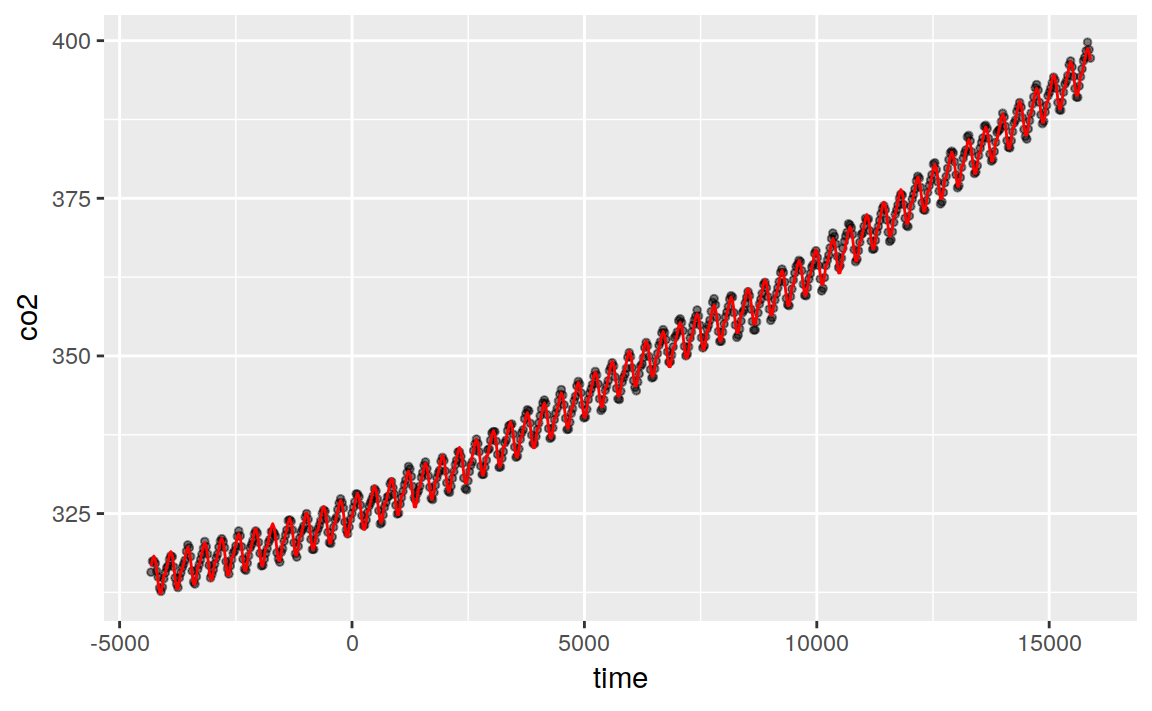
\includegraphics[width=0.7\linewidth]{meta_110b-PCA-Principal_Component_Methods_in_R_files/figure-latex/unnamed-chunk-13-1} \end{center}

The plot above is also known as variable correlation plots. It shows the relationships between all variables. It can be interpreted as follow:

\begin{itemize}
\tightlist
\item
  Positively correlated variables are grouped together.
\item
  Negatively correlated variables are positioned on opposite sides of the plot origin (opposed quadrants).
\item
  The distance between variables and the origin measures the quality of the variables on the factor map. Variables that are away from the origin are well represented on the factor map.
\end{itemize}

\hypertarget{quality-of-representation}{%
\section{Quality of representation}\label{quality-of-representation}}

The quality of representation of the variables on factor map is called cos2 (square cosine, squared coordinates) . You can access to the cos2 as follow:

\begin{Shaded}
\begin{Highlighting}[]
\KeywordTok{head}\NormalTok{(var}\OperatorTok{$}\NormalTok{cos2, }\DecValTok{4}\NormalTok{)}
\CommentTok{#>           Dim.1   Dim.2  Dim.3   Dim.4  Dim.5}
\CommentTok{#> X100m     0.724 0.03218 0.0909 0.00113 0.0378}
\CommentTok{#> Long.jump 0.631 0.07888 0.0363 0.01331 0.0544}
\CommentTok{#> Shot.put  0.539 0.00729 0.2679 0.01650 0.0619}
\CommentTok{#> High.jump 0.372 0.21642 0.1090 0.02089 0.1622}
\end{Highlighting}
\end{Shaded}

You can visualize the cos2 of variables on all the dimensions using the corrplot package:

\begin{Shaded}
\begin{Highlighting}[]
\KeywordTok{library}\NormalTok{(corrplot)}
\CommentTok{#> corrplot 0.84 loaded}
\KeywordTok{corrplot}\NormalTok{(var}\OperatorTok{$}\NormalTok{cos2, }\DataTypeTok{is.corr=}\OtherTok{FALSE}\NormalTok{)}
\end{Highlighting}
\end{Shaded}

\begin{center}\includegraphics[width=0.7\linewidth]{meta_110b-PCA-Principal_Component_Methods_in_R_files/figure-latex/unnamed-chunk-15-1} \end{center}

It's also possible to create a bar plot of variables cos2 using the function \texttt{fviz\_cos2()} {[}in factoextra{]}:

\begin{Shaded}
\begin{Highlighting}[]
\CommentTok{# Total cos2 of variables on Dim.1 and Dim.2}
\KeywordTok{fviz_cos2}\NormalTok{(res.pca, }\DataTypeTok{choice =} \StringTok{"var"}\NormalTok{, }\DataTypeTok{axes =} \DecValTok{1}\OperatorTok{:}\DecValTok{2}\NormalTok{)}
\end{Highlighting}
\end{Shaded}

\begin{center}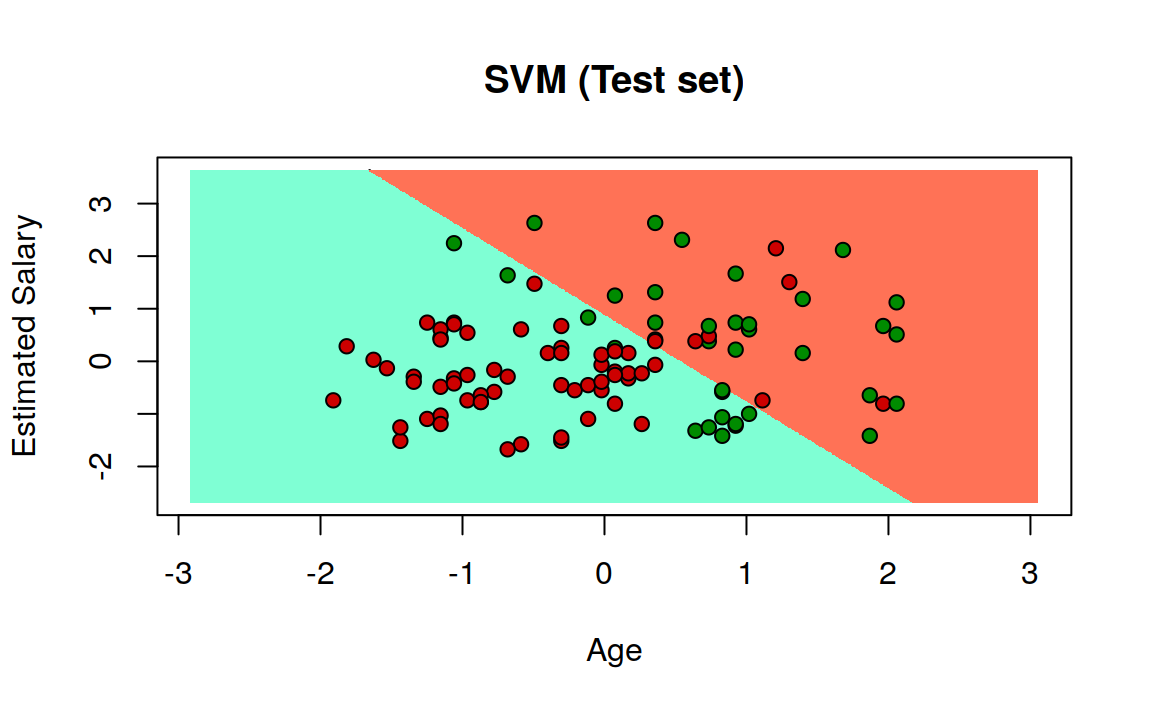
\includegraphics[width=0.7\linewidth]{meta_110b-PCA-Principal_Component_Methods_in_R_files/figure-latex/unnamed-chunk-16-1} \end{center}

Note that,

\begin{itemize}
\item
  A high cos2 indicates a good representation of the variable on the principal component. In this case the variable is positioned close to the circumference of the correlation circle.
\item
  A low cos2 indicates that the variable is not perfectly represented by the PCs. In this case the variable is close to the center of the circle.
\end{itemize}

For a given variable, the sum of the cos2 on all the principal components is equal to one.

If a variable is perfectly represented by only two principal components (Dim.1 \& Dim.2), the sum of the cos2 on these two PCs is equal to one. In this case the variables will be positioned on the circle of correlations.

For some of the variables, more than 2 components might be required to perfectly represent the data. In this case the variables are positioned inside the circle of correlations.

In summary:

\begin{itemize}
\tightlist
\item
  The cos2 values are used to estimate the quality of the representation
\item
  The closer a variable is to the circle of correlations, the better its representation on the factor map (and the more important it is to interpret these components)
\item
  Variables that are closed to the center of the plot are less important for the first components.
\end{itemize}

It's possible to color variables by their cos2 values using the argument col.var = ``cos2''. This produces a gradient colors. In this case, the argument gradient.cols can be used to provide a custom color. For instance, gradient.cols = c(``white'', ``blue'', ``red'') means that:

\begin{itemize}
\tightlist
\item
  variables with low cos2 values will be colored in ``white''
\item
  variables with mid cos2 values will be colored in ``blue''
\item
  variables with high cos2 values will be colored in red
\end{itemize}

\begin{Shaded}
\begin{Highlighting}[]
\CommentTok{# Color by cos2 values: quality on the factor map}
\KeywordTok{fviz_pca_var}\NormalTok{(res.pca, }\DataTypeTok{col.var =} \StringTok{"cos2"}\NormalTok{,}
             \DataTypeTok{gradient.cols =} \KeywordTok{c}\NormalTok{(}\StringTok{"#00AFBB"}\NormalTok{, }\StringTok{"#E7B800"}\NormalTok{, }\StringTok{"#FC4E07"}\NormalTok{), }
             \DataTypeTok{repel =} \OtherTok{TRUE} \CommentTok{# Avoid text overlapping}
\NormalTok{             )}
\end{Highlighting}
\end{Shaded}

\begin{center}\includegraphics[width=0.7\linewidth]{meta_110b-PCA-Principal_Component_Methods_in_R_files/figure-latex/unnamed-chunk-17-1} \end{center}

Note that, it's also possible to change the transparency of the variables according to their cos2 values using the option alpha.var = ``cos2''. For example, type this:

\begin{Shaded}
\begin{Highlighting}[]
\CommentTok{# Change the transparency by cos2 values}
\KeywordTok{fviz_pca_var}\NormalTok{(res.pca, }\DataTypeTok{alpha.var =} \StringTok{"cos2"}\NormalTok{)}
\end{Highlighting}
\end{Shaded}

\begin{center}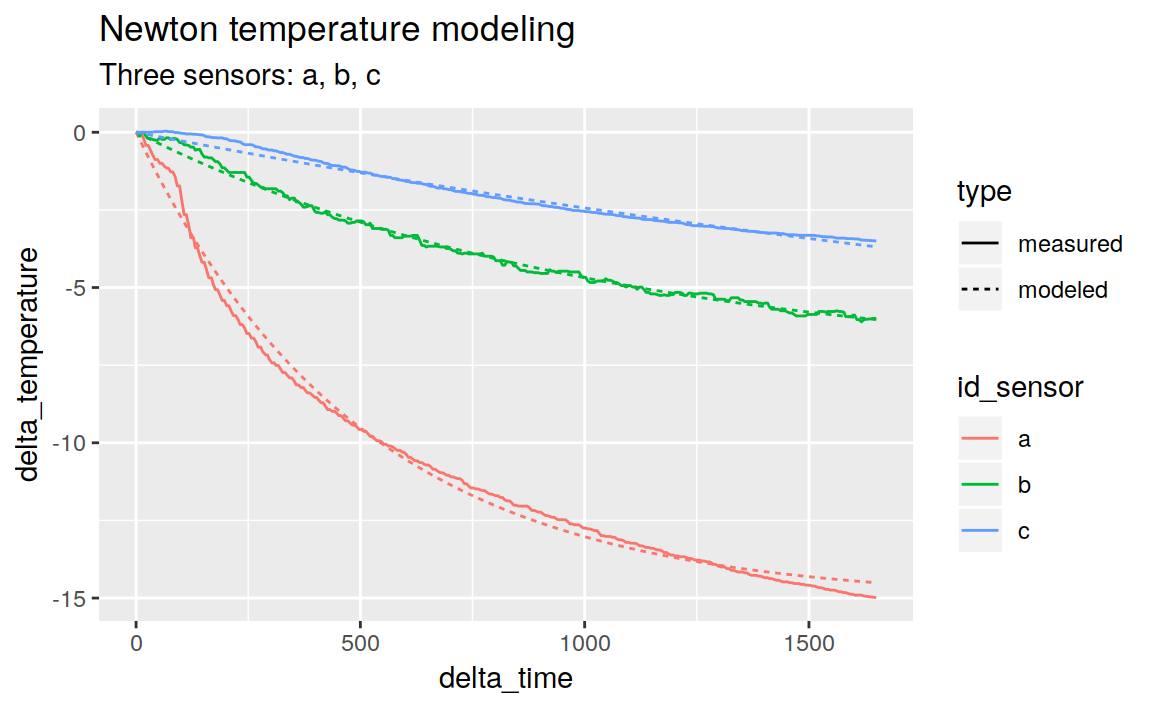
\includegraphics[width=0.7\linewidth]{meta_110b-PCA-Principal_Component_Methods_in_R_files/figure-latex/unnamed-chunk-18-1} \end{center}

\hypertarget{contributions-of-variables-to-pcs}{%
\section{Contributions of variables to PCs}\label{contributions-of-variables-to-pcs}}

The contributions of variables in accounting for the variability in a given principal component are expressed in percentage.

\begin{itemize}
\tightlist
\item
  Variables that are correlated with PC1 (i.e., Dim.1) and PC2 (i.e., Dim.2) are the most important in explaining the variability in the data set.
\item
  Variables that do not correlated with any PC or correlated with the last dimensions are variables with low contribution and might be removed to simplify the overall analysis.
\end{itemize}

The contribution of variables can be extracted as follow :

\begin{Shaded}
\begin{Highlighting}[]
\KeywordTok{head}\NormalTok{(var}\OperatorTok{$}\NormalTok{contrib, }\DecValTok{4}\NormalTok{)}
\CommentTok{#>           Dim.1  Dim.2 Dim.3 Dim.4 Dim.5}
\CommentTok{#> X100m     17.54  1.751  7.34 0.138  5.39}
\CommentTok{#> Long.jump 15.29  4.290  2.93 1.625  7.75}
\CommentTok{#> Shot.put  13.06  0.397 21.62 2.014  8.82}
\CommentTok{#> High.jump  9.02 11.772  8.79 2.550 23.12}
\end{Highlighting}
\end{Shaded}

\begin{quote}
The larger the value of the contribution, the more the variable contributes to the component.
\end{quote}

It's possible to use the function corrplot() {[}corrplot package{]} to highlight the most contributing variables for each dimension:

\begin{Shaded}
\begin{Highlighting}[]
\KeywordTok{library}\NormalTok{(}\StringTok{"corrplot"}\NormalTok{)}

\KeywordTok{corrplot}\NormalTok{(var}\OperatorTok{$}\NormalTok{contrib, }\DataTypeTok{is.corr=}\OtherTok{FALSE}\NormalTok{)    }
\end{Highlighting}
\end{Shaded}

\begin{center}\includegraphics[width=0.7\linewidth]{meta_110b-PCA-Principal_Component_Methods_in_R_files/figure-latex/unnamed-chunk-20-1} \end{center}

The function fviz\_contrib() {[}factoextra package{]} can be used to draw a bar plot of variable contributions. If your data contains many variables, you can decide to show only the top contributing variables. The R code below shows the top 10 variables contributing to the principal components:

\begin{Shaded}
\begin{Highlighting}[]
\CommentTok{# Contributions of variables to PC1}
\KeywordTok{fviz_contrib}\NormalTok{(res.pca, }\DataTypeTok{choice =} \StringTok{"var"}\NormalTok{, }\DataTypeTok{axes =} \DecValTok{1}\NormalTok{, }\DataTypeTok{top =} \DecValTok{10}\NormalTok{)}
\CommentTok{# Contributions of variables to PC2}
\KeywordTok{fviz_contrib}\NormalTok{(res.pca, }\DataTypeTok{choice =} \StringTok{"var"}\NormalTok{, }\DataTypeTok{axes =} \DecValTok{2}\NormalTok{, }\DataTypeTok{top =} \DecValTok{10}\NormalTok{)}
\end{Highlighting}
\end{Shaded}

\begin{center}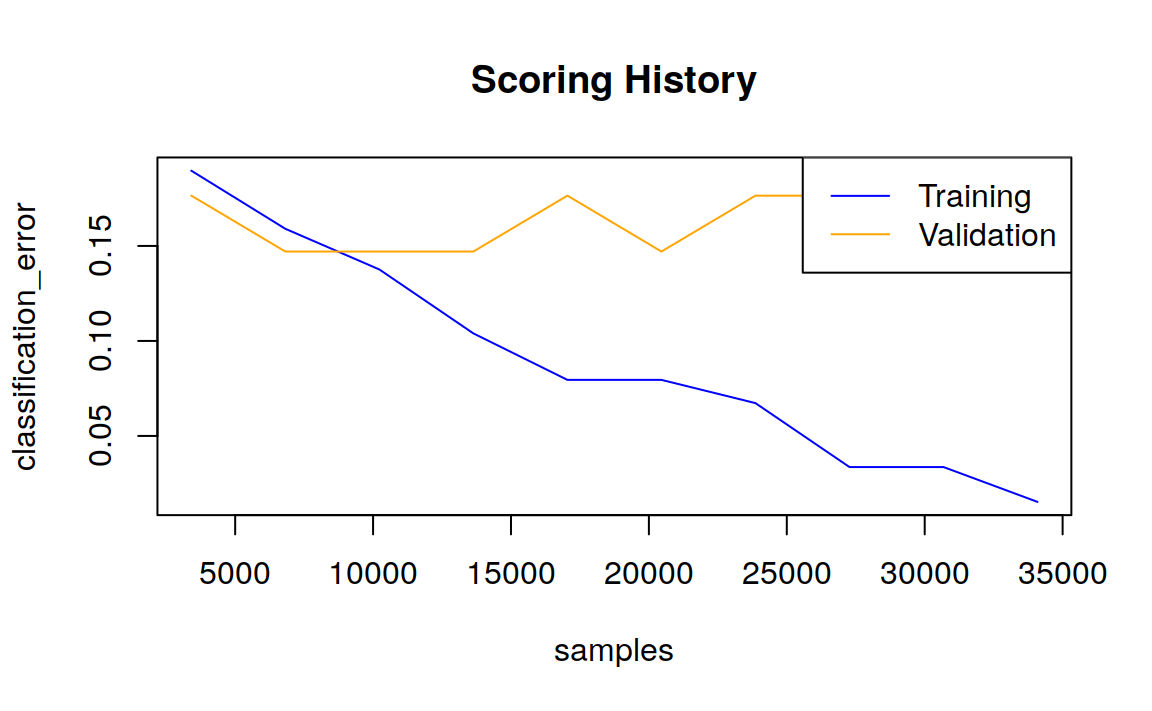
\includegraphics[width=0.7\linewidth]{meta_110b-PCA-Principal_Component_Methods_in_R_files/figure-latex/unnamed-chunk-21-1} 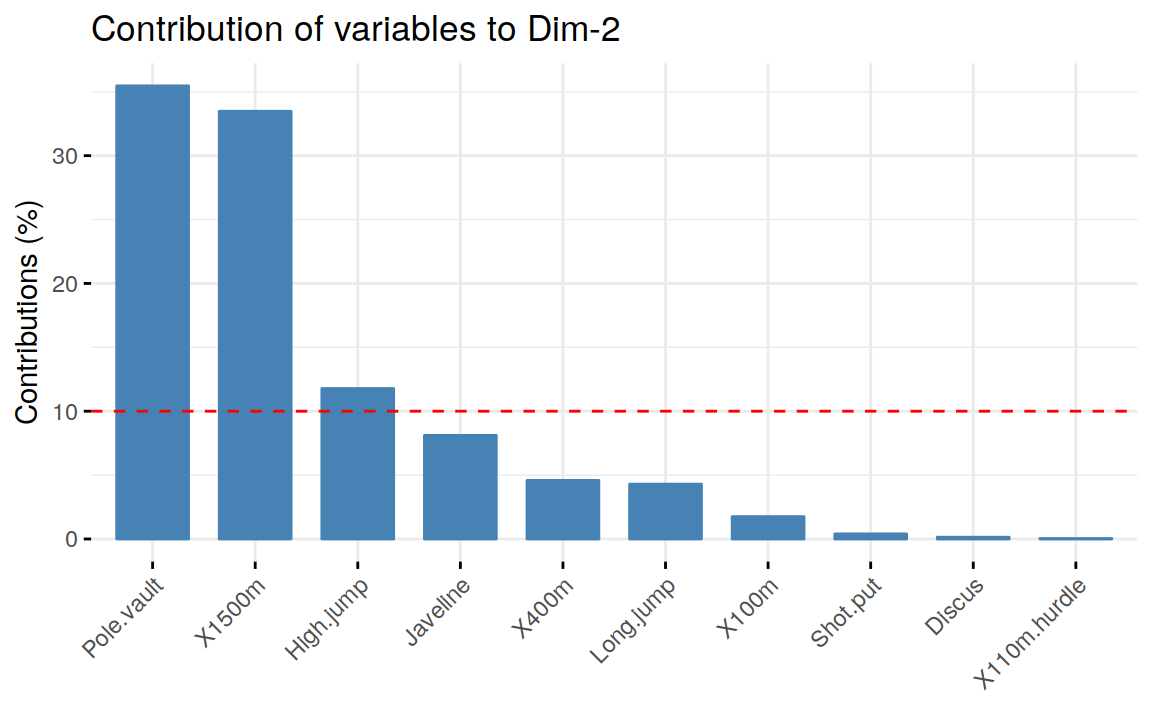
\includegraphics[width=0.7\linewidth]{meta_110b-PCA-Principal_Component_Methods_in_R_files/figure-latex/unnamed-chunk-21-2} \end{center}

The total contribution to PC1 and PC2 is obtained with the following R code:

\begin{Shaded}
\begin{Highlighting}[]
\KeywordTok{fviz_contrib}\NormalTok{(res.pca, }\DataTypeTok{choice =} \StringTok{"var"}\NormalTok{, }\DataTypeTok{axes =} \DecValTok{1}\OperatorTok{:}\DecValTok{2}\NormalTok{, }\DataTypeTok{top =} \DecValTok{10}\NormalTok{)}
\end{Highlighting}
\end{Shaded}

\begin{center}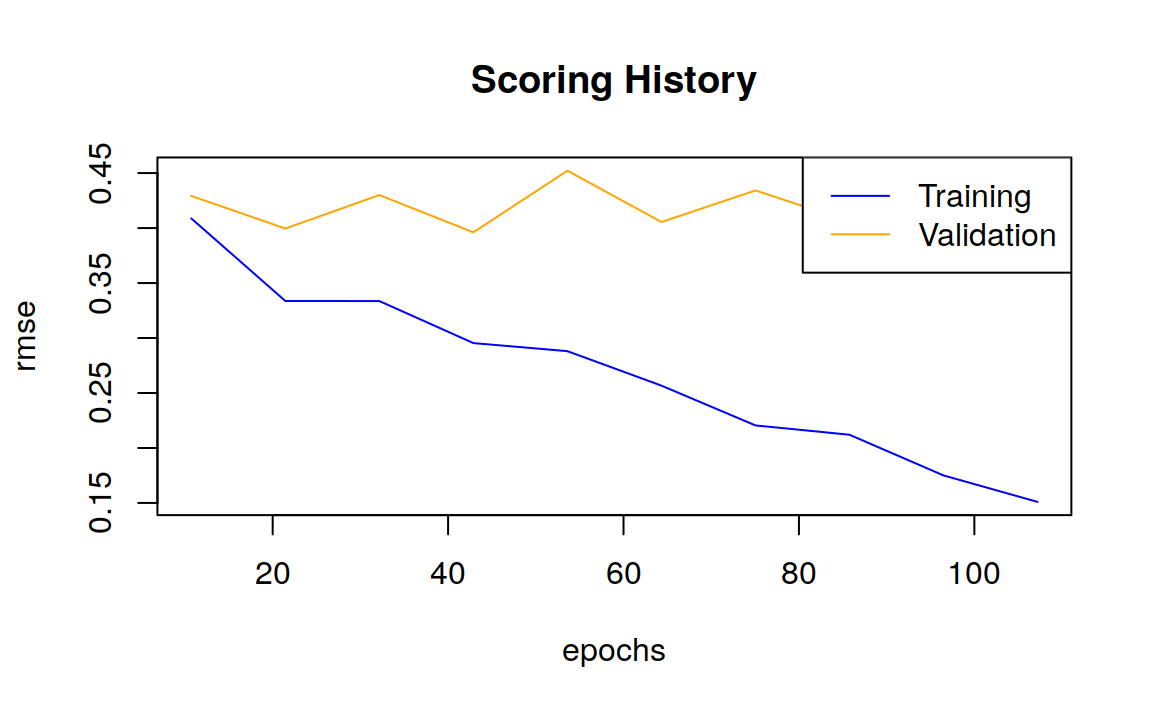
\includegraphics[width=0.7\linewidth]{meta_110b-PCA-Principal_Component_Methods_in_R_files/figure-latex/unnamed-chunk-22-1} \end{center}

The red dashed line on the graph above indicates the expected average contribution. If the contribution of the variables were uniform, the expected value would be 1/length(variables) = 1/10 = 10\%. For a given component, a variable with a contribution larger than this cutoff could be considered as important in contributing to the component.

Note that, the total contribution of a given variable, on explaining the variations retained by two principal components, say PC1 and PC2, is calculated as contrib = {[}(C1 * Eig1) + (C2 * Eig2){]}/(Eig1 + Eig2), where

\begin{itemize}
\tightlist
\item
  C1 and C2 are the contributions of the variable on PC1 and PC2, respectively
\item
  Eig1 and Eig2 are the eigenvalues of PC1 and PC2, respectively. Recall that eigenvalues measure the amount of variation retained by each PC.
\end{itemize}

In this case, the expected average contribution (cutoff) is calculated as follow: As mentioned above, if the contributions of the 10 variables were uniform, the expected average contribution on a given PC would be 1/10 = 10\%. The expected average contribution of a variable for PC1 and PC2 is : {[}(10* Eig1) + (10 * Eig2){]}/(Eig1 + Eig2)

It can be seen that the variables - X100m, Long.jump and Pole.vault - contribute the most to the dimensions 1 and 2.

The most important (or, contributing) variables can be highlighted on the correlation plot as follow:

\begin{Shaded}
\begin{Highlighting}[]
\KeywordTok{fviz_pca_var}\NormalTok{(res.pca, }\DataTypeTok{col.var =} \StringTok{"contrib"}\NormalTok{,}
             \DataTypeTok{gradient.cols =} \KeywordTok{c}\NormalTok{(}\StringTok{"#00AFBB"}\NormalTok{, }\StringTok{"#E7B800"}\NormalTok{, }\StringTok{"#FC4E07"}\NormalTok{)}
\NormalTok{             )}
\end{Highlighting}
\end{Shaded}

\begin{center}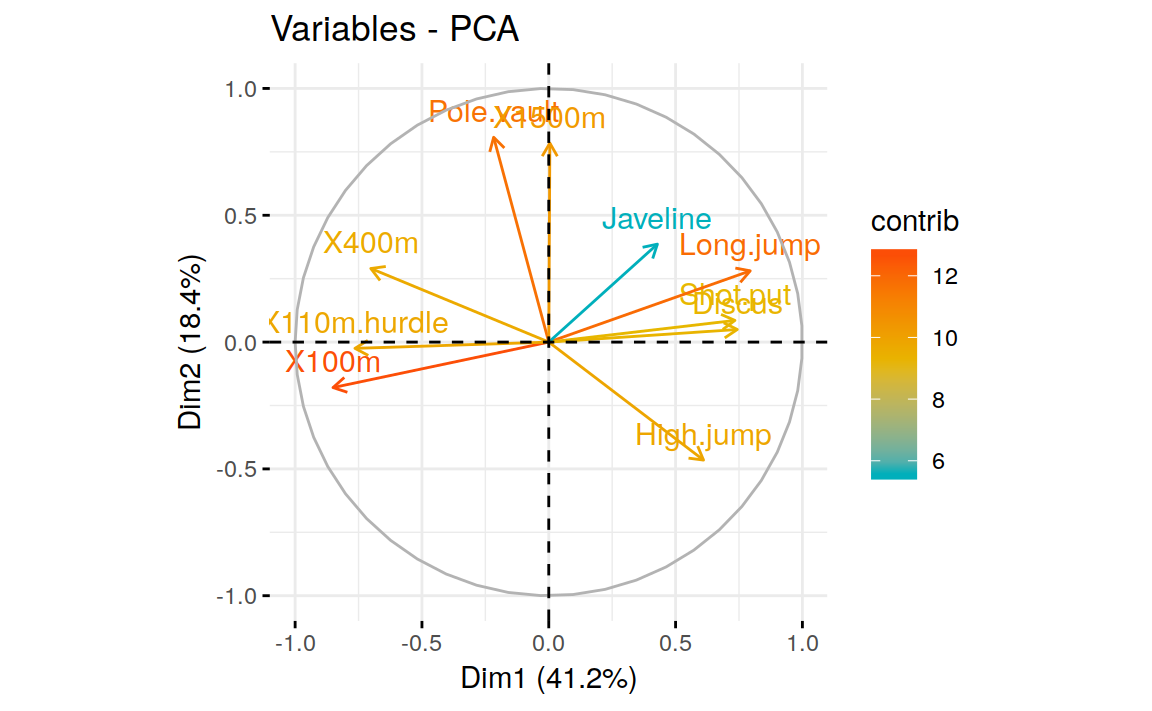
\includegraphics[width=0.7\linewidth]{meta_110b-PCA-Principal_Component_Methods_in_R_files/figure-latex/unnamed-chunk-23-1} \end{center}

Note that, it's also possible to change the transparency of variables according to their contrib values using the option alpha.var = ``contrib''. For example, type this:

\begin{Shaded}
\begin{Highlighting}[]
\CommentTok{# Change the transparency by contrib values}
\KeywordTok{fviz_pca_var}\NormalTok{(res.pca, }\DataTypeTok{alpha.var =} \StringTok{"contrib"}\NormalTok{)}
\end{Highlighting}
\end{Shaded}

\begin{center}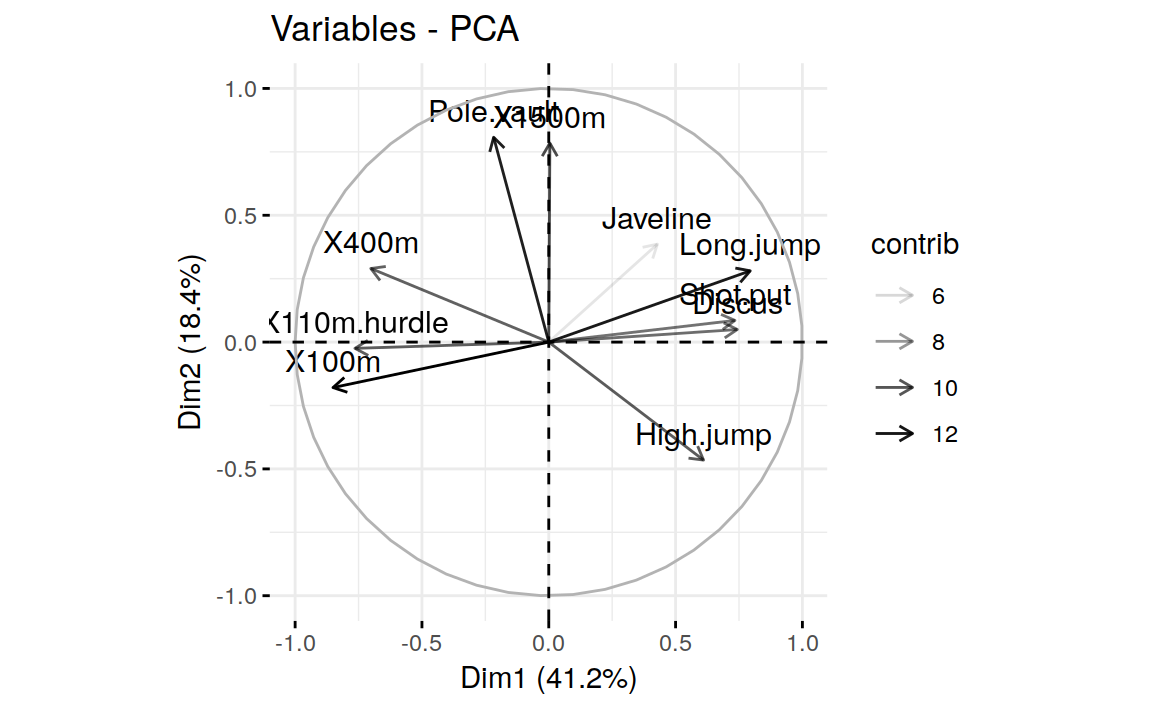
\includegraphics[width=0.7\linewidth]{meta_110b-PCA-Principal_Component_Methods_in_R_files/figure-latex/unnamed-chunk-24-1} \end{center}

\hypertarget{color-by-a-custom-continuous-variable}{%
\section{Color by a custom continuous variable}\label{color-by-a-custom-continuous-variable}}

In the previous sections, we showed how to color variables by their contributions and their cos2. Note that, it's possible to color variables by any custom continuous variable. The coloring variable should have the same length as the number of active variables in the PCA (here n = 10).

For example, type this:

\begin{Shaded}
\begin{Highlighting}[]
\CommentTok{# Create a random continuous variable of length 10}
\KeywordTok{set.seed}\NormalTok{(}\DecValTok{123}\NormalTok{)}
\NormalTok{my.cont.var <-}\StringTok{ }\KeywordTok{rnorm}\NormalTok{(}\DecValTok{10}\NormalTok{)}
\CommentTok{# Color variables by the continuous variable}
\KeywordTok{fviz_pca_var}\NormalTok{(res.pca, }\DataTypeTok{col.var =}\NormalTok{ my.cont.var,}
             \DataTypeTok{gradient.cols =} \KeywordTok{c}\NormalTok{(}\StringTok{"blue"}\NormalTok{, }\StringTok{"yellow"}\NormalTok{, }\StringTok{"red"}\NormalTok{),}
             \DataTypeTok{legend.title =} \StringTok{"Cont.Var"}\NormalTok{)}
\end{Highlighting}
\end{Shaded}

\begin{center}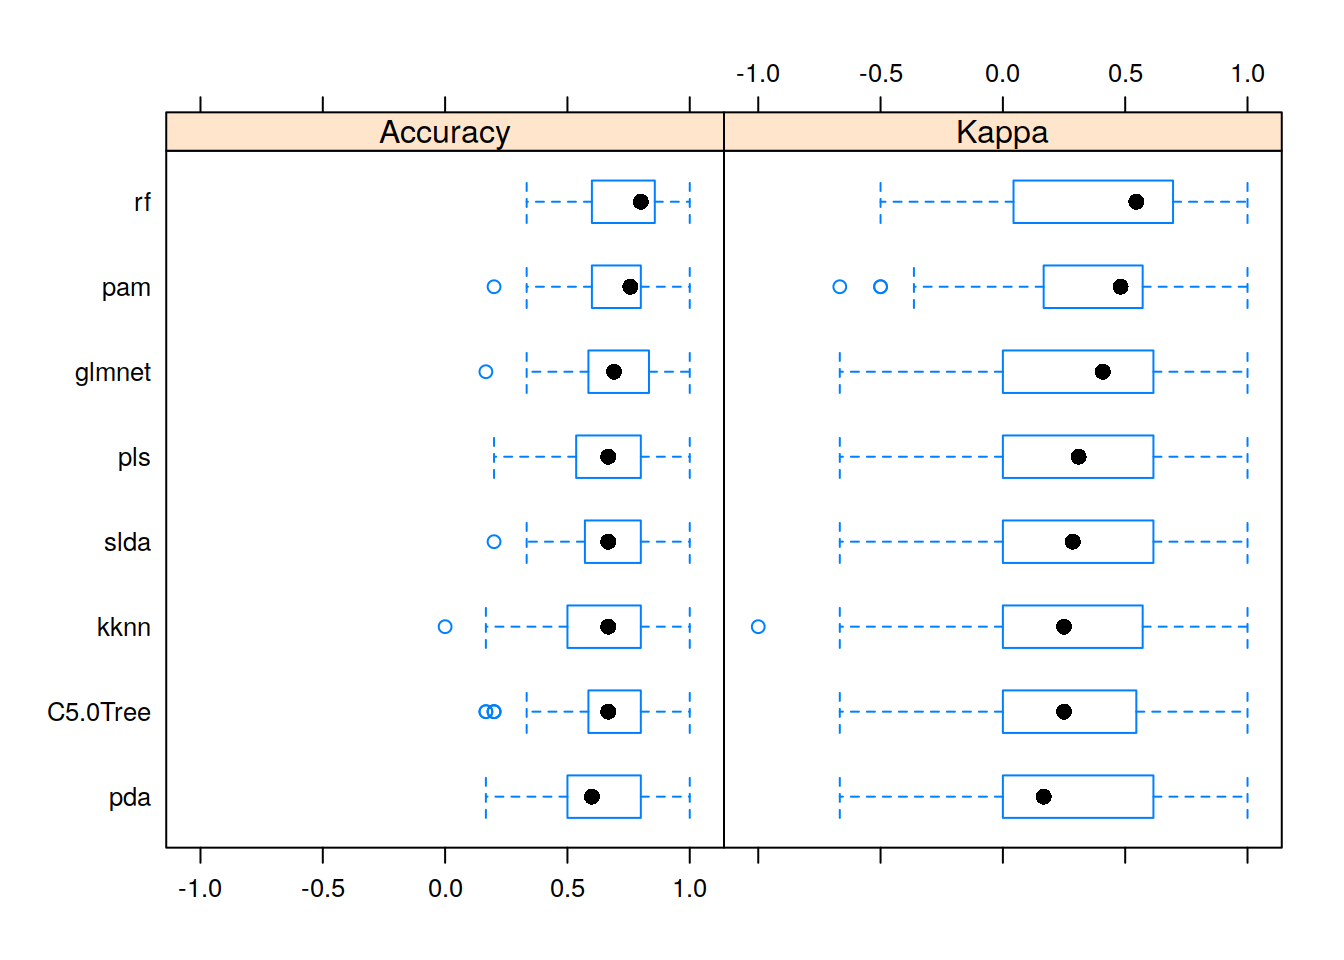
\includegraphics[width=0.7\linewidth]{meta_110b-PCA-Principal_Component_Methods_in_R_files/figure-latex/unnamed-chunk-25-1} \end{center}

\hypertarget{color-by-groups}{%
\section{Color by groups}\label{color-by-groups}}

It's also possible to change the color of variables by groups defined by a qualitative/categorical variable, also called factor in R terminology.

As we don't have any grouping variable in our data sets for classifying variables, we'll create it.

In the following demo example, we start by classifying the variables into 3 groups using the kmeans clustering algorithm. Next, we use the clusters returned by the kmeans algorithm to color variables.

\begin{Shaded}
\begin{Highlighting}[]
\CommentTok{# Create a grouping variable using kmeans}
\CommentTok{# Create 3 groups of variables (centers = 3)}
\KeywordTok{set.seed}\NormalTok{(}\DecValTok{123}\NormalTok{)}
\NormalTok{res.km <-}\StringTok{ }\KeywordTok{kmeans}\NormalTok{(var}\OperatorTok{$}\NormalTok{coord, }\DataTypeTok{centers =} \DecValTok{3}\NormalTok{, }\DataTypeTok{nstart =} \DecValTok{25}\NormalTok{)}
\NormalTok{grp <-}\StringTok{ }\KeywordTok{as.factor}\NormalTok{(res.km}\OperatorTok{$}\NormalTok{cluster)}
\CommentTok{# Color variables by groups}
\KeywordTok{fviz_pca_var}\NormalTok{(res.pca, }\DataTypeTok{col.var =}\NormalTok{ grp, }
             \DataTypeTok{palette =} \KeywordTok{c}\NormalTok{(}\StringTok{"#0073C2FF"}\NormalTok{, }\StringTok{"#EFC000FF"}\NormalTok{, }\StringTok{"#868686FF"}\NormalTok{),}
             \DataTypeTok{legend.title =} \StringTok{"Cluster"}\NormalTok{)}
\end{Highlighting}
\end{Shaded}

\begin{center}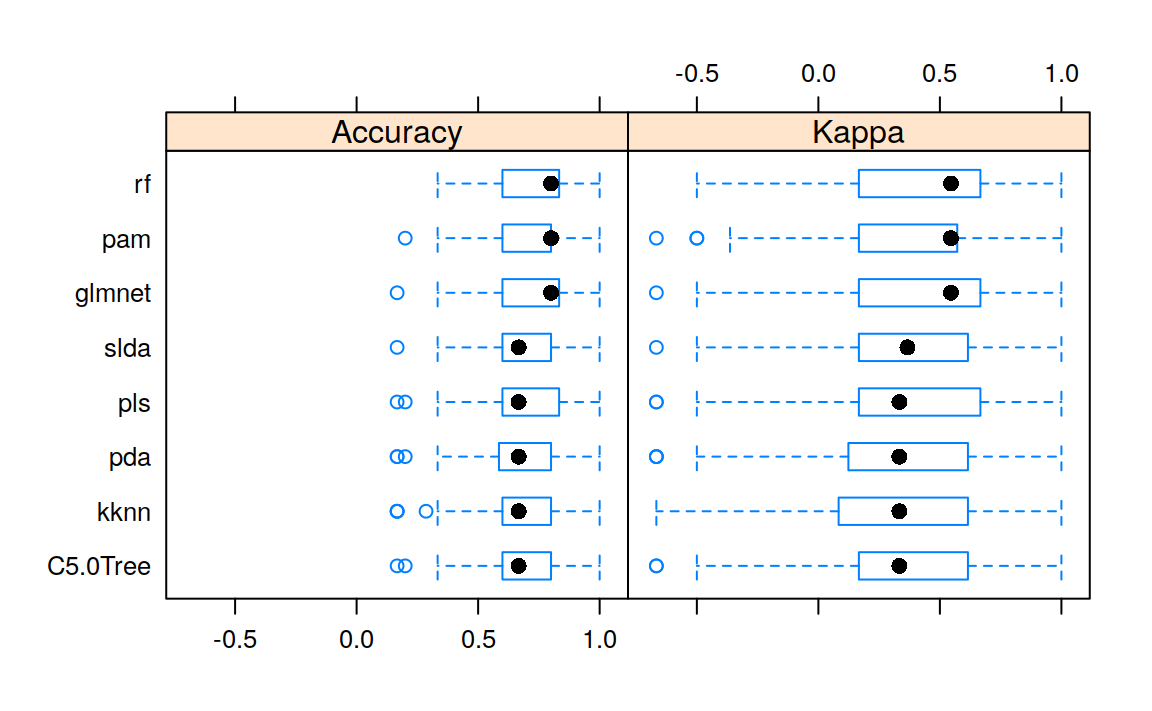
\includegraphics[width=0.7\linewidth]{meta_110b-PCA-Principal_Component_Methods_in_R_files/figure-latex/unnamed-chunk-26-1} \end{center}

\hypertarget{dimension-description}{%
\section{Dimension description}\label{dimension-description}}

In the section \citet{ref}(pca-variable-contributions), we described how to highlight variables according to their contributions to the principal components.

Note also that, the function dimdesc() {[}in FactoMineR{]}, for dimension description, can be used to identify the most significantly associated variables with a given principal component . It can be used as follow:

\begin{Shaded}
\begin{Highlighting}[]
\NormalTok{res.desc <-}\StringTok{ }\KeywordTok{dimdesc}\NormalTok{(res.pca, }\DataTypeTok{axes =} \KeywordTok{c}\NormalTok{(}\DecValTok{1}\NormalTok{,}\DecValTok{2}\NormalTok{), }\DataTypeTok{proba =} \FloatTok{0.05}\NormalTok{)}
\CommentTok{# Description of dimension 1}
\NormalTok{res.desc}\OperatorTok{$}\NormalTok{Dim}\FloatTok{.1}
\CommentTok{#> $quanti}
\CommentTok{#>              correlation  p.value}
\CommentTok{#> Long.jump          0.794 6.06e-06}
\CommentTok{#> Discus             0.743 4.84e-05}
\CommentTok{#> Shot.put           0.734 6.72e-05}
\CommentTok{#> High.jump          0.610 1.99e-03}
\CommentTok{#> Javeline           0.428 4.15e-02}
\CommentTok{#> X400m             -0.702 1.91e-04}
\CommentTok{#> X110m.hurdle      -0.764 2.20e-05}
\CommentTok{#> X100m             -0.851 2.73e-07}
\end{Highlighting}
\end{Shaded}

\begin{Shaded}
\begin{Highlighting}[]
\CommentTok{# Description of dimension 2}
\NormalTok{res.desc}\OperatorTok{$}\NormalTok{Dim}\FloatTok{.2}
\CommentTok{#> $quanti}
\CommentTok{#>            correlation  p.value}
\CommentTok{#> Pole.vault       0.807 3.21e-06}
\CommentTok{#> X1500m           0.784 9.38e-06}
\CommentTok{#> High.jump       -0.465 2.53e-02}
\end{Highlighting}
\end{Shaded}

\hypertarget{graph-of-individuals}{%
\section{Graph of individuals}\label{graph-of-individuals}}

Results
The results, for individuals can be extracted using the function get\_pca\_ind() {[}factoextra package{]}. Similarly to the get\_pca\_var(), the function get\_pca\_ind() provides a list of matrices containing all the results for the individuals (coordinates, correlation between individuals and axes, squared cosine and contributions)

\begin{Shaded}
\begin{Highlighting}[]
\NormalTok{ind <-}\StringTok{ }\KeywordTok{get_pca_ind}\NormalTok{(res.pca)}
\NormalTok{ind}
\CommentTok{#> Principal Component Analysis Results for individuals}
\CommentTok{#>  ===================================================}
\CommentTok{#>   Name       Description                       }
\CommentTok{#> 1 "$coord"   "Coordinates for the individuals" }
\CommentTok{#> 2 "$cos2"    "Cos2 for the individuals"        }
\CommentTok{#> 3 "$contrib" "contributions of the individuals"}
\end{Highlighting}
\end{Shaded}

To get access to the different components, use this:

\begin{Shaded}
\begin{Highlighting}[]
\CommentTok{# Coordinates of individuals}
\KeywordTok{head}\NormalTok{(ind}\OperatorTok{$}\NormalTok{coord)}
\CommentTok{#>            Dim.1  Dim.2  Dim.3   Dim.4   Dim.5}
\CommentTok{#> SEBRLE     0.196  1.589  0.642  0.0839  1.1683}
\CommentTok{#> CLAY       0.808  2.475 -1.387  1.2984 -0.8250}
\CommentTok{#> BERNARD   -1.359  1.648  0.201 -1.9641  0.0842}
\CommentTok{#> YURKOV    -0.889 -0.443  2.530  0.7129  0.4078}
\CommentTok{#> ZSIVOCZKY -0.108 -2.069 -1.334 -0.1015 -0.2015}
\CommentTok{#> McMULLEN   0.121 -1.014 -0.863  1.3416  1.6215}
\CommentTok{# Quality of individuals}
\KeywordTok{head}\NormalTok{(ind}\OperatorTok{$}\NormalTok{cos2)}
\CommentTok{#>             Dim.1  Dim.2   Dim.3   Dim.4    Dim.5}
\CommentTok{#> SEBRLE    0.00753 0.4975 0.08133 0.00139 0.268903}
\CommentTok{#> CLAY      0.04870 0.4570 0.14363 0.12579 0.050785}
\CommentTok{#> BERNARD   0.19720 0.2900 0.00429 0.41182 0.000757}
\CommentTok{#> YURKOV    0.09611 0.0238 0.77823 0.06181 0.020228}
\CommentTok{#> ZSIVOCZKY 0.00157 0.5764 0.23975 0.00139 0.005465}
\CommentTok{#> McMULLEN  0.00218 0.1522 0.11014 0.26649 0.389262}
\CommentTok{# Contributions of individuals}
\KeywordTok{head}\NormalTok{(ind}\OperatorTok{$}\NormalTok{contrib)}
\CommentTok{#>            Dim.1  Dim.2  Dim.3   Dim.4   Dim.5}
\CommentTok{#> SEBRLE    0.0403  5.971  1.448  0.0373  8.4589}
\CommentTok{#> CLAY      0.6881 14.484  6.754  8.9446  4.2179}
\CommentTok{#> BERNARD   1.9474  6.423  0.141 20.4682  0.0439}
\CommentTok{#> YURKOV    0.8331  0.463 22.452  2.6966  1.0308}
\CommentTok{#> ZSIVOCZKY 0.0123 10.122  6.246  0.0547  0.2515}
\CommentTok{#> McMULLEN  0.0155  2.431  2.610  9.5506 16.2949}
\end{Highlighting}
\end{Shaded}

\hypertarget{plots-quality-and-contribution-1}{%
\section{Plots: quality and contribution}\label{plots-quality-and-contribution-1}}

The fviz\_pca\_ind() is used to produce the graph of individuals. To create a simple plot, type this:

\begin{Shaded}
\begin{Highlighting}[]
\KeywordTok{fviz_pca_ind}\NormalTok{(res.pca)}
\end{Highlighting}
\end{Shaded}

\begin{center}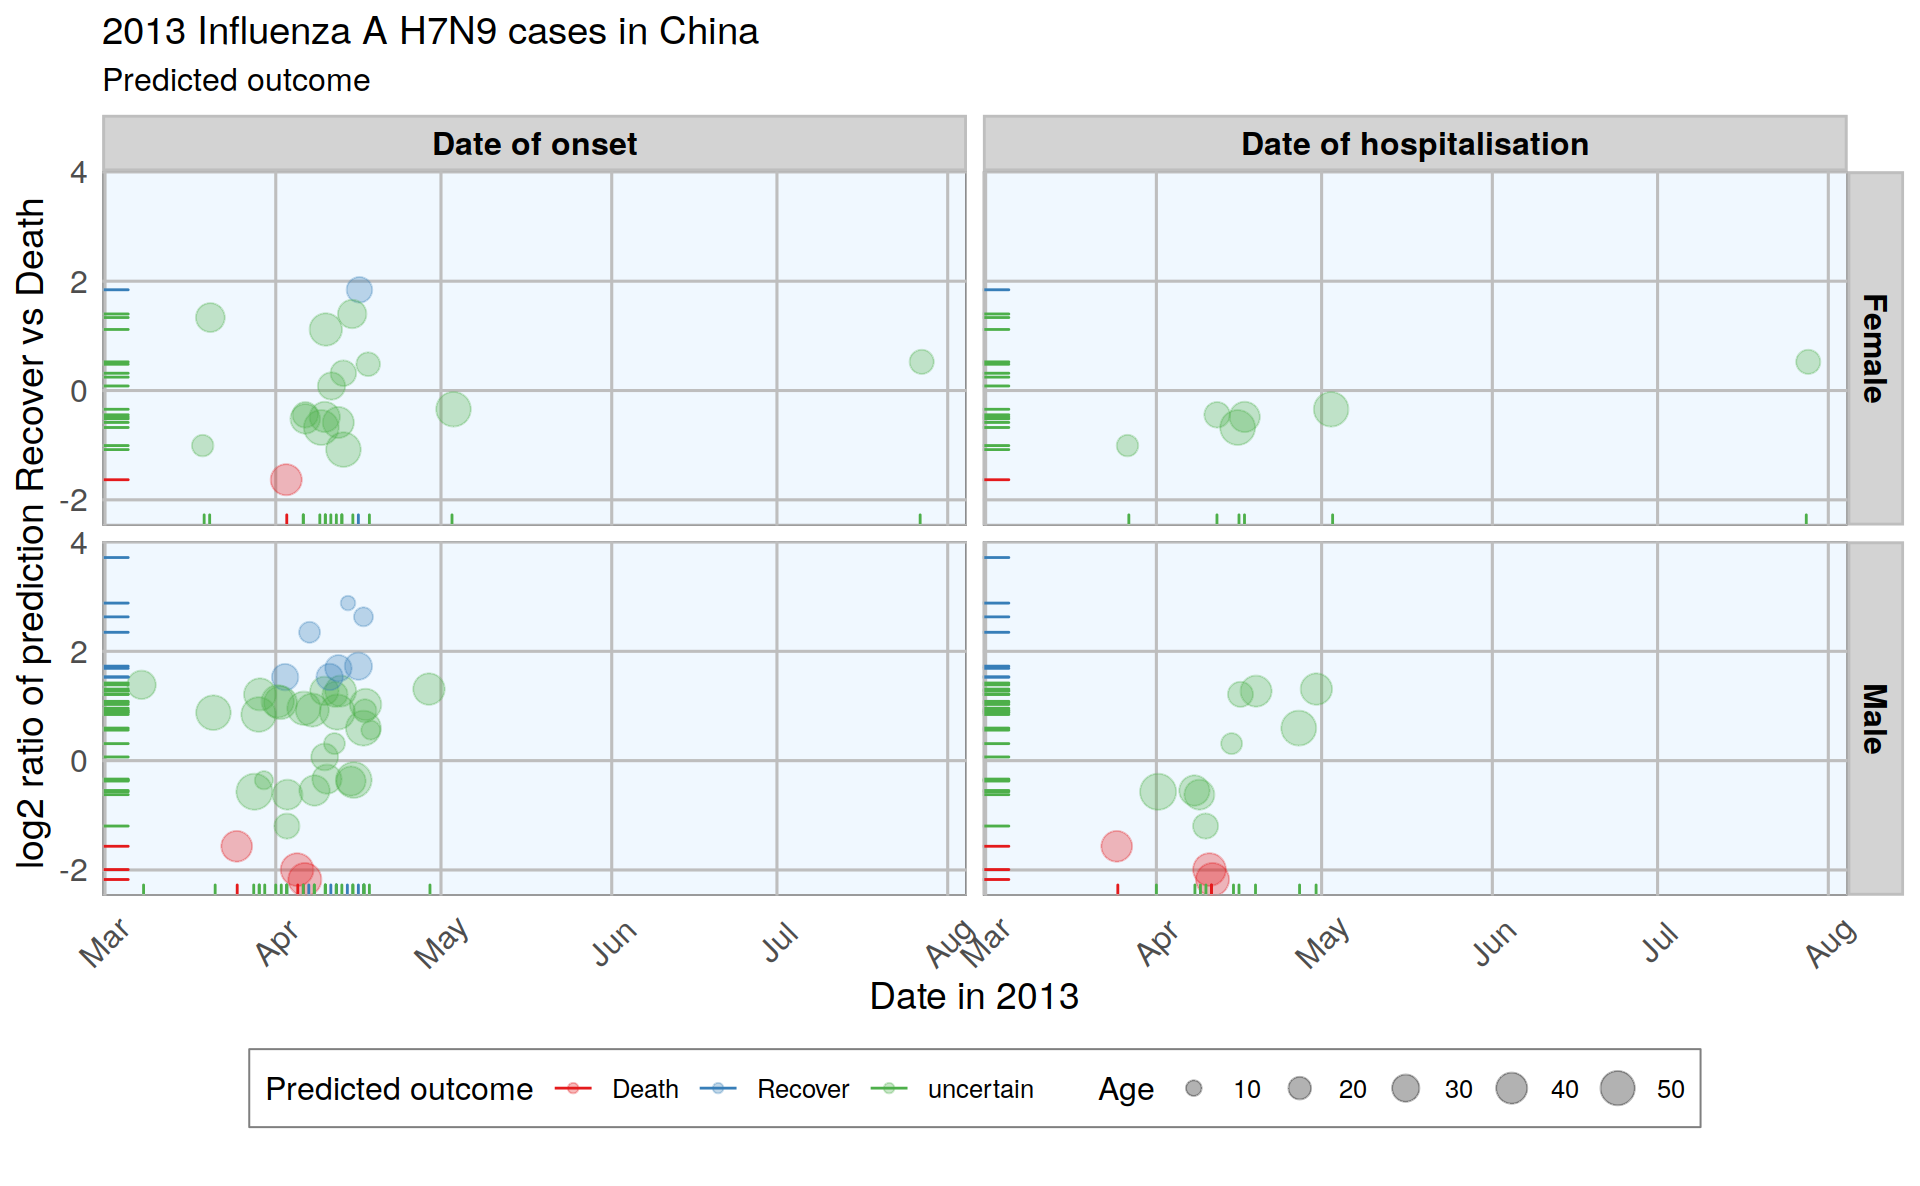
\includegraphics[width=0.7\linewidth]{meta_110b-PCA-Principal_Component_Methods_in_R_files/figure-latex/unnamed-chunk-31-1} \end{center}

Like variables, it's also possible to color individuals by their cos2 values:

\begin{Shaded}
\begin{Highlighting}[]
\KeywordTok{fviz_pca_ind}\NormalTok{(res.pca, }\DataTypeTok{col.ind =} \StringTok{"cos2"}\NormalTok{, }
             \DataTypeTok{gradient.cols =} \KeywordTok{c}\NormalTok{(}\StringTok{"#00AFBB"}\NormalTok{, }\StringTok{"#E7B800"}\NormalTok{, }\StringTok{"#FC4E07"}\NormalTok{),}
             \DataTypeTok{repel =} \OtherTok{TRUE} \CommentTok{# Avoid text overlapping (slow if many points)}
\NormalTok{             )}
\end{Highlighting}
\end{Shaded}

\begin{center}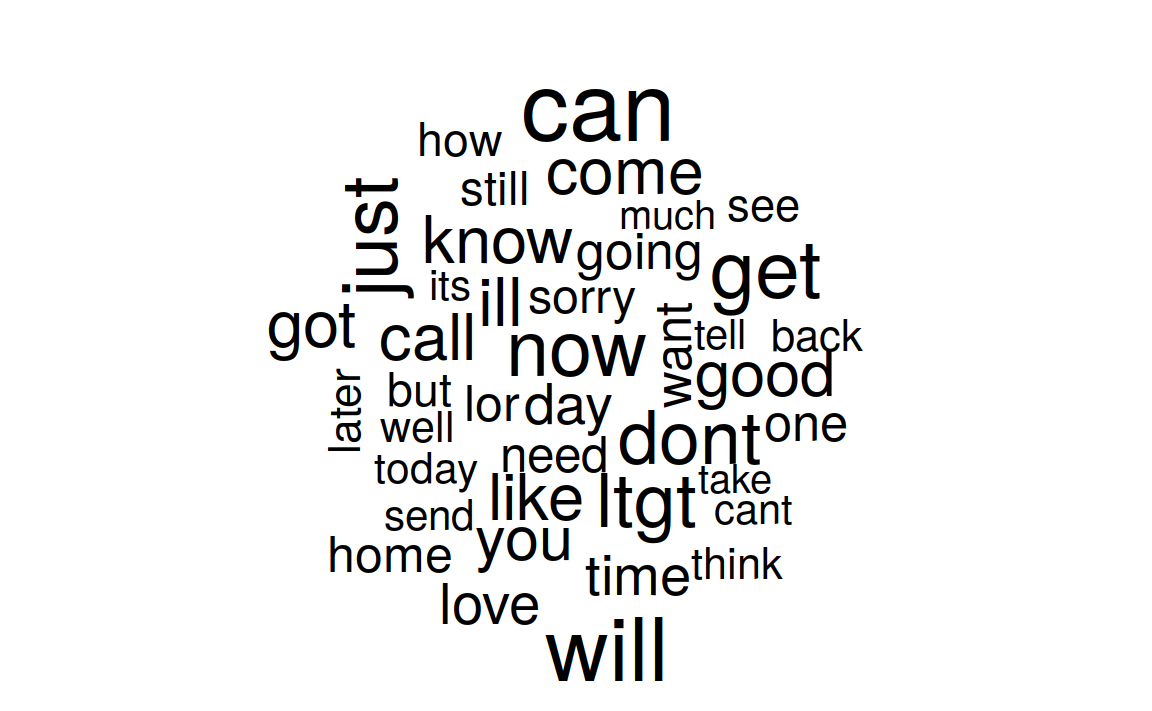
\includegraphics[width=0.7\linewidth]{meta_110b-PCA-Principal_Component_Methods_in_R_files/figure-latex/unnamed-chunk-32-1} \end{center}

\begin{quote}
Note that, individuals that are similar are grouped together on the plot.
\end{quote}

You can also change the point size according the cos2 of the corresponding individuals:

\begin{Shaded}
\begin{Highlighting}[]
\KeywordTok{fviz_pca_ind}\NormalTok{(res.pca, }\DataTypeTok{pointsize =} \StringTok{"cos2"}\NormalTok{, }
             \DataTypeTok{pointshape =} \DecValTok{21}\NormalTok{, }\DataTypeTok{fill =} \StringTok{"#E7B800"}\NormalTok{,}
             \DataTypeTok{repel =} \OtherTok{TRUE} \CommentTok{# Avoid text overlapping (slow if many points)}
\NormalTok{             )}
\end{Highlighting}
\end{Shaded}

\begin{center}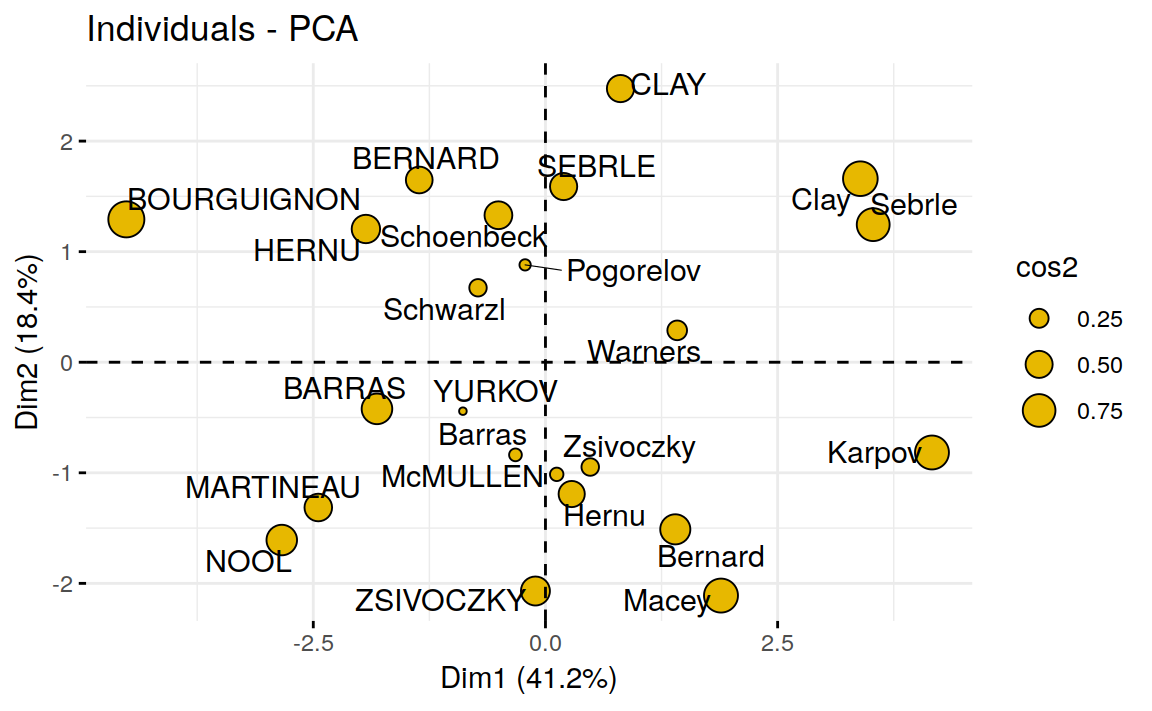
\includegraphics[width=0.7\linewidth]{meta_110b-PCA-Principal_Component_Methods_in_R_files/figure-latex/unnamed-chunk-33-1} \end{center}

To change both point size and color by cos2, try this:

\begin{Shaded}
\begin{Highlighting}[]
\KeywordTok{fviz_pca_ind}\NormalTok{(res.pca, }\DataTypeTok{col.ind =} \StringTok{"cos2"}\NormalTok{, }\DataTypeTok{pointsize =} \StringTok{"cos2"}\NormalTok{,}
             \DataTypeTok{gradient.cols =} \KeywordTok{c}\NormalTok{(}\StringTok{"#00AFBB"}\NormalTok{, }\StringTok{"#E7B800"}\NormalTok{, }\StringTok{"#FC4E07"}\NormalTok{),}
             \DataTypeTok{repel =} \OtherTok{TRUE} \CommentTok{# Avoid text overlapping (slow if many points)}
\NormalTok{             )}
\end{Highlighting}
\end{Shaded}

\begin{center}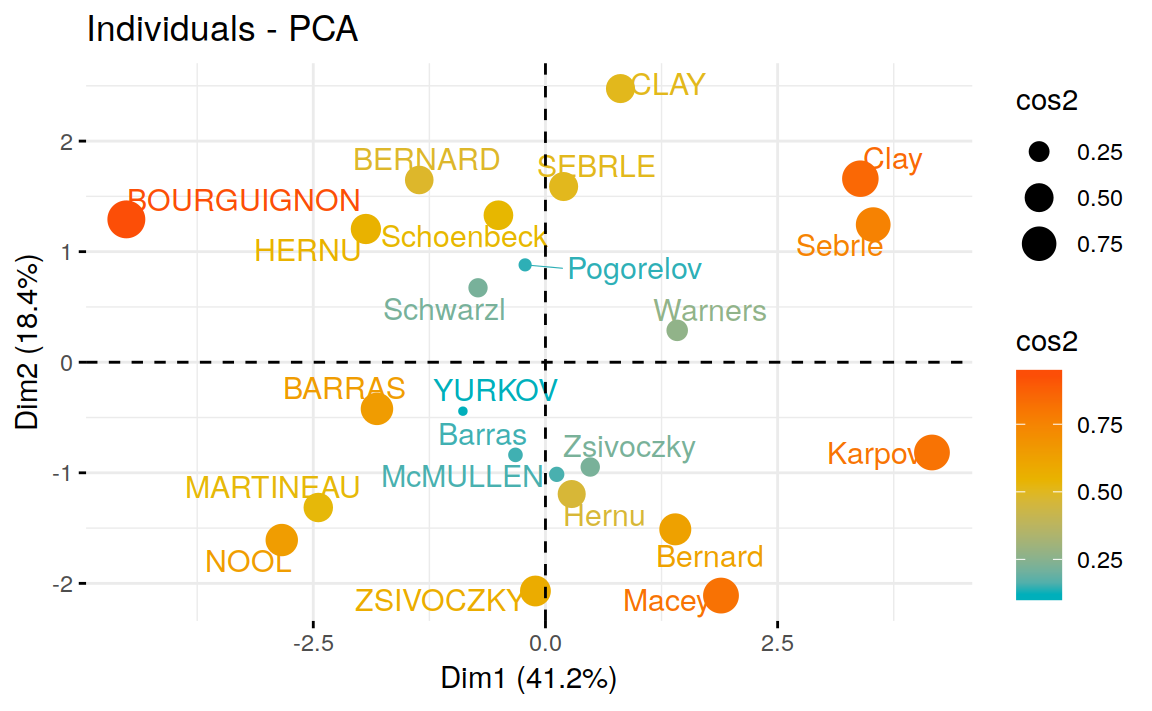
\includegraphics[width=0.7\linewidth]{meta_110b-PCA-Principal_Component_Methods_in_R_files/figure-latex/unnamed-chunk-34-1} \end{center}

To create a bar plot of the quality of representation (cos2) of individuals on the factor map, you can use the function fviz\_cos2() as previously described for variables:

\begin{Shaded}
\begin{Highlighting}[]
\KeywordTok{fviz_cos2}\NormalTok{(res.pca, }\DataTypeTok{choice =} \StringTok{"ind"}\NormalTok{)}
\end{Highlighting}
\end{Shaded}

\begin{center}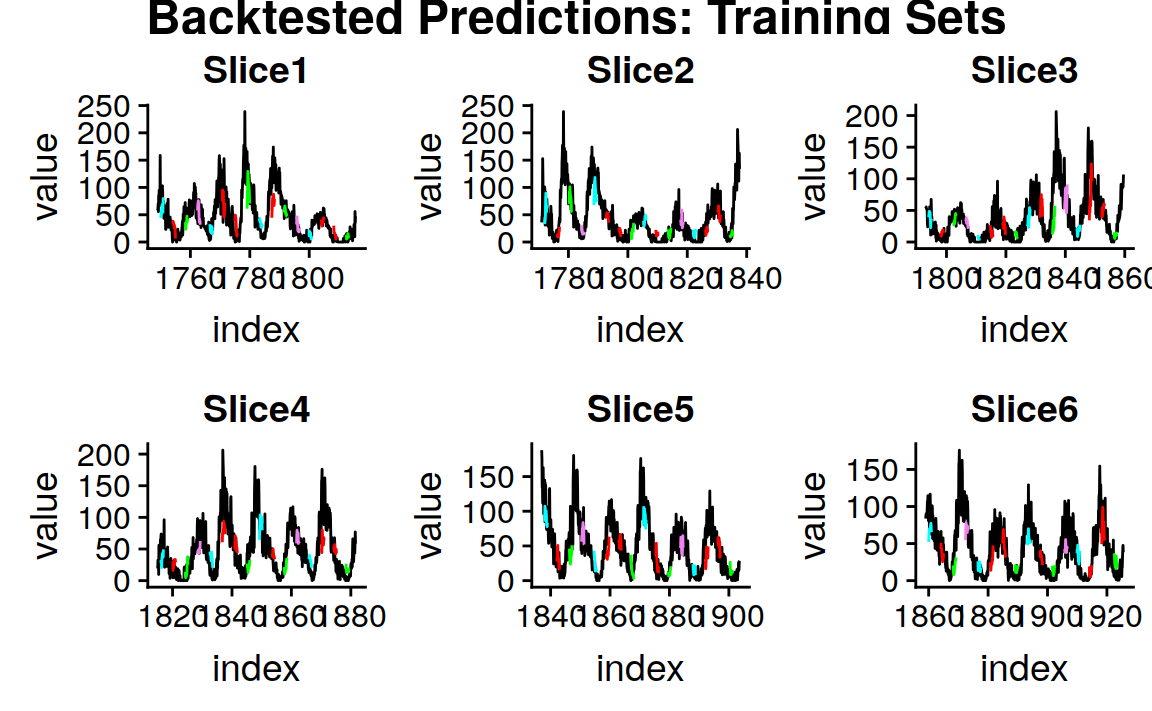
\includegraphics[width=0.7\linewidth]{meta_110b-PCA-Principal_Component_Methods_in_R_files/figure-latex/unnamed-chunk-35-1} \end{center}

To visualize the contribution of individuals to the first two principal components, type this:

\begin{Shaded}
\begin{Highlighting}[]
\CommentTok{# Total contribution on PC1 and PC2}
\KeywordTok{fviz_contrib}\NormalTok{(res.pca, }\DataTypeTok{choice =} \StringTok{"ind"}\NormalTok{, }\DataTypeTok{axes =} \DecValTok{1}\OperatorTok{:}\DecValTok{2}\NormalTok{)}
\end{Highlighting}
\end{Shaded}

\begin{center}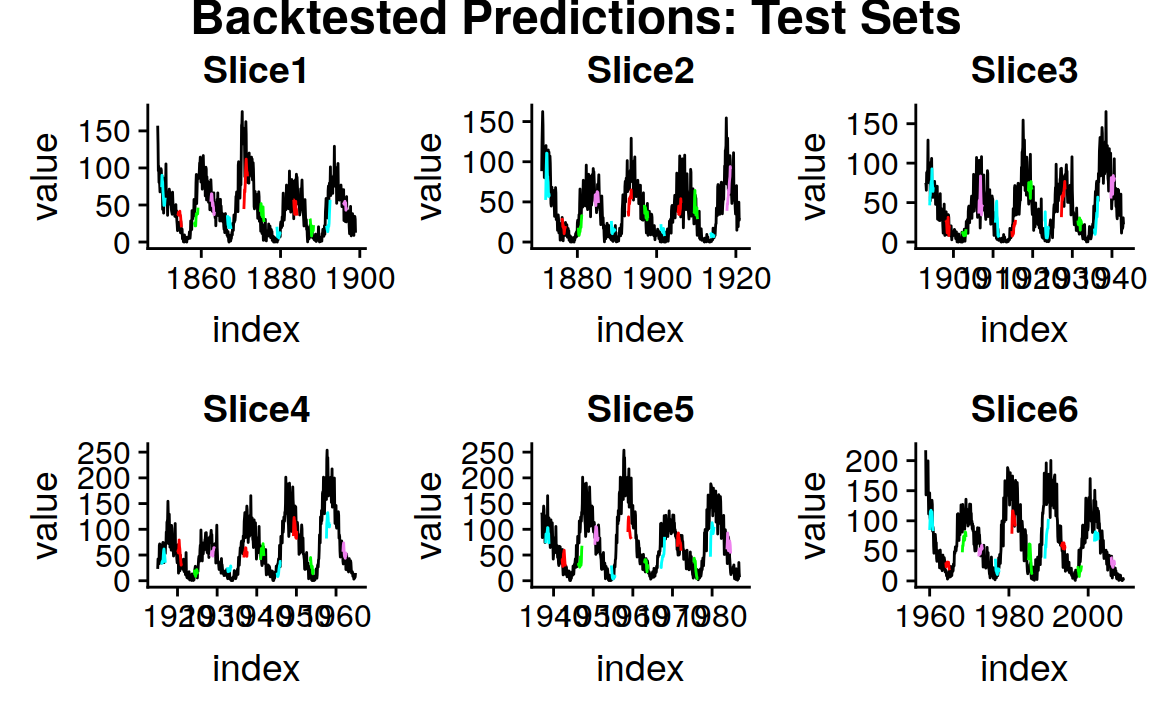
\includegraphics[width=0.7\linewidth]{meta_110b-PCA-Principal_Component_Methods_in_R_files/figure-latex/unnamed-chunk-36-1} \end{center}

\hypertarget{color-by-a-custom-continuous-variable-1}{%
\section{Color by a custom continuous variable}\label{color-by-a-custom-continuous-variable-1}}

As for variables, individuals can be colored by any custom continuous variable by specifying the argument col.ind.

For example, type this:

\begin{Shaded}
\begin{Highlighting}[]
\CommentTok{# Create a random continuous variable of length 23,}
\CommentTok{# Same length as the number of active individuals in the PCA}
\KeywordTok{set.seed}\NormalTok{(}\DecValTok{123}\NormalTok{)}
\NormalTok{my.cont.var <-}\StringTok{ }\KeywordTok{rnorm}\NormalTok{(}\DecValTok{23}\NormalTok{)}
\CommentTok{# Color individuals by the continuous variable}
\KeywordTok{fviz_pca_ind}\NormalTok{(res.pca, }\DataTypeTok{col.ind =}\NormalTok{ my.cont.var,}
             \DataTypeTok{gradient.cols =} \KeywordTok{c}\NormalTok{(}\StringTok{"blue"}\NormalTok{, }\StringTok{"yellow"}\NormalTok{, }\StringTok{"red"}\NormalTok{),}
             \DataTypeTok{legend.title =} \StringTok{"Cont.Var"}\NormalTok{)}
\end{Highlighting}
\end{Shaded}

\begin{center}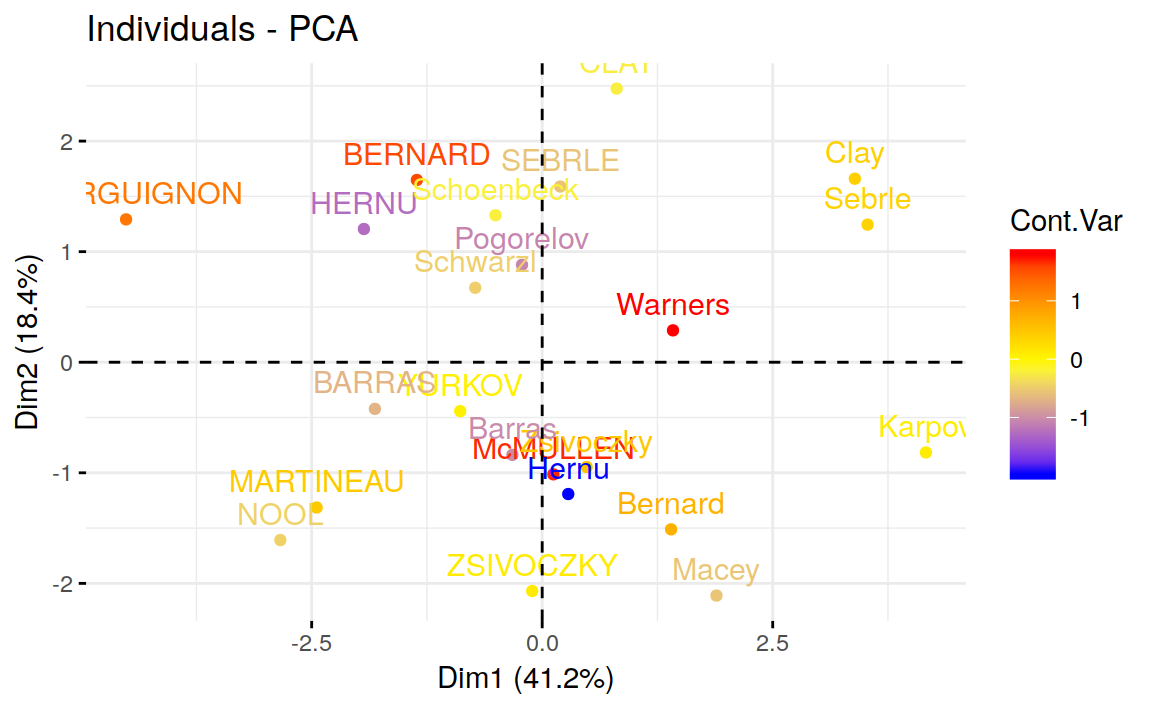
\includegraphics[width=0.7\linewidth]{meta_110b-PCA-Principal_Component_Methods_in_R_files/figure-latex/unnamed-chunk-37-1} \end{center}

\hypertarget{color-by-groups-1}{%
\section{Color by groups}\label{color-by-groups-1}}

Here, we describe how to color individuals by group. Additionally, we show how to add concentration ellipses and confidence ellipses by groups. For this, we'll use the iris data as demo data sets.

Iris data sets look like this:

\begin{Shaded}
\begin{Highlighting}[]
\KeywordTok{head}\NormalTok{(iris, }\DecValTok{3}\NormalTok{)}
\CommentTok{#>   Sepal.Length Sepal.Width Petal.Length Petal.Width Species}
\CommentTok{#> 1          5.1         3.5          1.4         0.2  setosa}
\CommentTok{#> 2          4.9         3.0          1.4         0.2  setosa}
\CommentTok{#> 3          4.7         3.2          1.3         0.2  setosa}
\end{Highlighting}
\end{Shaded}

The column ``Species'' will be used as grouping variable. We start by computing principal component analysis as follow:

\begin{Shaded}
\begin{Highlighting}[]
\CommentTok{# The variable Species (index = 5) is removed}
\CommentTok{# before PCA analysis}
\NormalTok{iris.pca <-}\StringTok{ }\KeywordTok{PCA}\NormalTok{(iris[,}\OperatorTok{-}\DecValTok{5}\NormalTok{], }\DataTypeTok{graph =} \OtherTok{FALSE}\NormalTok{)}
\end{Highlighting}
\end{Shaded}

In the R code below: the argument habillage or col.ind can be used to specify the factor variable for coloring the individuals by groups.

To add a concentration ellipse around each group, specify the argument addEllipses = TRUE. The argument palette can be used to change group colors.

\begin{Shaded}
\begin{Highlighting}[]
\KeywordTok{fviz_pca_ind}\NormalTok{(iris.pca,}
             \DataTypeTok{geom.ind =} \StringTok{"point"}\NormalTok{, }\CommentTok{# show points only (nbut not "text")}
             \DataTypeTok{col.ind =}\NormalTok{ iris}\OperatorTok{$}\NormalTok{Species, }\CommentTok{# color by groups}
             \DataTypeTok{palette =} \KeywordTok{c}\NormalTok{(}\StringTok{"#00AFBB"}\NormalTok{, }\StringTok{"#E7B800"}\NormalTok{, }\StringTok{"#FC4E07"}\NormalTok{),}
             \DataTypeTok{addEllipses =} \OtherTok{TRUE}\NormalTok{, }\CommentTok{# Concentration ellipses}
             \DataTypeTok{legend.title =} \StringTok{"Groups"}
\NormalTok{             )}
\end{Highlighting}
\end{Shaded}

\begin{center}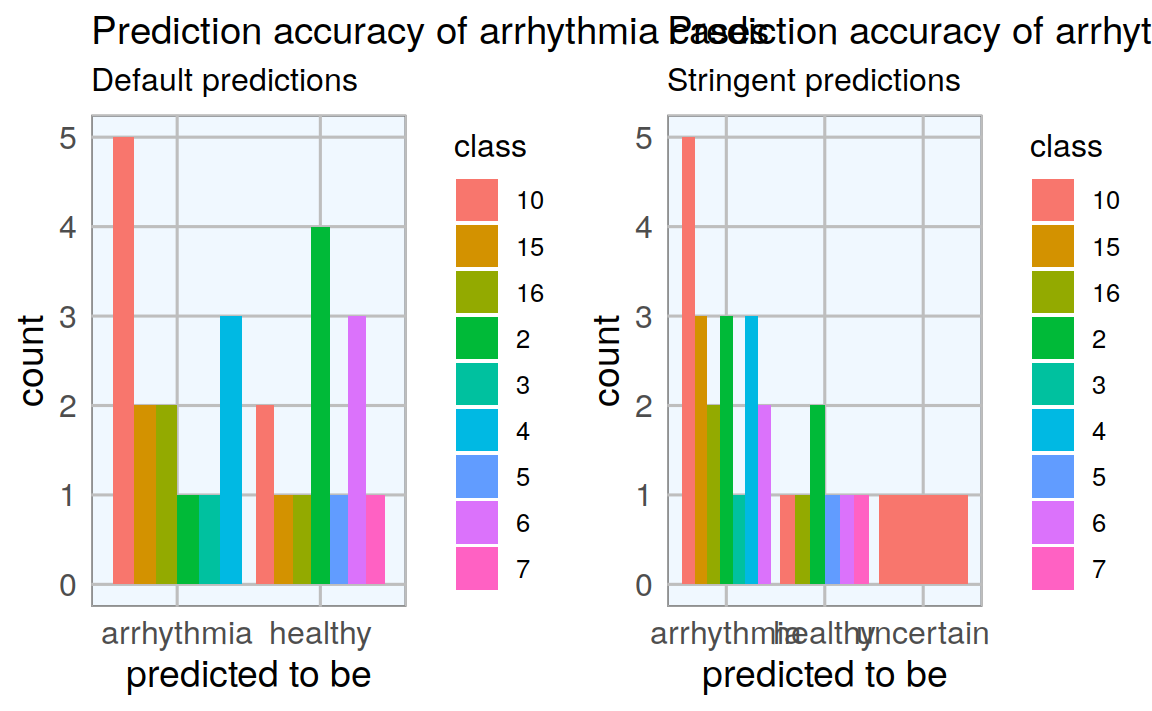
\includegraphics[width=0.7\linewidth]{meta_110b-PCA-Principal_Component_Methods_in_R_files/figure-latex/unnamed-chunk-40-1} \end{center}

\begin{quote}
To remove the group mean point, specify the argument mean.point = FALSE.
If you want confidence ellipses instead of concentration ellipses, use ellipse.type = ``confidence''.
\end{quote}

\begin{Shaded}
\begin{Highlighting}[]
\CommentTok{# Add confidence ellipses}
\KeywordTok{fviz_pca_ind}\NormalTok{(iris.pca, }\DataTypeTok{geom.ind =} \StringTok{"point"}\NormalTok{, }\DataTypeTok{col.ind =}\NormalTok{ iris}\OperatorTok{$}\NormalTok{Species, }
             \DataTypeTok{palette =} \KeywordTok{c}\NormalTok{(}\StringTok{"#00AFBB"}\NormalTok{, }\StringTok{"#E7B800"}\NormalTok{, }\StringTok{"#FC4E07"}\NormalTok{),}
             \DataTypeTok{addEllipses =} \OtherTok{TRUE}\NormalTok{, }\DataTypeTok{ellipse.type =} \StringTok{"confidence"}\NormalTok{,}
             \DataTypeTok{legend.title =} \StringTok{"Groups"}
\NormalTok{             )}
\end{Highlighting}
\end{Shaded}

\begin{center}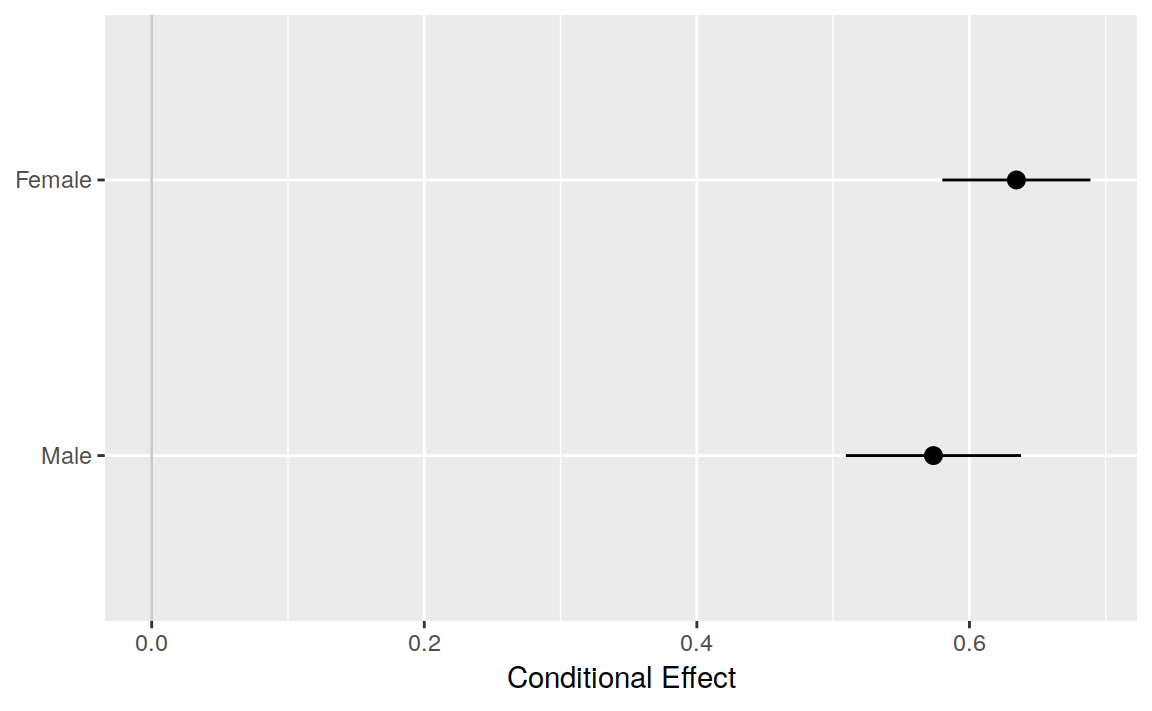
\includegraphics[width=0.7\linewidth]{meta_110b-PCA-Principal_Component_Methods_in_R_files/figure-latex/unnamed-chunk-41-1} \end{center}

Note that, allowed values for palette include:

\begin{itemize}
\tightlist
\item
  ``grey'' for grey color palettes;
\item
  brewer palettes e.g. ``RdBu'', ``Blues'', \ldots{}; To view all, type this in R: RColorBrewer::display.brewer.all().
\item
  custom color palette e.g.~c(``blue'', ``red'');
  and scientific journal palettes from ggsci R package, e.g.: ``npg'', ``aaas'', * ``lancet'', ``jco'', ``ucscgb'', ``uchicago'', ``simpsons'' and ``rickandmorty''.
  For example, to use the jco (journal of clinical oncology) color palette, type this:
\end{itemize}

\begin{Shaded}
\begin{Highlighting}[]
\KeywordTok{fviz_pca_ind}\NormalTok{(iris.pca,}
             \DataTypeTok{label =} \StringTok{"none"}\NormalTok{, }\CommentTok{# hide individual labels}
             \DataTypeTok{habillage =}\NormalTok{ iris}\OperatorTok{$}\NormalTok{Species, }\CommentTok{# color by groups}
             \DataTypeTok{addEllipses =} \OtherTok{TRUE}\NormalTok{, }\CommentTok{# Concentration ellipses}
             \DataTypeTok{palette =} \StringTok{"jco"}
\NormalTok{             )}
\end{Highlighting}
\end{Shaded}

\begin{center}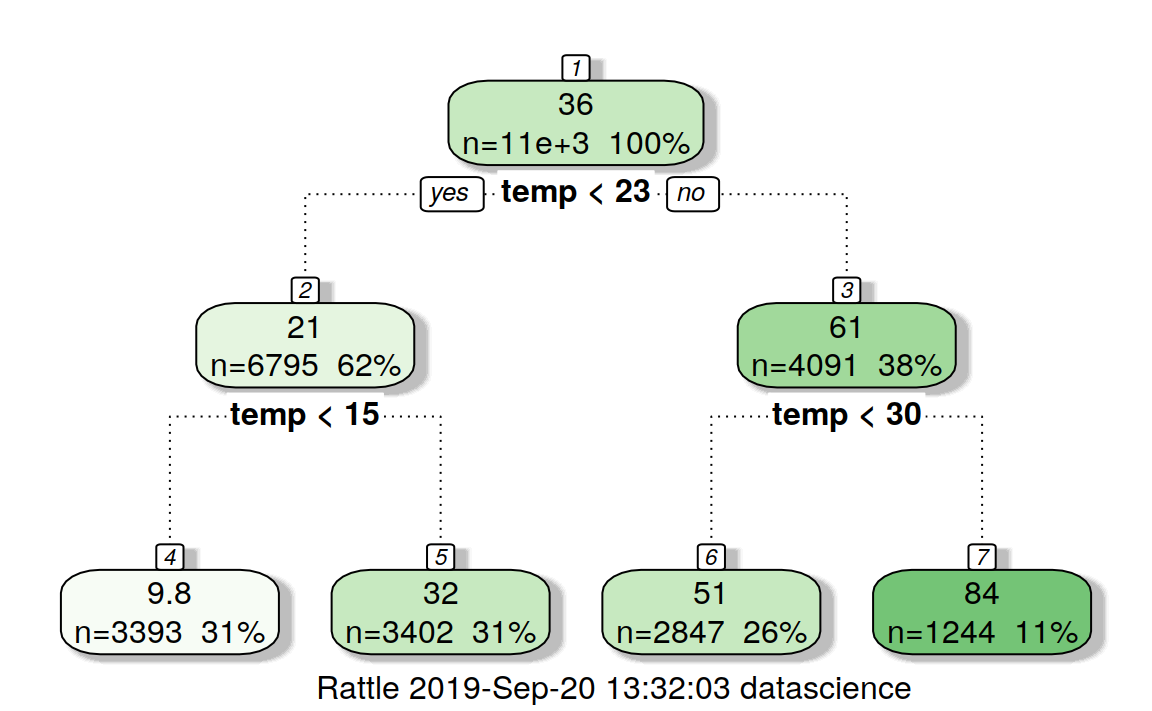
\includegraphics[width=0.7\linewidth]{meta_110b-PCA-Principal_Component_Methods_in_R_files/figure-latex/unnamed-chunk-42-1} \end{center}

\hypertarget{graph-customization}{%
\section{Graph customization}\label{graph-customization}}

Note that, fviz\_pca\_ind() and fviz\_pca\_var() and related functions are wrapper around the core function fviz() {[}in factoextra{]}. fviz() is a wrapper around the function ggscatter() {[}in ggpubr{]}. Therefore, further arguments, to be passed to the function fviz() and ggscatter(), can be specified in fviz\_pca\_ind() and fviz\_pca\_var().

Here, we present some of these additional arguments to customize the PCA graph of variables and individuals.

\hypertarget{dimensions}{%
\subsection{Dimensions}\label{dimensions}}

By default, variables/individuals are represented on dimensions 1 and 2. If you want to visualize them on dimensions 2 and 3, for example, you should specify the argument axes = c(2, 3).

\begin{Shaded}
\begin{Highlighting}[]
\CommentTok{# Variables on dimensions 2 and 3}
\KeywordTok{fviz_pca_var}\NormalTok{(res.pca, }\DataTypeTok{axes =} \KeywordTok{c}\NormalTok{(}\DecValTok{2}\NormalTok{, }\DecValTok{3}\NormalTok{))}
\CommentTok{# Individuals on dimensions 2 and 3}
\KeywordTok{fviz_pca_ind}\NormalTok{(res.pca, }\DataTypeTok{axes =} \KeywordTok{c}\NormalTok{(}\DecValTok{2}\NormalTok{, }\DecValTok{3}\NormalTok{))}
\end{Highlighting}
\end{Shaded}

\begin{center}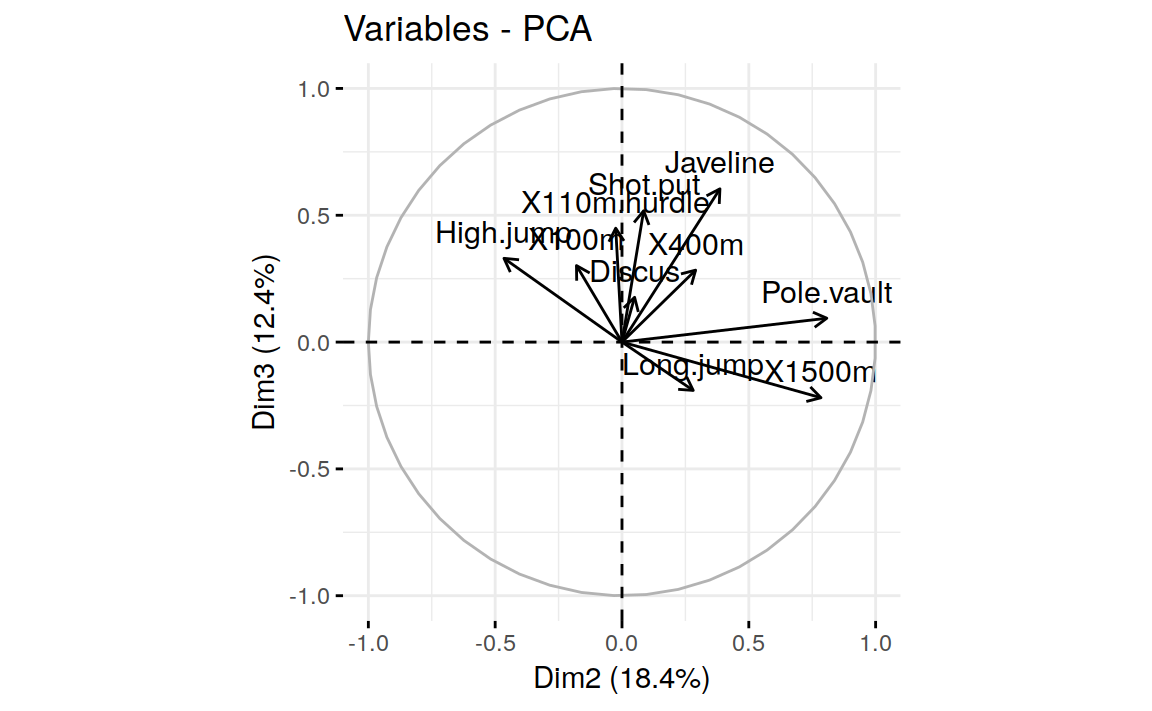
\includegraphics[width=0.7\linewidth]{meta_110b-PCA-Principal_Component_Methods_in_R_files/figure-latex/unnamed-chunk-43-1} 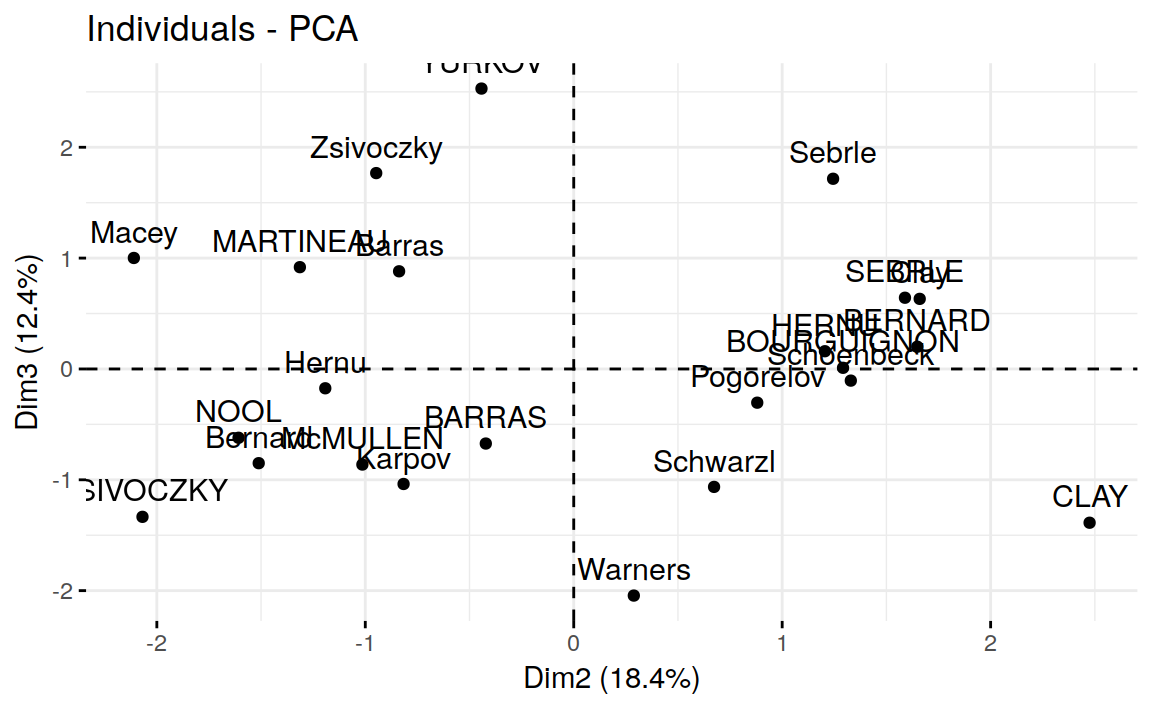
\includegraphics[width=0.7\linewidth]{meta_110b-PCA-Principal_Component_Methods_in_R_files/figure-latex/unnamed-chunk-43-2} \end{center}

Plot elements: point, text, arrow
The argument geom (for geometry) and derivatives are used to specify the geometry elements or graphical elements to be used for plotting.

\begin{enumerate}
\def\labelenumi{\arabic{enumi}.}
\tightlist
\item
  geom.var: a text specifying the geometry to be used for plotting variables. Allowed values are the combination of c(``point'', ``arrow'', ``text'').
\end{enumerate}

\begin{itemize}
\tightlist
\item
  Use geom.var = ``point'', to show only points;
\item
  Use geom.var = ``text'' to show only text labels;
\item
  Use geom.var = c(``point'', ``text'') to show both points and text labels
\item
  Use geom.var = c(``arrow'', ``text'') to show arrows and labels (default).
\end{itemize}

For example, type this:

\begin{Shaded}
\begin{Highlighting}[]
\CommentTok{# Show variable points and text labels}
\KeywordTok{fviz_pca_var}\NormalTok{(res.pca, }\DataTypeTok{geom.var =} \KeywordTok{c}\NormalTok{(}\StringTok{"point"}\NormalTok{, }\StringTok{"text"}\NormalTok{))}
\end{Highlighting}
\end{Shaded}

\begin{center}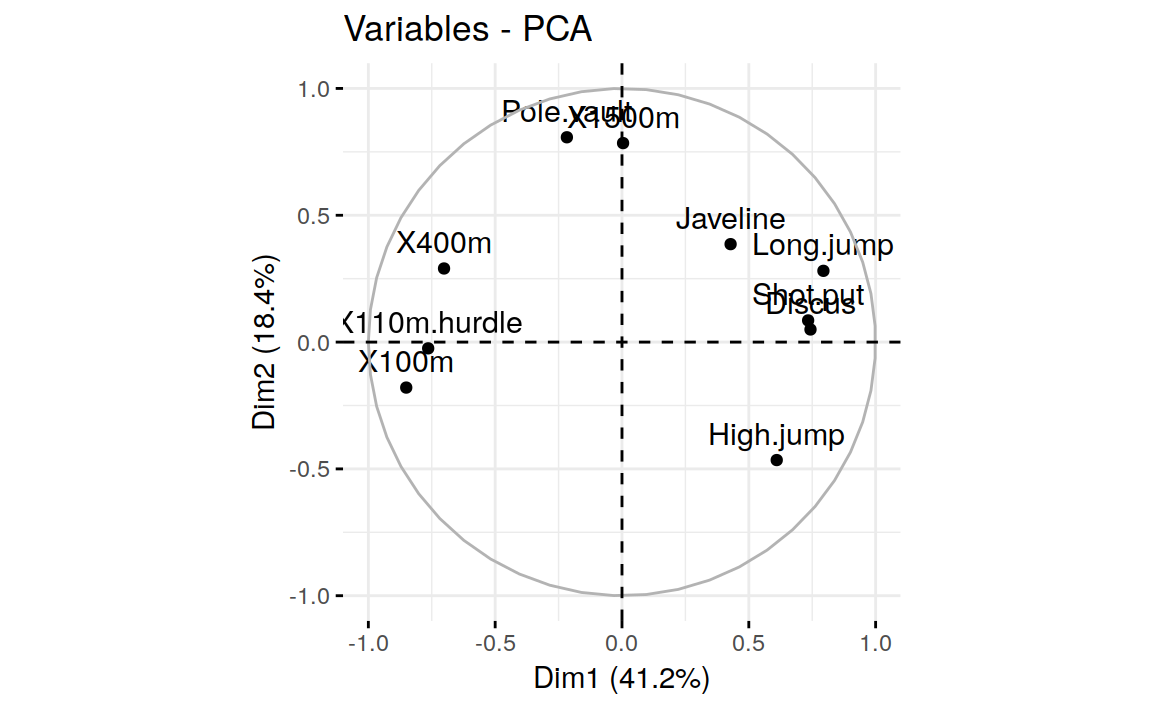
\includegraphics[width=0.7\linewidth]{meta_110b-PCA-Principal_Component_Methods_in_R_files/figure-latex/unnamed-chunk-44-1} \end{center}

\begin{Shaded}
\begin{Highlighting}[]
\CommentTok{# Show individuals text labels only}
\KeywordTok{fviz_pca_ind}\NormalTok{(res.pca, }\DataTypeTok{geom.ind =}  \StringTok{"text"}\NormalTok{)}
\end{Highlighting}
\end{Shaded}

\begin{center}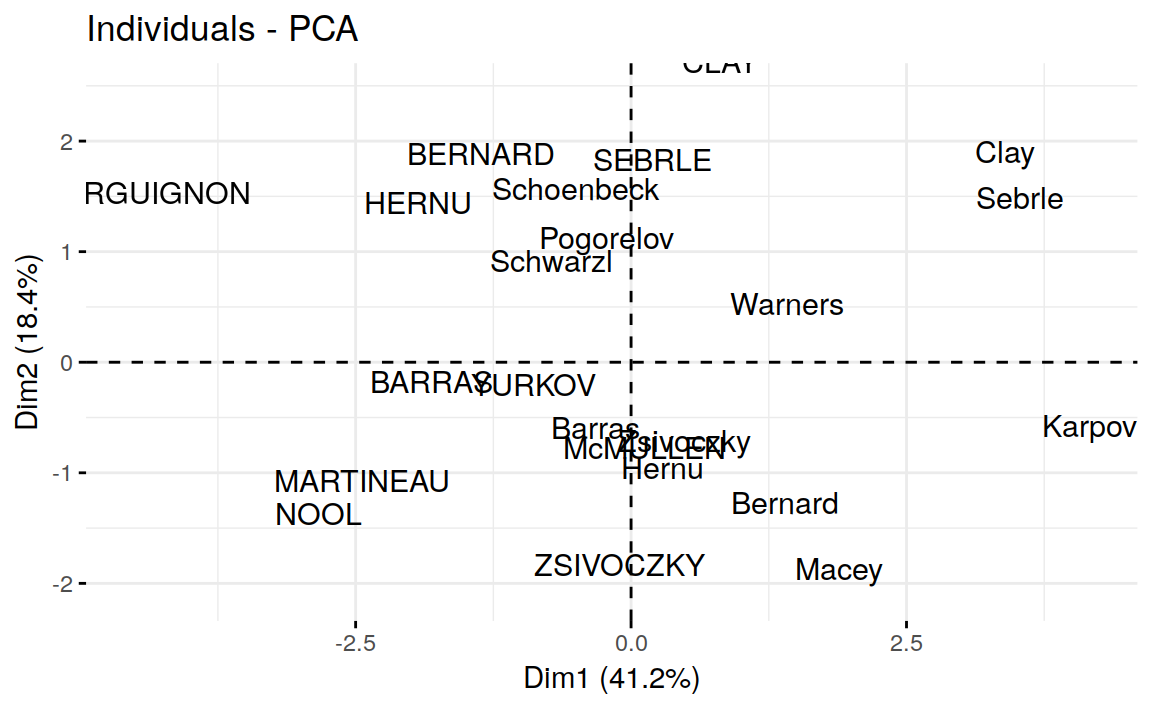
\includegraphics[width=0.7\linewidth]{meta_110b-PCA-Principal_Component_Methods_in_R_files/figure-latex/unnamed-chunk-45-1} \end{center}

\hypertarget{size-and-shape-of-plot-elements}{%
\section{Size and shape of plot elements}\label{size-and-shape-of-plot-elements}}

\begin{Shaded}
\begin{Highlighting}[]
\CommentTok{# Change the size of arrows an labels}
\KeywordTok{fviz_pca_var}\NormalTok{(res.pca, }\DataTypeTok{arrowsize =} \DecValTok{1}\NormalTok{, }\DataTypeTok{labelsize =} \DecValTok{5}\NormalTok{, }
             \DataTypeTok{repel =} \OtherTok{TRUE}\NormalTok{)}
\CommentTok{# Change points size, shape and fill color}
\CommentTok{# Change labelsize}
\KeywordTok{fviz_pca_ind}\NormalTok{(res.pca, }
             \DataTypeTok{pointsize =} \DecValTok{3}\NormalTok{, }\DataTypeTok{pointshape =} \DecValTok{21}\NormalTok{, }\DataTypeTok{fill =} \StringTok{"lightblue"}\NormalTok{,}
             \DataTypeTok{labelsize =} \DecValTok{5}\NormalTok{, }\DataTypeTok{repel =} \OtherTok{TRUE}\NormalTok{)}
\end{Highlighting}
\end{Shaded}

\begin{center}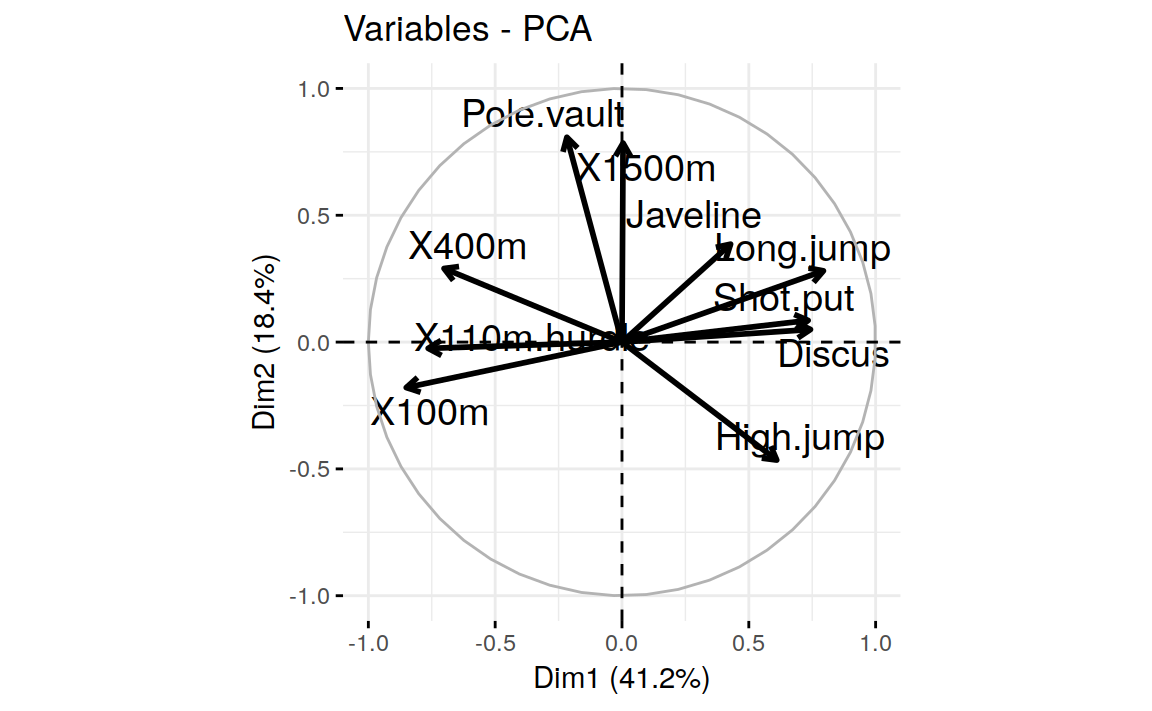
\includegraphics[width=0.7\linewidth]{meta_110b-PCA-Principal_Component_Methods_in_R_files/figure-latex/unnamed-chunk-46-1} 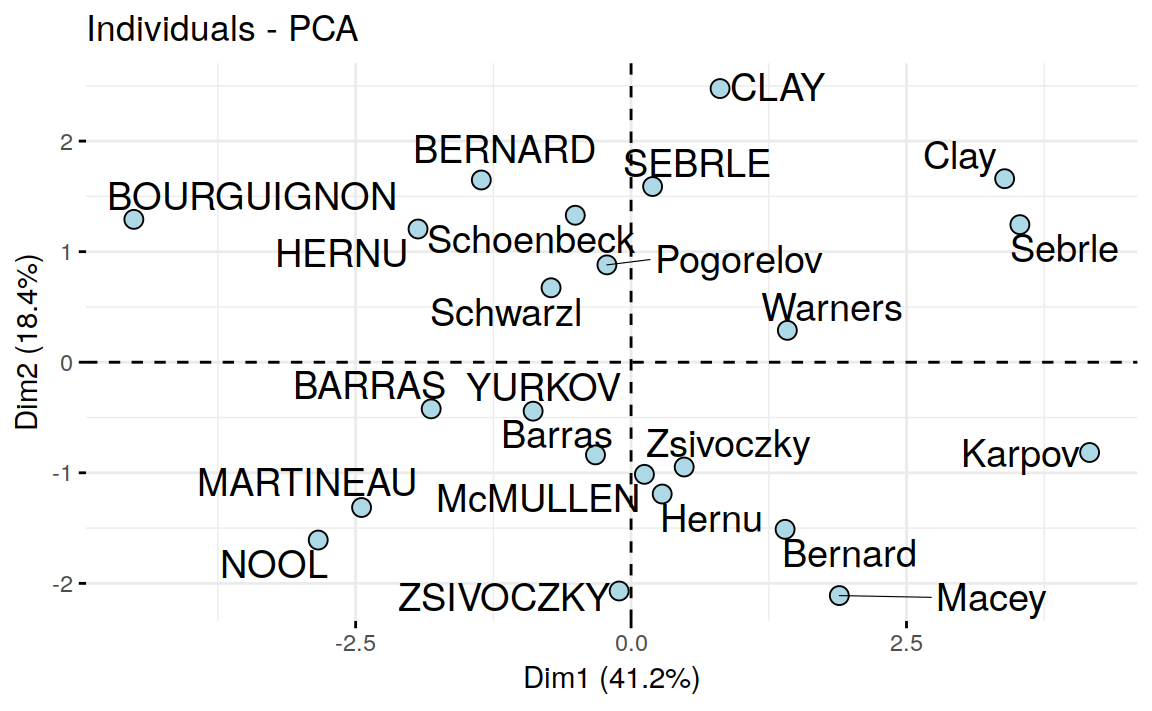
\includegraphics[width=0.7\linewidth]{meta_110b-PCA-Principal_Component_Methods_in_R_files/figure-latex/unnamed-chunk-46-2} \end{center}

\hypertarget{ellipses}{%
\section{Ellipses}\label{ellipses}}

\begin{Shaded}
\begin{Highlighting}[]
\CommentTok{# Add confidence ellipses}
\KeywordTok{fviz_pca_ind}\NormalTok{(iris.pca, }\DataTypeTok{geom.ind =} \StringTok{"point"}\NormalTok{, }
             \DataTypeTok{col.ind =}\NormalTok{ iris}\OperatorTok{$}\NormalTok{Species, }\CommentTok{# color by groups}
             \DataTypeTok{palette =} \KeywordTok{c}\NormalTok{(}\StringTok{"#00AFBB"}\NormalTok{, }\StringTok{"#E7B800"}\NormalTok{, }\StringTok{"#FC4E07"}\NormalTok{),}
             \DataTypeTok{addEllipses =} \OtherTok{TRUE}\NormalTok{, }\DataTypeTok{ellipse.type =} \StringTok{"confidence"}\NormalTok{,}
             \DataTypeTok{legend.title =} \StringTok{"Groups"}
\NormalTok{             )}
\CommentTok{# Convex hull}
\KeywordTok{fviz_pca_ind}\NormalTok{(iris.pca, }\DataTypeTok{geom.ind =} \StringTok{"point"}\NormalTok{,}
             \DataTypeTok{col.ind =}\NormalTok{ iris}\OperatorTok{$}\NormalTok{Species, }\CommentTok{# color by groups}
             \DataTypeTok{palette =} \KeywordTok{c}\NormalTok{(}\StringTok{"#00AFBB"}\NormalTok{, }\StringTok{"#E7B800"}\NormalTok{, }\StringTok{"#FC4E07"}\NormalTok{),}
             \DataTypeTok{addEllipses =} \OtherTok{TRUE}\NormalTok{, }\DataTypeTok{ellipse.type =} \StringTok{"convex"}\NormalTok{,}
             \DataTypeTok{legend.title =} \StringTok{"Groups"}
\NormalTok{             )}
\end{Highlighting}
\end{Shaded}

\begin{center}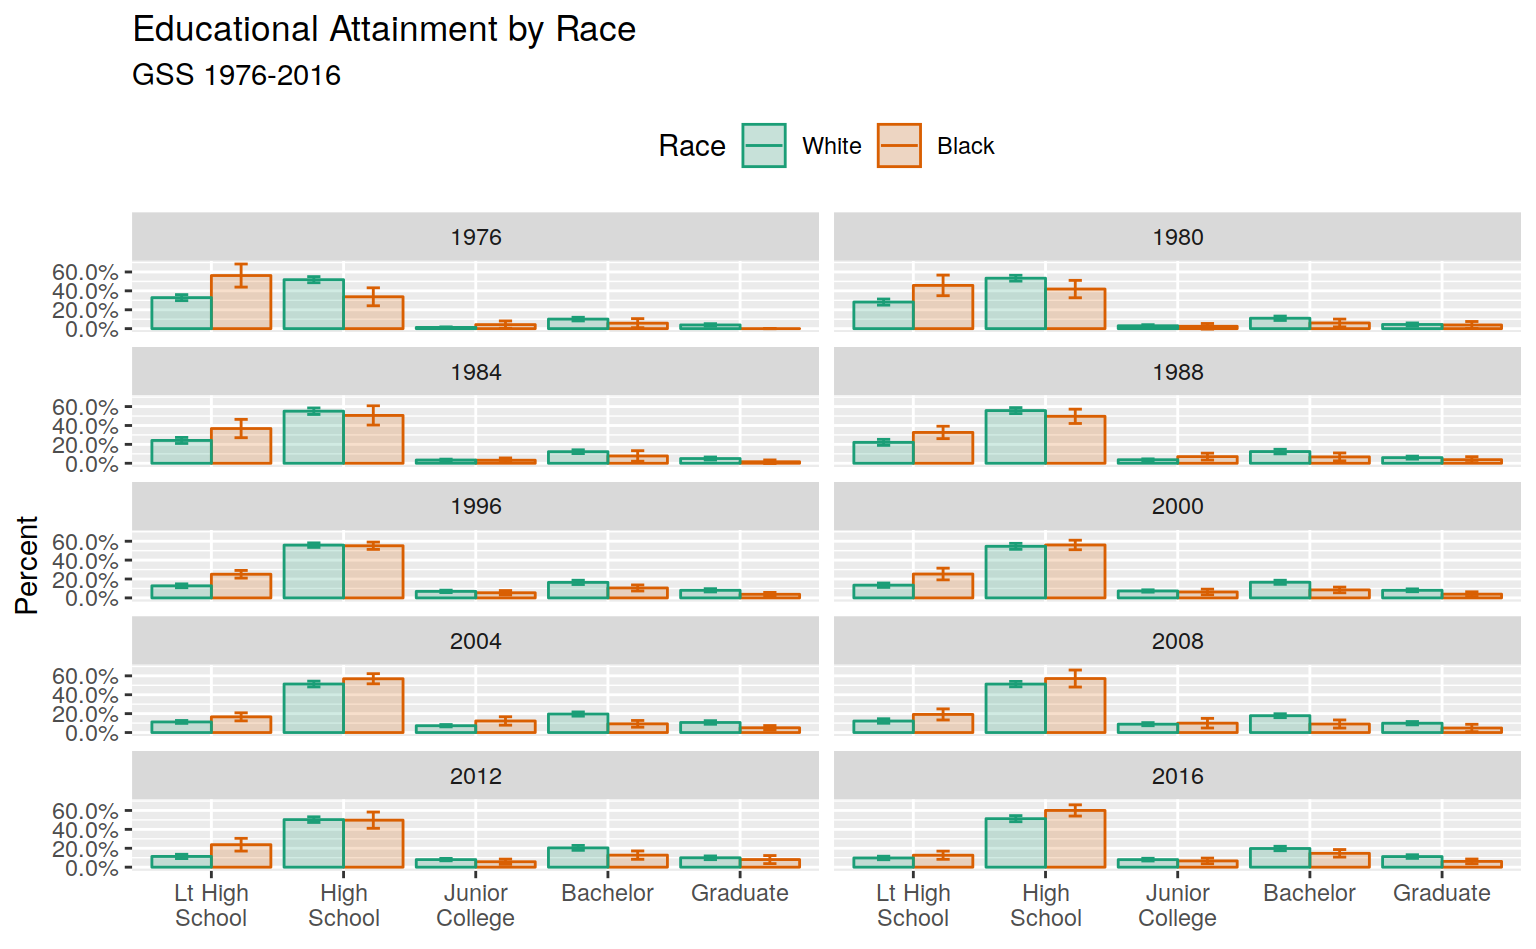
\includegraphics[width=0.7\linewidth]{meta_110b-PCA-Principal_Component_Methods_in_R_files/figure-latex/unnamed-chunk-47-1} 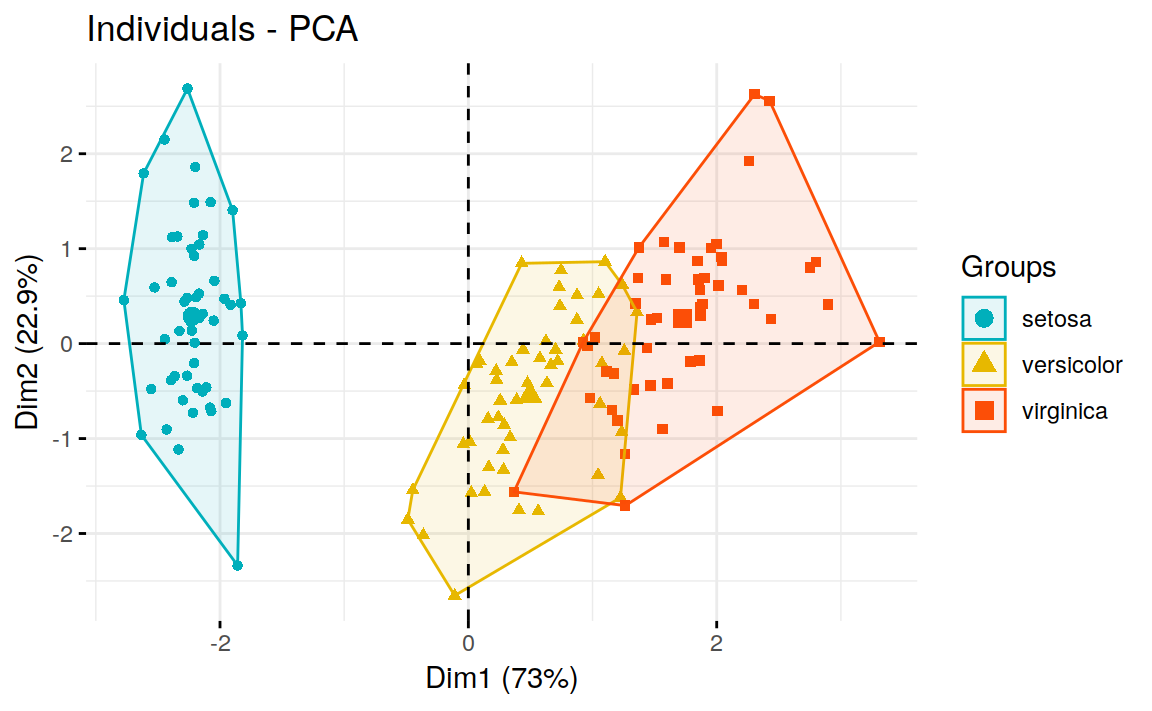
\includegraphics[width=0.7\linewidth]{meta_110b-PCA-Principal_Component_Methods_in_R_files/figure-latex/unnamed-chunk-47-2} \end{center}

\hypertarget{group-mean-points}{%
\section{Group mean points}\label{group-mean-points}}

When coloring individuals by groups (section \citet{ref}(color-ind-by-groups)), the mean points of groups (barycenters) are also displayed by default.

To remove the mean points, use the argument mean.point = FALSE.

\begin{Shaded}
\begin{Highlighting}[]
\KeywordTok{fviz_pca_ind}\NormalTok{(iris.pca,}
             \DataTypeTok{geom.ind =} \StringTok{"point"}\NormalTok{, }\CommentTok{# show points only (but not "text")}
             \DataTypeTok{group.ind =}\NormalTok{ iris}\OperatorTok{$}\NormalTok{Species, }\CommentTok{# color by groups}
             \DataTypeTok{legend.title =} \StringTok{"Groups"}\NormalTok{,}
             \DataTypeTok{mean.point =} \OtherTok{FALSE}\NormalTok{)}
\end{Highlighting}
\end{Shaded}

\begin{center}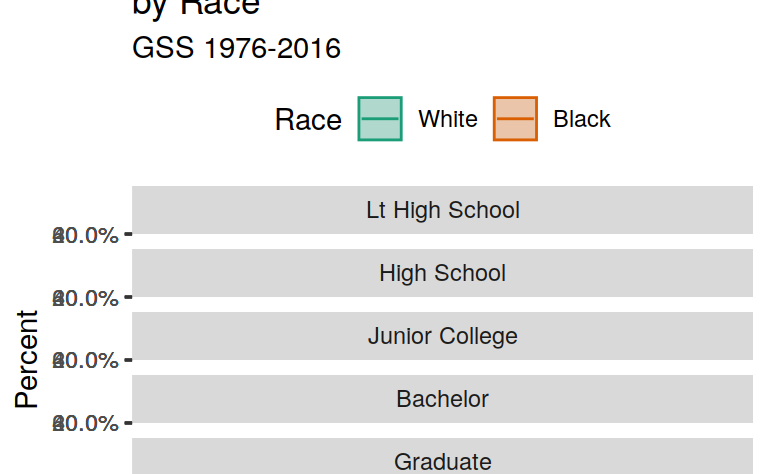
\includegraphics[width=0.7\linewidth]{meta_110b-PCA-Principal_Component_Methods_in_R_files/figure-latex/unnamed-chunk-48-1} \end{center}

\hypertarget{axis-lines}{%
\section{Axis lines}\label{axis-lines}}

\begin{Shaded}
\begin{Highlighting}[]
\KeywordTok{fviz_pca_var}\NormalTok{(res.pca, }\DataTypeTok{axes.linetype =} \StringTok{"blank"}\NormalTok{)}
\end{Highlighting}
\end{Shaded}

\begin{center}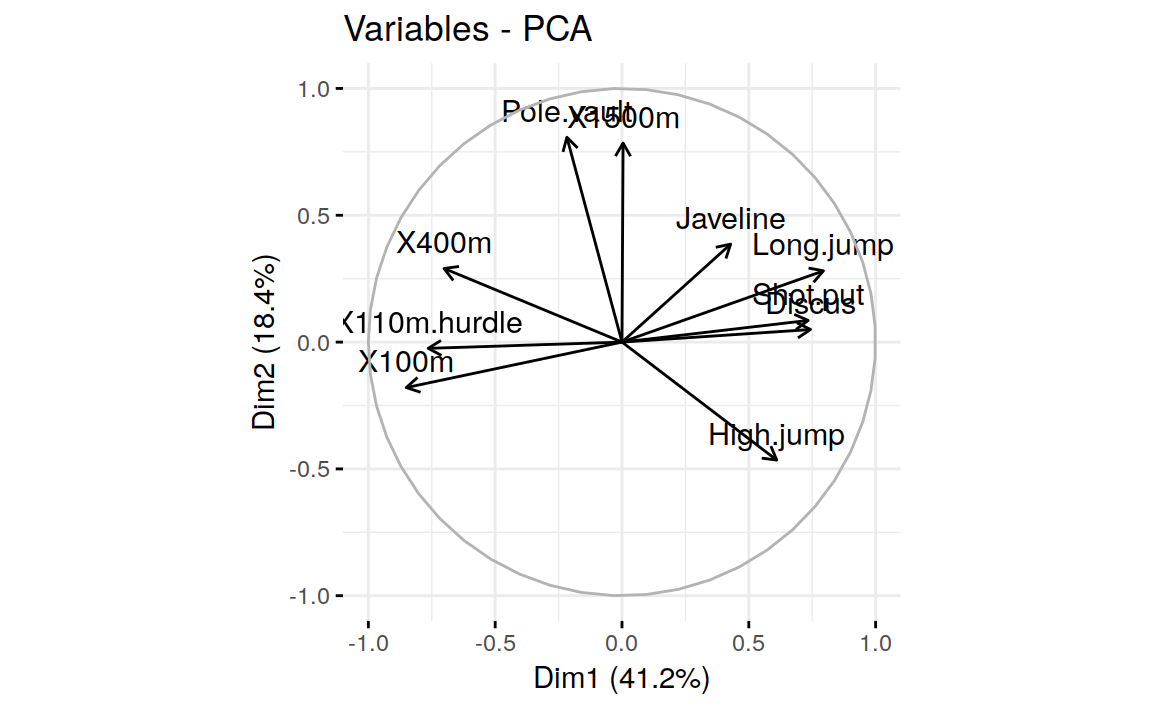
\includegraphics[width=0.7\linewidth]{meta_110b-PCA-Principal_Component_Methods_in_R_files/figure-latex/unnamed-chunk-49-1} \end{center}

\hypertarget{graphical-parameters}{%
\section{Graphical parameters}\label{graphical-parameters}}

To change easily the graphical of any ggplots, you can use the function ggpar() {[}ggpubr package{]}

\begin{Shaded}
\begin{Highlighting}[]
\NormalTok{ind.p <-}\StringTok{ }\KeywordTok{fviz_pca_ind}\NormalTok{(iris.pca, }\DataTypeTok{geom =} \StringTok{"point"}\NormalTok{, }\DataTypeTok{col.ind =}\NormalTok{ iris}\OperatorTok{$}\NormalTok{Species)}
\NormalTok{ggpubr}\OperatorTok{::}\KeywordTok{ggpar}\NormalTok{(ind.p,}
              \DataTypeTok{title =} \StringTok{"Principal Component Analysis"}\NormalTok{,}
              \DataTypeTok{subtitle =} \StringTok{"Iris data set"}\NormalTok{,}
              \DataTypeTok{caption =} \StringTok{"Source: factoextra"}\NormalTok{,}
              \DataTypeTok{xlab =} \StringTok{"PC1"}\NormalTok{, }\DataTypeTok{ylab =} \StringTok{"PC2"}\NormalTok{,}
              \DataTypeTok{legend.title =} \StringTok{"Species"}\NormalTok{, }\DataTypeTok{legend.position =} \StringTok{"top"}\NormalTok{,}
              \DataTypeTok{ggtheme =} \KeywordTok{theme_gray}\NormalTok{(), }\DataTypeTok{palette =} \StringTok{"jco"}
\NormalTok{              )}
\end{Highlighting}
\end{Shaded}

\begin{center}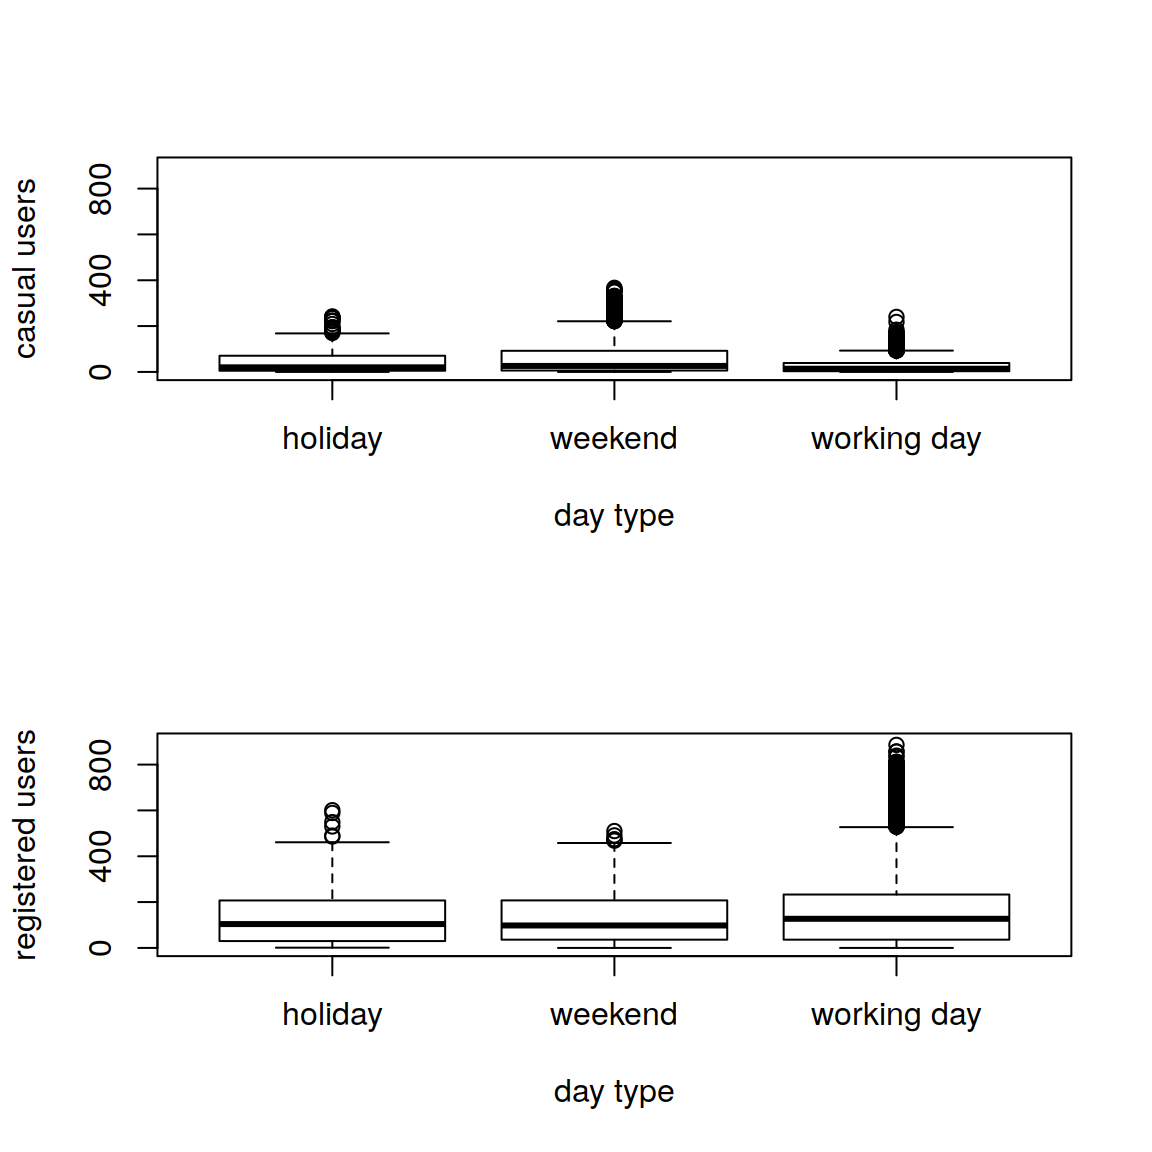
\includegraphics[width=0.7\linewidth]{meta_110b-PCA-Principal_Component_Methods_in_R_files/figure-latex/unnamed-chunk-50-1} \end{center}

\hypertarget{biplot}{%
\section{Biplot}\label{biplot}}

To make a simple biplot of individuals and variables, type this:

\begin{Shaded}
\begin{Highlighting}[]
\KeywordTok{fviz_pca_biplot}\NormalTok{(res.pca, }\DataTypeTok{repel =} \OtherTok{TRUE}\NormalTok{,}
                \DataTypeTok{col.var =} \StringTok{"#2E9FDF"}\NormalTok{, }\CommentTok{# Variables color}
                \DataTypeTok{col.ind =} \StringTok{"#696969"}  \CommentTok{# Individuals color}
\NormalTok{                )}
\end{Highlighting}
\end{Shaded}

\begin{center}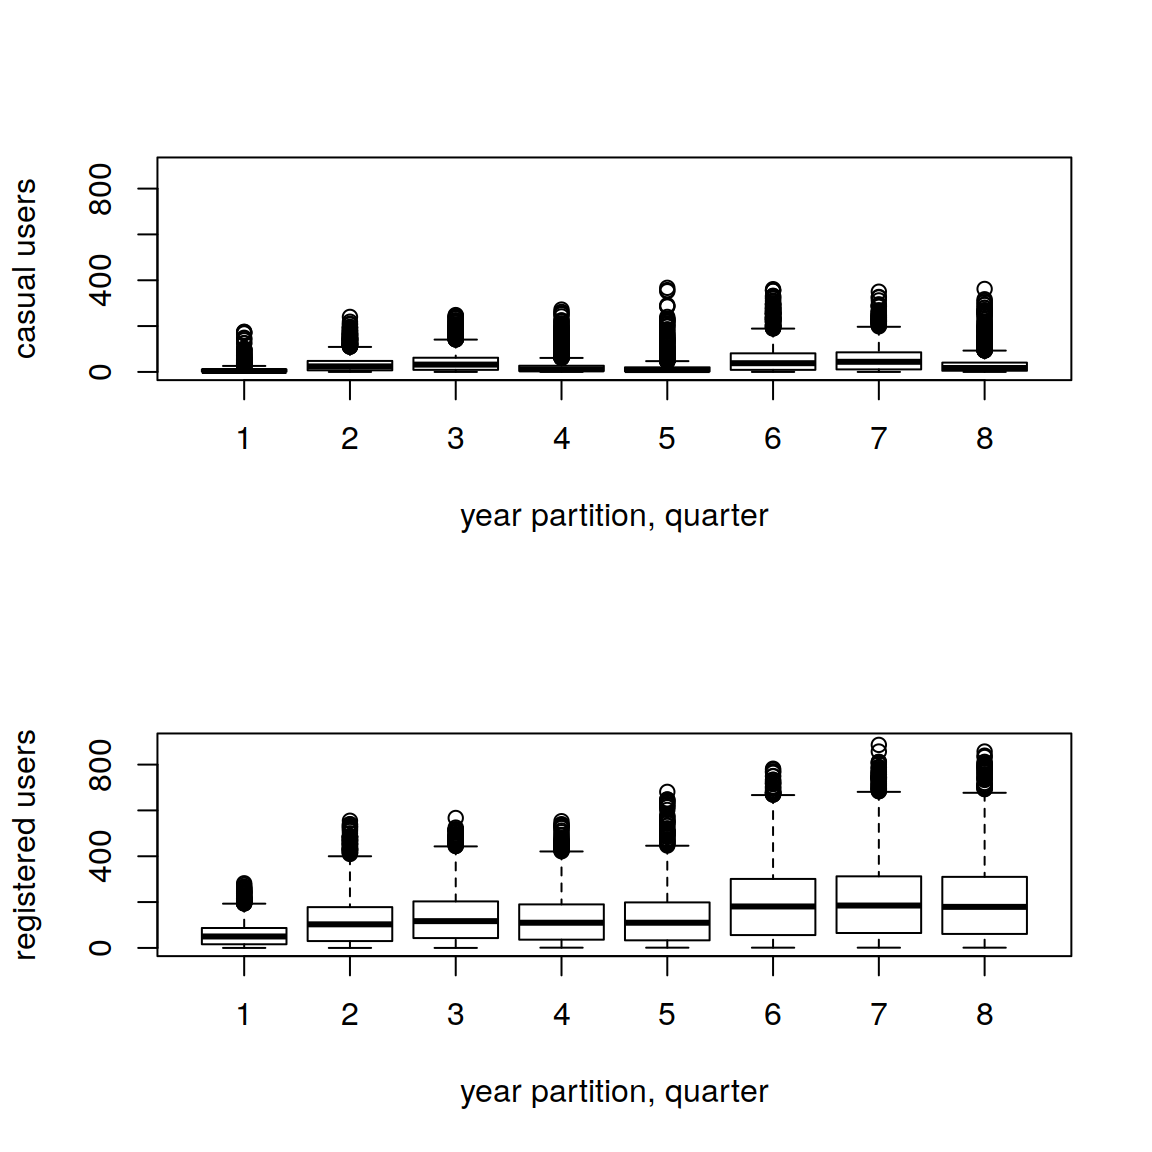
\includegraphics[width=0.7\linewidth]{meta_110b-PCA-Principal_Component_Methods_in_R_files/figure-latex/unnamed-chunk-51-1} \end{center}

\begin{quote}
Note that, the biplot might be only useful when there is a low number of variables and individuals in the data set; otherwise the final plot would be unreadable.
\end{quote}

\begin{quote}
Note also that, the coordinate of individuals and variables are not constructed on the same space. Therefore, in the biplot, you should mainly focus on the direction of variables but not on their absolute positions on the plot.
\end{quote}

\begin{quote}
Roughly speaking a biplot can be interpreted as follow:
* an individual that is on the same side of a given variable has a high value for this variable;
* an individual that is on the opposite side of a given variable has a low value for this variable.
\end{quote}

\begin{Shaded}
\begin{Highlighting}[]
\KeywordTok{fviz_pca_biplot}\NormalTok{(iris.pca, }
                \DataTypeTok{col.ind =}\NormalTok{ iris}\OperatorTok{$}\NormalTok{Species, }\DataTypeTok{palette =} \StringTok{"jco"}\NormalTok{, }
                \DataTypeTok{addEllipses =} \OtherTok{TRUE}\NormalTok{, }\DataTypeTok{label =} \StringTok{"var"}\NormalTok{,}
                \DataTypeTok{col.var =} \StringTok{"black"}\NormalTok{, }\DataTypeTok{repel =} \OtherTok{TRUE}\NormalTok{,}
                \DataTypeTok{legend.title =} \StringTok{"Species"}\NormalTok{) }
\end{Highlighting}
\end{Shaded}

\begin{center}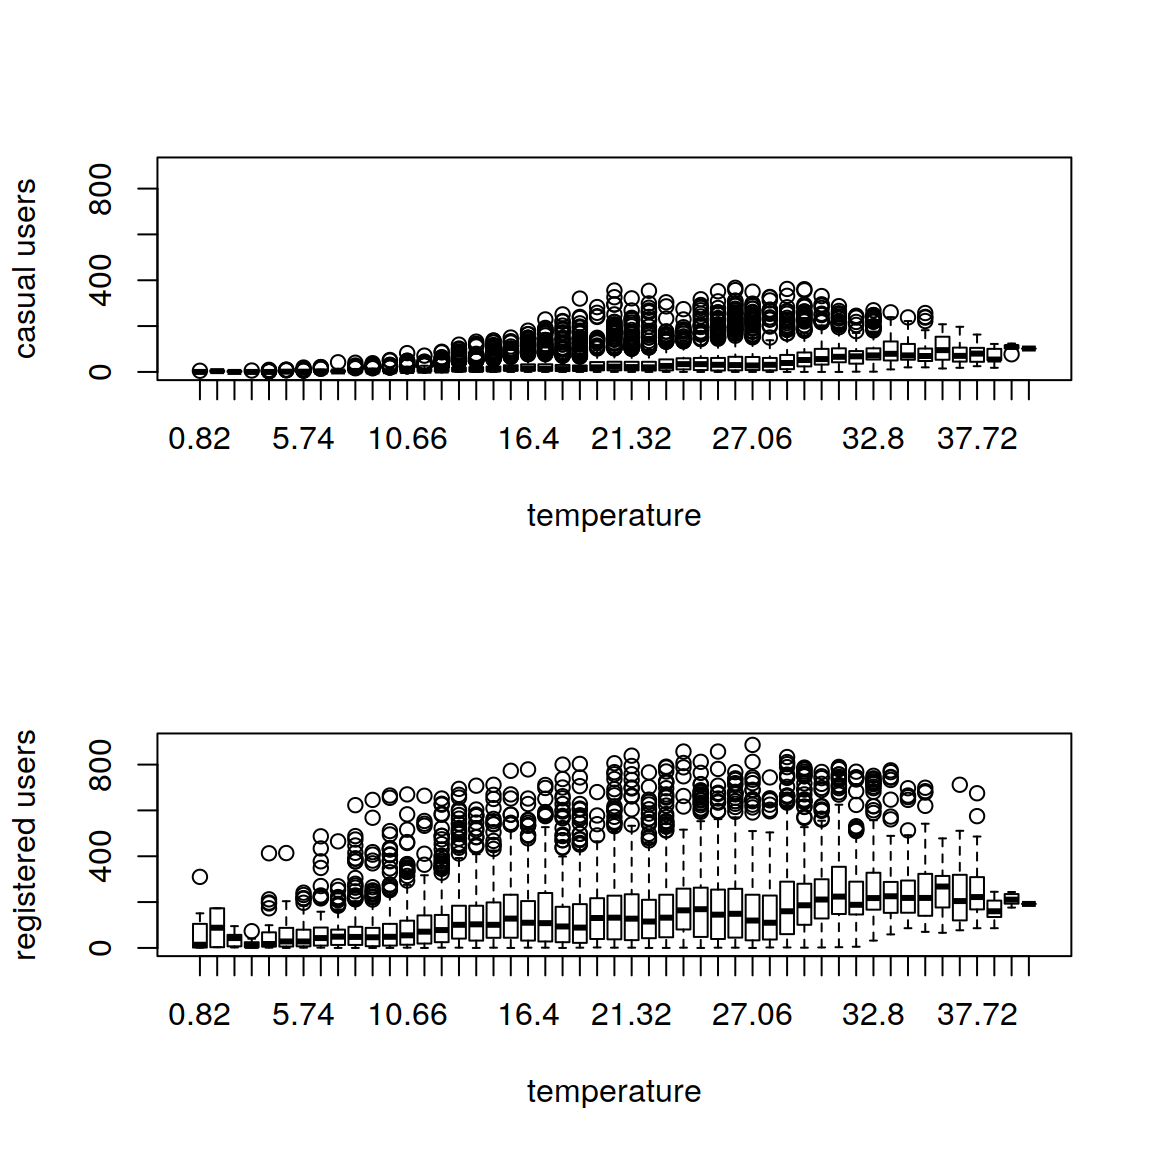
\includegraphics[width=0.7\linewidth]{meta_110b-PCA-Principal_Component_Methods_in_R_files/figure-latex/unnamed-chunk-52-1} \end{center}

In the following example, we want to color both individuals and variables by groups. The trick is to use pointshape = 21 for individual points. This particular point shape can be filled by a color using the argument fill.ind. The border line color of individual points is set to ``black'' using col.ind. To color variable by groups, the argument col.var will be used.

To customize individuals and variable colors, we use the helper functions fill\_palette() and color\_palette() {[}in ggpubr package{]}.

\begin{Shaded}
\begin{Highlighting}[]
\KeywordTok{fviz_pca_biplot}\NormalTok{(iris.pca, }
                \CommentTok{# Fill individuals by groups}
                \DataTypeTok{geom.ind =} \StringTok{"point"}\NormalTok{,}
                \DataTypeTok{pointshape =} \DecValTok{21}\NormalTok{,}
                \DataTypeTok{pointsize =} \FloatTok{2.5}\NormalTok{,}
                \DataTypeTok{fill.ind =}\NormalTok{ iris}\OperatorTok{$}\NormalTok{Species,}
                \DataTypeTok{col.ind =} \StringTok{"black"}\NormalTok{,}
                \CommentTok{# Color variable by groups}
                \DataTypeTok{col.var =} \KeywordTok{factor}\NormalTok{(}\KeywordTok{c}\NormalTok{(}\StringTok{"sepal"}\NormalTok{, }\StringTok{"sepal"}\NormalTok{, }\StringTok{"petal"}\NormalTok{, }\StringTok{"petal"}\NormalTok{)),}
                
                \DataTypeTok{legend.title =} \KeywordTok{list}\NormalTok{(}\DataTypeTok{fill =} \StringTok{"Species"}\NormalTok{, }\DataTypeTok{color =} \StringTok{"Clusters"}\NormalTok{),}
                \DataTypeTok{repel =} \OtherTok{TRUE}        \CommentTok{# Avoid label overplotting}
\NormalTok{             )}\OperatorTok{+}
\StringTok{  }\NormalTok{ggpubr}\OperatorTok{::}\KeywordTok{fill_palette}\NormalTok{(}\StringTok{"jco"}\NormalTok{)}\OperatorTok{+}\StringTok{      }\CommentTok{# Indiviual fill color}
\StringTok{  }\NormalTok{ggpubr}\OperatorTok{::}\KeywordTok{color_palette}\NormalTok{(}\StringTok{"npg"}\NormalTok{)      }\CommentTok{# Variable colors}
\end{Highlighting}
\end{Shaded}

\begin{center}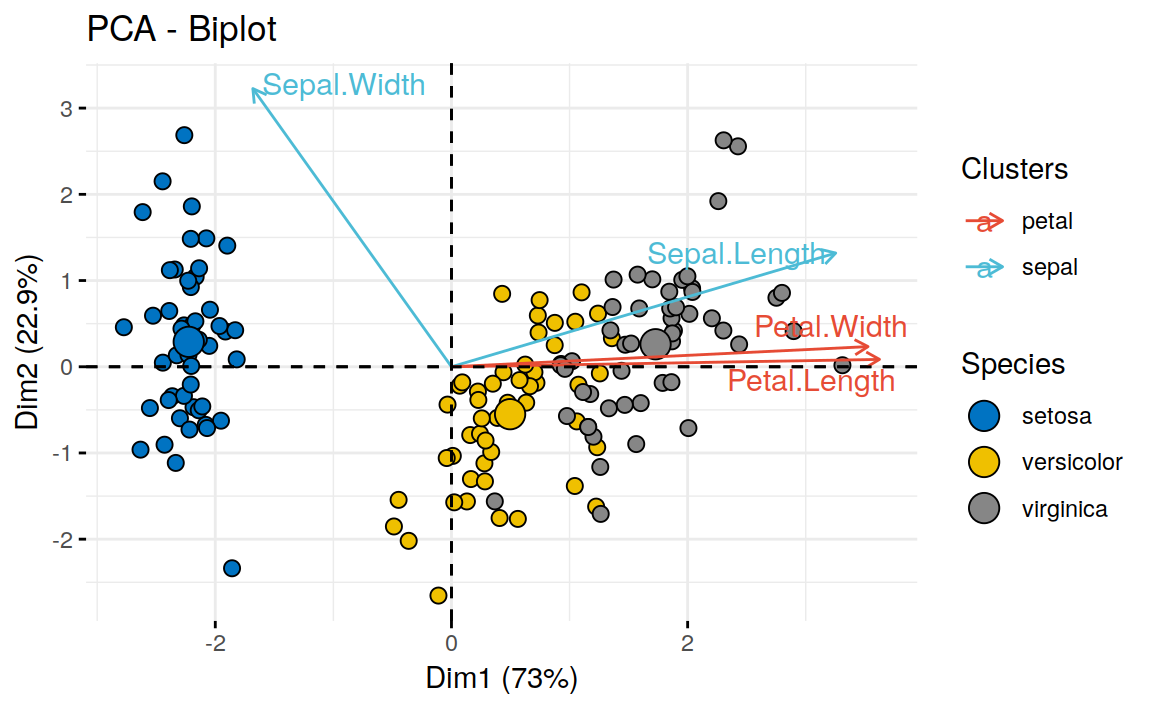
\includegraphics[width=0.7\linewidth]{meta_110b-PCA-Principal_Component_Methods_in_R_files/figure-latex/unnamed-chunk-53-1} \end{center}

Another complex example is to color individuals by groups (discrete color) and variables by their contributions to the principal components (gradient colors). Additionally, we'll change the transparency of variables by their contributions using the argument alpha.var.

\begin{Shaded}
\begin{Highlighting}[]
\KeywordTok{fviz_pca_biplot}\NormalTok{(iris.pca, }
                \CommentTok{# Individuals}
                \DataTypeTok{geom.ind =} \StringTok{"point"}\NormalTok{,}
                \DataTypeTok{fill.ind =}\NormalTok{ iris}\OperatorTok{$}\NormalTok{Species, }\DataTypeTok{col.ind =} \StringTok{"black"}\NormalTok{,}
                \DataTypeTok{pointshape =} \DecValTok{21}\NormalTok{, }\DataTypeTok{pointsize =} \DecValTok{2}\NormalTok{,}
                \DataTypeTok{palette =} \StringTok{"jco"}\NormalTok{,}
                \DataTypeTok{addEllipses =} \OtherTok{TRUE}\NormalTok{,}
                \CommentTok{# Variables}
                \DataTypeTok{alpha.var =}\StringTok{"contrib"}\NormalTok{, }\DataTypeTok{col.var =} \StringTok{"contrib"}\NormalTok{,}
                \DataTypeTok{gradient.cols =} \StringTok{"RdYlBu"}\NormalTok{,}
                
                \DataTypeTok{legend.title =} \KeywordTok{list}\NormalTok{(}\DataTypeTok{fill =} \StringTok{"Species"}\NormalTok{, }\DataTypeTok{color =} \StringTok{"Contrib"}\NormalTok{,}
                                    \DataTypeTok{alpha =} \StringTok{"Contrib"}\NormalTok{)}
\NormalTok{                )}
\end{Highlighting}
\end{Shaded}

\begin{center}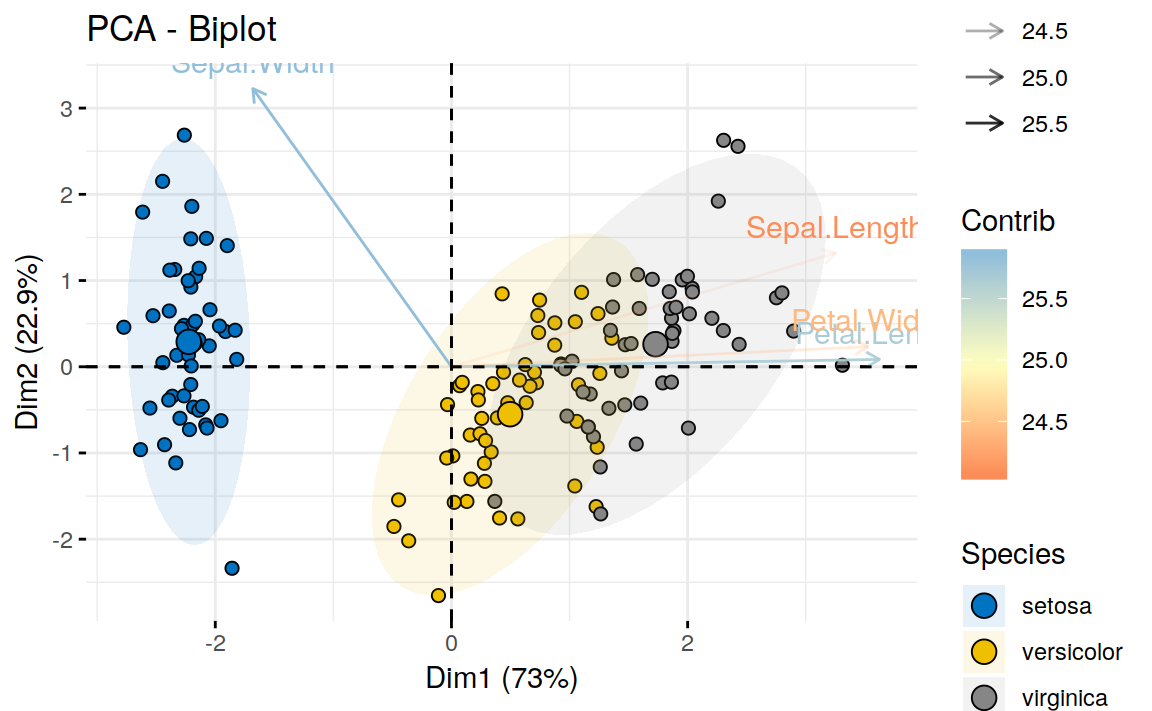
\includegraphics[width=0.7\linewidth]{meta_110b-PCA-Principal_Component_Methods_in_R_files/figure-latex/unnamed-chunk-54-1} \end{center}

\hypertarget{supplementary-elements}{%
\section{Supplementary elements}\label{supplementary-elements}}

Definition and types
As described above (section \citet{ref}(pca-data-format)), the decathlon2 data sets contain supplementary continuous variables (quanti.sup, columns 11:12), supplementary qualitative variables (quali.sup, column 13) and supplementary individuals (ind.sup, rows 24:27).

Supplementary variables and individuals are not used for the determination of the principal components. Their coordinates are predicted using only the information provided by the performed principal component analysis on active variables/individuals.

Specification in PCA
To specify supplementary individuals and variables, the function PCA() can be used as follow:

\begin{Shaded}
\begin{Highlighting}[]
\NormalTok{res.pca <-}\StringTok{ }\KeywordTok{PCA}\NormalTok{(decathlon2, }\DataTypeTok{ind.sup =} \DecValTok{24}\OperatorTok{:}\DecValTok{27}\NormalTok{, }
               \DataTypeTok{quanti.sup =} \DecValTok{11}\OperatorTok{:}\DecValTok{12}\NormalTok{, }\DataTypeTok{quali.sup =} \DecValTok{13}\NormalTok{, }\DataTypeTok{graph=}\OtherTok{FALSE}\NormalTok{)}
\end{Highlighting}
\end{Shaded}

\hypertarget{quantitative-variables-1}{%
\section{Quantitative variables}\label{quantitative-variables-1}}

Predicted results (coordinates, correlation and cos2) for the supplementary quantitative variables:

\begin{Shaded}
\begin{Highlighting}[]
\NormalTok{res.pca}\OperatorTok{$}\NormalTok{quanti.sup}
\CommentTok{#> $coord}
\CommentTok{#>         Dim.1   Dim.2  Dim.3   Dim.4   Dim.5}
\CommentTok{#> Rank   -0.701 -0.2452 -0.183  0.0558 -0.0738}
\CommentTok{#> Points  0.964  0.0777  0.158 -0.1662 -0.0311}
\CommentTok{#> }
\CommentTok{#> $cor}
\CommentTok{#>         Dim.1   Dim.2  Dim.3   Dim.4   Dim.5}
\CommentTok{#> Rank   -0.701 -0.2452 -0.183  0.0558 -0.0738}
\CommentTok{#> Points  0.964  0.0777  0.158 -0.1662 -0.0311}
\CommentTok{#> }
\CommentTok{#> $cos2}
\CommentTok{#>        Dim.1   Dim.2  Dim.3   Dim.4   Dim.5}
\CommentTok{#> Rank   0.492 0.06012 0.0336 0.00311 0.00545}
\CommentTok{#> Points 0.929 0.00603 0.0250 0.02763 0.00097}
\end{Highlighting}
\end{Shaded}

Visualize all variables (active and supplementary ones):

\begin{Shaded}
\begin{Highlighting}[]
\KeywordTok{fviz_pca_var}\NormalTok{(res.pca)}
\end{Highlighting}
\end{Shaded}

\begin{center}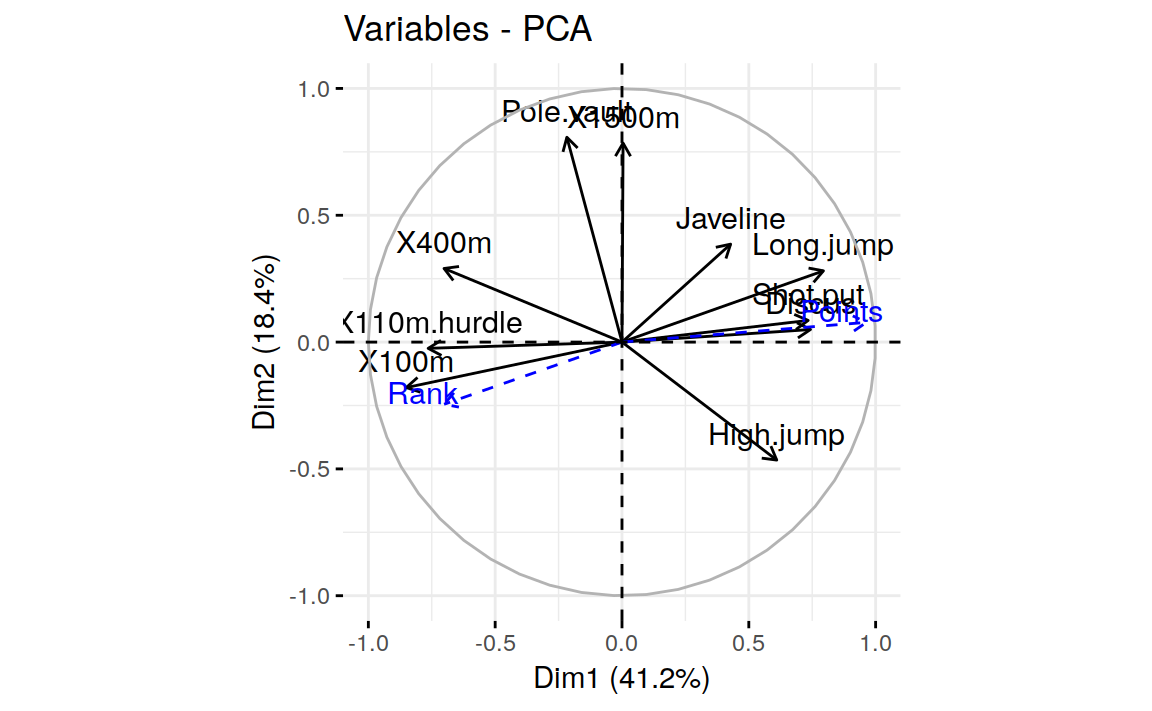
\includegraphics[width=0.7\linewidth]{meta_110b-PCA-Principal_Component_Methods_in_R_files/figure-latex/unnamed-chunk-57-1} \end{center}

\begin{quote}
Note that, by default, supplementary quantitative variables are shown in blue color and dashed lines.
\end{quote}

Further arguments to customize the plot:

\begin{Shaded}
\begin{Highlighting}[]
\CommentTok{# Change color of variables}
\KeywordTok{fviz_pca_var}\NormalTok{(res.pca,}
             \DataTypeTok{col.var =} \StringTok{"black"}\NormalTok{,     }\CommentTok{# Active variables}
             \DataTypeTok{col.quanti.sup =} \StringTok{"red"} \CommentTok{# Suppl. quantitative variables}
\NormalTok{             )}
\CommentTok{# Hide active variables on the plot, }
\CommentTok{# show only supplementary variables}
\KeywordTok{fviz_pca_var}\NormalTok{(res.pca, }\DataTypeTok{invisible =} \StringTok{"var"}\NormalTok{)}
\CommentTok{# Hide supplementary variables}
\KeywordTok{fviz_pca_var}\NormalTok{(res.pca, }\DataTypeTok{invisible =} \StringTok{"quanti.sup"}\NormalTok{)}
\end{Highlighting}
\end{Shaded}

\begin{center}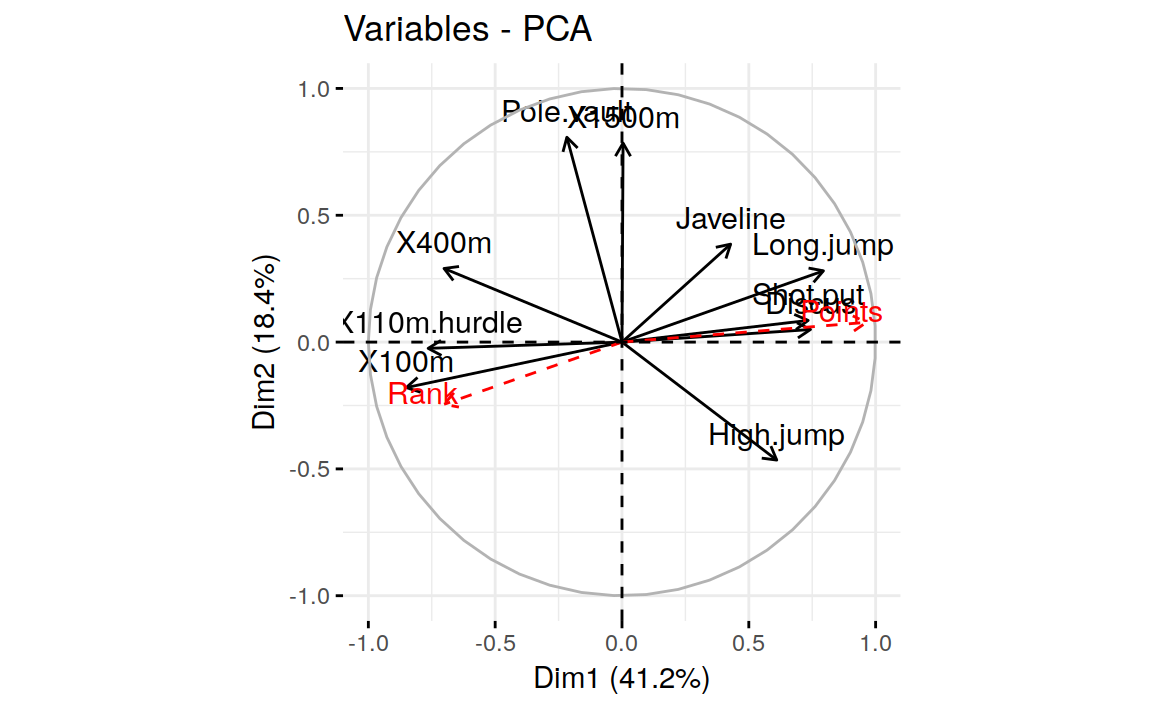
\includegraphics[width=0.7\linewidth]{meta_110b-PCA-Principal_Component_Methods_in_R_files/figure-latex/unnamed-chunk-58-1} 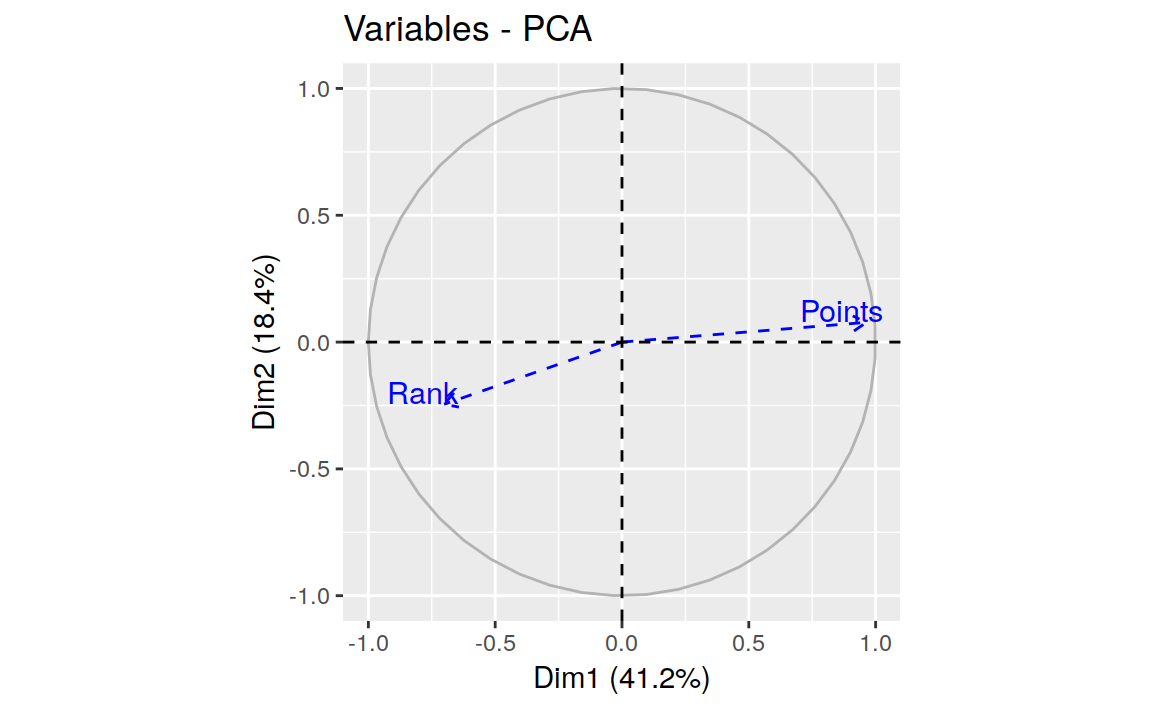
\includegraphics[width=0.7\linewidth]{meta_110b-PCA-Principal_Component_Methods_in_R_files/figure-latex/unnamed-chunk-58-2} 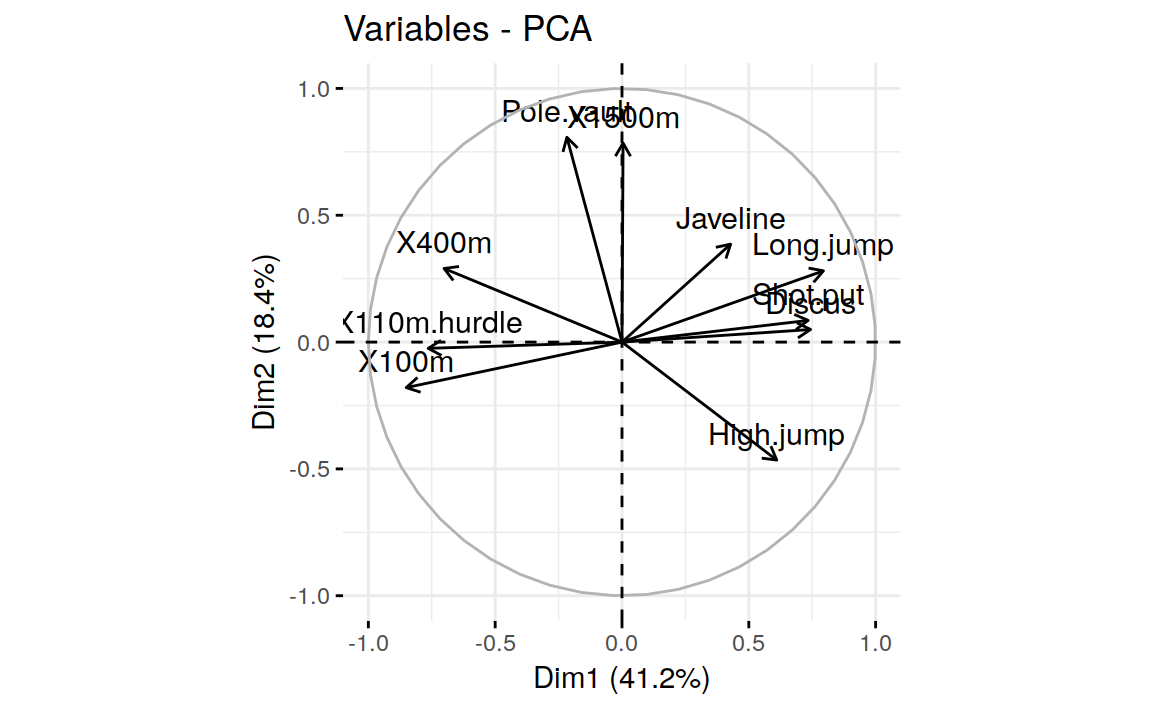
\includegraphics[width=0.7\linewidth]{meta_110b-PCA-Principal_Component_Methods_in_R_files/figure-latex/unnamed-chunk-58-3} \end{center}

\begin{quote}
Using the fviz\_pca\_var(), the quantitative supplementary variables are displayed automatically on the correlation circle plot. Note that, you can add the quanti.sup variables manually, using the fviz\_add() function, for further customization. An example is shown below.
\end{quote}

\begin{Shaded}
\begin{Highlighting}[]
\CommentTok{# Plot of active variables}
\NormalTok{p <-}\StringTok{ }\KeywordTok{fviz_pca_var}\NormalTok{(res.pca, }\DataTypeTok{invisible =} \StringTok{"quanti.sup"}\NormalTok{)}
\CommentTok{# Add supplementary active variables}
\KeywordTok{fviz_add}\NormalTok{(p, res.pca}\OperatorTok{$}\NormalTok{quanti.sup}\OperatorTok{$}\NormalTok{coord, }
         \DataTypeTok{geom =} \KeywordTok{c}\NormalTok{(}\StringTok{"arrow"}\NormalTok{, }\StringTok{"text"}\NormalTok{), }
         \DataTypeTok{color =} \StringTok{"red"}\NormalTok{)}
\end{Highlighting}
\end{Shaded}

\begin{center}\includegraphics[width=0.7\linewidth]{meta_110b-PCA-Principal_Component_Methods_in_R_files/figure-latex/unnamed-chunk-59-1} \end{center}

\hypertarget{individuals}{%
\section{Individuals}\label{individuals}}

Predicted results for the supplementary individuals (ind.sup):

\begin{Shaded}
\begin{Highlighting}[]
\NormalTok{res.pca}\OperatorTok{$}\NormalTok{ind.sup}
\CommentTok{#> $coord}
\CommentTok{#>          Dim.1   Dim.2  Dim.3  Dim.4   Dim.5}
\CommentTok{#> KARPOV   0.795  0.7795 -1.633  1.724 -0.7507}
\CommentTok{#> WARNERS -0.386 -0.1216 -1.739 -0.706 -0.0323}
\CommentTok{#> Nool    -0.559  1.9775 -0.483 -2.278 -0.2546}
\CommentTok{#> Drews   -1.109  0.0174 -3.049 -1.534 -0.3264}
\CommentTok{#> }
\CommentTok{#> $cos2}
\CommentTok{#>          Dim.1    Dim.2  Dim.3  Dim.4    Dim.5}
\CommentTok{#> KARPOV  0.0510 4.91e-02 0.2155 0.2403 0.045549}
\CommentTok{#> WARNERS 0.0242 2.40e-03 0.4904 0.0809 0.000169}
\CommentTok{#> Nool    0.0290 3.62e-01 0.0216 0.4811 0.006008}
\CommentTok{#> Drews   0.0921 2.27e-05 0.6956 0.1762 0.007974}
\CommentTok{#> }
\CommentTok{#> $dist}
\CommentTok{#>  KARPOV WARNERS    Nool   Drews }
\CommentTok{#>    3.52    2.48    3.28    3.66}
\end{Highlighting}
\end{Shaded}

Visualize all individuals (active and supplementary ones). On the graph, you can add also the supplementary qualitative variables (quali.sup), which coordinates is accessible using res.pca\(quali.supp\)coord.

\begin{Shaded}
\begin{Highlighting}[]
\NormalTok{p <-}\StringTok{ }\KeywordTok{fviz_pca_ind}\NormalTok{(res.pca, }\DataTypeTok{col.ind.sup =} \StringTok{"blue"}\NormalTok{, }\DataTypeTok{repel =} \OtherTok{TRUE}\NormalTok{)}
\NormalTok{p <-}\StringTok{ }\KeywordTok{fviz_add}\NormalTok{(p, res.pca}\OperatorTok{$}\NormalTok{quali.sup}\OperatorTok{$}\NormalTok{coord, }\DataTypeTok{color =} \StringTok{"red"}\NormalTok{)}
\NormalTok{p}
\end{Highlighting}
\end{Shaded}

\begin{center}\includegraphics[width=0.7\linewidth]{meta_110b-PCA-Principal_Component_Methods_in_R_files/figure-latex/unnamed-chunk-61-1} \end{center}

\begin{quote}
Supplementary individuals are shown in blue. The levels of the supplementary qualitative variable are shown in red color.
\end{quote}

\hypertarget{qualitative-variables}{%
\section{Qualitative variables}\label{qualitative-variables}}

In the previous section, we showed that you can add the supplementary qualitative variables on individuals plot using fviz\_add().

Note that, the supplementary qualitative variables can be also used for coloring individuals by groups. This can help to interpret the data. The data sets decathlon2 contain a supplementary qualitative variable at columns 13 corresponding to the type of competitions.

The results concerning the supplementary qualitative variable are:

\begin{Shaded}
\begin{Highlighting}[]
\NormalTok{res.pca}\OperatorTok{$}\NormalTok{quali}
\CommentTok{#> $coord}
\CommentTok{#>          Dim.1  Dim.2   Dim.3  Dim.4  Dim.5}
\CommentTok{#> Decastar -1.34  0.122 -0.0379  0.181  0.134}
\CommentTok{#> OlympicG  1.23 -0.112  0.0347 -0.166 -0.123}
\CommentTok{#> }
\CommentTok{#> $cos2}
\CommentTok{#>          Dim.1   Dim.2   Dim.3  Dim.4   Dim.5}
\CommentTok{#> Decastar 0.905 0.00744 0.00072 0.0164 0.00905}
\CommentTok{#> OlympicG 0.905 0.00744 0.00072 0.0164 0.00905}
\CommentTok{#> }
\CommentTok{#> $v.test}
\CommentTok{#>          Dim.1  Dim.2  Dim.3  Dim.4 Dim.5}
\CommentTok{#> Decastar -2.97  0.403 -0.153  0.897  0.72}
\CommentTok{#> OlympicG  2.97 -0.403  0.153 -0.897 -0.72}
\CommentTok{#> }
\CommentTok{#> $dist}
\CommentTok{#> Decastar OlympicG }
\CommentTok{#>     1.41     1.29 }
\CommentTok{#> }
\CommentTok{#> $eta2}
\CommentTok{#>             Dim.1  Dim.2   Dim.3  Dim.4  Dim.5}
\CommentTok{#> Competition 0.401 0.0074 0.00106 0.0366 0.0236}
\end{Highlighting}
\end{Shaded}

To color individuals by a supplementary qualitative variable, the argument habillage is used to specify the index of the supplementary qualitative variable. Historically, this argument name comes from the FactoMineR package. It's a french word meaning ``dressing'' in english. To keep consistency between FactoMineR and factoextra, we decided to keep the same argument name

\begin{Shaded}
\begin{Highlighting}[]
\KeywordTok{fviz_pca_ind}\NormalTok{(res.pca, }\DataTypeTok{habillage =} \DecValTok{13}\NormalTok{,}
             \DataTypeTok{addEllipses =}\OtherTok{TRUE}\NormalTok{, }\DataTypeTok{ellipse.type =} \StringTok{"confidence"}\NormalTok{,}
             \DataTypeTok{palette =} \StringTok{"jco"}\NormalTok{, }\DataTypeTok{repel =} \OtherTok{TRUE}\NormalTok{) }
\end{Highlighting}
\end{Shaded}

\begin{center}\includegraphics[width=0.7\linewidth]{meta_110b-PCA-Principal_Component_Methods_in_R_files/figure-latex/unnamed-chunk-63-1} \end{center}

\begin{quote}
Recall that, to remove the mean points of groups, specify the argument mean.point = FALSE.
\end{quote}

\hypertarget{filtering-results}{%
\section{Filtering results}\label{filtering-results}}

If you have many individuals/variable, it's possible to visualize only some of them using the arguments select.ind and select.var.

\begin{Shaded}
\begin{Highlighting}[]
\CommentTok{# Visualize variable with cos2 >= 0.6}
\KeywordTok{fviz_pca_var}\NormalTok{(res.pca, }\DataTypeTok{select.var =} \KeywordTok{list}\NormalTok{(}\DataTypeTok{cos2 =} \FloatTok{0.6}\NormalTok{))}
\CommentTok{# Top 5 active variables with the highest cos2}
\KeywordTok{fviz_pca_var}\NormalTok{(res.pca, }\DataTypeTok{select.var=} \KeywordTok{list}\NormalTok{(}\DataTypeTok{cos2 =} \DecValTok{5}\NormalTok{))}
\CommentTok{# Select by names}
\NormalTok{name <-}\StringTok{ }\KeywordTok{list}\NormalTok{(}\DataTypeTok{name =} \KeywordTok{c}\NormalTok{(}\StringTok{"Long.jump"}\NormalTok{, }\StringTok{"High.jump"}\NormalTok{, }\StringTok{"X100m"}\NormalTok{))}
\KeywordTok{fviz_pca_var}\NormalTok{(res.pca, }\DataTypeTok{select.var =}\NormalTok{ name)}
\CommentTok{# top 5 contributing individuals and variable}
\KeywordTok{fviz_pca_biplot}\NormalTok{(res.pca, }\DataTypeTok{select.ind =} \KeywordTok{list}\NormalTok{(}\DataTypeTok{contrib =} \DecValTok{5}\NormalTok{), }
               \DataTypeTok{select.var =} \KeywordTok{list}\NormalTok{(}\DataTypeTok{contrib =} \DecValTok{5}\NormalTok{),}
               \DataTypeTok{ggtheme =} \KeywordTok{theme_minimal}\NormalTok{())}
\end{Highlighting}
\end{Shaded}

\begin{center}\includegraphics[width=0.7\linewidth]{meta_110b-PCA-Principal_Component_Methods_in_R_files/figure-latex/unnamed-chunk-64-1} \includegraphics[width=0.7\linewidth]{meta_110b-PCA-Principal_Component_Methods_in_R_files/figure-latex/unnamed-chunk-64-2} \includegraphics[width=0.7\linewidth]{meta_110b-PCA-Principal_Component_Methods_in_R_files/figure-latex/unnamed-chunk-64-3} \includegraphics[width=0.7\linewidth]{meta_110b-PCA-Principal_Component_Methods_in_R_files/figure-latex/unnamed-chunk-64-4} \end{center}

\begin{quote}
When the selection is done according to the contribution values, supplementary individuals/variables are not shown because they don't contribute to the construction of the axes.
\end{quote}

\hypertarget{exporting-results}{%
\section{Exporting results}\label{exporting-results}}

Export plots to PDF/PNG files
The factoextra package produces a ggplot2-based graphs. To save any ggplots, the standard R code is as follow:

\begin{verbatim}
# Print the plot to a pdf file
pdf("myplot.pdf")
print(myplot)
dev.off()
\end{verbatim}

In the following examples, we'll show you how to save the different graphs into pdf or png files.

The first step is to create the plots you want as an R object:

\begin{Shaded}
\begin{Highlighting}[]
\CommentTok{# Scree plot}
\NormalTok{scree.plot <-}\StringTok{ }\KeywordTok{fviz_eig}\NormalTok{(res.pca)}
\CommentTok{# Plot of individuals}
\NormalTok{ind.plot <-}\StringTok{ }\KeywordTok{fviz_pca_ind}\NormalTok{(res.pca)}
\CommentTok{# Plot of variables}
\NormalTok{var.plot <-}\StringTok{ }\KeywordTok{fviz_pca_var}\NormalTok{(res.pca)}
\end{Highlighting}
\end{Shaded}

\begin{Shaded}
\begin{Highlighting}[]
\KeywordTok{pdf}\NormalTok{(}\KeywordTok{file.path}\NormalTok{(data_out_dir, }\StringTok{"PCA.pdf"}\NormalTok{))   }\CommentTok{# Create a new pdf device}
\KeywordTok{print}\NormalTok{(scree.plot)}
\KeywordTok{print}\NormalTok{(ind.plot)}
\KeywordTok{print}\NormalTok{(var.plot)}
\KeywordTok{dev.off}\NormalTok{() }\CommentTok{# Close the pdf device}
\CommentTok{#> pdf }
\CommentTok{#>   2}
\end{Highlighting}
\end{Shaded}

\begin{quote}
Note that, using the above R code will create the PDF file into your current working directory. To see the path of your current working directory, type getwd() in the R console.
\end{quote}

To print each plot to specific png file, the R code looks like this:

\begin{Shaded}
\begin{Highlighting}[]
\CommentTok{# Print scree plot to a png file}
\KeywordTok{png}\NormalTok{(}\KeywordTok{file.path}\NormalTok{(data_out_dir, }\StringTok{"pca-scree-plot.png"}\NormalTok{))}
\KeywordTok{print}\NormalTok{(scree.plot)}
\KeywordTok{dev.off}\NormalTok{()}
\CommentTok{#> pdf }
\CommentTok{#>   2}
\CommentTok{# Print individuals plot to a png file}
\KeywordTok{png}\NormalTok{(}\KeywordTok{file.path}\NormalTok{(data_out_dir, }\StringTok{"pca-variables.png"}\NormalTok{))}
\KeywordTok{print}\NormalTok{(var.plot)}
\KeywordTok{dev.off}\NormalTok{()}
\CommentTok{#> pdf }
\CommentTok{#>   2}
\CommentTok{# Print variables plot to a png file}
\KeywordTok{png}\NormalTok{(}\KeywordTok{file.path}\NormalTok{(data_out_dir, }\StringTok{"pca-individuals.png"}\NormalTok{))}
\KeywordTok{print}\NormalTok{(ind.plot)}
\KeywordTok{dev.off}\NormalTok{()}
\CommentTok{#> pdf }
\CommentTok{#>   2}
\end{Highlighting}
\end{Shaded}

Another alternative, to export ggplots, is to use the function ggexport() {[}in ggpubr package{]}. We like ggexport(), because it's very simple. With one line R code, it allows us to export individual plots to a file (pdf, eps or png) (one plot per page). It can also arrange the plots (2 plot per page, for example) before exporting them. The examples below demonstrates how to export ggplots using ggexport().

Export individual plots to a pdf file (one plot per page):

\begin{Shaded}
\begin{Highlighting}[]
\KeywordTok{library}\NormalTok{(ggpubr)}
\CommentTok{#> Loading required package: magrittr}
\KeywordTok{ggexport}\NormalTok{(}\DataTypeTok{plotlist =} \KeywordTok{list}\NormalTok{(scree.plot, ind.plot, var.plot), }
         \DataTypeTok{filename =} \KeywordTok{file.path}\NormalTok{(data_out_dir, }\StringTok{"PCA.pdf"}\NormalTok{))}
\CommentTok{#> file saved to /home/datascience/repos/machine-learning-rsuite/export/PCA.pdf}
\end{Highlighting}
\end{Shaded}

Arrange and export. Specify nrow and ncol to display multiple plots on the same page:

\begin{Shaded}
\begin{Highlighting}[]
\KeywordTok{ggexport}\NormalTok{(}\DataTypeTok{plotlist =} \KeywordTok{list}\NormalTok{(scree.plot, ind.plot, var.plot), }
         \DataTypeTok{nrow =} \DecValTok{2}\NormalTok{, }\DataTypeTok{ncol =} \DecValTok{2}\NormalTok{,}
         \DataTypeTok{filename =} \KeywordTok{file.path}\NormalTok{(data_out_dir, }\StringTok{"PCA.pdf"}\NormalTok{))}
\CommentTok{#> file saved to /home/datascience/repos/machine-learning-rsuite/export/PCA.pdf}
\end{Highlighting}
\end{Shaded}

Export plots to png files. If you specify a list of plots, then multiple png files will be automatically created to hold each plot.

\begin{Shaded}
\begin{Highlighting}[]
\KeywordTok{ggexport}\NormalTok{(}\DataTypeTok{plotlist =} \KeywordTok{list}\NormalTok{(scree.plot, ind.plot, var.plot),}
         \DataTypeTok{filename =} \KeywordTok{file.path}\NormalTok{(data_out_dir, }\StringTok{"PCA.png"}\NormalTok{))}
\CommentTok{#> [1] "/home/datascience/repos/machine-learning-rsuite/export/PCA%03d.png"}
\CommentTok{#> file saved to /home/datascience/repos/machine-learning-rsuite/export/PCA%03d.png}
\end{Highlighting}
\end{Shaded}

\hypertarget{export-results-to-txtcsv-files}{%
\section{Export results to txt/csv files}\label{export-results-to-txtcsv-files}}

All the outputs of the PCA (individuals/variables coordinates, contributions, etc) can be exported at once, into a TXT/CSV file, using the function write.infile() {[}in FactoMineR{]} package:

\begin{Shaded}
\begin{Highlighting}[]
\CommentTok{# Export into a TXT file}
\KeywordTok{write.infile}\NormalTok{(res.pca, }\KeywordTok{file.path}\NormalTok{(data_out_dir, }\StringTok{"pca.txt"}\NormalTok{), }\DataTypeTok{sep =} \StringTok{"}\CharTok{\textbackslash{}t}\StringTok{"}\NormalTok{)}
\CommentTok{# Export into a CSV file}
\KeywordTok{write.infile}\NormalTok{(res.pca, }\KeywordTok{file.path}\NormalTok{(data_out_dir, }\StringTok{"pca.csv"}\NormalTok{), }\DataTypeTok{sep =} \StringTok{";"}\NormalTok{)}
\end{Highlighting}
\end{Shaded}

\hypertarget{summary}{%
\section{Summary}\label{summary}}

In conclusion, we described how to perform and interpret principal component analysis (PCA). We computed PCA using the PCA() function {[}FactoMineR{]}. Next, we used the factoextra R package to produce ggplot2-based visualization of the PCA results.

There are other functions {[}packages{]} to compute PCA in R:

\begin{enumerate}
\def\labelenumi{\arabic{enumi}.}
\tightlist
\item
  Using prcomp() {[}stats{]}
\end{enumerate}

\begin{Shaded}
\begin{Highlighting}[]
\NormalTok{res.pca <-}\StringTok{ }\KeywordTok{prcomp}\NormalTok{(iris[, }\DecValTok{-5}\NormalTok{], }\DataTypeTok{scale. =} \OtherTok{TRUE}\NormalTok{)}
\end{Highlighting}
\end{Shaded}

\begin{Shaded}
\begin{Highlighting}[]
\NormalTok{res.pca <-}\StringTok{ }\KeywordTok{princomp}\NormalTok{(iris[, }\DecValTok{-5}\NormalTok{], }\DataTypeTok{cor =} \OtherTok{TRUE}\NormalTok{)}
\end{Highlighting}
\end{Shaded}

\begin{enumerate}
\def\labelenumi{\arabic{enumi}.}
\setcounter{enumi}{2}
\tightlist
\item
  Using dudi.pca() {[}ade4{]}
\end{enumerate}

\begin{Shaded}
\begin{Highlighting}[]
\KeywordTok{library}\NormalTok{(ade4)}
\CommentTok{#> }
\CommentTok{#> Attaching package: 'ade4'}
\CommentTok{#> The following object is masked from 'package:FactoMineR':}
\CommentTok{#> }
\CommentTok{#>     reconst}
\NormalTok{res.pca <-}\StringTok{ }\KeywordTok{dudi.pca}\NormalTok{(iris[, }\DecValTok{-5}\NormalTok{], }\DataTypeTok{scannf =} \OtherTok{FALSE}\NormalTok{, }\DataTypeTok{nf =} \DecValTok{5}\NormalTok{)}
\end{Highlighting}
\end{Shaded}

\begin{enumerate}
\def\labelenumi{\arabic{enumi}.}
\setcounter{enumi}{3}
\tightlist
\item
  Using epPCA() {[}ExPosition{]}
\end{enumerate}

\begin{Shaded}
\begin{Highlighting}[]
\KeywordTok{library}\NormalTok{(ExPosition)}
\CommentTok{#> Loading required package: prettyGraphs}
\NormalTok{res.pca <-}\StringTok{ }\KeywordTok{epPCA}\NormalTok{(iris[, }\DecValTok{-5}\NormalTok{], }\DataTypeTok{graph =} \OtherTok{FALSE}\NormalTok{)}
\end{Highlighting}
\end{Shaded}

No matter what functions you decide to use, in the list above, the factoextra package can handle the output for creating beautiful plots similar to what we described in the previous sections for FactoMineR:

\begin{Shaded}
\begin{Highlighting}[]
\KeywordTok{fviz_eig}\NormalTok{(res.pca)     }\CommentTok{# Scree plot}
\KeywordTok{fviz_pca_ind}\NormalTok{(res.pca) }\CommentTok{# Graph of individuals}
\KeywordTok{fviz_pca_var}\NormalTok{(res.pca) }\CommentTok{# Graph of variables}
\end{Highlighting}
\end{Shaded}

\begin{center}\includegraphics[width=0.7\linewidth]{meta_110b-PCA-Principal_Component_Methods_in_R_files/figure-latex/unnamed-chunk-76-1} \includegraphics[width=0.7\linewidth]{meta_110b-PCA-Principal_Component_Methods_in_R_files/figure-latex/unnamed-chunk-76-2} \includegraphics[width=0.7\linewidth]{meta_110b-PCA-Principal_Component_Methods_in_R_files/figure-latex/unnamed-chunk-76-3} \end{center}

\hypertarget{biplot-of-the-iris-data-set}{%
\chapter{Biplot of the Iris data set}\label{biplot-of-the-iris-data-set}}

\begin{Shaded}
\begin{Highlighting}[]
\CommentTok{# devtools::install_github("vqv/ggbiplot")}
\KeywordTok{library}\NormalTok{(ggbiplot)}
\CommentTok{#> Loading required package: ggplot2}
\CommentTok{#> Registered S3 methods overwritten by 'ggplot2':}
\CommentTok{#>   method         from }
\CommentTok{#>   [.quosures     rlang}
\CommentTok{#>   c.quosures     rlang}
\CommentTok{#>   print.quosures rlang}
\CommentTok{#> Loading required package: plyr}
\CommentTok{#> Loading required package: scales}
\CommentTok{#> Loading required package: grid}

\NormalTok{iris.pca <-}\StringTok{ }\KeywordTok{prcomp}\NormalTok{(iris[, }\DecValTok{1}\OperatorTok{:}\DecValTok{4}\NormalTok{], }\DataTypeTok{center =} \OtherTok{TRUE}\NormalTok{, }\DataTypeTok{scale =} \OtherTok{TRUE}\NormalTok{)}
\KeywordTok{print}\NormalTok{(iris.pca)}
\CommentTok{#> Standard deviations (1, .., p=4):}
\CommentTok{#> [1] 1.708 0.956 0.383 0.144}
\CommentTok{#> }
\CommentTok{#> Rotation (n x k) = (4 x 4):}
\CommentTok{#>                 PC1     PC2    PC3    PC4}
\CommentTok{#> Sepal.Length  0.521 -0.3774  0.720  0.261}
\CommentTok{#> Sepal.Width  -0.269 -0.9233 -0.244 -0.124}
\CommentTok{#> Petal.Length  0.580 -0.0245 -0.142 -0.801}
\CommentTok{#> Petal.Width   0.565 -0.0669 -0.634  0.524}
\end{Highlighting}
\end{Shaded}

\begin{Shaded}
\begin{Highlighting}[]
\KeywordTok{summary}\NormalTok{(iris.pca)}
\CommentTok{#> Importance of components:}
\CommentTok{#>                         PC1   PC2    PC3     PC4}
\CommentTok{#> Standard deviation     1.71 0.956 0.3831 0.14393}
\CommentTok{#> Proportion of Variance 0.73 0.229 0.0367 0.00518}
\CommentTok{#> Cumulative Proportion  0.73 0.958 0.9948 1.00000}
\end{Highlighting}
\end{Shaded}

\begin{Shaded}
\begin{Highlighting}[]
\NormalTok{g <-}\StringTok{ }\KeywordTok{ggbiplot}\NormalTok{(iris.pca,}
              \DataTypeTok{obs.scale =} \DecValTok{1}\NormalTok{,}
              \DataTypeTok{var.scale =} \DecValTok{1}\NormalTok{,}
              \DataTypeTok{groups =}\NormalTok{ iris}\OperatorTok{$}\NormalTok{Species,}
              \DataTypeTok{ellipse =} \OtherTok{TRUE}\NormalTok{,}
              \DataTypeTok{circle =} \OtherTok{TRUE}\NormalTok{) }\OperatorTok{+}
\StringTok{    }\KeywordTok{scale_color_discrete}\NormalTok{(}\DataTypeTok{name =} \StringTok{""}\NormalTok{) }\OperatorTok{+}
\StringTok{    }\KeywordTok{theme}\NormalTok{(}\DataTypeTok{legend.direction =} \StringTok{"horizontal"}\NormalTok{, }\DataTypeTok{legend.position =} \StringTok{"top"}\NormalTok{)}

\KeywordTok{print}\NormalTok{(g)}
\end{Highlighting}
\end{Shaded}

\begin{center}\includegraphics[width=0.7\linewidth]{meta_110c-PCA-Phan_2016-Introduction_To_PCA_with_examples_in_R_files/figure-latex/unnamed-chunk-4-1} \end{center}

The PC1 axis explains 0.730 of the variance, while the PC2 axis explains
0.229 of the variance.

\hypertarget{iris-underlying-principal-components}{%
\section{Iris: underlying principal components}\label{iris-underlying-principal-components}}

\begin{Shaded}
\begin{Highlighting}[]
\CommentTok{# Run PCA here with prcomp ()}
\NormalTok{iris.pca <-}\StringTok{ }\KeywordTok{prcomp}\NormalTok{(iris[, }\DecValTok{1}\OperatorTok{:}\DecValTok{4}\NormalTok{], }\DataTypeTok{center =} \OtherTok{TRUE}\NormalTok{, }\DataTypeTok{scale =} \OtherTok{TRUE}\NormalTok{)}

\KeywordTok{print}\NormalTok{(iris.pca)}
\CommentTok{#> Standard deviations (1, .., p=4):}
\CommentTok{#> [1] 1.708 0.956 0.383 0.144}
\CommentTok{#> }
\CommentTok{#> Rotation (n x k) = (4 x 4):}
\CommentTok{#>                 PC1     PC2    PC3    PC4}
\CommentTok{#> Sepal.Length  0.521 -0.3774  0.720  0.261}
\CommentTok{#> Sepal.Width  -0.269 -0.9233 -0.244 -0.124}
\CommentTok{#> Petal.Length  0.580 -0.0245 -0.142 -0.801}
\CommentTok{#> Petal.Width   0.565 -0.0669 -0.634  0.524}
\end{Highlighting}
\end{Shaded}

\begin{Shaded}
\begin{Highlighting}[]
\CommentTok{# Now, compute the new dataset aligned to the PCs by}
\CommentTok{# using the predict() function .}
\NormalTok{df.new <-}\StringTok{ }\KeywordTok{predict}\NormalTok{(iris.pca, iris[, }\DecValTok{1}\OperatorTok{:}\DecValTok{4}\NormalTok{])}
\KeywordTok{head}\NormalTok{(df.new)}
\CommentTok{#>        PC1    PC2     PC3      PC4}
\CommentTok{#> [1,] -2.26 -0.478  0.1273  0.02409}
\CommentTok{#> [2,] -2.07  0.672  0.2338  0.10266}
\CommentTok{#> [3,] -2.36  0.341 -0.0441  0.02828}
\CommentTok{#> [4,] -2.29  0.595 -0.0910 -0.06574}
\CommentTok{#> [5,] -2.38 -0.645 -0.0157 -0.03580}
\CommentTok{#> [6,] -2.07 -1.484 -0.0269  0.00659}
\end{Highlighting}
\end{Shaded}

\begin{Shaded}
\begin{Highlighting}[]
\CommentTok{# Show the PCA model’s sdev values are the square root}
\CommentTok{# of the projected variances, which are along the diagonal}
\CommentTok{# of the covariance matrix of the projected data.}
\NormalTok{iris.pca}\OperatorTok{$}\NormalTok{sdev}\OperatorTok{^}\DecValTok{2}
\CommentTok{#> [1] 2.9185 0.9140 0.1468 0.0207}
\end{Highlighting}
\end{Shaded}

\begin{Shaded}
\begin{Highlighting}[]
\CommentTok{# # Compute covariance matrix for new dataset.}
\CommentTok{# Recall that the standard deviation is the square root of the variance.}
\KeywordTok{round}\NormalTok{(}\KeywordTok{cov}\NormalTok{(df.new), }\DecValTok{5}\NormalTok{)}
\CommentTok{#>      PC1   PC2   PC3    PC4}
\CommentTok{#> PC1 2.92 0.000 0.000 0.0000}
\CommentTok{#> PC2 0.00 0.914 0.000 0.0000}
\CommentTok{#> PC3 0.00 0.000 0.147 0.0000}
\CommentTok{#> PC4 0.00 0.000 0.000 0.0207}
\end{Highlighting}
\end{Shaded}

\hypertarget{iris.-compute-the-eigenvectors-and-eigenvalues}{%
\section{Iris. Compute the eigenvectors and eigenvalues}\label{iris.-compute-the-eigenvectors-and-eigenvalues}}

\begin{Shaded}
\begin{Highlighting}[]
\CommentTok{# Scale and center the data.}
\NormalTok{df.scaled <-}\StringTok{ }\KeywordTok{scale}\NormalTok{(iris[, }\DecValTok{1}\OperatorTok{:}\DecValTok{4}\NormalTok{], }\DataTypeTok{center =} \OtherTok{TRUE}\NormalTok{, }\DataTypeTok{scale =} \OtherTok{TRUE}\NormalTok{)}

\CommentTok{# Compute the covariance matrix.}
\NormalTok{cov.df.scaled <-}\StringTok{ }\KeywordTok{cov}\NormalTok{(df.scaled)}

\CommentTok{# Compute the eigenvectors and eigen values.}
\CommentTok{# Each eigenvector (column) is a principal component.}
\CommentTok{# Each eigenvalue is the variance explained by the}
\CommentTok{# associated eigenvector.}
\NormalTok{eigenInformation <-}\StringTok{ }\KeywordTok{eigen}\NormalTok{(cov.df.scaled)}

\KeywordTok{print}\NormalTok{(eigenInformation)}
\CommentTok{#> eigen() decomposition}
\CommentTok{#> $values}
\CommentTok{#> [1] 2.9185 0.9140 0.1468 0.0207}
\CommentTok{#> }
\CommentTok{#> $vectors}
\CommentTok{#>        [,1]    [,2]   [,3]   [,4]}
\CommentTok{#> [1,]  0.521 -0.3774  0.720  0.261}
\CommentTok{#> [2,] -0.269 -0.9233 -0.244 -0.124}
\CommentTok{#> [3,]  0.580 -0.0245 -0.142 -0.801}
\CommentTok{#> [4,]  0.565 -0.0669 -0.634  0.524}
\end{Highlighting}
\end{Shaded}

\begin{Shaded}
\begin{Highlighting}[]
\CommentTok{# Now, compute the new dataset aligned to the PCs by}
\CommentTok{# multiplying the eigenvector and data matrices.}


\CommentTok{# Create transposes in preparation for matrix multiplication}
\NormalTok{eigenvectors.t <-}\StringTok{ }\KeywordTok{t}\NormalTok{(eigenInformation}\OperatorTok{$}\NormalTok{vectors)     }\CommentTok{# 4x4}
\NormalTok{df.scaled.t <-}\StringTok{ }\KeywordTok{t}\NormalTok{(df.scaled)    }\CommentTok{# 4x150}

\CommentTok{# Perform matrix multiplication.}
\NormalTok{df.new <-}\StringTok{ }\NormalTok{eigenvectors.t }\OperatorTok\StringTok{ }\NormalTok{df.scaled.t   }\CommentTok{# 4x150}

\CommentTok{# Create new data frame. First take transpose and}
\CommentTok{# then add column names.}
\NormalTok{df.new.t <-}\StringTok{ }\KeywordTok{t}\NormalTok{(df.new)    }\CommentTok{# 150x4}
\KeywordTok{colnames}\NormalTok{(df.new.t) <-}\StringTok{ }\KeywordTok{c}\NormalTok{(}\StringTok{"PC1"}\NormalTok{, }\StringTok{"PC2"}\NormalTok{, }\StringTok{"PC3"}\NormalTok{, }\StringTok{"PC4"}\NormalTok{)}

\KeywordTok{head}\NormalTok{(df.new.t)}
\CommentTok{#>        PC1    PC2     PC3      PC4}
\CommentTok{#> [1,] -2.26 -0.478  0.1273  0.02409}
\CommentTok{#> [2,] -2.07  0.672  0.2338  0.10266}
\CommentTok{#> [3,] -2.36  0.341 -0.0441  0.02828}
\CommentTok{#> [4,] -2.29  0.595 -0.0910 -0.06574}
\CommentTok{#> [5,] -2.38 -0.645 -0.0157 -0.03580}
\CommentTok{#> [6,] -2.07 -1.484 -0.0269  0.00659}
\end{Highlighting}
\end{Shaded}

\begin{Shaded}
\begin{Highlighting}[]
\CommentTok{# Compute covariance matrix for new dataset }
\KeywordTok{round}\NormalTok{(}\KeywordTok{cov}\NormalTok{(df.new.t), }\DecValTok{5}\NormalTok{)}
\CommentTok{#>      PC1   PC2   PC3    PC4}
\CommentTok{#> PC1 2.92 0.000 0.000 0.0000}
\CommentTok{#> PC2 0.00 0.914 0.000 0.0000}
\CommentTok{#> PC3 0.00 0.000 0.147 0.0000}
\CommentTok{#> PC4 0.00 0.000 0.000 0.0207}
\end{Highlighting}
\end{Shaded}

\hypertarget{what-is-.hat-in-regression-output}{%
\chapter{What is .hat in regression output}\label{what-is-.hat-in-regression-output}}

\url{https://stats.stackexchange.com/a/256364/154908}

\textbf{Q.} The augment() function in the broom package for R creates a dataframe of predicted values from a regression model. Columns created include the fitted values, the standard error of the fit and Cook's distance. They also include something with which I'm not familar and that is the column .hat.

\begin{Shaded}
\begin{Highlighting}[]
\KeywordTok{library}\NormalTok{(broom)}
\KeywordTok{data}\NormalTok{(mtcars)}

\NormalTok{m1 <-}\StringTok{ }\KeywordTok{lm}\NormalTok{(mpg }\OperatorTok{~}\StringTok{ }\NormalTok{wt, }\DataTypeTok{data =}\NormalTok{ mtcars)}

\KeywordTok{head}\NormalTok{(}\KeywordTok{augment}\NormalTok{(m1))}
\CommentTok{#> # A tibble: 6 x 10}
\CommentTok{#>   .rownames   mpg    wt .fitted .se.fit .resid   .hat .sigma .cooksd}
\CommentTok{#>   <chr>     <dbl> <dbl>   <dbl>   <dbl>  <dbl>  <dbl>  <dbl>   <dbl>}
\CommentTok{#> 1 Mazda RX4  21    2.62    23.3   0.634 -2.28  0.0433   3.07 1.33e-2}
\CommentTok{#> 2 Mazda RX~  21    2.88    21.9   0.571 -0.920 0.0352   3.09 1.72e-3}
\CommentTok{#> 3 Datsun 7~  22.8  2.32    24.9   0.736 -2.09  0.0584   3.07 1.54e-2}
\CommentTok{#> 4 Hornet 4~  21.4  3.22    20.1   0.538  1.30  0.0313   3.09 3.02e-3}
\CommentTok{#> 5 Hornet S~  18.7  3.44    18.9   0.553 -0.200 0.0329   3.10 7.60e-5}
\CommentTok{#> 6 Valiant    18.1  3.46    18.8   0.555 -0.693 0.0332   3.10 9.21e-4}
\CommentTok{#> # ... with 1 more variable: .std.resid <dbl>}
\end{Highlighting}
\end{Shaded}

\begin{Shaded}
\begin{Highlighting}[]
\CommentTok{# .hat vector}
\KeywordTok{augment}\NormalTok{(m1)}\OperatorTok{$}\NormalTok{.hat}
\CommentTok{#>  [1] 0.0433 0.0352 0.0584 0.0313 0.0329 0.0332 0.0354 0.0313 0.0314 0.0329}
\CommentTok{#> [11] 0.0329 0.0558 0.0401 0.0419 0.1705 0.1953 0.1838 0.0661 0.1177 0.0956}
\CommentTok{#> [21] 0.0503 0.0343 0.0328 0.0443 0.0445 0.0866 0.0704 0.1291 0.0313 0.0380}
\CommentTok{#> [31] 0.0354 0.0377}
\end{Highlighting}
\end{Shaded}

Can anyone explain what this value is, and is it different between linear regression and logistic regression?

\textbf{A.} Those would be the diagonal elements of the hat-matrix which describe the leverage each point has on its fitted values.

If one fits:

\[\vec{Y} = \mathbf{X} \vec {\beta} + \vec {\epsilon}\]

then:

\[\mathbf{H} = \mathbf{X}(\mathbf{X}^T\mathbf{X})^{-1}\mathbf{X}^T\]
In this example:

\[
\begin{pmatrix}Y_1\\
\vdots\\
Y_{32}\end{pmatrix} = \begin{pmatrix}
1 & 2.620\\
\vdots\\
1 & 2.780
\end{pmatrix} \cdot \begin{pmatrix}
\beta_0\\
\beta_1
\end{pmatrix} + \begin{pmatrix}\epsilon_1\\
\vdots\\
\epsilon_{32}\end{pmatrix}
\]

Then calculating this \(\mathbf{H}\) matrix results in:

\begin{Shaded}
\begin{Highlighting}[]
\KeywordTok{library}\NormalTok{(MASS)}

\NormalTok{wt <-}\StringTok{ }\NormalTok{mtcars[, }\DecValTok{6}\NormalTok{]}

\NormalTok{X <-}\StringTok{ }\KeywordTok{matrix}\NormalTok{(}\KeywordTok{cbind}\NormalTok{(}\KeywordTok{rep}\NormalTok{(}\DecValTok{1}\NormalTok{, }\KeywordTok{length}\NormalTok{(wt)), wt), }\DataTypeTok{ncol=}\DecValTok{2}\NormalTok{)}

\NormalTok{H <-}\StringTok{ }\NormalTok{X }\OperatorTok\StringTok{ }\KeywordTok{ginv}\NormalTok{(}\KeywordTok{t}\NormalTok{(X) }\OperatorTok\StringTok{ }\NormalTok{X) }\OperatorTok\StringTok{ }\KeywordTok{t}\NormalTok{(X)}
\end{Highlighting}
\end{Shaded}

Where this last matrix is a \(32 \times 32\) matrix and contains these hat values on the diagonal.

\begin{verbatim}
X                           32x2
t(X)                        2x32
X %*% t(X)                  32x32
t(X) %*% X                  2x2
ginv(t(X) %*% X)            2x2
ginv(t(X) %*% X) %*% t(X)   2x32
X %*% ginv(t(X) %*% X)      32x2
\end{verbatim}

\begin{Shaded}
\begin{Highlighting}[]
\KeywordTok{dim}\NormalTok{(}\KeywordTok{ginv}\NormalTok{(}\KeywordTok{t}\NormalTok{(X) }\OperatorTok\StringTok{ }\NormalTok{X) }\OperatorTok\StringTok{ }\KeywordTok{t}\NormalTok{(X))}
\CommentTok{#> [1]  2 32}
\end{Highlighting}
\end{Shaded}

\begin{Shaded}
\begin{Highlighting}[]
\NormalTok{x1 <-}\StringTok{ }\NormalTok{X }\OperatorTok\StringTok{ }\KeywordTok{ginv}\NormalTok{(}\KeywordTok{t}\NormalTok{(X) }\OperatorTok\StringTok{ }\NormalTok{X)}
\KeywordTok{dim}\NormalTok{(x1)}
\CommentTok{#> [1] 32  2}
\KeywordTok{dim}\NormalTok{(x1 }\OperatorTok\StringTok{ }\KeywordTok{t}\NormalTok{(X))}
\CommentTok{#> [1] 32 32}
\end{Highlighting}
\end{Shaded}

\begin{Shaded}
\begin{Highlighting}[]
\NormalTok{x2 <-}\StringTok{ }\KeywordTok{ginv}\NormalTok{(}\KeywordTok{t}\NormalTok{(X) }\OperatorTok\StringTok{ }\NormalTok{X) }\OperatorTok\StringTok{ }\KeywordTok{t}\NormalTok{(X)}
\KeywordTok{dim}\NormalTok{(x2)}
\CommentTok{#> [1]  2 32}
\KeywordTok{dim}\NormalTok{(X }\OperatorTok\StringTok{ }\NormalTok{x2)}
\CommentTok{#> [1] 32 32}
\end{Highlighting}
\end{Shaded}

\begin{Shaded}
\begin{Highlighting}[]
\CommentTok{# this last matrix is a 32×32 matrix and contains these hat values on the diagonal.}
\KeywordTok{diag}\NormalTok{(H)}
\CommentTok{#>  [1] 0.0433 0.0352 0.0584 0.0313 0.0329 0.0332 0.0354 0.0313 0.0314 0.0329}
\CommentTok{#> [11] 0.0329 0.0558 0.0401 0.0419 0.1705 0.1953 0.1838 0.0661 0.1177 0.0956}
\CommentTok{#> [21] 0.0503 0.0343 0.0328 0.0443 0.0445 0.0866 0.0704 0.1291 0.0313 0.0380}
\CommentTok{#> [31] 0.0354 0.0377}
\end{Highlighting}
\end{Shaded}

\hypertarget{q-q-normal-to-compare-data-to-distributions}{%
\chapter{Q-Q normal to compare data to distributions}\label{q-q-normal-to-compare-data-to-distributions}}

\hypertarget{introduction}{%
\section{Introduction}\label{introduction}}

\url{https://mgimond.github.io/ES218/Week06a.html}

Thus far, we have used the quantile-quantile plots to compare the distributions between two empirical (i.e.~observational) datasets. This is sometimes referred to as an empirical \textbf{Q-Q} plot. We can also use the q-q plot to compare an \emph{empirical} observation to a \emph{theoretical} observation (i.e.~one defined mathematically). Such a plot is usually referred to as a \textbf{theoretical Q-Q plot}. Examples of popular theoretical observations are the normal distribution (aka the Gaussian distribution), the \textbf{chi-square} distribution, and the exponential distribution just to name a few.

\begin{verbatim}
#> Registered S3 methods overwritten by 'ggplot2':
#>   method         from 
#>   [.quosures     rlang
#>   c.quosures     rlang
#>   print.quosures rlang
\end{verbatim}

\begin{center}\includegraphics[width=0.7\linewidth]{misc_111c-comparing_distributions_with_qq_plot_files/figure-latex/unnamed-chunk-2-1} \end{center}

\hypertarget{why-we-want-to-compare-emprirical-vs-theoretical-distributions}{%
\section{Why we want to compare emprirical vs theoretical distributions}\label{why-we-want-to-compare-emprirical-vs-theoretical-distributions}}

There are many reasons we might want to compare empirical data to theoretical distributions:

\begin{itemize}
\item
  A theoretical distribution is easy to parameterize. For example, if the shape of the distribution of a batch of numbers can be approximated by a normal distribution we can reduce the complexity of our data to just two values: the mean and the standard deviation.
\item
  If data can be approximated by certain theoretical distributions, then many mainstream statistical procedures can be applied to the data.
\item
  In inferential statistics, knowing that a sample was derived from a population whose distribution follows a theoretical distribution allows us to derive certain properties of the population from the sample. For example, if we know that a sample comes from a normally distributed population, we can define confidence intervals for the sample mean using a \textbf{t-distribution}.
\item
  Modeling the distribution of the observed data can provide insight into the underlying process that generated the data.
\end{itemize}

But very few empirical datasets follow any theoretical distributions exactly. So the questions usually ends up being ``how well does theoretical distribution X fit my data?''

The theoretical quantile-quantile plot is a tool to explore how a batch of numbers deviates from a theoretical distribution and to visually assess whether the difference is significant for the purpose of the analysis. In the following examples, we will compare empirical data to the normal distribution using the normal quantile-quantile plot.

\hypertarget{the-normal-q-q-plot}{%
\section{The normal q-q plot}\label{the-normal-q-q-plot}}

The normal q-q plot is just a special case of the empirical q-q plot we've explored so far; the difference being that we assign the normal distribution quantiles to the x-axis.

\hypertarget{drawing-a-normal-q-q-plot-from-scratch}{%
\subsection{Drawing a normal q-q plot from scratch}\label{drawing-a-normal-q-q-plot-from-scratch}}

In the following example, we'll compare the Alto 1 group to a normal distribution. First, we'll extract the Alto 1 height values and save them as an atomic vector object using dplyr's piping operations.

However, dplyr's operations will return a dataframe--even if a single column is selected. To force the output to an atomic vector, we'll pipe the subset to \texttt{pull(height)} which will extract the height column into a plain vector element.

\begin{Shaded}
\begin{Highlighting}[]
\KeywordTok{library}\NormalTok{(dplyr)}
\CommentTok{#> }
\CommentTok{#> Attaching package: 'dplyr'}
\CommentTok{#> The following object is masked from 'package:gridExtra':}
\CommentTok{#> }
\CommentTok{#>     combine}
\CommentTok{#> The following objects are masked from 'package:stats':}
\CommentTok{#> }
\CommentTok{#>     filter, lag}
\CommentTok{#> The following objects are masked from 'package:base':}
\CommentTok{#> }
\CommentTok{#>     intersect, setdiff, setequal, union}

\NormalTok{df   <-}\StringTok{ }\NormalTok{lattice}\OperatorTok{::}\NormalTok{singer}
\NormalTok{alto <-}\StringTok{ }\NormalTok{df }\OperatorTok\StringTok{  }
\StringTok{    }\KeywordTok{filter}\NormalTok{(voice.part }\OperatorTok{==}\StringTok{ "Alto 1"}\NormalTok{) }\OperatorTok\StringTok{ }
\StringTok{    }\KeywordTok{arrange}\NormalTok{(height) }\OperatorTok\StringTok{ }
\StringTok{    }\KeywordTok{pull}\NormalTok{(height) }\OperatorTok\StringTok{ }
\StringTok{    }\NormalTok{print}
\CommentTok{#>  [1] 60 61 61 61 61 62 62 62 63 63 63 63 64 64 64 65 65 65 65 66 66 66 66}
\CommentTok{#> [24] 66 66 66 67 67 67 67 68 68 69 70 72}
\end{Highlighting}
\end{Shaded}

Next, we need to find the matching normal distribution quantiles. We first find the f-values for alto, then use qnorm to find the matching normal distribution values from those same f-values

\begin{Shaded}
\begin{Highlighting}[]
\NormalTok{i <-}\StringTok{ }\DecValTok{1}\OperatorTok{:}\KeywordTok{length}\NormalTok{(alto)}
\NormalTok{fi <-}\StringTok{ }\NormalTok{(i }\OperatorTok{-}\StringTok{ }\FloatTok{0.5}\NormalTok{) }\OperatorTok{/}\StringTok{ }\KeywordTok{length}\NormalTok{(alto)}
\NormalTok{fi}
\CommentTok{#>  [1] 0.0143 0.0429 0.0714 0.1000 0.1286 0.1571 0.1857 0.2143 0.2429 0.2714}
\CommentTok{#> [11] 0.3000 0.3286 0.3571 0.3857 0.4143 0.4429 0.4714 0.5000 0.5286 0.5571}
\CommentTok{#> [21] 0.5857 0.6143 0.6429 0.6714 0.7000 0.7286 0.7571 0.7857 0.8143 0.8429}
\CommentTok{#> [31] 0.8714 0.9000 0.9286 0.9571 0.9857}
\NormalTok{x.norm <-}\StringTok{ }\KeywordTok{qnorm}\NormalTok{(fi)}
\NormalTok{x.norm}
\CommentTok{#>  [1] -2.1893 -1.7185 -1.4652 -1.2816 -1.1332 -1.0063 -0.8938 -0.7916}
\CommentTok{#>  [9] -0.6971 -0.6085 -0.5244 -0.4439 -0.3661 -0.2905 -0.2165 -0.1437}
\CommentTok{#> [17] -0.0717  0.0000  0.0717  0.1437  0.2165  0.2905  0.3661  0.4439}
\CommentTok{#> [25]  0.5244  0.6085  0.6971  0.7916  0.8938  1.0063  1.1332  1.2816}
\CommentTok{#> [33]  1.4652  1.7185  2.1893}
\end{Highlighting}
\end{Shaded}

\begin{Shaded}
\begin{Highlighting}[]
\KeywordTok{plot}\NormalTok{(x.norm)}
\end{Highlighting}
\end{Shaded}

\begin{center}\includegraphics[width=0.7\linewidth]{misc_111c-comparing_distributions_with_qq_plot_files/figure-latex/unnamed-chunk-5-1} \end{center}

Now we can plot the sorted alto values against the normal values.

\begin{Shaded}
\begin{Highlighting}[]
\KeywordTok{plot}\NormalTok{( alto }\OperatorTok{~}\StringTok{ }\NormalTok{x.norm, }\DataTypeTok{type=}\StringTok{"p"}\NormalTok{, }\DataTypeTok{xlab=}\StringTok{"Normal quantiles"}\NormalTok{, }\DataTypeTok{pch=}\DecValTok{20}\NormalTok{)}
\end{Highlighting}
\end{Shaded}

\begin{center}\includegraphics[width=0.7\linewidth]{misc_111c-comparing_distributions_with_qq_plot_files/figure-latex/unnamed-chunk-6-1} \end{center}

When comparing a batch of numbers to a theoretical distribution on a q-q plot, we are looking for significant deviation from a straight line. To make it easier to judge straightness, we can fit a line to the points. Note that we are not creating a 45° (or x=y) slope; the range of values between both sets of numbers do not match. Here, we are only seeking the straightness of the points.

There are many ways one can fit a line to the data, Cleveland opts to fit a line to the first and third quartile of the q-q plot. The following chunk of code identifies the quantiles for both the alto dataset and the theoretical normal distribution. It then computes the slope and intercept from these coordinates.

\begin{Shaded}
\begin{Highlighting}[]
\CommentTok{# Find 1st and 3rd quartile for the Alto 1 data}
\NormalTok{y <-}\StringTok{ }\KeywordTok{quantile}\NormalTok{(alto, }\KeywordTok{c}\NormalTok{(}\FloatTok{0.25}\NormalTok{, }\FloatTok{0.75}\NormalTok{), }\DataTypeTok{type=}\DecValTok{5}\NormalTok{)}
\NormalTok{y}
\CommentTok{#>  25%  75% }
\CommentTok{#> 63.0 66.8}
\end{Highlighting}
\end{Shaded}

\begin{Shaded}
\begin{Highlighting}[]
\CommentTok{# Find the 1st and 3rd quartile of the normal distribution}
\NormalTok{x <-}\StringTok{ }\KeywordTok{qnorm}\NormalTok{( }\KeywordTok{c}\NormalTok{(}\FloatTok{0.25}\NormalTok{, }\FloatTok{0.75}\NormalTok{))}
\NormalTok{x}
\CommentTok{#> [1] -0.674  0.674}
\end{Highlighting}
\end{Shaded}

\begin{Shaded}
\begin{Highlighting}[]
\CommentTok{# Now we can compute the intercept and slope of the line that passes}
\CommentTok{# through these points}
\NormalTok{slope <-}\StringTok{ }\KeywordTok{diff}\NormalTok{(y) }\OperatorTok{/}\StringTok{ }\KeywordTok{diff}\NormalTok{(x)}
\NormalTok{int   <-}\StringTok{ }\NormalTok{y[}\DecValTok{1}\NormalTok{] }\OperatorTok{-}\StringTok{ }\NormalTok{slope }\OperatorTok{*}\StringTok{ }\NormalTok{x[}\DecValTok{1}\NormalTok{]}
\end{Highlighting}
\end{Shaded}

Next, we add the line to the plot.

\begin{Shaded}
\begin{Highlighting}[]
\KeywordTok{plot}\NormalTok{( alto }\OperatorTok{~}\StringTok{ }\NormalTok{x.norm, }\DataTypeTok{type=}\StringTok{"p"}\NormalTok{, }\DataTypeTok{xlab=}\StringTok{"Normal quantiles"}\NormalTok{, }\DataTypeTok{pch=}\DecValTok{20}\NormalTok{)}
\KeywordTok{abline}\NormalTok{(}\DataTypeTok{a=}\NormalTok{int, }\DataTypeTok{b=}\NormalTok{slope )}
\end{Highlighting}
\end{Shaded}

\begin{center}\includegraphics[width=0.7\linewidth]{misc_111c-comparing_distributions_with_qq_plot_files/figure-latex/unnamed-chunk-10-1} \end{center}

\hypertarget{using-rs-built-in-functions}{%
\section{Using R's built-in functions}\label{using-rs-built-in-functions}}

R has two built-in functions that facilitate the plot building task when comparing a batch to a normal distribution: \texttt{qqnorm} and \texttt{qqline.} Note that the function \texttt{qqline} allows the user to define the quantile method via the qtype= parameter. Here, we set it to 5 to match our choice of f-value calculation.

\begin{Shaded}
\begin{Highlighting}[]
\KeywordTok{qqnorm}\NormalTok{(alto)           }\CommentTok{# plot the points}
\KeywordTok{qqline}\NormalTok{(alto, }\DataTypeTok{qtype=}\DecValTok{5}\NormalTok{)  }\CommentTok{# plot the line}
\end{Highlighting}
\end{Shaded}

\begin{center}\includegraphics[width=0.7\linewidth]{misc_111c-comparing_distributions_with_qq_plot_files/figure-latex/unnamed-chunk-11-1} \end{center}

That's it. Just two lines of code!

\hypertarget{using-the-ggplot2-plotting-environment}{%
\section{Using the ggplot2 plotting environment}\label{using-the-ggplot2-plotting-environment}}

We can take advantage of the \texttt{stat\_qq()} function to plot the points, but the equation for the line must be computed manually (as was done earlier). Those steps will be repeated here.

\begin{Shaded}
\begin{Highlighting}[]
\CommentTok{# normal distribution}
\KeywordTok{library}\NormalTok{(ggplot2)}

\CommentTok{# Find the slope and intercept of the line that passes through the 1st and 3rd}
\CommentTok{# quartile of the normal q-q plot}

\NormalTok{y     <-}\StringTok{ }\KeywordTok{quantile}\NormalTok{(alto, }\KeywordTok{c}\NormalTok{(}\FloatTok{0.25}\NormalTok{, }\FloatTok{0.75}\NormalTok{), }\DataTypeTok{type=}\DecValTok{5}\NormalTok{) }\CommentTok{# Find the 1st and 3rd quartiles}
\NormalTok{x     <-}\StringTok{ }\KeywordTok{qnorm}\NormalTok{( }\KeywordTok{c}\NormalTok{(}\FloatTok{0.25}\NormalTok{, }\FloatTok{0.75}\NormalTok{))                 }\CommentTok{# Find the matching normal values on the x-axis}
\NormalTok{slope <-}\StringTok{ }\KeywordTok{diff}\NormalTok{(y) }\OperatorTok{/}\StringTok{ }\KeywordTok{diff}\NormalTok{(x)                     }\CommentTok{# Compute the line slope}
\NormalTok{int   <-}\StringTok{ }\NormalTok{y[}\DecValTok{1}\NormalTok{] }\OperatorTok{-}\StringTok{ }\NormalTok{slope }\OperatorTok{*}\StringTok{ }\NormalTok{x[}\DecValTok{1}\NormalTok{]                   }\CommentTok{# Compute the line intercept}

\CommentTok{# Generate normal q-q plot}
\KeywordTok{ggplot}\NormalTok{() }\OperatorTok{+}\StringTok{ }\KeywordTok{aes}\NormalTok{(}\DataTypeTok{sample=}\NormalTok{alto) }\OperatorTok{+}\StringTok{ }
\StringTok{    }\KeywordTok{stat_qq}\NormalTok{(}\DataTypeTok{distribution=}\NormalTok{qnorm) }\OperatorTok{+}\StringTok{ }
\StringTok{    }\KeywordTok{geom_abline}\NormalTok{(}\DataTypeTok{intercept=}\NormalTok{int, }\DataTypeTok{slope=}\NormalTok{slope) }\OperatorTok{+}\StringTok{ }
\StringTok{    }\KeywordTok{ylab}\NormalTok{(}\StringTok{"Height"}\NormalTok{) }
\end{Highlighting}
\end{Shaded}

\begin{center}\includegraphics[width=0.7\linewidth]{misc_111c-comparing_distributions_with_qq_plot_files/figure-latex/unnamed-chunk-12-1} \end{center}

\begin{Shaded}
\begin{Highlighting}[]

\NormalTok{qq_any <-}\StringTok{ }\ControlFlowTok{function}\NormalTok{(var, f) \{}
    \CommentTok{# Find the slope and intercept of the line that passes through the 1st and 3rd}
    \CommentTok{# quartile of the normal q-q plot}
    
\NormalTok{    y     <-}\StringTok{ }\KeywordTok{quantile}\NormalTok{(var, }\KeywordTok{c}\NormalTok{(}\FloatTok{0.25}\NormalTok{, }\FloatTok{0.75}\NormalTok{), }\DataTypeTok{type=}\DecValTok{5}\NormalTok{) }\CommentTok{# Find the 1st and 3rd quartiles}
\NormalTok{    x     <-}\StringTok{ }\KeywordTok{f}\NormalTok{( }\KeywordTok{c}\NormalTok{(}\FloatTok{0.25}\NormalTok{, }\FloatTok{0.75}\NormalTok{))                 }\CommentTok{# Find the matching normal values x-axis}
\NormalTok{    slope <-}\StringTok{ }\KeywordTok{diff}\NormalTok{(y) }\OperatorTok{/}\StringTok{ }\KeywordTok{diff}\NormalTok{(x)                     }\CommentTok{# Compute the line slope}
\NormalTok{    int   <-}\StringTok{ }\NormalTok{y[}\DecValTok{1}\NormalTok{] }\OperatorTok{-}\StringTok{ }\NormalTok{slope }\OperatorTok{*}\StringTok{ }\NormalTok{x[}\DecValTok{1}\NormalTok{]                   }\CommentTok{# Compute the line intercept}
    \KeywordTok{ggplot}\NormalTok{() }\OperatorTok{+}\StringTok{ }\KeywordTok{aes}\NormalTok{(}\DataTypeTok{sample =}\NormalTok{ var) }\OperatorTok{+}\StringTok{ }
\StringTok{    }\KeywordTok{stat_qq}\NormalTok{(}\DataTypeTok{distribution =}\NormalTok{ f) }\OperatorTok{+}\StringTok{ }
\StringTok{    }\KeywordTok{geom_abline}\NormalTok{(}\DataTypeTok{intercept=}\NormalTok{int, }\DataTypeTok{slope=}\NormalTok{slope)}
\NormalTok{\}}

\CommentTok{# two function only, for the moment}
\KeywordTok{qq_any}\NormalTok{(alto, qexp)}
\KeywordTok{qq_any}\NormalTok{(alto, qnorm)}
\end{Highlighting}
\end{Shaded}

\begin{center}\includegraphics[width=0.7\linewidth]{misc_111c-comparing_distributions_with_qq_plot_files/figure-latex/unnamed-chunk-13-1} \includegraphics[width=0.7\linewidth]{misc_111c-comparing_distributions_with_qq_plot_files/figure-latex/unnamed-chunk-13-2} \end{center}

We can, of course, make use of ggplot's faceting function to generate trellised plots. For example, the following plot replicates Cleveland's figure 2.11 (except for the layout which we'll setup as a single row of plots instead). But first, we will need to compute the slopes for each singer group. We'll use dplyr's piping operations to create a new dataframe with singer group name, slope and intercept.

\begin{Shaded}
\begin{Highlighting}[]
\KeywordTok{library}\NormalTok{(dplyr)}

\NormalTok{intsl <-}\StringTok{ }\NormalTok{df }\OperatorTok\StringTok{ }
\StringTok{    }\KeywordTok{group_by}\NormalTok{(voice.part) }\OperatorTok\StringTok{ }
\StringTok{       }\KeywordTok{summarize}\NormalTok{(}\DataTypeTok{q25    =} \KeywordTok{quantile}\NormalTok{(height,}\FloatTok{0.25}\NormalTok{, }\DataTypeTok{type=}\DecValTok{5}\NormalTok{),}
                 \DataTypeTok{q75    =} \KeywordTok{quantile}\NormalTok{(height,}\FloatTok{0.75}\NormalTok{, }\DataTypeTok{type=}\DecValTok{5}\NormalTok{),}
                 \DataTypeTok{norm25 =} \KeywordTok{qnorm}\NormalTok{( }\FloatTok{0.25}\NormalTok{),}
                 \DataTypeTok{norm75 =} \KeywordTok{qnorm}\NormalTok{( }\FloatTok{0.75}\NormalTok{),}
                 \DataTypeTok{slope  =}\NormalTok{ (q25 }\OperatorTok{-}\StringTok{ }\NormalTok{q75) }\OperatorTok{/}\StringTok{ }\NormalTok{(norm25 }\OperatorTok{-}\StringTok{ }\NormalTok{norm75),}
                 \DataTypeTok{int    =}\NormalTok{ q25 }\OperatorTok{-}\StringTok{ }\NormalTok{slope }\OperatorTok{*}\StringTok{ }\NormalTok{norm25) }\OperatorTok
\StringTok{       }\KeywordTok{select}\NormalTok{(voice.part, slope, int) }\OperatorTok\StringTok{ }
\StringTok{    }\NormalTok{print}
\CommentTok{#> # A tibble: 8 x 3}
\CommentTok{#>   voice.part slope   int}
\CommentTok{#>   <fct>      <dbl> <dbl>}
\CommentTok{#> 1 Bass 2      2.97  72  }
\CommentTok{#> 2 Bass 1      2.22  70.5}
\CommentTok{#> 3 Tenor 2     1.48  70  }
\CommentTok{#> 4 Tenor 1     3.89  68.6}
\CommentTok{#> 5 Alto 2      2.22  65.5}
\CommentTok{#> 6 Alto 1      2.78  64.9}
\CommentTok{#> # ... with 2 more rows}
\end{Highlighting}
\end{Shaded}

It's important that the \texttt{voice.part} names match those in \texttt{df} letter-for-letter so that when ggplot is called, it will know which facet to assign the slope and intercept values to via \texttt{geom\_abline}.

\begin{Shaded}
\begin{Highlighting}[]
\KeywordTok{ggplot}\NormalTok{(df, }\KeywordTok{aes}\NormalTok{(}\DataTypeTok{sample =}\NormalTok{ height)) }\OperatorTok{+}\StringTok{ }
\StringTok{    }\KeywordTok{stat_qq}\NormalTok{(}\DataTypeTok{distribution =}\NormalTok{ qnorm) }\OperatorTok{+}\StringTok{ }
\StringTok{    }\KeywordTok{geom_abline}\NormalTok{(}\DataTypeTok{data=}\NormalTok{intsl, }\KeywordTok{aes}\NormalTok{(}\DataTypeTok{intercept=}\NormalTok{int, }\DataTypeTok{slope=}\NormalTok{slope), }\DataTypeTok{col=}\StringTok{"blue"}\NormalTok{) }\OperatorTok{+}
\StringTok{    }\KeywordTok{facet_wrap}\NormalTok{(}\OperatorTok{~}\NormalTok{voice.part, }\DataTypeTok{nrow=}\DecValTok{1}\NormalTok{) }\OperatorTok{+}\StringTok{ }
\StringTok{    }\KeywordTok{ylab}\NormalTok{(}\StringTok{"Height"}\NormalTok{) }
\end{Highlighting}
\end{Shaded}

\begin{center}\includegraphics[width=0.7\linewidth]{misc_111c-comparing_distributions_with_qq_plot_files/figure-latex/unnamed-chunk-15-1} \end{center}

\hypertarget{qq-and-pp-plots}{%
\chapter{QQ and PP Plots}\label{qq-and-pp-plots}}

\url{https://homepage.divms.uiowa.edu/~luke/classes/STAT4580/qqpp.html}

\hypertarget{qq-plot}{%
\section{QQ Plot}\label{qq-plot}}

One way to assess how well a particular theoretical model describes a data distribution is to plot data quantiles against theoretical quantiles.

Base graphics provides \texttt{qqnorm}, lattice has \texttt{qqmath}, and ggplot2 has \texttt{geom\_qq}.

The default theoretical distribution used in these is a standard normal, but, except for \texttt{qqnorm}, these allow you to specify an alternative.

For a large sample from the theoretical distribution the plot should be a straight line through the origin with slope 1:

\begin{Shaded}
\begin{Highlighting}[]
\KeywordTok{library}\NormalTok{(ggplot2)}
\CommentTok{#> Registered S3 methods overwritten by 'ggplot2':}
\CommentTok{#>   method         from }
\CommentTok{#>   [.quosures     rlang}
\CommentTok{#>   c.quosures     rlang}
\CommentTok{#>   print.quosures rlang}

\NormalTok{n <-}\StringTok{ }\DecValTok{10000}
\KeywordTok{ggplot}\NormalTok{() }\OperatorTok{+}\StringTok{ }\KeywordTok{geom_qq}\NormalTok{(}\KeywordTok{aes}\NormalTok{(}\DataTypeTok{sample =} \KeywordTok{rnorm}\NormalTok{(n)))}
\end{Highlighting}
\end{Shaded}

\begin{center}\includegraphics[width=0.7\linewidth]{misc_111d-qq_plots_pp_plots_files/figure-latex/unnamed-chunk-2-1} \end{center}

If the plot is a straight line with a different slope or intercept, then the data distribution corresponds to a location-scale transformation of the theoretical distribution.

The slope is the scale and the intercept is the location:

\begin{Shaded}
\begin{Highlighting}[]
\KeywordTok{ggplot}\NormalTok{() }\OperatorTok{+}
\StringTok{    }\KeywordTok{geom_qq}\NormalTok{(}\KeywordTok{aes}\NormalTok{(}\DataTypeTok{sample =} \KeywordTok{rnorm}\NormalTok{(n, }\DecValTok{10}\NormalTok{, }\DecValTok{4}\NormalTok{))) }\OperatorTok{+}
\StringTok{    }\KeywordTok{geom_abline}\NormalTok{(}\DataTypeTok{intercept =} \DecValTok{10}\NormalTok{, }\DataTypeTok{slope =} \DecValTok{4}\NormalTok{,}
                \DataTypeTok{color =} \StringTok{"red"}\NormalTok{, }\DataTypeTok{size =} \FloatTok{1.5}\NormalTok{, }\DataTypeTok{alpha =} \FloatTok{0.8}\NormalTok{)}
\end{Highlighting}
\end{Shaded}

\begin{center}\includegraphics[width=0.7\linewidth]{misc_111d-qq_plots_pp_plots_files/figure-latex/unnamed-chunk-3-1} \end{center}

The QQ plot can be constructed directly as a scatterplot of the sorted sample \(i = 1, \dots, n\) against quantiles for

\[p_i = \frac{i}{n} - \frac{1}{2n}\]

\begin{Shaded}
\begin{Highlighting}[]
\NormalTok{p <-}\StringTok{ }\NormalTok{(}\DecValTok{1} \OperatorTok{:}\StringTok{ }\NormalTok{n) }\OperatorTok{/}\StringTok{ }\NormalTok{n }\OperatorTok{-}\StringTok{ }\FloatTok{0.5} \OperatorTok{/}\StringTok{ }\NormalTok{n}
\NormalTok{y <-}\StringTok{ }\KeywordTok{rnorm}\NormalTok{(n, }\DecValTok{10}\NormalTok{, }\DecValTok{4}\NormalTok{)}
\KeywordTok{ggplot}\NormalTok{() }\OperatorTok{+}\StringTok{ }\KeywordTok{geom_point}\NormalTok{(}\KeywordTok{aes}\NormalTok{(}\DataTypeTok{x =} \KeywordTok{qnorm}\NormalTok{(p), }\DataTypeTok{y =} \KeywordTok{sort}\NormalTok{(y)))}
\end{Highlighting}
\end{Shaded}

\begin{center}\includegraphics[width=0.7\linewidth]{misc_111d-qq_plots_pp_plots_files/figure-latex/unnamed-chunk-4-1} \end{center}

\hypertarget{some-examples}{%
\section{Some Examples}\label{some-examples}}

The histograms and density estimates for the duration variable in the \texttt{geyser} data set showed that the distribution is far from a normal distribution, and the normal QQ plot shows this as well:

\begin{Shaded}
\begin{Highlighting}[]
\KeywordTok{library}\NormalTok{(MASS)}
\KeywordTok{ggplot}\NormalTok{(geyser) }\OperatorTok{+}\StringTok{ }\KeywordTok{geom_qq}\NormalTok{(}\KeywordTok{aes}\NormalTok{(}\DataTypeTok{sample =}\NormalTok{ duration))}
\end{Highlighting}
\end{Shaded}

\begin{center}\includegraphics[width=0.7\linewidth]{misc_111d-qq_plots_pp_plots_files/figure-latex/unnamed-chunk-5-1} \end{center}

Except for rounding the parent heights in the Galton data seemed not too fat from normally distributed:

\begin{Shaded}
\begin{Highlighting}[]
\KeywordTok{library}\NormalTok{(psych)}

\KeywordTok{ggplot}\NormalTok{(galton) }\OperatorTok{+}\StringTok{ }\KeywordTok{geom_qq}\NormalTok{(}\KeywordTok{aes}\NormalTok{(}\DataTypeTok{sample =}\NormalTok{ parent))}
\end{Highlighting}
\end{Shaded}

\begin{center}\includegraphics[width=0.7\linewidth]{misc_111d-qq_plots_pp_plots_files/figure-latex/psych_galton-1} \end{center}

Rounding interferes more with this visualization than with a histogram or a density plot.

Rounding is more visible with this visualization than with a histogram or a density plot.

Another Gatlton dataset available in the UsingR package with less rounding is father.son:

\begin{Shaded}
\begin{Highlighting}[]
\KeywordTok{library}\NormalTok{(UsingR)}
\KeywordTok{ggplot}\NormalTok{(father.son) }\OperatorTok{+}\StringTok{ }\KeywordTok{geom_qq}\NormalTok{(}\KeywordTok{aes}\NormalTok{(}\DataTypeTok{sample =}\NormalTok{ fheight))}
\end{Highlighting}
\end{Shaded}

\begin{center}\includegraphics[width=0.7\linewidth]{misc_111d-qq_plots_pp_plots_files/figure-latex/usingr-father_son-1} \end{center}

The middle seems to be fairly straight, but the ends are somewhat wiggly.

How can you calibrate your judgment?

\hypertarget{calibrating-the-variability}{%
\section{Calibrating the Variability}\label{calibrating-the-variability}}

One approach is to use simulation, sometimes called a graphical bootstrap.

The \texttt{nboot} function will simulate R samples from a normal distribution that match a variable x on sample size, sample mean, and sample SD.

The result is returned in a dataframe suitable for plotting:

\begin{Shaded}
\begin{Highlighting}[]
\NormalTok{nsim <-}\StringTok{ }\ControlFlowTok{function}\NormalTok{(n, }\DataTypeTok{m =} \DecValTok{0}\NormalTok{, }\DataTypeTok{s =} \DecValTok{1}\NormalTok{) \{}
\NormalTok{    z <-}\StringTok{ }\KeywordTok{rnorm}\NormalTok{(n)}
\NormalTok{    m }\OperatorTok{+}\StringTok{ }\NormalTok{s }\OperatorTok{*}\StringTok{ }\NormalTok{((z }\OperatorTok{-}\StringTok{ }\KeywordTok{mean}\NormalTok{(z)) }\OperatorTok{/}\StringTok{ }\KeywordTok{sd}\NormalTok{(z))}
\NormalTok{\}}

\NormalTok{nboot <-}\StringTok{ }\ControlFlowTok{function}\NormalTok{(x, R) \{}
\NormalTok{    n <-}\StringTok{ }\KeywordTok{length}\NormalTok{(x)}
\NormalTok{    m <-}\StringTok{ }\KeywordTok{mean}\NormalTok{(x)}
\NormalTok{    s <-}\StringTok{ }\KeywordTok{sd}\NormalTok{(x)}
    \KeywordTok{do.call}\NormalTok{(rbind,}
            \KeywordTok{lapply}\NormalTok{(}\DecValTok{1} \OperatorTok{:}\StringTok{ }\NormalTok{R,}
                   \ControlFlowTok{function}\NormalTok{(i) \{}
\NormalTok{                       xx <-}\StringTok{ }\KeywordTok{sort}\NormalTok{(}\KeywordTok{nsim}\NormalTok{(n, m, s))}
\NormalTok{                       p <-}\StringTok{ }\KeywordTok{seq_along}\NormalTok{(x) }\OperatorTok{/}\StringTok{ }\NormalTok{n }\OperatorTok{-}\StringTok{ }\FloatTok{0.5} \OperatorTok{/}\StringTok{ }\NormalTok{n}
                       \KeywordTok{data.frame}\NormalTok{(}\DataTypeTok{x =}\NormalTok{ xx, }\DataTypeTok{p =}\NormalTok{ p, }\DataTypeTok{sim =}\NormalTok{ i)}
\NormalTok{    \}))}
\NormalTok{\}}
\end{Highlighting}
\end{Shaded}

Plotting these as lines shows the variability in shapes we can expect when sampling from the theoretical normal distribution:

\begin{Shaded}
\begin{Highlighting}[]
\NormalTok{gb <-}\StringTok{ }\KeywordTok{nboot}\NormalTok{(father.son}\OperatorTok{$}\NormalTok{fheight, }\DecValTok{50}\NormalTok{)}
\NormalTok{tibble}\OperatorTok{::}\KeywordTok{as_tibble}\NormalTok{(gb)}
\CommentTok{#> # A tibble: 53,900 x 3}
\CommentTok{#>       x        p   sim}
\CommentTok{#>   <dbl>    <dbl> <int>}
\CommentTok{#> 1  59.8 0.000464     1}
\CommentTok{#> 2  59.9 0.00139      1}
\CommentTok{#> 3  59.9 0.00232      1}
\CommentTok{#> 4  60.8 0.00325      1}
\CommentTok{#> 5  60.8 0.00417      1}
\CommentTok{#> 6  60.9 0.00510      1}
\CommentTok{#> # ... with 5.389e+04 more rows}
\end{Highlighting}
\end{Shaded}

\begin{Shaded}
\begin{Highlighting}[]
\KeywordTok{ggplot}\NormalTok{() }\OperatorTok{+}
\StringTok{    }\KeywordTok{geom_line}\NormalTok{(}\KeywordTok{aes}\NormalTok{(}\DataTypeTok{x =} \KeywordTok{qnorm}\NormalTok{(p), }\DataTypeTok{y =}\NormalTok{ x, }\DataTypeTok{group =}\NormalTok{ sim),}
              \DataTypeTok{color =} \StringTok{"gray"}\NormalTok{, }\DataTypeTok{data =}\NormalTok{ gb)}
\end{Highlighting}
\end{Shaded}

\begin{center}\includegraphics[width=0.7\linewidth]{misc_111d-qq_plots_pp_plots_files/figure-latex/unnamed-chunk-7-1} \end{center}

We can then insert this simulation behind our data to help calibrate the visualization:

\begin{Shaded}
\begin{Highlighting}[]
\KeywordTok{ggplot}\NormalTok{(father.son) }\OperatorTok{+}
\StringTok{    }\KeywordTok{geom_line}\NormalTok{(}\KeywordTok{aes}\NormalTok{(}\DataTypeTok{x =} \KeywordTok{qnorm}\NormalTok{(p), }\DataTypeTok{y =}\NormalTok{ x, }\DataTypeTok{group =}\NormalTok{ sim),}
              \DataTypeTok{color =} \StringTok{"gray"}\NormalTok{, }\DataTypeTok{data =}\NormalTok{ gb) }\OperatorTok{+}
\StringTok{    }\KeywordTok{geom_qq}\NormalTok{(}\KeywordTok{aes}\NormalTok{(}\DataTypeTok{sample =}\NormalTok{ fheight))}
\end{Highlighting}
\end{Shaded}

\begin{center}\includegraphics[width=0.7\linewidth]{misc_111d-qq_plots_pp_plots_files/figure-latex/unnamed-chunk-8-1} \end{center}

\hypertarget{scalability}{%
\section{Scalability}\label{scalability}}

For large sample sizes overplotting will occur:

\begin{Shaded}
\begin{Highlighting}[]
\KeywordTok{ggplot}\NormalTok{(diamonds) }\OperatorTok{+}\StringTok{ }\KeywordTok{geom_qq}\NormalTok{(}\KeywordTok{aes}\NormalTok{(}\DataTypeTok{sample =}\NormalTok{ price))}
\end{Highlighting}
\end{Shaded}

\begin{center}\includegraphics[width=0.7\linewidth]{misc_111d-qq_plots_pp_plots_files/figure-latex/unnamed-chunk-9-1} \end{center}

This can be alleviated by using a grid of quantiles:

\begin{Shaded}
\begin{Highlighting}[]
\NormalTok{nq <-}\StringTok{ }\DecValTok{100}
\NormalTok{p <-}\StringTok{ }\NormalTok{(}\DecValTok{1} \OperatorTok{:}\StringTok{ }\NormalTok{nq) }\OperatorTok{/}\StringTok{ }\NormalTok{nq }\OperatorTok{-}\StringTok{ }\FloatTok{0.5} \OperatorTok{/}\StringTok{ }\NormalTok{nq}
\KeywordTok{ggplot}\NormalTok{() }\OperatorTok{+}\StringTok{ }\KeywordTok{geom_point}\NormalTok{(}\KeywordTok{aes}\NormalTok{(}\DataTypeTok{x =} \KeywordTok{qnorm}\NormalTok{(p), }\DataTypeTok{y =} \KeywordTok{quantile}\NormalTok{(diamonds}\OperatorTok{$}\NormalTok{price, p)))}
\end{Highlighting}
\end{Shaded}

\begin{center}\includegraphics[width=0.7\linewidth]{misc_111d-qq_plots_pp_plots_files/figure-latex/unnamed-chunk-10-1} \end{center}

A more reasonable model might be an exponential distribution:

\begin{Shaded}
\begin{Highlighting}[]
\KeywordTok{ggplot}\NormalTok{() }\OperatorTok{+}\StringTok{ }\KeywordTok{geom_point}\NormalTok{(}\KeywordTok{aes}\NormalTok{(}\DataTypeTok{x =} \KeywordTok{qexp}\NormalTok{(p), }\DataTypeTok{y =} \KeywordTok{quantile}\NormalTok{(diamonds}\OperatorTok{$}\NormalTok{price, p)))}
\end{Highlighting}
\end{Shaded}

\begin{center}\includegraphics[width=0.7\linewidth]{misc_111d-qq_plots_pp_plots_files/figure-latex/unnamed-chunk-11-1} \end{center}

\hypertarget{comparing-two-distributions}{%
\section{Comparing Two Distributions}\label{comparing-two-distributions}}

The QQ plot can also be used to compare two distributions based on a sample from each.

If the samples are the same size then this is just a plot of the ordered sample values against each other.

Choosing a fixed set of quantiles allows samples of unequal size to be compared.

Using a small set of quantiles we can compare the distributions of waiting times between eruptions of Old Faithful from the two different data sets we have looked at:

\begin{Shaded}
\begin{Highlighting}[]
\NormalTok{nq <-}\StringTok{ }\DecValTok{31}  \CommentTok{# user defined}
\NormalTok{nq <-}\StringTok{ }\KeywordTok{min}\NormalTok{(}\KeywordTok{length}\NormalTok{(geyser}\OperatorTok{$}\NormalTok{waiting), }\KeywordTok{length}\NormalTok{(faithful}\OperatorTok{$}\NormalTok{waiting)) }\CommentTok{# or take the minimum}
\NormalTok{p <-}\StringTok{ }\NormalTok{(}\DecValTok{1} \OperatorTok{:}\StringTok{ }\NormalTok{nq) }\OperatorTok{/}\StringTok{ }\NormalTok{nq }\OperatorTok{-}\StringTok{ }\FloatTok{0.5} \OperatorTok{/}\StringTok{ }\NormalTok{nq}

\NormalTok{wg <-}\StringTok{ }\NormalTok{geyser}\OperatorTok{$}\NormalTok{waiting}
\NormalTok{wf <-}\StringTok{ }\NormalTok{faithful}\OperatorTok{$}\NormalTok{waiting}

\KeywordTok{ggplot}\NormalTok{() }\OperatorTok{+}\StringTok{ }\KeywordTok{geom_point}\NormalTok{(}\KeywordTok{aes}\NormalTok{(}\DataTypeTok{x =} \KeywordTok{quantile}\NormalTok{(wg, p), }\DataTypeTok{y =} \KeywordTok{quantile}\NormalTok{(wf, p)))}
\end{Highlighting}
\end{Shaded}

\begin{center}\includegraphics[width=0.7\linewidth]{misc_111d-qq_plots_pp_plots_files/figure-latex/compare_distributions-1} \end{center}

\hypertarget{pp-plots}{%
\section{PP Plots}\label{pp-plots}}

The PP plot for comparing a sample to a theoretical model plots the theoretical proportion less than or equal to each observed value against the actual proportion.

For a theoretical cumulative distribution function F this means plotting

\[F(x(i))∼pi\]

For the \texttt{fheight} variable in the \texttt{father.son} data:

\begin{Shaded}
\begin{Highlighting}[]
\NormalTok{m <-}\StringTok{ }\KeywordTok{mean}\NormalTok{(father.son}\OperatorTok{$}\NormalTok{fheight)}
\NormalTok{s <-}\StringTok{ }\KeywordTok{sd}\NormalTok{(father.son}\OperatorTok{$}\NormalTok{fheight)}
\NormalTok{n <-}\StringTok{ }\KeywordTok{nrow}\NormalTok{(father.son)}
\NormalTok{p <-}\StringTok{ }\NormalTok{(}\DecValTok{1} \OperatorTok{:}\StringTok{ }\NormalTok{n) }\OperatorTok{/}\StringTok{ }\NormalTok{n }\OperatorTok{-}\StringTok{ }\FloatTok{0.5} \OperatorTok{/}\StringTok{ }\NormalTok{n}
\KeywordTok{ggplot}\NormalTok{(father.son) }\OperatorTok{+}\StringTok{ }\KeywordTok{geom_point}\NormalTok{(}\KeywordTok{aes}\NormalTok{(}\DataTypeTok{x =}\NormalTok{ p, }\DataTypeTok{y =} \KeywordTok{sort}\NormalTok{(}\KeywordTok{pnorm}\NormalTok{(fheight, m, s))))}
\end{Highlighting}
\end{Shaded}

\begin{center}\includegraphics[width=0.7\linewidth]{misc_111d-qq_plots_pp_plots_files/figure-latex/unnamed-chunk-12-1} \end{center}

\begin{itemize}
\item
  The values on the vertical axis are the probability integral transform of the data for the theoretical distribution.
\item
  If the data are a sample from the theoretical distribution then these transforms would be uniformly distributed on {[}0,1{]}.
\item
  The PP plot is a QQ plot of these transformed values against a uniform distribution.
\item
  The PP plot goes through the points (0,0) and (1,1) and so is much less variable in the tails:
\end{itemize}

\begin{Shaded}
\begin{Highlighting}[]
\NormalTok{pp <-}\StringTok{ }\KeywordTok{ggplot}\NormalTok{() }\OperatorTok{+}
\KeywordTok{geom_line}\NormalTok{(}\KeywordTok{aes}\NormalTok{(}\DataTypeTok{x =}\NormalTok{ p, }\DataTypeTok{y =} \KeywordTok{pnorm}\NormalTok{(x, m, s), }\DataTypeTok{group =}\NormalTok{ sim),}
          \DataTypeTok{color =} \StringTok{"gray"}\NormalTok{, }\DataTypeTok{data =}\NormalTok{ gb)}
\NormalTok{pp}
\end{Highlighting}
\end{Shaded}

\begin{center}\includegraphics[width=0.7\linewidth]{misc_111d-qq_plots_pp_plots_files/figure-latex/unnamed-chunk-13-1} \end{center}

Adding the data:

\begin{Shaded}
\begin{Highlighting}[]
\NormalTok{pp }\OperatorTok{+}\StringTok{ }
\KeywordTok{geom_point}\NormalTok{(}\KeywordTok{aes}\NormalTok{(}\DataTypeTok{x =}\NormalTok{ p, }\DataTypeTok{y =} \KeywordTok{sort}\NormalTok{(}\KeywordTok{pnorm}\NormalTok{(fheight, m, s))), }\DataTypeTok{data =}\NormalTok{ (father.son))}
\end{Highlighting}
\end{Shaded}

\begin{center}\includegraphics[width=0.7\linewidth]{misc_111d-qq_plots_pp_plots_files/figure-latex/unnamed-chunk-14-1} \end{center}

The PP plot is also less sensitive to deviations in the tails.

A compromise between the QQ and PP plots uses the arcsine square root variance-stabilizing transformation, which makes the variability approximately constant across the range of the plot:

\begin{Shaded}
\begin{Highlighting}[]
\NormalTok{vpp <-}\StringTok{ }\KeywordTok{ggplot}\NormalTok{() }\OperatorTok{+}
\KeywordTok{geom_line}\NormalTok{(}\KeywordTok{aes}\NormalTok{(}\DataTypeTok{x =} \KeywordTok{asin}\NormalTok{(}\KeywordTok{sqrt}\NormalTok{(p)), }\DataTypeTok{y =} \KeywordTok{asin}\NormalTok{(}\KeywordTok{sqrt}\NormalTok{(}\KeywordTok{pnorm}\NormalTok{(x, m, s))), }\DataTypeTok{group =}\NormalTok{ sim),}
          \DataTypeTok{color =} \StringTok{"gray"}\NormalTok{, }\DataTypeTok{data =}\NormalTok{ gb)}
\NormalTok{vpp}
\end{Highlighting}
\end{Shaded}

\begin{center}\includegraphics[width=0.7\linewidth]{misc_111d-qq_plots_pp_plots_files/figure-latex/unnamed-chunk-15-1} \end{center}

Adding the data:

\begin{Shaded}
\begin{Highlighting}[]
\NormalTok{vpp }\OperatorTok{+}
\KeywordTok{geom_point}\NormalTok{(}\KeywordTok{aes}\NormalTok{(}\DataTypeTok{x =} \KeywordTok{asin}\NormalTok{(}\KeywordTok{sqrt}\NormalTok{(p)), }\DataTypeTok{y =} \KeywordTok{sort}\NormalTok{(}\KeywordTok{asin}\NormalTok{(}\KeywordTok{sqrt}\NormalTok{(}\KeywordTok{pnorm}\NormalTok{(fheight, m, s))))),}
           \DataTypeTok{data =}\NormalTok{ (father.son))}
\end{Highlighting}
\end{Shaded}

\begin{center}\includegraphics[width=0.7\linewidth]{misc_111d-qq_plots_pp_plots_files/figure-latex/unnamed-chunk-16-1} \end{center}

\hypertarget{plots-for-assessing-model-fit}{%
\section{Plots For Assessing Model Fit}\label{plots-for-assessing-model-fit}}

\begin{itemize}
\item
  Both QQ and PP plots can be used to asses how well a theoretical family of models fits your data, or your residuals.
\item
  To use a PP plot you have to estimate the parameters first.
\item
  For a location-scale family, like the normal distribution family, you can use a QQ plot with a standard member of the family.
\item
  Some other families can use other transformations that lead to straight lines for family members:
\end{itemize}

The Weibull family is widely used in reliability modeling; its CDF is
\[F(t) = 1 - \exp\left\{-\left(\frac{t}{b}\right)^a\right\}\]

\begin{itemize}
\item
  The logarithms of Weibull random variables form a location-scale family.
\item
  Special paper used to be available for Weibull probability plots.
\end{itemize}

A Weibull QQ plot for price in the diamonds data:

\begin{Shaded}
\begin{Highlighting}[]
\NormalTok{n <-}\StringTok{ }\KeywordTok{nrow}\NormalTok{(diamonds)}
\NormalTok{p <-}\StringTok{ }\NormalTok{(}\DecValTok{1} \OperatorTok{:}\StringTok{ }\NormalTok{n) }\OperatorTok{/}\StringTok{ }\NormalTok{n }\OperatorTok{-}\StringTok{ }\FloatTok{0.5} \OperatorTok{/}\StringTok{ }\NormalTok{n}
\KeywordTok{ggplot}\NormalTok{(diamonds) }\OperatorTok{+}
\StringTok{    }\KeywordTok{geom_point}\NormalTok{(}\KeywordTok{aes}\NormalTok{(}\DataTypeTok{x =} \KeywordTok{log10}\NormalTok{(}\KeywordTok{qweibull}\NormalTok{(p, }\DecValTok{1}\NormalTok{, }\DecValTok{1}\NormalTok{)), }\DataTypeTok{y =} \KeywordTok{log10}\NormalTok{(}\KeywordTok{sort}\NormalTok{(price))))}
\end{Highlighting}
\end{Shaded}

\begin{center}\includegraphics[width=0.7\linewidth]{misc_111d-qq_plots_pp_plots_files/figure-latex/unnamed-chunk-17-1} \end{center}

\begin{itemize}
\item
  The lower tail does not match a Weibull distribution.
\item
  Is this important?
\item
  In engineering applications it often is.
\item
  In selecting a reasonable model to capture the shape of this distribution it may not be.
\item
  QQ plots are helpful for understanding departures from a theoretical model.
\item
  No data will fit a theoretical model perfectly.
\item
  Case-specific judgment is needed to decide whether departures are important.
\item
  George Box: All models are wrong but some are useful.
\end{itemize}

\hypertarget{data-visualization-working-with-models}{%
\chapter{Data Visualization: Working with models}\label{data-visualization-working-with-models}}

\hypertarget{introduction-1}{%
\section{Introduction}\label{introduction-1}}

Source: \url{https://socviz.co/modeling.html}

Data visualization is about more than generating figures that display the raw numbers from a table of data. Right from the beginning, it involves summarizing or transforming parts of the data, and then plotting the results. Statistical models are a central part of that process. In this Chapter, we will begin by looking briefly at how \texttt{ggplot} can use various modeling techniques directly within geoms. Then we will see how to use the \texttt{broom} and \texttt{margins} libraries to tidily extract and plot estimates from models that we fit ourselves.\\

\begin{Shaded}
\begin{Highlighting}[]
\CommentTok{# load libraries}
\KeywordTok{library}\NormalTok{(ggplot2)}
\CommentTok{#> Registered S3 methods overwritten by 'ggplot2':}
\CommentTok{#>   method         from }
\CommentTok{#>   [.quosures     rlang}
\CommentTok{#>   c.quosures     rlang}
\CommentTok{#>   print.quosures rlang}
\KeywordTok{library}\NormalTok{(dplyr)}
\CommentTok{#> }
\CommentTok{#> Attaching package: 'dplyr'}
\CommentTok{#> The following objects are masked from 'package:stats':}
\CommentTok{#> }
\CommentTok{#>     filter, lag}
\CommentTok{#> The following objects are masked from 'package:base':}
\CommentTok{#> }
\CommentTok{#>     intersect, setdiff, setequal, union}
\KeywordTok{library}\NormalTok{(tidyr)}
\KeywordTok{library}\NormalTok{(purrr)}
\KeywordTok{library}\NormalTok{(socviz)       }\CommentTok{# devtools::install_github("kjhealy/socviz")}
\KeywordTok{library}\NormalTok{(gapminder)}
\end{Highlighting}
\end{Shaded}

\begin{Shaded}
\begin{Highlighting}[]
\CommentTok{# plot two lines}
\NormalTok{p <-}\StringTok{ }\KeywordTok{ggplot}\NormalTok{(}\DataTypeTok{data =}\NormalTok{ gapminder,}
            \DataTypeTok{mapping =} \KeywordTok{aes}\NormalTok{(}\DataTypeTok{x =} \KeywordTok{log}\NormalTok{(gdpPercap), }\DataTypeTok{y =}\NormalTok{ lifeExp))}

\NormalTok{p }\OperatorTok{+}\StringTok{ }\KeywordTok{geom_point}\NormalTok{(}\DataTypeTok{alpha=}\FloatTok{0.1}\NormalTok{) }\OperatorTok{+}
\StringTok{    }\KeywordTok{geom_smooth}\NormalTok{(}\DataTypeTok{color =} \StringTok{"tomato"}\NormalTok{, }\DataTypeTok{fill=}\StringTok{"tomato"}\NormalTok{, }\DataTypeTok{method =}\NormalTok{ MASS}\OperatorTok{::}\NormalTok{rlm) }\OperatorTok{+}
\StringTok{    }\KeywordTok{geom_smooth}\NormalTok{(}\DataTypeTok{color =} \StringTok{"steelblue"}\NormalTok{, }\DataTypeTok{fill=}\StringTok{"steelblue"}\NormalTok{, }\DataTypeTok{method =} \StringTok{"lm"}\NormalTok{)}
\end{Highlighting}
\end{Shaded}

\begin{center}\includegraphics[width=0.7\linewidth]{misc_140-data_visualization-modeling_files/figure-latex/unnamed-chunk-4-1} \end{center}

\begin{Shaded}
\begin{Highlighting}[]
\CommentTok{# plot spline}
\NormalTok{p }\OperatorTok{+}\StringTok{ }\KeywordTok{geom_point}\NormalTok{(}\DataTypeTok{alpha=}\FloatTok{0.1}\NormalTok{) }\OperatorTok{+}
\StringTok{    }\KeywordTok{geom_smooth}\NormalTok{(}\DataTypeTok{color =} \StringTok{"tomato"}\NormalTok{, }\DataTypeTok{method =} \StringTok{"lm"}\NormalTok{, }\DataTypeTok{size =} \FloatTok{1.2}\NormalTok{, }
                \DataTypeTok{formula =}\NormalTok{ y }\OperatorTok{~}\StringTok{ }\NormalTok{splines}\OperatorTok{::}\KeywordTok{bs}\NormalTok{(x, }\DecValTok{3}\NormalTok{), }\DataTypeTok{se =} \OtherTok{FALSE}\NormalTok{)}
\end{Highlighting}
\end{Shaded}

\begin{center}\includegraphics[width=0.7\linewidth]{misc_140-data_visualization-modeling_files/figure-latex/unnamed-chunk-5-1} \end{center}

\begin{Shaded}
\begin{Highlighting}[]
\NormalTok{p }\OperatorTok{+}\StringTok{ }\KeywordTok{geom_point}\NormalTok{(}\DataTypeTok{alpha=}\FloatTok{0.1}\NormalTok{) }\OperatorTok{+}
\StringTok{    }\KeywordTok{geom_quantile}\NormalTok{(}\DataTypeTok{color =} \StringTok{"tomato"}\NormalTok{, }\DataTypeTok{size =} \FloatTok{1.2}\NormalTok{, }\DataTypeTok{method =} \StringTok{"rqss"}\NormalTok{,}
                  \DataTypeTok{lambda =} \DecValTok{1}\NormalTok{, }\DataTypeTok{quantiles =} \KeywordTok{c}\NormalTok{(}\FloatTok{0.20}\NormalTok{, }\FloatTok{0.5}\NormalTok{, }\FloatTok{0.85}\NormalTok{))}
\CommentTok{#> Loading required package: SparseM}
\CommentTok{#> }
\CommentTok{#> Attaching package: 'SparseM'}
\CommentTok{#> The following object is masked from 'package:base':}
\CommentTok{#> }
\CommentTok{#>     backsolve}
\CommentTok{#> Smoothing formula not specified. Using: y ~ qss(x, lambda = 1)}
\CommentTok{#> Warning in rq.fit.sfn(x, y, tau = tau, rhs = rhs, control = control, ...): tiny diagonals replaced with Inf when calling blkfct}
\end{Highlighting}
\end{Shaded}

\begin{center}\includegraphics[width=0.7\linewidth]{misc_140-data_visualization-modeling_files/figure-latex/unnamed-chunk-6-1} \end{center}

Histograms, density plots, boxplots, and other geoms compute either single numbers or new variables before plotting them. As we saw in Section 4.4, these calculations are done by \texttt{stat\_} functions, each of which works hand-in-hand with its default \texttt{geom\_} function, and vice versa. Moreover, from the smoothing lines we drew from almost the very first plots we made, we have seen that \texttt{stat\_} functions can do a fair amount of calculation and even model estimation on the fly. The \texttt{geom\_smooth()} function can take a range of method arguments to fit LOESS, OLS, and robust regression lines, amongst others.

Both the \texttt{geom\_smooth()} and \texttt{geom\_quantile()} functions can also be instructed to use different formulas to produce their fits. In the top panel of Figure 6.1, we access the \texttt{MASS} library's \texttt{rlm} function to fit a robust regression line. In the second panel, the \texttt{bs} function is invoked directly from the \texttt{splines} library in the same way, to fit a polynominal curve to the data. This is the same approach to directly accessing functions without loading a whole library that we have already used several times when using functions from the \texttt{scales} library. The \texttt{geom\_quantile()} function, meanwhile, is like a specialized version of \texttt{geom\_smooth()} that can fit quantile regression lines using a variety of methods. The \texttt{quantiles} argument takes a vector specifying the quantiles at which to fit the lines.

\hypertarget{show-several-fits-at-once-with-a-legend}{%
\section{Show several fits at once, with a legend}\label{show-several-fits-at-once-with-a-legend}}

As we just saw in the first panel of Figure 6.1, where we plotted both an OLS and a robust regression line, we can look at several fits at once on the same plot by layering on new smoothers with \texttt{geom\_smooth()}. As long as we set the color and fill aesthetics to different values for each fit, we can easily distinguish them visually. However, \texttt{ggplot} will not draw a legend that guides us about which fit is which. This is because the smoothers are not logically connected to one another. They exist as separate layers. What if we are comparing several different fits and want a legend describing them?

As it turns out, \texttt{geom\_smooth()} can do this via the slightly unusual route of mapping the color and fill aesthetics to a string describing the model we are fitting, and then using \texttt{scale\_color\_manual()} and \texttt{scale\_fill\_manual()} to create the legend. First we use \texttt{brewer.pal()} from the \texttt{RColorBrewer} library to extract three qualitatively different colors from a larger palette. The colors are represented as hex values. As before use the \texttt{::} convention to use the function without loading the whole library:\\

\begin{Shaded}
\begin{Highlighting}[]
\NormalTok{model_colors <-}\StringTok{ }\NormalTok{RColorBrewer}\OperatorTok{::}\KeywordTok{brewer.pal}\NormalTok{(}\DecValTok{3}\NormalTok{, }\StringTok{"Set1"}\NormalTok{)}
\NormalTok{model_colors}
\CommentTok{#> [1] "#E41A1C" "#377EB8" "#4DAF4A"}
\end{Highlighting}
\end{Shaded}

Then we create a plot with three different smoothers, mapping the color and fill within the \texttt{aes()} function as the name of the smoother:\\

\begin{Shaded}
\begin{Highlighting}[]
\NormalTok{p0 <-}\StringTok{ }\KeywordTok{ggplot}\NormalTok{(}\DataTypeTok{data =}\NormalTok{ gapminder,}
            \DataTypeTok{mapping =} \KeywordTok{aes}\NormalTok{(}\DataTypeTok{x =} \KeywordTok{log}\NormalTok{(gdpPercap), }\DataTypeTok{y =}\NormalTok{ lifeExp))}

\NormalTok{p1 <-}\StringTok{ }\NormalTok{p0 }\OperatorTok{+}\StringTok{ }\KeywordTok{geom_point}\NormalTok{(}\DataTypeTok{alpha =} \FloatTok{0.2}\NormalTok{) }\OperatorTok{+}
\StringTok{    }\KeywordTok{geom_smooth}\NormalTok{(}\DataTypeTok{method =} \StringTok{"lm"}\NormalTok{, }\KeywordTok{aes}\NormalTok{(}\DataTypeTok{color =} \StringTok{"OLS"}\NormalTok{, }\DataTypeTok{fill =} \StringTok{"OLS"}\NormalTok{)) }\OperatorTok{+}
\StringTok{    }\KeywordTok{geom_smooth}\NormalTok{(}\DataTypeTok{method =} \StringTok{"lm"}\NormalTok{, }\DataTypeTok{formula =}\NormalTok{ y }\OperatorTok{~}\StringTok{ }\NormalTok{splines}\OperatorTok{::}\KeywordTok{bs}\NormalTok{(x, }\DataTypeTok{df =} \DecValTok{3}\NormalTok{),}
                \KeywordTok{aes}\NormalTok{(}\DataTypeTok{color =} \StringTok{"Cubic Spline"}\NormalTok{, }\DataTypeTok{fill =} \StringTok{"Cubic Spline"}\NormalTok{)) }\OperatorTok{+}
\StringTok{    }\KeywordTok{geom_smooth}\NormalTok{(}\DataTypeTok{method =} \StringTok{"loess"}\NormalTok{,}
                \KeywordTok{aes}\NormalTok{(}\DataTypeTok{color =} \StringTok{"LOESS"}\NormalTok{, }\DataTypeTok{fill =} \StringTok{"LOESS"}\NormalTok{))}


\NormalTok{p1 }\OperatorTok{+}\StringTok{ }\KeywordTok{scale_color_manual}\NormalTok{(}\DataTypeTok{name =} \StringTok{"Models"}\NormalTok{, }\DataTypeTok{values =}\NormalTok{ model_colors) }\OperatorTok{+}
\StringTok{    }\KeywordTok{scale_fill_manual}\NormalTok{(}\DataTypeTok{name =} \StringTok{"Models"}\NormalTok{, }\DataTypeTok{values =}\NormalTok{ model_colors) }\OperatorTok{+}
\StringTok{    }\KeywordTok{theme}\NormalTok{(}\DataTypeTok{legend.position =} \StringTok{"top"}\NormalTok{)}
\end{Highlighting}
\end{Shaded}

\begin{center}\includegraphics[width=0.7\linewidth]{misc_140-data_visualization-modeling_files/figure-latex/unnamed-chunk-8-1} \end{center}

In a way we have cheated a little here to make the plot work. Until now, we have always mapped aesthetics to the names of variables, not to strings like ``OLS'' or ``Cubic Splines''. In Chapter 3, when we discussed mapping versus setting aesthetics, we saw what happened when we tried to change the color of the points in a scatterplot by setting them to ``purple'' inside the \texttt{aes()}function. The result was that the points turned red instead, as \texttt{ggplot} in effect created a new variable and labeled it with the word ``purple''. We learned there that the \texttt{aes()} function was for mapping variables to aesthetics.

Here we take advantage of that behavior, creating a new single-value variable for the name of each of our models. Ggplot will properly construct the relevant guide if we call \texttt{scale\_color\_manual()} and \texttt{scale\_fill\_manual()}. Remember that we have to call two scale functions because we have two mappings. The result is a single plot containing not just our three smoothers, but also an appropriate legend to guide the reader.

These model-fitting features make \texttt{ggplot} very useful for exploratory work, and make it straightforward to generate and compare model-based trends and other summaries as part of the process of descriptive data visualization. The various \texttt{stat\_} functions are a flexible way to add summary estimates of various kinds to plots. But we will also want more than this, including presenting results from models we fit ourselves.

\hypertarget{look-inside-model-objects}{%
\section{Look inside model objects}\label{look-inside-model-objects}}

Covering the details of fitting statistical models in R is beyond the scope of this book. For a comprehensive, modern introduction to that topic you should work your way through (Gelman \& Hill, 2018). (Harrell, 2016) is also very good on the many practical connections between modeling and graphing data. Similarly, (Gelman, 2004) provides a detailed discussion of the use of graphics as a tool in model-checking and validation. Here we will discuss some ways to take the models that you fit and extract information that is easy to work with in \texttt{ggplot}. Our goal, as always, is to get from however the object is stored to a tidy table of numbers that we can plot. Most classes of statistical model in R will contain the information we need, or will have a special set of functions, or methods, designed to extract it.

We can start by learning a little more about how the output of models is stored in R. Remember, we are always working with objects, and objects have an internal structure consisting of named pieces. Sometimes these are single numbers, sometimes vectors, and sometimes lists of things like vectors, matrices, or formulas.

We have been working extensively with tibbles and data frames. These store tables of data with named columns, perhaps consisting of different classes of variable, such as integers, characters, dates, or factors. Model objects are a little more complicated again.\\

\begin{Shaded}
\begin{Highlighting}[]
\NormalTok{gapminder}
\CommentTok{#> # A tibble: 1,704 x 6}
\CommentTok{#>   country     continent  year lifeExp      pop gdpPercap}
\CommentTok{#>   <fct>       <fct>     <int>   <dbl>    <int>     <dbl>}
\CommentTok{#> 1 Afghanistan Asia       1952    28.8  8425333      779.}
\CommentTok{#> 2 Afghanistan Asia       1957    30.3  9240934      821.}
\CommentTok{#> 3 Afghanistan Asia       1962    32.0 10267083      853.}
\CommentTok{#> 4 Afghanistan Asia       1967    34.0 11537966      836.}
\CommentTok{#> 5 Afghanistan Asia       1972    36.1 13079460      740.}
\CommentTok{#> 6 Afghanistan Asia       1977    38.4 14880372      786.}
\CommentTok{#> # ... with 1,698 more rows}
\end{Highlighting}
\end{Shaded}

Remember, we can use the \texttt{str()} function to learn more about the internal structure of any object. For example, we can get some information on what class (or classes) of object \texttt{gapminder} is, how large it is, and what components it has. The output from \texttt{str(gapminder)} is somewhat dense:\\

\begin{Shaded}
\begin{Highlighting}[]
\KeywordTok{str}\NormalTok{(gapminder)}
\CommentTok{#> Classes 'tbl_df', 'tbl' and 'data.frame':    1704 obs. of  6 variables:}
\CommentTok{#>  $ country  : Factor w/ 142 levels "Afghanistan",..: 1 1 1 1 1 1 1 1 1 1 ...}
\CommentTok{#>  $ continent: Factor w/ 5 levels "Africa","Americas",..: 3 3 3 3 3 3 3 3 3 3 ...}
\CommentTok{#>  $ year     : int  1952 1957 1962 1967 1972 1977 1982 1987 1992 1997 ...}
\CommentTok{#>  $ lifeExp  : num  28.8 30.3 32 34 36.1 ...}
\CommentTok{#>  $ pop      : int  8425333 9240934 10267083 11537966 13079460 14880372 12881816 13867957 16317921 22227415 ...}
\CommentTok{#>  $ gdpPercap: num  779 821 853 836 740 ...}
\end{Highlighting}
\end{Shaded}

There is a lot of information here about the object as a whole and each variable in it. In the same way, statistical models in R have an internal structure. But because models are more complex entities than data tables, their structure is correspondingly more complicated. There are more pieces of information, and more kinds of information, that we might want to use. All of this information is generally stored in or is computable from parts of a model object.

We can create a linear model, an ordinary OLS regression, using the \texttt{gapminder} data. This dataset has a country-year structure that makes an OLS specification like this the wrong one to use. But never mind that for now. We use the \texttt{lm()} function to run the model, and store it in an object called \texttt{out}:

\begin{Shaded}
\begin{Highlighting}[]
\NormalTok{out <-}\StringTok{ }\KeywordTok{lm}\NormalTok{(}\DataTypeTok{formula =}\NormalTok{ lifeExp }\OperatorTok{~}\StringTok{ }\NormalTok{gdpPercap }\OperatorTok{+}\StringTok{ }\NormalTok{pop }\OperatorTok{+}\StringTok{ }\NormalTok{continent,}
          \DataTypeTok{data =}\NormalTok{ gapminder)}
\end{Highlighting}
\end{Shaded}

The first argument is the formula for the \texttt{model.} \texttt{lifeExp} is the dependent variable and the tilde \texttt{\textasciitilde{}} operator is used to designate the left- and right-hand sides of a model (including in cases, as we saw with \texttt{facet\_wrap()} where the model just has a right-hand side.)

Let's look at the results by asking R to print a summary of the model.\\

\begin{Shaded}
\begin{Highlighting}[]
\KeywordTok{summary}\NormalTok{(out)}
\CommentTok{#> }
\CommentTok{#> Call:}
\CommentTok{#> lm(formula = lifeExp ~ gdpPercap + pop + continent, data = gapminder)}
\CommentTok{#> }
\CommentTok{#> Residuals:}
\CommentTok{#>    Min     1Q Median     3Q    Max }
\CommentTok{#> -49.16  -4.49   0.30   5.11  25.17 }
\CommentTok{#> }
\CommentTok{#> Coefficients:}
\CommentTok{#>                   Estimate Std. Error t value Pr(>|t|)    }
\CommentTok{#> (Intercept)       4.78e+01   3.40e-01  140.82   <2e-16 ***}
\CommentTok{#> gdpPercap         4.50e-04   2.35e-05   19.16   <2e-16 ***}
\CommentTok{#> pop               6.57e-09   1.98e-09    3.33    9e-04 ***}
\CommentTok{#> continentAmericas 1.35e+01   6.00e-01   22.46   <2e-16 ***}
\CommentTok{#> continentAsia     8.19e+00   5.71e-01   14.34   <2e-16 ***}
\CommentTok{#> continentEurope   1.75e+01   6.25e-01   27.97   <2e-16 ***}
\CommentTok{#> continentOceania  1.81e+01   1.78e+00   10.15   <2e-16 ***}
\CommentTok{#> ---}
\CommentTok{#> Signif. codes:  0 '***' 0.001 '**' 0.01 '*' 0.05 '.' 0.1 ' ' 1}
\CommentTok{#> }
\CommentTok{#> Residual standard error: 8.37 on 1697 degrees of freedom}
\CommentTok{#> Multiple R-squared:  0.582,  Adjusted R-squared:  0.581 }
\CommentTok{#> F-statistic:  394 on 6 and 1697 DF,  p-value: <2e-16}
\end{Highlighting}
\end{Shaded}

When we use the \texttt{summary()} function on out, we are not getting a simple feed of what's in the model object. Instead, like any function, \texttt{summary()} takes its input, performs some actions, and produces output. In this case, what is printed to the console is partly information that is stored inside the model object, and partly information that the \texttt{summary()} function has calculated and formated for display on the screen. Behind the scenes, \texttt{summary()} gets help from other functions. Objects of different classes have default methods associated with them, so that when the generic \texttt{summary()} function is applied to a linear model object, the function knows to pass the work on to a more specialized function that does a bunch of calculations and formatting appropriate to a linear model object. We use the same generic \texttt{summary()} function on data frames, as in \texttt{summary(gapminder)}, but in that case a different default method is applied.

Schematic view of a linear model object.Figure 6.3: Schematic view of a linear model object.

The output from \texttt{summary()} gives a precis of the model, but we can't really do any further analysis with it directly. For example, what if we want to plot something from the model? The information necessary to make plots is inside the out object, but it is not obvious how to use it.

If we take a look at the structure of the model object with \texttt{str(out)} we will find that there is a lot of information in there. Like most complex objects in R, out is organized as a list of components or elements. Several of these elements are themselves lists. Figure 6.3 gives you a schematic view of the contents of a linear model object. In this list of items, elements are single values, some are data frames, and some are additional lists of simpler items. Again, remember our earlier discussion where we said objects could be thought of as being organized like a filing system: cabinets contain drawers, and drawer may contain which may contain pages of information, whole documents, or groups of folders with more documents inside. As an alternative analogy, and sticking with the image of a list, you can think of a master to-do list for a project, where the top-level headings lead to contain additional lists of tasks of different kinds.

The \texttt{out} object created by \texttt{lm} contains several different named elements. Some, like the residual degrees of freedom in the model, are just a single number. Try \texttt{out\$df.residual} at the console. Others are much larger entities, such as the data frame used to fit the model, which is retained by default. Try \texttt{out\$model}, but be prepared for a lot of stuff to be printed at the console. Other elements have been computed by R and then stored, such as the coefficients of the model and other quantities. You can try \texttt{out\$coefficients}, \texttt{out\$residuals}, and \texttt{out\$fitted.values}, for instance. Others are lists themselves (like \texttt{qr}). So you can see that the \texttt{summary()} function is selecting and printing only a small amount of core information, in comparison to what is stored in the model object.

Just like the tables of data we saw earlier in Section A.1.3, the output of \texttt{summary()} is presented in a way that is compact and efficient in terms of getting information across, but also untidy when considered from the point of view of further manipulation. There is a table of coefficients, but the variable names are in the rows. The column names are awkward, and some information (e.g.~at the bottom of the output) has been calculated and printed out, but is not stored in the model object.

\hypertarget{get-model-based-graphics-right}{%
\section{Get model-based graphics right}\label{get-model-based-graphics-right}}

Figures based on statistical models face all the ordinary challenges of effective data visualization, and then some. This is because model results usually carry a considerable extra burden of interpretation and necessary background knowledge. The more complex the model, the trickier it becomes to convey this information effectively, and the easier it becomes to lead one's audience or oneself into error. Within the social sciences, our ability to clearly and honestly present model-based graphics has greatly improved over the past ten or fifteen years. Over the same period, it has become clearer that some kinds of models are quite tricky to understand, even ones that had previously been seen as straightforward elements of the modeling toolkit (Ai \& Norton, 2003; Brambor, Clark, \& Golder, 2006).

Plotting model estimates is closely connected to properly estimating models in the first place. This means there is no substitute for learning the statistics. You should not use graphical methods as a substitute for understanding the model used to produce them. While this book cannot teach you that material, we can make a few general points about what good model-based graphics look like, and work through some examples of how \texttt{ggplot} and some additional libraries can make it easier to get good results.

\hypertarget{present-your-findings-in-substantive-terms}{%
\subsection{Present your findings in substantive terms}\label{present-your-findings-in-substantive-terms}}

Useful model-based plots show results in ways that are substantively meaningful and directly interpretable with respect to the questions the analysis is trying to answer. This means showing results in a context where other variables in the analysis are held at sensible values, such as their means or medians. With continuous variables, it can often be useful to generate predicted values that cover some substantively meaningful move across the distribution, such as from the \textbf{25th to the 75th percentile}, rather than a single-unit increment in the variable of interest. For unordered categorical variables, predicted values might be presented with respect to the modal category in the data, or for a particular category of theoretical interest. Presenting substantively interpretable findings often also means using (and sometimes converting to) a scale that readers can easily understand. If your model reports results in log-odds, for example, converting the estimates to predicted probabilities will make it easier to interpret. All of this advice is quite general. Each of these points applies equally well to the presentation of summary results in a table rather than a graph. There is nothing distinctively graphical about putting the focus on the substantive meaning of your findings.

\hypertarget{show-your-degree-of-confidence}{%
\subsection{Show your degree of confidence}\label{show-your-degree-of-confidence}}

Much the same applies to presenting the degree of uncertainty or confidence you have in your results. Model estimates come with various measures of precision, confidence, credence, or significance. Presenting and interpreting these measures is notoriously prone to misinterpretation, or over-interpretation, as researchers and audiences both demand more from things like confidence intervals and p-values than these statistics can deliver. At a minimum, having decided on an appropriate measure of model fit or the right assessment of confidence, you should show their range when you present your results. A family of related \texttt{ggplot} geoms allow you to show a range or interval defined by position on the x-axis and then a \texttt{ymin} and \texttt{ymax} range on the y-axis. These geoms include \texttt{geom\_pointrange()} and \texttt{geom\_errorbar()}, which we will see in action shortly. A related geom, \texttt{geom\_ribbon()} uses the same arguments to draw filled areas, and is useful for plotting ranges of y-axis values along some continuously varying x-axis.

\hypertarget{show-your-data-when-you-can}{%
\subsection{Show your data when you can}\label{show-your-data-when-you-can}}

Plotting the results from a multivariate model generally means one of two things. First, we can show what is in effect a table of coefficients with associated measures of confidence, perhaps organizing the coefficients into meaningful groups, or by the size of the predicted association, or both. Second, we can show the predicted values of some variables (rather than just a model's coefficients) across some range of interest. The latter approach lets us show the original data points if we wish. The way \texttt{ggplot} builds graphics layer by layer allows us to easily combine model estimates (e.g.~a regression line and an associated range) and the underlying data. In effect these are manually-constructed versions of the automatically-generated plots that we have been producing with \texttt{geom\_smooth()} since the beginning of this book.

\hypertarget{generate-predictions-to-graph}{%
\section{Generate predictions to graph}\label{generate-predictions-to-graph}}

Having fitted a model, then, we might want to get a picture of the estimates it produces over the range of some particular variable, holding other covariates constant at some sensible values. The \texttt{predict()} function is a generic way of using model objects to produce this kind of prediction. In R, ``generic'' functions take their inputs and pass them along to more specific functions behind the scenes, ones that are suited to working with the particular kind of model object we have. The details of getting predicted values from a \textbf{OLS} model, for instance, will be somewhat different from getting predictions out of a logistic regression. But in each case we can use the same \texttt{predict()} function, taking care to check the documentation to see what form the results are returned in for the kind of model we are working with. Many of the most commonly-used functions in R are generic in this way. The \texttt{summary()} function, for example, works on objects of many different classes, from vectors to data frames and statistical models, producing appropriate output in each case by way of a class-specific function in the background.

For \texttt{predict()} to calculate the new values for us, it needs some new data to fit the model to. We will generate a new data frame whose columns have the same names as the variables in the model's original data, but where the rows have new values. A very useful function called \texttt{expand.grid()} will help us do this. We will give it a list of variables, specifying the range of values we want each variable to take. Then \texttt{expand.grid()} will generate the will multiply out the full range of values for all combinations of the values we give it, thus creating a new data frame with the new data we need.

In the following bit of code, we use \texttt{min()} and \texttt{max()} to get the minimum and maximum values for per capita GDP, and then create a vector with one hundred evenly-spaced elements between the minimum and the maximum. We hold population constant at its median, and we let continent take all of its five available values.\\

\begin{Shaded}
\begin{Highlighting}[]
\NormalTok{min_gdp <-}\StringTok{ }\KeywordTok{min}\NormalTok{(gapminder}\OperatorTok{$}\NormalTok{gdpPercap)}
\NormalTok{max_gdp <-}\StringTok{ }\KeywordTok{max}\NormalTok{(gapminder}\OperatorTok{$}\NormalTok{gdpPercap)}
\NormalTok{med_pop <-}\StringTok{ }\KeywordTok{median}\NormalTok{(gapminder}\OperatorTok{$}\NormalTok{pop)}

\NormalTok{pred_df <-}\StringTok{ }\KeywordTok{expand.grid}\NormalTok{(}\DataTypeTok{gdpPercap =}\NormalTok{ (}\KeywordTok{seq}\NormalTok{(}\DataTypeTok{from =}\NormalTok{ min_gdp,}
                                        \DataTypeTok{to =}\NormalTok{ max_gdp,}
                                        \DataTypeTok{length.out =} \DecValTok{100}\NormalTok{)),}
                       \DataTypeTok{pop =}\NormalTok{ med_pop,}
                       \DataTypeTok{continent =} \KeywordTok{c}\NormalTok{(}\StringTok{"Africa"}\NormalTok{, }\StringTok{"Americas"}\NormalTok{,}
                                     \StringTok{"Asia"}\NormalTok{, }\StringTok{"Europe"}\NormalTok{, }\StringTok{"Oceania"}\NormalTok{))}

\KeywordTok{dim}\NormalTok{(pred_df)}
\CommentTok{#> [1] 500   3}
\end{Highlighting}
\end{Shaded}

\begin{Shaded}
\begin{Highlighting}[]
\KeywordTok{head}\NormalTok{(pred_df)}
\CommentTok{#>   gdpPercap     pop continent}
\CommentTok{#> 1       241 7023596    Africa}
\CommentTok{#> 2      1385 7023596    Africa}
\CommentTok{#> 3      2530 7023596    Africa}
\CommentTok{#> 4      3674 7023596    Africa}
\CommentTok{#> 5      4818 7023596    Africa}
\CommentTok{#> 6      5962 7023596    Africa}
\end{Highlighting}
\end{Shaded}

Now we can use \texttt{predict()}. If we give the function our new data and model, without any further argument, it will calculate the fitted values for every row in the data frame. If we specify \texttt{interval\ =\ \textquotesingle{}predict\textquotesingle{}} as an argument, it will calculate 95\% prediction intervals in addition to the point estimate.

\begin{Shaded}
\begin{Highlighting}[]
\NormalTok{pred_out <-}\StringTok{ }\KeywordTok{predict}\NormalTok{(}\DataTypeTok{object =}\NormalTok{ out,}
                    \DataTypeTok{newdata =}\NormalTok{ pred_df,}
                    \DataTypeTok{interval =} \StringTok{"predict"}\NormalTok{)}
\KeywordTok{head}\NormalTok{(pred_out)}
\CommentTok{#>    fit  lwr  upr}
\CommentTok{#> 1 48.0 31.5 64.4}
\CommentTok{#> 2 48.5 32.1 64.9}
\CommentTok{#> 3 49.0 32.6 65.4}
\CommentTok{#> 4 49.5 33.1 65.9}
\CommentTok{#> 5 50.0 33.6 66.4}
\CommentTok{#> 6 50.5 34.1 67.0}
\end{Highlighting}
\end{Shaded}

Because we know that, by construction, the cases in \texttt{pred\_df} and \texttt{pred\_out} correspond row for row, we can bind the two data frames together by column. This method of joining or merging tables is definitely not recommended when you are dealing with data.\\

\begin{Shaded}
\begin{Highlighting}[]
\NormalTok{pred_df <-}\StringTok{ }\KeywordTok{cbind}\NormalTok{(pred_df, pred_out)}
\KeywordTok{head}\NormalTok{(pred_df)}
\CommentTok{#>   gdpPercap     pop continent  fit  lwr  upr}
\CommentTok{#> 1       241 7023596    Africa 48.0 31.5 64.4}
\CommentTok{#> 2      1385 7023596    Africa 48.5 32.1 64.9}
\CommentTok{#> 3      2530 7023596    Africa 49.0 32.6 65.4}
\CommentTok{#> 4      3674 7023596    Africa 49.5 33.1 65.9}
\CommentTok{#> 5      4818 7023596    Africa 50.0 33.6 66.4}
\CommentTok{#> 6      5962 7023596    Africa 50.5 34.1 67.0}
\end{Highlighting}
\end{Shaded}

The end result is a tidy data frame, containing the predicted values from the model for the range of values we specified. Now we can plot the results. Because we produced a full range of predicted values, we can decide whether or not to use all of them. Here we further subset the predictions to just those for Europe and Africa.\\

\begin{Shaded}
\begin{Highlighting}[]
\NormalTok{p <-}\StringTok{ }\KeywordTok{ggplot}\NormalTok{(}\DataTypeTok{data =} \KeywordTok{subset}\NormalTok{(pred_df, continent }\OperatorTok\StringTok{ }\KeywordTok{c}\NormalTok{(}\StringTok{"Europe"}\NormalTok{, }\StringTok{"Africa"}\NormalTok{)),}
            \KeywordTok{aes}\NormalTok{(}\DataTypeTok{x =}\NormalTok{ gdpPercap,}
                \DataTypeTok{y =}\NormalTok{ fit, }\DataTypeTok{ymin =}\NormalTok{ lwr, }\DataTypeTok{ymax =}\NormalTok{ upr,}
                \DataTypeTok{color =}\NormalTok{ continent,}
                \DataTypeTok{fill =}\NormalTok{ continent,}
                \DataTypeTok{group =}\NormalTok{ continent))}

\NormalTok{p }\OperatorTok{+}\StringTok{ }\KeywordTok{geom_point}\NormalTok{(}\DataTypeTok{data =} \KeywordTok{subset}\NormalTok{(gapminder,}
\NormalTok{                             continent }\OperatorTok\StringTok{ }\KeywordTok{c}\NormalTok{(}\StringTok{"Europe"}\NormalTok{, }\StringTok{"Africa"}\NormalTok{)),}
               \KeywordTok{aes}\NormalTok{(}\DataTypeTok{x =}\NormalTok{ gdpPercap, }\DataTypeTok{y =}\NormalTok{ lifeExp,}
                   \DataTypeTok{color =}\NormalTok{ continent),}
               \DataTypeTok{alpha =} \FloatTok{0.5}\NormalTok{,}
               \DataTypeTok{inherit.aes =} \OtherTok{FALSE}\NormalTok{) }\OperatorTok{+}\StringTok{ }
\StringTok{    }\KeywordTok{geom_line}\NormalTok{() }\OperatorTok{+}
\StringTok{    }\KeywordTok{geom_ribbon}\NormalTok{(}\DataTypeTok{alpha =} \FloatTok{0.2}\NormalTok{, }\DataTypeTok{color =} \OtherTok{FALSE}\NormalTok{) }\OperatorTok{+}
\StringTok{    }\KeywordTok{scale_x_log10}\NormalTok{(}\DataTypeTok{labels =}\NormalTok{ scales}\OperatorTok{::}\NormalTok{dollar)}
\end{Highlighting}
\end{Shaded}

\begin{center}\includegraphics[width=0.7\linewidth]{misc_140-data_visualization-modeling_files/figure-latex/unnamed-chunk-17-1} \end{center}

We use a new geom here to draw the area covered by the prediction intervals: \texttt{geom\_ribbon()}. It takes an x argument like a line, but a ymin and ymax argument as specified in the \texttt{ggplot()} aesthetic mapping. This defines the lower and upper limits of the prediction interval.

In practice, you may not use \texttt{predict()} directly all that often. Instead, you might write code using additional libraries that encapsulate the process of producing predictions and plots from models. These are especially useful when your model is a little more complex and the interpretation of coefficients becomes trickier. This happens, for instance, when you have a binary outcome variable and need to convert the results of a logistic regression into predicted probabilities, or when you have interaction terms amongst your predictions. We will discuss some of these helper libraries in the next few sections. However, bear in mind that \texttt{predict()} and its ability to work safely with different classes of model underpins many of those libraries. So it's useful to see it in action first hand in order to understand what it is doing.

\hypertarget{tidy-model-objects-with-broom}{%
\section{\texorpdfstring{Tidy model objects with \texttt{broom}}{Tidy model objects with broom}}\label{tidy-model-objects-with-broom}}

The \texttt{predict} method is very useful, but there are a lot of other things we might want to do with our model output. We will use David Robinson's \texttt{broom} package to help us out. It is a library of functions that help us get from the model results that R generates to numbers that we can plot. It will take model objects and turn pieces of them into data frames that you can use easily with \texttt{ggplot.}

\begin{Shaded}
\begin{Highlighting}[]
\KeywordTok{library}\NormalTok{(broom)}
\end{Highlighting}
\end{Shaded}

Broom takes ggplot's approach to tidy data and extends it to the model objects that R produces. Its methods can tidily extract three kinds of information. First, we can see component-level information about aspects of the model itself, such as coefficients and t-statistics. Second, we can obtain observation-level information about the model's connection to the underlying data. This includes the fitted values and residuals for each observation in the data. And finally we can get model-level information that summarizes the fit as a whole, such as an F-statistic, the model deviance, or the r-squared. There is a \texttt{broom} function for each of these tasks.

\hypertarget{get-component-level-statistics-with-tidy}{%
\subsection{\texorpdfstring{Get component-level statistics with \texttt{tidy()}}{Get component-level statistics with tidy()}}\label{get-component-level-statistics-with-tidy}}

The \texttt{tidy()} function takes a model object and returns a data frame of component-level information. We can work with this to make plots in a familiar way, and much more easily than fishing inside the model object to extract the various terms. Here is an example, using the default results as just returned. For a more convenient display of the results, we will pipe the object we create with \texttt{tidy()} through a function that rounds the numeric columns of the data frame to two decimal places. This doesn't change anything about the object itself, of course.\\

\begin{Shaded}
\begin{Highlighting}[]
\NormalTok{out_comp <-}\StringTok{ }\KeywordTok{tidy}\NormalTok{(out)}
\NormalTok{out_comp }\OperatorTok\StringTok{ }\KeywordTok{round_df}\NormalTok{()}
\CommentTok{#> # A tibble: 7 x 5}
\CommentTok{#>   term              estimate std.error statistic p.value}
\CommentTok{#>   <chr>                <dbl>     <dbl>     <dbl>   <dbl>}
\CommentTok{#> 1 (Intercept)          47.8      0.34     141.         0}
\CommentTok{#> 2 gdpPercap             0        0         19.2        0}
\CommentTok{#> 3 pop                   0        0          3.33       0}
\CommentTok{#> 4 continentAmericas    13.5      0.6       22.5        0}
\CommentTok{#> 5 continentAsia         8.19     0.570     14.3        0}
\CommentTok{#> 6 continentEurope      17.5      0.62      28.0        0}
\CommentTok{#> # ... with 1 more row}
\end{Highlighting}
\end{Shaded}

We are now able to treat this dataframe just like all the other data that we have seen so far.\\

\begin{Shaded}
\begin{Highlighting}[]
\NormalTok{p <-}\StringTok{ }\KeywordTok{ggplot}\NormalTok{(out_comp, }\DataTypeTok{mapping =} \KeywordTok{aes}\NormalTok{(}\DataTypeTok{x =}\NormalTok{ term,}
                                    \DataTypeTok{y =}\NormalTok{ estimate))}

\NormalTok{p }\OperatorTok{+}\StringTok{ }\KeywordTok{geom_point}\NormalTok{() }\OperatorTok{+}\StringTok{ }\KeywordTok{coord_flip}\NormalTok{() }
\end{Highlighting}
\end{Shaded}

\begin{center}\includegraphics[width=0.7\linewidth]{misc_140-data_visualization-modeling_files/figure-latex/unnamed-chunk-20-1} \end{center}

We can extend and clean up this plot in a variety of ways. For example, we can tell \texttt{tidy()} to calculate confidence intervals for the estimates, using R's \texttt{confint()} function.

\begin{Shaded}
\begin{Highlighting}[]
\NormalTok{out_conf <-}\StringTok{ }\KeywordTok{tidy}\NormalTok{(out, }\DataTypeTok{conf.int =} \OtherTok{TRUE}\NormalTok{)}
\NormalTok{out_conf }\OperatorTok\StringTok{ }\KeywordTok{round_df}\NormalTok{()}
\CommentTok{#> # A tibble: 7 x 7}
\CommentTok{#>   term              estimate std.error statistic p.value conf.low conf.high}
\CommentTok{#>   <chr>                <dbl>     <dbl>     <dbl>   <dbl>    <dbl>     <dbl>}
\CommentTok{#> 1 (Intercept)          47.8      0.34     141.         0    47.2      48.5 }
\CommentTok{#> 2 gdpPercap             0        0         19.2        0     0         0   }
\CommentTok{#> 3 pop                   0        0          3.33       0     0         0   }
\CommentTok{#> 4 continentAmericas    13.5      0.6       22.5        0    12.3      14.6 }
\CommentTok{#> 5 continentAsia         8.19     0.570     14.3        0     7.07      9.31}
\CommentTok{#> 6 continentEurope      17.5      0.62      28.0        0    16.2      18.7 }
\CommentTok{#> # ... with 1 more row}
\end{Highlighting}
\end{Shaded}

The convenience ``not in'' operator \texttt{\%nin\%} is available via the \texttt{socviz} library. It does the opposite of \texttt{\%in\%} and selects only the items in a first vector of characters that are not in the second. We'll use it to drop the intercept term from the table. We also want to something about the labels. When fitting a model with categorical variables, R will create coefficient names based on the variable name and the category name, like continentAmericas. Normally we like to clean these up before plotting. Most commonly, we just want to strip away the variable name at the beginning of the coefficient label. For this we can use \texttt{prefix\_strip()}, a convenience function in the \texttt{socviz} library. We tell it which prefixes to drop, using it to create a new column variable in \texttt{out\_conf} that corresponds to the terms column, but that has nicer labels.\\

\begin{Shaded}
\begin{Highlighting}[]
\NormalTok{out_conf <-}\StringTok{ }\KeywordTok{subset}\NormalTok{(out_conf, term }\OperatorTok\StringTok{ "(Intercept)"}\NormalTok{)}
\NormalTok{out_conf}\OperatorTok{$}\NormalTok{nicelabs <-}\StringTok{ }\KeywordTok{prefix_strip}\NormalTok{(out_conf}\OperatorTok{$}\NormalTok{term, }\StringTok{"continent"}\NormalTok{)}
\end{Highlighting}
\end{Shaded}

Now we can use \texttt{geom\_pointrange()}to make a figure that displays some information about our confidence in the variable estimates, as opposed to just the coefficients. As with the boxplots earlier, we use \texttt{reorder()} to sort the names of the model's terms by the estimate variable, thus arranging our plot of effects from largest to smallest in magnitude.

\begin{Shaded}
\begin{Highlighting}[]
\NormalTok{p <-}\StringTok{ }\KeywordTok{ggplot}\NormalTok{(out_conf, }\DataTypeTok{mapping =} \KeywordTok{aes}\NormalTok{(}\DataTypeTok{x =} \KeywordTok{reorder}\NormalTok{(nicelabs, estimate),}
                                    \DataTypeTok{y =}\NormalTok{ estimate, }\DataTypeTok{ymin =}\NormalTok{ conf.low, }\DataTypeTok{ymax =}\NormalTok{ conf.high))}
\NormalTok{p }\OperatorTok{+}\StringTok{ }\KeywordTok{geom_pointrange}\NormalTok{() }\OperatorTok{+}\StringTok{ }\KeywordTok{coord_flip}\NormalTok{() }\OperatorTok{+}\StringTok{ }\KeywordTok{labs}\NormalTok{(}\DataTypeTok{x=}\StringTok{""}\NormalTok{, }\DataTypeTok{y=}\StringTok{"OLS Estimate"}\NormalTok{)}
\end{Highlighting}
\end{Shaded}

\begin{center}\includegraphics[width=0.7\linewidth]{misc_140-data_visualization-modeling_files/figure-latex/unnamed-chunk-23-1} \end{center}

Dotplots of this kind can be very compact. The vertical axis can often be compressed quite a bit, with no loss in comprehension. In fact, they are often easier to read with much less room between the rows than given by a default square shape.

\hypertarget{get-observation-level-statistics-with-augment}{%
\subsection{\texorpdfstring{Get observation-level statistics with \texttt{augment()}}{Get observation-level statistics with augment()}}\label{get-observation-level-statistics-with-augment}}

The values returned by \texttt{augment()} are all statistics calculated at the level of the original observations. As such, they can be added on to the data frame that the model is based on. Working from a call to \texttt{augment()} will return a data frame with all the original observations used in the estimation of the model, together with columns like the following:

\begin{itemize}
\tightlist
\item
  \textbf{.fitted} --- The fitted values of the model.
\item
  \textbf{.se.fit} --- The standard errors of the fitted values.
\item
  \textbf{.resid} --- The residuals.
\item
  \textbf{.hat} --- The diagonal of the hat matrix.
\item
  \textbf{.sigma} --- An estimate of residual standard deviation when the corresponding observation is dropped from the model.
\item
  \textbf{.cooksd} --- Cook's distance, a common regression diagnostic; and
\item
  \textbf{.std.resid} --- The standardized residuals.
\end{itemize}

Each of these variables is named with a leading \texttt{dot}, for example \texttt{.hat} rather than hat, and so on. This is to guard against accidentally confusing it with (or accidentally overwriting) an existing variable in your data with this name. The columns of values return will differ slightly depending on the class of model being fitted.\\

\begin{Shaded}
\begin{Highlighting}[]
\NormalTok{out_aug <-}\StringTok{ }\KeywordTok{augment}\NormalTok{(out)}
\KeywordTok{head}\NormalTok{(out_aug) }\OperatorTok\StringTok{ }\KeywordTok{round_df}\NormalTok{()}
\CommentTok{#> # A tibble: 6 x 11}
\CommentTok{#>   lifeExp gdpPercap    pop continent .fitted .se.fit .resid  .hat .sigma}
\CommentTok{#>     <dbl>     <dbl>  <dbl> <fct>       <dbl>   <dbl>  <dbl> <dbl>  <dbl>}
\CommentTok{#> 1    28.8      779. 8.43e6 Asia         56.4    0.47  -27.6     0   8.34}
\CommentTok{#> 2    30.3      821. 9.24e6 Asia         56.4    0.47  -26.1     0   8.34}
\CommentTok{#> 3    32        853. 1.03e7 Asia         56.5    0.47  -24.5     0   8.35}
\CommentTok{#> 4    34.0      836. 1.15e7 Asia         56.5    0.47  -22.4     0   8.35}
\CommentTok{#> 5    36.1      740. 1.31e7 Asia         56.4    0.47  -20.3     0   8.35}
\CommentTok{#> 6    38.4      786. 1.49e7 Asia         56.5    0.47  -18.0     0   8.36}
\CommentTok{#> # ... with 2 more variables: .cooksd <dbl>, .std.resid <dbl>}
\end{Highlighting}
\end{Shaded}

By default, \texttt{augment()} will extract the available data from the model object. This will usually include the variables used in the model itself, but not any additional ones contained in the original data frame. Sometimes it is useful to have these. We can add them by specifying the \texttt{data} argument:\\

\begin{Shaded}
\begin{Highlighting}[]
\NormalTok{out_aug <-}\StringTok{ }\KeywordTok{augment}\NormalTok{(out, }\DataTypeTok{data =}\NormalTok{ gapminder)}
\KeywordTok{head}\NormalTok{(out_aug) }\OperatorTok\StringTok{ }\KeywordTok{round_df}\NormalTok{()}
\CommentTok{#> # A tibble: 6 x 13}
\CommentTok{#>   country continent  year lifeExp    pop gdpPercap .fitted .se.fit .resid}
\CommentTok{#>   <fct>   <fct>     <dbl>   <dbl>  <dbl>     <dbl>   <dbl>   <dbl>  <dbl>}
\CommentTok{#> 1 Afghan~ Asia       1952    28.8 8.43e6      779.    56.4    0.47  -27.6}
\CommentTok{#> 2 Afghan~ Asia       1957    30.3 9.24e6      821.    56.4    0.47  -26.1}
\CommentTok{#> 3 Afghan~ Asia       1962    32   1.03e7      853.    56.5    0.47  -24.5}
\CommentTok{#> 4 Afghan~ Asia       1967    34.0 1.15e7      836.    56.5    0.47  -22.4}
\CommentTok{#> 5 Afghan~ Asia       1972    36.1 1.31e7      740.    56.4    0.47  -20.3}
\CommentTok{#> 6 Afghan~ Asia       1977    38.4 1.49e7      786.    56.5    0.47  -18.0}
\CommentTok{#> # ... with 4 more variables: .hat <dbl>, .sigma <dbl>, .cooksd <dbl>,}
\CommentTok{#> #   .std.resid <dbl>}
\end{Highlighting}
\end{Shaded}

If some rows containing missing data were dropped to fit the model, then these will not be carried over to the augmented dataframe.

The new columns created by \texttt{augment()} can be used to create some standard regression plots. For example, we can plot the residuals versus the fitted values. Figure 6.7 suggests, unsurprisingly, that our country-year data has rather more structure than is captured by our \texttt{OLS} model.\\

\begin{Shaded}
\begin{Highlighting}[]
\NormalTok{p <-}\StringTok{ }\KeywordTok{ggplot}\NormalTok{(}\DataTypeTok{data =}\NormalTok{ out_aug,}
            \DataTypeTok{mapping =} \KeywordTok{aes}\NormalTok{(}\DataTypeTok{x =}\NormalTok{ .fitted, }\DataTypeTok{y =}\NormalTok{ .resid))}
\NormalTok{p }\OperatorTok{+}\StringTok{ }\KeywordTok{geom_point}\NormalTok{()}
\end{Highlighting}
\end{Shaded}

\begin{center}\includegraphics[width=0.7\linewidth]{misc_140-data_visualization-modeling_files/figure-latex/fig-67-1} \end{center}

\hypertarget{get-model-level-statistics-with-glance}{%
\subsection{\texorpdfstring{Get model-level statistics with \texttt{glance()}}{Get model-level statistics with glance()}}\label{get-model-level-statistics-with-glance}}

This function organizes the information typically presented at the bottom of a model's \texttt{summary()} output. By itself, it usually just returns a table with a single row in it. But as we shall see in a moment, the real power of broom's approach is the way that it can scale up to cases where we are grouping or subsampling our data.

\begin{Shaded}
\begin{Highlighting}[]
\KeywordTok{glance}\NormalTok{(out) }\OperatorTok\StringTok{ }\KeywordTok{round_df}\NormalTok{()}
\CommentTok{#> # A tibble: 1 x 11}
\CommentTok{#>   r.squared adj.r.squared sigma statistic p.value    df logLik    AIC}
\CommentTok{#>       <dbl>         <dbl> <dbl>     <dbl>   <dbl> <dbl>  <dbl>  <dbl>}
\CommentTok{#> 1     0.580         0.580  8.37      394.       0     7 -6034. 12084.}
\CommentTok{#> # ... with 3 more variables: BIC <dbl>, deviance <dbl>, df.residual <dbl>}
\end{Highlighting}
\end{Shaded}

Broom is able to \texttt{tidy} (and \texttt{augment}, and \texttt{glance} at) a wide range of model types. Not all functions are available for all classes of model. Consult broom's documentation for more details on what is available. For example, here is a plot created from the tidied output of an event-history analysis. First we generate a Cox proportional hazards model of some \texttt{survival} data.

\begin{Shaded}
\begin{Highlighting}[]
\KeywordTok{library}\NormalTok{(survival)}
\CommentTok{#> }
\CommentTok{#> Attaching package: 'survival'}
\CommentTok{#> The following object is masked from 'package:quantreg':}
\CommentTok{#> }
\CommentTok{#>     untangle.specials}

\NormalTok{out_cph <-}\StringTok{ }\KeywordTok{coxph}\NormalTok{(}\KeywordTok{Surv}\NormalTok{(time, status) }\OperatorTok{~}\StringTok{ }\NormalTok{age }\OperatorTok{+}\StringTok{ }\NormalTok{sex, }\DataTypeTok{data =}\NormalTok{ lung)}
\NormalTok{out_surv <-}\StringTok{ }\KeywordTok{survfit}\NormalTok{(out_cph)}
\end{Highlighting}
\end{Shaded}

The details of the fit are not important here, but in the first step the \texttt{Surv()} function creates the response or outcome variable for the proportional hazards model that is then fitted by the \texttt{coxph()}function. Then the \texttt{survfit()} function creates the survival curve from the model, much like we used \texttt{predict()} to generate predicted values earlier. Try \texttt{summary(out\_cph)} to see the model, and \texttt{summary(out\_surv)} to see the table of predicted values that will form the basis for our plot. Next we tidy \texttt{out\_surv} to get a data frame, and plot it.

\begin{Shaded}
\begin{Highlighting}[]
\CommentTok{# Figure 6.8: A Kaplan-Meier plot.}
\NormalTok{out_tidy <-}\StringTok{ }\KeywordTok{tidy}\NormalTok{(out_surv)}

\NormalTok{p <-}\StringTok{ }\KeywordTok{ggplot}\NormalTok{(}\DataTypeTok{data =}\NormalTok{ out_tidy, }\DataTypeTok{mapping =} \KeywordTok{aes}\NormalTok{(time, estimate))}
\NormalTok{p }\OperatorTok{+}\StringTok{ }\KeywordTok{geom_line}\NormalTok{() }\OperatorTok{+}
\StringTok{    }\KeywordTok{geom_ribbon}\NormalTok{(}\DataTypeTok{mapping =} \KeywordTok{aes}\NormalTok{(}\DataTypeTok{ymin =}\NormalTok{ conf.low, }\DataTypeTok{ymax =}\NormalTok{ conf.high), }\DataTypeTok{alpha =} \FloatTok{.2}\NormalTok{)}
\end{Highlighting}
\end{Shaded}

\begin{center}\includegraphics[width=0.7\linewidth]{misc_140-data_visualization-modeling_files/figure-latex/unnamed-chunk-28-1} \end{center}

\hypertarget{grouped-analysis-and-list-columns}{%
\section{Grouped analysis and list-columns}\label{grouped-analysis-and-list-columns}}

Broom makes it possible to quickly fit models to different subsets of your data and get consistent and usable tables of results out the other end. For example, let's say we wanted to look at the gapminder data by examining the relationship between life expectancy and GDP by continent, for each year in the data.

The \texttt{gapminder} data is at bottom organized by country-years. That is the unit of observation in the rows. If we wanted, we could take a slice of the data manually, such as ``all countries observed in Asia, in 1962'' or ``all in Africa, 2002''. Here is ``Europe, 1977'':\\

\begin{Shaded}
\begin{Highlighting}[]
\NormalTok{eu77 <-}\StringTok{ }\NormalTok{gapminder }\OperatorTok\StringTok{ }\KeywordTok{filter}\NormalTok{(continent }\OperatorTok{==}\StringTok{ "Europe"}\NormalTok{, year }\OperatorTok{==}\StringTok{ }\DecValTok{1977}\NormalTok{)}
\end{Highlighting}
\end{Shaded}

We could then see what the relationship between life expectancy and GDP looked like for that continent-year group:

\begin{Shaded}
\begin{Highlighting}[]
\NormalTok{fit <-}\StringTok{ }\KeywordTok{lm}\NormalTok{(lifeExp }\OperatorTok{~}\StringTok{ }\KeywordTok{log}\NormalTok{(gdpPercap), }\DataTypeTok{data =}\NormalTok{ eu77)}
\KeywordTok{summary}\NormalTok{(fit)}
\CommentTok{#> }
\CommentTok{#> Call:}
\CommentTok{#> lm(formula = lifeExp ~ log(gdpPercap), data = eu77)}
\CommentTok{#> }
\CommentTok{#> Residuals:}
\CommentTok{#>    Min     1Q Median     3Q    Max }
\CommentTok{#> -7.496 -1.031  0.093  1.176  3.712 }
\CommentTok{#> }
\CommentTok{#> Coefficients:}
\CommentTok{#>                Estimate Std. Error t value Pr(>|t|)    }
\CommentTok{#> (Intercept)      29.489      7.161    4.12  0.00031 ***}
\CommentTok{#> log(gdpPercap)    4.488      0.756    5.94  2.2e-06 ***}
\CommentTok{#> ---}
\CommentTok{#> Signif. codes:  0 '***' 0.001 '**' 0.01 '*' 0.05 '.' 0.1 ' ' 1}
\CommentTok{#> }
\CommentTok{#> Residual standard error: 2.11 on 28 degrees of freedom}
\CommentTok{#> Multiple R-squared:  0.557,  Adjusted R-squared:  0.541 }
\CommentTok{#> F-statistic: 35.2 on 1 and 28 DF,  p-value: 2.17e-06}
\end{Highlighting}
\end{Shaded}

With \texttt{dplyr} and \texttt{broom} we can do this for every continent-year slice of the data in a compact and tidy way. We start with our table of data, and then (\texttt{\%\textgreater{}\%)} group the countries by continent and year using the \texttt{group\_by()} function. We introduced this grouping operation in Chapter 4. Our data is reorganized first by continent, and within continent by year. Here we will take one further step and nest the data that make up each group:\\

\begin{Shaded}
\begin{Highlighting}[]
\NormalTok{out_le <-}\StringTok{ }\NormalTok{gapminder }\OperatorTok
\StringTok{    }\KeywordTok{group_by}\NormalTok{(continent, year) }\OperatorTok
\StringTok{    }\KeywordTok{nest}\NormalTok{()}

\NormalTok{out_le}
\CommentTok{#> # A tibble: 60 x 3}
\CommentTok{#>   continent  year data             }
\CommentTok{#>   <fct>     <int> <list>           }
\CommentTok{#> 1 Asia       1952 <tibble [33 x 4]>}
\CommentTok{#> 2 Asia       1957 <tibble [33 x 4]>}
\CommentTok{#> 3 Asia       1962 <tibble [33 x 4]>}
\CommentTok{#> 4 Asia       1967 <tibble [33 x 4]>}
\CommentTok{#> 5 Asia       1972 <tibble [33 x 4]>}
\CommentTok{#> 6 Asia       1977 <tibble [33 x 4]>}
\CommentTok{#> # ... with 54 more rows}
\end{Highlighting}
\end{Shaded}

Think of what \texttt{nest()} does as a more intensive version what \texttt{group\_by()} does. The resulting object is has the tabular form we expect (it is a tibble) but it looks a little unusual. The first two columns are the familiar continent and year. But we now also have a new column, data, that contains a small table of data corresponding to each continent-year group. This is a list-column, something we have not seen before. It turns out to be very useful for bundling together complex objects (structured, in this case, as a list of tibbles, each being a 33x4 table of data) within the rows of our data (which remains tabular). Our ``Europe 1977'' fit is in there. We can look at it, if we like, by filtering the data and then unnesting the list column.

\begin{Shaded}
\begin{Highlighting}[]
\NormalTok{out_le }\OperatorTok\StringTok{ }\KeywordTok{filter}\NormalTok{(continent }\OperatorTok{==}\StringTok{ "Europe"} \OperatorTok{&}\StringTok{ }\NormalTok{year }\OperatorTok{==}\StringTok{ }\DecValTok{1977}\NormalTok{) }\OperatorTok\StringTok{ }\KeywordTok{unnest}\NormalTok{()}
\CommentTok{#> # A tibble: 30 x 6}
\CommentTok{#>   continent  year country                lifeExp     pop gdpPercap}
\CommentTok{#>   <fct>     <int> <fct>                    <dbl>   <int>     <dbl>}
\CommentTok{#> 1 Europe     1977 Albania                   68.9 2509048     3533.}
\CommentTok{#> 2 Europe     1977 Austria                   72.2 7568430    19749.}
\CommentTok{#> 3 Europe     1977 Belgium                   72.8 9821800    19118.}
\CommentTok{#> 4 Europe     1977 Bosnia and Herzegovina    69.9 4086000     3528.}
\CommentTok{#> 5 Europe     1977 Bulgaria                  70.8 8797022     7612.}
\CommentTok{#> 6 Europe     1977 Croatia                   70.6 4318673    11305.}
\CommentTok{#> # ... with 24 more rows}
\end{Highlighting}
\end{Shaded}

List-columns are useful because we can act on them in a compact and tidy way. In particular, we can pass functions along to each row of the list-column and make something happen. For example, a moment ago we ran a regression of life expectancy and logged GDP for European countries in 1977. We can do that for every continent-year combination in the data. We first create a convenience function called \texttt{fit\_ols()} that takes a single argument, \texttt{df} (for data frame) and that fits the linear model we are interested in. Then we map that function to each of our list-column rows in turn. Recall from Chapter 4 that mutate creates new variables or columns on the fly within a pipeline.

The \texttt{map} action is an important idea in functional programming. If you have written code in other, more imperative languages you can think of it as a compact alternative to writing \texttt{for\ \ldots{}\ next} loops. You can of course write loops like this in R. Computationally they are often not any less efficient than their functional alternatives. But mapping functions to arrays is more easily integrated into a sequence of data transformations.

\begin{Shaded}
\begin{Highlighting}[]
\NormalTok{fit_ols <-}\StringTok{ }\ControlFlowTok{function}\NormalTok{(df) \{}
    \KeywordTok{lm}\NormalTok{(lifeExp }\OperatorTok{~}\StringTok{ }\KeywordTok{log}\NormalTok{(gdpPercap), }\DataTypeTok{data =}\NormalTok{ df)}
\NormalTok{\}}

\NormalTok{out_le <-}\StringTok{ }\NormalTok{gapminder }\OperatorTok
\StringTok{    }\KeywordTok{group_by}\NormalTok{(continent, year) }\OperatorTok
\StringTok{    }\KeywordTok{nest}\NormalTok{() }\OperatorTok\StringTok{ }
\StringTok{    }\KeywordTok{mutate}\NormalTok{(}\DataTypeTok{model =} \KeywordTok{map}\NormalTok{(data, fit_ols)) }

\NormalTok{out_le}
\CommentTok{#> # A tibble: 60 x 4}
\CommentTok{#>   continent  year data              model }
\CommentTok{#>   <fct>     <int> <list>            <list>}
\CommentTok{#> 1 Asia       1952 <tibble [33 x 4]> <lm>  }
\CommentTok{#> 2 Asia       1957 <tibble [33 x 4]> <lm>  }
\CommentTok{#> 3 Asia       1962 <tibble [33 x 4]> <lm>  }
\CommentTok{#> 4 Asia       1967 <tibble [33 x 4]> <lm>  }
\CommentTok{#> 5 Asia       1972 <tibble [33 x 4]> <lm>  }
\CommentTok{#> 6 Asia       1977 <tibble [33 x 4]> <lm>  }
\CommentTok{#> # ... with 54 more rows}
\end{Highlighting}
\end{Shaded}

Before starting the pipeline we create a new function: It is a convenience function whose only job is to estimate a particular OLS model on some data. Like almost everything in R, functions are a kind of object. To make a new one, we use the slightly special \texttt{function()} function. (Nerds love that sort of thing.) There is a little more detail on creating functions in the Appendix. To see what fit\_ols() looks like once it is created, type \texttt{fit\_ols} without parentheses at the Console. To see what it does, try \texttt{fit\_ols(df\ =\ gapminder)}, or \texttt{summary(fit\_ols(gapminder))}.

Now we have two list-columns: \texttt{data}, and \texttt{model.} The latter was created by mapping the \texttt{fit\_ols()} function to each row of data. Inside each element of model is a linear model for that continent-year. So we now have sixty OLS fits, one for every continent-year grouping. Having the models inside the list column is not much use to us in and of itself. But we can extract the information we want while keeping things in a tidy tabular form. For clarity we will run the pipeline from the beginning again, this time adding a few new steps.

First we extract summary statistics from each model by mapping the \texttt{tidy()} function from \texttt{broom} to the model list column. Then we unnest the result, dropping the other columns in the process. Finally, we filter out all the Intercept terms, and also drop all observations from Oceania. In the case of the Intercepts we do this just out of convenience. Oceania we drop just because there are so few observations. We put the results in an object called \texttt{out\_tidy.}\\

\begin{Shaded}
\begin{Highlighting}[]
\NormalTok{fit_ols <-}\StringTok{ }\ControlFlowTok{function}\NormalTok{(df) \{}
    \KeywordTok{lm}\NormalTok{(lifeExp }\OperatorTok{~}\StringTok{ }\KeywordTok{log}\NormalTok{(gdpPercap), }\DataTypeTok{data =}\NormalTok{ df)}
\NormalTok{\}}

\NormalTok{out_tidy <-}\StringTok{ }\NormalTok{gapminder }\OperatorTok
\StringTok{    }\KeywordTok{group_by}\NormalTok{(continent, year) }\OperatorTok
\StringTok{    }\KeywordTok{nest}\NormalTok{() }\OperatorTok\StringTok{ }
\StringTok{    }\KeywordTok{mutate}\NormalTok{(}\DataTypeTok{model =} \KeywordTok{map}\NormalTok{(data, fit_ols),}
           \DataTypeTok{tidied =} \KeywordTok{map}\NormalTok{(model, tidy)) }\OperatorTok
\StringTok{    }\KeywordTok{unnest}\NormalTok{(tidied, }\DataTypeTok{.drop =} \OtherTok{TRUE}\NormalTok{) }\OperatorTok
\StringTok{    }\KeywordTok{filter}\NormalTok{(term }\OperatorTok\StringTok{ "(Intercept)"} \OperatorTok{&}
\StringTok{           }\NormalTok{continent }\OperatorTok\StringTok{ "Oceania"}\NormalTok{)}

\NormalTok{out_tidy }\OperatorTok\StringTok{ }\KeywordTok{sample_n}\NormalTok{(}\DecValTok{5}\NormalTok{)}
\CommentTok{#> # A tibble: 5 x 7}
\CommentTok{#>   continent  year term           estimate std.error statistic       p.value}
\CommentTok{#>   <fct>     <int> <chr>             <dbl>     <dbl>     <dbl>         <dbl>}
\CommentTok{#> 1 Americas   1992 log(gdpPercap)     6.06     0.895      6.77 0.000000664  }
\CommentTok{#> 2 Europe     2002 log(gdpPercap)     3.74     0.445      8.40 0.00000000391}
\CommentTok{#> 3 Asia       2007 log(gdpPercap)     5.16     0.694      7.43 0.0000000226 }
\CommentTok{#> 4 Americas   1952 log(gdpPercap)    10.4      2.72       3.84 0.000827     }
\CommentTok{#> 5 Americas   1957 log(gdpPercap)    10.3      2.40       4.31 0.000261}
\end{Highlighting}
\end{Shaded}

We now have tidy regression output with an estimate of the association between \texttt{log} GDP per capita and life expectancy for each year, within continents. We can plot these estimates in a way that takes advantage of their groupiness.\\

\begin{Shaded}
\begin{Highlighting}[]
\CommentTok{# Figure 6.9: Yearly estimates of the association between GDP and Life Expectancy, pooled by continent.}
\NormalTok{p <-}\StringTok{ }\KeywordTok{ggplot}\NormalTok{(}\DataTypeTok{data =}\NormalTok{ out_tidy,}
            \DataTypeTok{mapping =} \KeywordTok{aes}\NormalTok{(}\DataTypeTok{x =}\NormalTok{ year, }\DataTypeTok{y =}\NormalTok{ estimate,}
                          \DataTypeTok{ymin =}\NormalTok{ estimate }\OperatorTok{-}\StringTok{ }\DecValTok{2}\OperatorTok{*}\NormalTok{std.error,}
                          \DataTypeTok{ymax =}\NormalTok{ estimate }\OperatorTok{+}\StringTok{ }\DecValTok{2}\OperatorTok{*}\NormalTok{std.error,}
                          \DataTypeTok{group =}\NormalTok{ continent, }\DataTypeTok{color =}\NormalTok{ continent))}

\NormalTok{p }\OperatorTok{+}\StringTok{ }\KeywordTok{geom_pointrange}\NormalTok{(}\DataTypeTok{position =} \KeywordTok{position_dodge}\NormalTok{(}\DataTypeTok{width =} \DecValTok{1}\NormalTok{)) }\OperatorTok{+}
\StringTok{    }\KeywordTok{scale_x_continuous}\NormalTok{(}\DataTypeTok{breaks =} \KeywordTok{unique}\NormalTok{(gapminder}\OperatorTok{$}\NormalTok{year)) }\OperatorTok{+}\StringTok{ }
\StringTok{    }\KeywordTok{theme}\NormalTok{(}\DataTypeTok{legend.position =} \StringTok{"top"}\NormalTok{) }\OperatorTok{+}
\StringTok{    }\KeywordTok{labs}\NormalTok{(}\DataTypeTok{x =} \StringTok{"Year"}\NormalTok{, }\DataTypeTok{y =} \StringTok{"Estimate"}\NormalTok{, }\DataTypeTok{color =} \StringTok{"Continent"}\NormalTok{)}
\end{Highlighting}
\end{Shaded}

\begin{center}\includegraphics[width=0.7\linewidth]{misc_140-data_visualization-modeling_files/figure-latex/unnamed-chunk-35-1} \end{center}

The call to \texttt{position\_dodge()} within \texttt{geom\_pointrange()} allows the point ranges for each continent to be near each other within years, instead of being plotted right on top of one another. We could have faceted the results by continent, but doing it this way lets us see differences in the yearly estimates much more easily. This technique is very useful not just for cases like this, but also when you want to compare the coefficients given by different kinds of statistical model. This sometimes happens when we're interested in seeing how, say, OLS performs against some other model specification.

\hypertarget{plot-marginal-effects}{%
\section{Plot marginal effects}\label{plot-marginal-effects}}

Our earlier discussion of \texttt{predict()} was about obtaining estimates of the average effect of some coefficient, net of the other terms in the model. Over the past decade, estimating and plotting partial or marginal effects from a model has become an increasingly common way of presenting accurate and interpretively useful predictions. Interest in marginal effects plots was stimulated by the realization that the interpretation of terms in logistic regression models, in particular, was trickier than it seemed---especially when there were interaction terms in the model (Ai \& Norton, 2003). Thomas Leeper's \texttt{margins} package can make these plots for us.

\begin{Shaded}
\begin{Highlighting}[]
\KeywordTok{library}\NormalTok{(margins)}
\end{Highlighting}
\end{Shaded}

To see it in action, we'll take another look at the General Social Survey data in \texttt{gss\_sm}, this time focusing on the binary variable, obama.As is common with retrospective questions on elections, rather more people claim to have voted for Obama than is consistent with the vote share he received in the election. It is coded 1 if the respondent said they voted for Barack Obama in the 2012 presidential election, and 0 otherwise. In this case, mostly for convenience here, the zero code includes all other answers to the question, including those who said they voted for Mitt Romney, those who said they did not vote, those who refused to answer, and those who said they didn't know who they voted for. We will fit a logistic regression on obama, with \texttt{age}, \texttt{polviews}, \texttt{race}, and \texttt{sex} as the predictors. The \texttt{age} variable is the respondent's age in years. The \texttt{sex} variable is coded as ``Male'' or ``Female'' with ``Male'' as the reference category. The \texttt{race} variable is coded as ``White'', ``Black'', or ``Other'' with ``White'' as the reference category. The polviews measure is a self-reported scale of the respondent's political orientation from ``Extremely Conservative'' through ``Extremely Liberal'', with ``Moderate'' in the middle. We take \texttt{polviews} and create a new variable, \texttt{polviews\_m}, using the \texttt{relevel()} function to recode ``Moderate'' to be the reference category. We fit the model with the \texttt{glm()} function, and specify an interaction between race and sex.

\begin{Shaded}
\begin{Highlighting}[]
\NormalTok{gss_sm}\OperatorTok{$}\NormalTok{polviews_m <-}\StringTok{ }\KeywordTok{relevel}\NormalTok{(gss_sm}\OperatorTok{$}\NormalTok{polviews, }\DataTypeTok{ref =} \StringTok{"Moderate"}\NormalTok{)}

\NormalTok{out_bo <-}\StringTok{ }\KeywordTok{glm}\NormalTok{(obama }\OperatorTok{~}\StringTok{ }\NormalTok{polviews_m }\OperatorTok{+}\StringTok{ }\NormalTok{sex}\OperatorTok{*}\NormalTok{race,}
              \DataTypeTok{family =} \StringTok{"binomial"}\NormalTok{, }\DataTypeTok{data =}\NormalTok{ gss_sm)}
\KeywordTok{summary}\NormalTok{(out_bo)}
\CommentTok{#> }
\CommentTok{#> Call:}
\CommentTok{#> glm(formula = obama ~ polviews_m + sex * race, family = "binomial", }
\CommentTok{#>     data = gss_sm)}
\CommentTok{#> }
\CommentTok{#> Deviance Residuals: }
\CommentTok{#>    Min      1Q  Median      3Q     Max  }
\CommentTok{#> -2.905  -0.554   0.177   0.542   2.244  }
\CommentTok{#> }
\CommentTok{#> Coefficients:}
\CommentTok{#>                                  Estimate Std. Error z value Pr(>|z|)    }
\CommentTok{#> (Intercept)                       0.29649    0.13409    2.21   0.0270 *  }
\CommentTok{#> polviews_mExtremely Liberal       2.37295    0.52504    4.52  6.2e-06 ***}
\CommentTok{#> polviews_mLiberal                 2.60003    0.35667    7.29  3.1e-13 ***}
\CommentTok{#> polviews_mSlightly Liberal        1.29317    0.24843    5.21  1.9e-07 ***}
\CommentTok{#> polviews_mSlightly Conservative  -1.35528    0.18129   -7.48  7.7e-14 ***}
\CommentTok{#> polviews_mConservative           -2.34746    0.20038  -11.71  < 2e-16 ***}
\CommentTok{#> polviews_mExtremely Conservative -2.72738    0.38721   -7.04  1.9e-12 ***}
\CommentTok{#> sexFemale                         0.25487    0.14537    1.75   0.0796 .  }
\CommentTok{#> raceBlack                         3.84953    0.50132    7.68  1.6e-14 ***}
\CommentTok{#> raceOther                        -0.00214    0.43576    0.00   0.9961    }
\CommentTok{#> sexFemale:raceBlack              -0.19751    0.66007   -0.30   0.7648    }
\CommentTok{#> sexFemale:raceOther               1.57483    0.58766    2.68   0.0074 ** }
\CommentTok{#> ---}
\CommentTok{#> Signif. codes:  0 '***' 0.001 '**' 0.01 '*' 0.05 '.' 0.1 ' ' 1}
\CommentTok{#> }
\CommentTok{#> (Dispersion parameter for binomial family taken to be 1)}
\CommentTok{#> }
\CommentTok{#>     Null deviance: 2247.9  on 1697  degrees of freedom}
\CommentTok{#> Residual deviance: 1345.9  on 1686  degrees of freedom}
\CommentTok{#>   (1169 observations deleted due to missingness)}
\CommentTok{#> AIC: 1370}
\CommentTok{#> }
\CommentTok{#> Number of Fisher Scoring iterations: 6}
\end{Highlighting}
\end{Shaded}

The summary reports the coefficients and other information. We can now graph the data in any one of several ways. Using \texttt{margins()} we calculate the marginal effects for each variable:

\begin{Shaded}
\begin{Highlighting}[]
\NormalTok{bo_m <-}\StringTok{ }\KeywordTok{margins}\NormalTok{(out_bo)}
\KeywordTok{summary}\NormalTok{(bo_m)}
\CommentTok{#>                            factor     AME     SE        z      p   lower}
\CommentTok{#>            polviews_mConservative -0.4119 0.0283 -14.5394 0.0000 -0.4674}
\CommentTok{#>  polviews_mExtremely Conservative -0.4538 0.0420 -10.7971 0.0000 -0.5361}
\CommentTok{#>       polviews_mExtremely Liberal  0.2681 0.0295   9.0996 0.0000  0.2103}
\CommentTok{#>                 polviews_mLiberal  0.2768 0.0229  12.0736 0.0000  0.2319}
\CommentTok{#>   polviews_mSlightly Conservative -0.2658 0.0330  -8.0596 0.0000 -0.3304}
\CommentTok{#>        polviews_mSlightly Liberal  0.1933 0.0303   6.3896 0.0000  0.1340}
\CommentTok{#>                         raceBlack  0.4032 0.0173  23.3568 0.0000  0.3694}
\CommentTok{#>                         raceOther  0.1247 0.0386   3.2297 0.0012  0.0490}
\CommentTok{#>                         sexFemale  0.0443 0.0177   2.5073 0.0122  0.0097}
\CommentTok{#>    upper}
\CommentTok{#>  -0.3564}
\CommentTok{#>  -0.3714}
\CommentTok{#>   0.3258}
\CommentTok{#>   0.3218}
\CommentTok{#>  -0.2011}
\CommentTok{#>   0.2526}
\CommentTok{#>   0.4371}
\CommentTok{#>   0.2005}
\CommentTok{#>   0.0789}
\end{Highlighting}
\end{Shaded}

The \texttt{margins} library comes with several plot methods of its own. If you wish, at this point you can just try \texttt{plot(bo\_m)} to see a plot of the average marginal effects, produced with the general look of a Stata graphic. Other plot methods in the margins library include \texttt{cplot()}, which visualizes marginal effects conditional on a second variable, and \texttt{image()}, which shows predictions or marginal effects as a filled heatmap or contour plot.

Alternatively, we can take results from \texttt{margins()} and plot them ourselves. To clean up the summary a little a little, we convert it to a tibble, then use \texttt{prefix\_strip()} and \texttt{prefix\_replace()} to tidy the labels. We want to strip the polviews\_m and sex prefixes, and (to avoid ambiguity about ``Other''), adjust the race prefix.

\begin{Shaded}
\begin{Highlighting}[]
\NormalTok{bo_gg <-}\StringTok{ }\KeywordTok{as_tibble}\NormalTok{(}\KeywordTok{summary}\NormalTok{(bo_m))}
\NormalTok{prefixes <-}\StringTok{ }\KeywordTok{c}\NormalTok{(}\StringTok{"polviews_m"}\NormalTok{, }\StringTok{"sex"}\NormalTok{)}
\NormalTok{bo_gg}\OperatorTok{$}\NormalTok{factor <-}\StringTok{ }\KeywordTok{prefix_strip}\NormalTok{(bo_gg}\OperatorTok{$}\NormalTok{factor, prefixes)}
\NormalTok{bo_gg}\OperatorTok{$}\NormalTok{factor <-}\StringTok{ }\KeywordTok{prefix_replace}\NormalTok{(bo_gg}\OperatorTok{$}\NormalTok{factor, }\StringTok{"race"}\NormalTok{, }\StringTok{"Race: "}\NormalTok{)}

\NormalTok{bo_gg }\OperatorTok\StringTok{ }\KeywordTok{select}\NormalTok{(factor, AME, lower, upper) }
\CommentTok{#> # A tibble: 9 x 4}
\CommentTok{#>   factor                    AME  lower  upper}
\CommentTok{#>   <chr>                   <dbl>  <dbl>  <dbl>}
\CommentTok{#> 1 Conservative           -0.412 -0.467 -0.356}
\CommentTok{#> 2 Extremely Conservative -0.454 -0.536 -0.371}
\CommentTok{#> 3 Extremely Liberal       0.268  0.210  0.326}
\CommentTok{#> 4 Liberal                 0.277  0.232  0.322}
\CommentTok{#> 5 Slightly Conservative  -0.266 -0.330 -0.201}
\CommentTok{#> 6 Slightly Liberal        0.193  0.134  0.253}
\CommentTok{#> # ... with 3 more rows}
\end{Highlighting}
\end{Shaded}

Now we have a table that we can plot as we have learned:

\begin{Shaded}
\begin{Highlighting}[]
\NormalTok{p <-}\StringTok{ }\KeywordTok{ggplot}\NormalTok{(}\DataTypeTok{data =}\NormalTok{ bo_gg, }\KeywordTok{aes}\NormalTok{(}\DataTypeTok{x =} \KeywordTok{reorder}\NormalTok{(factor, AME),}
                              \DataTypeTok{y =}\NormalTok{ AME, }\DataTypeTok{ymin =}\NormalTok{ lower, }\DataTypeTok{ymax =}\NormalTok{ upper))}

\NormalTok{p }\OperatorTok{+}\StringTok{ }\KeywordTok{geom_hline}\NormalTok{(}\DataTypeTok{yintercept =} \DecValTok{0}\NormalTok{, }\DataTypeTok{color =} \StringTok{"gray80"}\NormalTok{) }\OperatorTok{+}
\StringTok{    }\KeywordTok{geom_pointrange}\NormalTok{() }\OperatorTok{+}\StringTok{ }\KeywordTok{coord_flip}\NormalTok{() }\OperatorTok{+}
\StringTok{    }\KeywordTok{labs}\NormalTok{(}\DataTypeTok{x =} \OtherTok{NULL}\NormalTok{, }\DataTypeTok{y =} \StringTok{"Average Marginal Effect"}\NormalTok{) }
\end{Highlighting}
\end{Shaded}

\begin{center}\includegraphics[width=0.7\linewidth]{misc_140-data_visualization-modeling_files/figure-latex/unnamed-chunk-40-1} \end{center}

If we are just interested in getting conditional effects for a particular variable, then conveniently we can ask the plot methods in the margins library to do the work calculating effects for us but without drawing their plot. Instead, they can return the results in a format we can easily use in ggplot, and with less need for clean up, for the clean-up. For example, with \texttt{cplot()}:

\begin{Shaded}
\begin{Highlighting}[]
\NormalTok{pv_cp <-}\StringTok{ }\KeywordTok{cplot}\NormalTok{(out_bo, }\DataTypeTok{x =} \StringTok{"sex"}\NormalTok{, }\DataTypeTok{draw =} \OtherTok{FALSE}\NormalTok{)}
\CommentTok{#>    xvals yvals upper lower}
\CommentTok{#> 1   Male 0.574 0.638 0.509}
\CommentTok{#> 2 Female 0.634 0.689 0.580}

\NormalTok{p <-}\StringTok{ }\KeywordTok{ggplot}\NormalTok{(}\DataTypeTok{data =}\NormalTok{ pv_cp, }\KeywordTok{aes}\NormalTok{(}\DataTypeTok{x =} \KeywordTok{reorder}\NormalTok{(xvals, yvals),}
                              \DataTypeTok{y =}\NormalTok{ yvals, }\DataTypeTok{ymin =}\NormalTok{ lower, }\DataTypeTok{ymax =}\NormalTok{ upper))}

\NormalTok{p }\OperatorTok{+}\StringTok{ }\KeywordTok{geom_hline}\NormalTok{(}\DataTypeTok{yintercept =} \DecValTok{0}\NormalTok{, }\DataTypeTok{color =} \StringTok{"gray80"}\NormalTok{) }\OperatorTok{+}
\StringTok{    }\KeywordTok{geom_pointrange}\NormalTok{() }\OperatorTok{+}\StringTok{ }\KeywordTok{coord_flip}\NormalTok{() }\OperatorTok{+}
\StringTok{    }\KeywordTok{labs}\NormalTok{(}\DataTypeTok{x =} \OtherTok{NULL}\NormalTok{, }\DataTypeTok{y =} \StringTok{"Conditional Effect"}\NormalTok{) }
\end{Highlighting}
\end{Shaded}

\begin{center}\includegraphics[width=0.7\linewidth]{misc_140-data_visualization-modeling_files/figure-latex/unnamed-chunk-41-1} \end{center}

The \texttt{margins} package is under active development. It can do much more than described here. The vignettes that come with the package provide more extensive discussion and numerous examples.

\hypertarget{plots-from-complex-surveys}{%
\section{Plots from complex surveys}\label{plots-from-complex-surveys}}

Social scientists often work with data collected using a complex survey design. Survey instruments may be stratified by region or some other characteristic, contain replicate weights to make them comparable to a reference population, have a clustered structure, and so on. In Chapter 4 we learned how calculate and then plot frequency tables of categorical variables, using some data from the General Social Survey (GSS). However, if we want accurate estimates of US households from the GSS, we will need to take the survey's design into account, and use the survey weights provided in the dataset. Thomas Lumley's \texttt{survey} library provides a comprehensive set of tools for addressing these issues. The tools and the theory behind them are discussed in detail in Lumley (2010), and an overview of the package is provided in Lumley (2004). While the functions in the \texttt{survey} package are straightforward to use and return results in a generally tidy form, the package predates the tidyverse and its conventions by several years. This means we cannot use survey functions directly with \texttt{dplyr}. However, Greg Freedman Ellis has written a helper package, \texttt{srvyr}, that solves this problem for us, and lets us use the \texttt{survey} library's functions within a data analysis pipeline in a familiar way.

For example, the \texttt{gss\_lon} data contains a small subset of measures from every wave of the GSS since its inception in 1972. It also contains several variables that describe the design of the survey and provide replicate weights for observations in various years. These technical details are described in the GSS documentation. Similar information is typically provided by other complex surveys. Here we will use this design information to calculate weighted estimates of the distribution of educational attainment by race, for selected survey years from 1976 to 2016.

To begin, we load the \texttt{survey} and \texttt{srvyr} libraries.\\

\begin{Shaded}
\begin{Highlighting}[]
\KeywordTok{library}\NormalTok{(survey)}
\CommentTok{#> Loading required package: grid}
\CommentTok{#> Loading required package: Matrix}
\CommentTok{#> }
\CommentTok{#> Attaching package: 'Matrix'}
\CommentTok{#> The following object is masked from 'package:tidyr':}
\CommentTok{#> }
\CommentTok{#>     expand}
\CommentTok{#> }
\CommentTok{#> Attaching package: 'survey'}
\CommentTok{#> The following object is masked from 'package:graphics':}
\CommentTok{#> }
\CommentTok{#>     dotchart}
\KeywordTok{library}\NormalTok{(srvyr)}
\CommentTok{#> }
\CommentTok{#> Attaching package: 'srvyr'}
\CommentTok{#> The following object is masked from 'package:stats':}
\CommentTok{#> }
\CommentTok{#>     filter}
\end{Highlighting}
\end{Shaded}

Next, we take our \texttt{gss\_lon} dataset and use the survey tools to create a new object that contains the data, as before, but with some additional information about the survey's design:\\

\begin{Shaded}
\begin{Highlighting}[]
\KeywordTok{options}\NormalTok{(}\DataTypeTok{survey.lonely.psu =} \StringTok{"adjust"}\NormalTok{)}
\KeywordTok{options}\NormalTok{(}\DataTypeTok{na.action=}\StringTok{"na.pass"}\NormalTok{)}

\NormalTok{gss_wt <-}\StringTok{ }\KeywordTok{subset}\NormalTok{(gss_lon, year }\OperatorTok{>}\StringTok{ }\DecValTok{1974}\NormalTok{) }\OperatorTok
\StringTok{    }\KeywordTok{mutate}\NormalTok{(}\DataTypeTok{stratvar =} \KeywordTok{interaction}\NormalTok{(year, vstrat)) }\OperatorTok
\StringTok{    }\KeywordTok{as_survey_design}\NormalTok{(}\DataTypeTok{ids =}\NormalTok{ vpsu,}
                     \DataTypeTok{strata =}\NormalTok{ stratvar,}
                     \DataTypeTok{weights =}\NormalTok{ wtssall,}
                     \DataTypeTok{nest =} \OtherTok{TRUE}\NormalTok{)}
\end{Highlighting}
\end{Shaded}

The two options set at the beginning provide some information to the survey library about how to behave. You should consult Lumley (2010) and the survey package documentation for details. The subsequent operations create \texttt{gss\_wt}, an object with one additional column (\texttt{stratvar}), describing the yearly sampling strata. We use the \texttt{interaction()} function to do this. It multiplies the \texttt{vstrat} variable by the \texttt{year} variable to get a vector of stratum information for each year. We have to do this because of the way the GSS codes its stratum information. In the next step, we use the \texttt{as\_survey\_design()} function to add the key pieces of information about the survey design. It adds information about the sampling identifiers (\texttt{ids}), the strata (\texttt{strata}), and the replicate weights (\texttt{weights}). With those in place we can take advantage of a large number of specialized functions in the survey library that allow us to calculate properly weighted survey means or estimate models with the correct sampling specification. For example, we can easily calculate the distribution of education by race for a series of years from 1976 to 2016. We use \texttt{survey\_mean()} to do this:\\

\begin{Shaded}
\begin{Highlighting}[]
\NormalTok{out_grp <-}\StringTok{ }\NormalTok{gss_wt }\OperatorTok
\StringTok{    }\KeywordTok{filter}\NormalTok{(year }\OperatorTok\StringTok{ }\KeywordTok{seq}\NormalTok{(}\DecValTok{1976}\NormalTok{, }\DecValTok{2016}\NormalTok{, }\DataTypeTok{by =} \DecValTok{4}\NormalTok{)) }\OperatorTok
\StringTok{    }\KeywordTok{group_by}\NormalTok{(year, race, degree) }\OperatorTok
\StringTok{    }\KeywordTok{summarize}\NormalTok{(}\DataTypeTok{prop =} \KeywordTok{survey_mean}\NormalTok{(}\DataTypeTok{na.rm =} \OtherTok{TRUE}\NormalTok{))}
\CommentTok{#> Warning: Factor `degree` contains implicit NA, consider using}
\CommentTok{#> `forcats::fct_explicit_na`}

\NormalTok{out_grp}
\CommentTok{#> # A tibble: 150 x 5}
\CommentTok{#>    year race  degree           prop prop_se}
\CommentTok{#>   <dbl> <fct> <fct>           <dbl>   <dbl>}
\CommentTok{#> 1  1976 White Lt High School 0.328  0.0160 }
\CommentTok{#> 2  1976 White High School    0.518  0.0162 }
\CommentTok{#> 3  1976 White Junior College 0.0129 0.00298}
\CommentTok{#> 4  1976 White Bachelor       0.101  0.00960}
\CommentTok{#> 5  1976 White Graduate       0.0393 0.00644}
\CommentTok{#> 6  1976 Black Lt High School 0.562  0.0611 }
\CommentTok{#> # ... with 144 more rows}
\end{Highlighting}
\end{Shaded}

The results returned in \texttt{out\_grp} include standard errors. We can also ask \texttt{survey\_mean()} to calculate confidence intervals for us, if we wish.

Grouping with \texttt{group\_by()} lets us calculate counts or means for the innermost variable, grouped by the next variable ``up'' or ``out'', in this case, degree by race, such that the proportions for degree will sum to one for each group in race, and this will be done separately for each value of year. If we want the marginal frequencies, such that the values for all combinations of race and degree sum to one within each year, we first have to interact the variables we are cross-classifying. Then we group by the new interacted variable and do the calculation as before:\\

\begin{Shaded}
\begin{Highlighting}[]
\NormalTok{out_mrg <-}\StringTok{ }\NormalTok{gss_wt }\OperatorTok
\StringTok{    }\KeywordTok{filter}\NormalTok{(year }\OperatorTok\StringTok{ }\KeywordTok{seq}\NormalTok{(}\DecValTok{1976}\NormalTok{, }\DecValTok{2016}\NormalTok{, }\DataTypeTok{by =} \DecValTok{4}\NormalTok{)) }\OperatorTok
\StringTok{    }\KeywordTok{mutate}\NormalTok{(}\DataTypeTok{racedeg =} \KeywordTok{interaction}\NormalTok{(race, degree)) }\OperatorTok
\StringTok{    }\KeywordTok{group_by}\NormalTok{(year, racedeg) }\OperatorTok
\StringTok{    }\KeywordTok{summarize}\NormalTok{(}\DataTypeTok{prop =} \KeywordTok{survey_mean}\NormalTok{(}\DataTypeTok{na.rm =} \OtherTok{TRUE}\NormalTok{))}
\CommentTok{#> Warning: Factor `racedeg` contains implicit NA, consider using}
\CommentTok{#> `forcats::fct_explicit_na`}

\NormalTok{out_mrg}
\CommentTok{#> # A tibble: 150 x 4}
\CommentTok{#>    year racedeg                 prop prop_se}
\CommentTok{#>   <dbl> <fct>                  <dbl>   <dbl>}
\CommentTok{#> 1  1976 White.Lt High School 0.298   0.0146 }
\CommentTok{#> 2  1976 Black.Lt High School 0.0471  0.00840}
\CommentTok{#> 3  1976 Other.Lt High School 0.00195 0.00138}
\CommentTok{#> 4  1976 White.High School    0.471   0.0160 }
\CommentTok{#> 5  1976 Black.High School    0.0283  0.00594}
\CommentTok{#> 6  1976 Other.High School    0.00325 0.00166}
\CommentTok{#> # ... with 144 more rows}
\end{Highlighting}
\end{Shaded}

This gives us the numbers that we want and returns them in a tidy data frame. The \texttt{interaction()} function produces variable labels that are a compound of the two variables we interacted, with each combination of categories separated by a period, (such as White.Graduate. However, perhaps we would like to see these categories as two separate columns, one for race and one for education, as before. Because the variable labels are organized in a predictable way, we can use one of the convenient functions in the tidyverse's \texttt{tidyr} library to separate the single variable into two columns while correctly preserving the row values. Appropriately, this function is called \texttt{separate()}.

\begin{Shaded}
\begin{Highlighting}[]
\NormalTok{out_mrg <-}\StringTok{ }\NormalTok{gss_wt }\OperatorTok
\StringTok{    }\KeywordTok{filter}\NormalTok{(year }\OperatorTok\StringTok{ }\KeywordTok{seq}\NormalTok{(}\DecValTok{1976}\NormalTok{, }\DecValTok{2016}\NormalTok{, }\DataTypeTok{by =} \DecValTok{4}\NormalTok{)) }\OperatorTok
\StringTok{    }\KeywordTok{mutate}\NormalTok{(}\DataTypeTok{racedeg =} \KeywordTok{interaction}\NormalTok{(race, degree)) }\OperatorTok
\StringTok{    }\KeywordTok{group_by}\NormalTok{(year, racedeg) }\OperatorTok
\StringTok{    }\KeywordTok{summarize}\NormalTok{(}\DataTypeTok{prop =} \KeywordTok{survey_mean}\NormalTok{(}\DataTypeTok{na.rm =} \OtherTok{TRUE}\NormalTok{)) }\OperatorTok
\StringTok{    }\KeywordTok{separate}\NormalTok{(racedeg, }\DataTypeTok{sep =} \StringTok{"}\CharTok{\textbackslash{}\textbackslash{}}\StringTok{."}\NormalTok{, }\DataTypeTok{into =} \KeywordTok{c}\NormalTok{(}\StringTok{"race"}\NormalTok{, }\StringTok{"degree"}\NormalTok{))}
\CommentTok{#> Warning: Factor `racedeg` contains implicit NA, consider using}
\CommentTok{#> `forcats::fct_explicit_na`}

\NormalTok{out_mrg}
\CommentTok{#> # A tibble: 150 x 5}
\CommentTok{#>    year race  degree            prop prop_se}
\CommentTok{#>   <dbl> <chr> <chr>            <dbl>   <dbl>}
\CommentTok{#> 1  1976 White Lt High School 0.298   0.0146 }
\CommentTok{#> 2  1976 Black Lt High School 0.0471  0.00840}
\CommentTok{#> 3  1976 Other Lt High School 0.00195 0.00138}
\CommentTok{#> 4  1976 White High School    0.471   0.0160 }
\CommentTok{#> 5  1976 Black High School    0.0283  0.00594}
\CommentTok{#> 6  1976 Other High School    0.00325 0.00166}
\CommentTok{#> # ... with 144 more rows}
\end{Highlighting}
\end{Shaded}

The call to \texttt{separate()} says to take the \texttt{racedeg} column, split each value when it sees a period, and reorganize the results into two columns, race and degree. This gives us a tidy table much like \texttt{out\_grp}, but for the marginal frequencies.

Reasonable people can disagree over how best to plot a small multiple of a frequency table while faceting by year, especially when there is some measure of uncertainty attached. A barplot is the obvious approach for a single case, but when there are many years it can become difficult to compare bars across panels. This is especially the case when standard errors or confidence intervals are used in conjunction with bars.Sometimes it may be preferable to show that the underlying variable is categorical, as a bar chart makes clear, and not continuous, as a line graph suggests. Here the trade-off is in favor of the line graphs as the bars are very hard to compare across facets. This is sometimes called a ``dynamite plot'', not because it looks amazing but because the t-shaped error bars on the tops of the columns make them look like cartoon dynamite plungers. An alternative is to use a line graph to join up the time observations, faceting on educational categories instead of year. Figure 6.12 shows the results for our GSS data in \emph{dynamite-plot} form, where the error bars are defined as twice the standard error in either direction around the point estimate.\\

\begin{Shaded}
\begin{Highlighting}[]
\NormalTok{p <-}\StringTok{ }\KeywordTok{ggplot}\NormalTok{(}\DataTypeTok{data =} \KeywordTok{subset}\NormalTok{(out_grp, race }\OperatorTok\StringTok{ "Other"}\NormalTok{),}
            \DataTypeTok{mapping =} \KeywordTok{aes}\NormalTok{(}\DataTypeTok{x =}\NormalTok{ degree, }\DataTypeTok{y =}\NormalTok{ prop,}
                          \DataTypeTok{ymin =}\NormalTok{ prop }\OperatorTok{-}\StringTok{ }\DecValTok{2}\OperatorTok{*}\NormalTok{prop_se,}
                          \DataTypeTok{ymax =}\NormalTok{ prop }\OperatorTok{+}\StringTok{ }\DecValTok{2}\OperatorTok{*}\NormalTok{prop_se,}
                          \DataTypeTok{fill =}\NormalTok{ race,}
                          \DataTypeTok{color =}\NormalTok{ race,}
                          \DataTypeTok{group =}\NormalTok{ race))}

\NormalTok{dodge <-}\StringTok{ }\KeywordTok{position_dodge}\NormalTok{(}\DataTypeTok{width=}\FloatTok{0.9}\NormalTok{)}

\NormalTok{p }\OperatorTok{+}\StringTok{ }\KeywordTok{geom_col}\NormalTok{(}\DataTypeTok{position =}\NormalTok{ dodge, }\DataTypeTok{alpha =} \FloatTok{0.2}\NormalTok{) }\OperatorTok{+}
\StringTok{    }\KeywordTok{geom_errorbar}\NormalTok{(}\DataTypeTok{position =}\NormalTok{ dodge, }\DataTypeTok{width =} \FloatTok{0.2}\NormalTok{) }\OperatorTok{+}
\StringTok{    }\KeywordTok{scale_x_discrete}\NormalTok{(}\DataTypeTok{labels =}\NormalTok{ scales}\OperatorTok{::}\KeywordTok{wrap_format}\NormalTok{(}\DecValTok{10}\NormalTok{)) }\OperatorTok{+}
\StringTok{    }\KeywordTok{scale_y_continuous}\NormalTok{(}\DataTypeTok{labels =}\NormalTok{ scales}\OperatorTok{::}\NormalTok{percent) }\OperatorTok{+}
\StringTok{    }\KeywordTok{scale_color_brewer}\NormalTok{(}\DataTypeTok{type =} \StringTok{"qual"}\NormalTok{, }\DataTypeTok{palette =} \StringTok{"Dark2"}\NormalTok{) }\OperatorTok{+}
\StringTok{    }\KeywordTok{scale_fill_brewer}\NormalTok{(}\DataTypeTok{type =} \StringTok{"qual"}\NormalTok{, }\DataTypeTok{palette =} \StringTok{"Dark2"}\NormalTok{) }\OperatorTok{+}
\StringTok{    }\KeywordTok{labs}\NormalTok{(}\DataTypeTok{title =} \StringTok{"Educational Attainment by Race"}\NormalTok{,}
         \DataTypeTok{subtitle =} \StringTok{"GSS 1976-2016"}\NormalTok{,}
         \DataTypeTok{fill =} \StringTok{"Race"}\NormalTok{,}
         \DataTypeTok{color =} \StringTok{"Race"}\NormalTok{,}
         \DataTypeTok{x =} \OtherTok{NULL}\NormalTok{, }\DataTypeTok{y =} \StringTok{"Percent"}\NormalTok{) }\OperatorTok{+}
\StringTok{    }\KeywordTok{facet_wrap}\NormalTok{(}\OperatorTok{~}\StringTok{ }\NormalTok{year, }\DataTypeTok{ncol =} \DecValTok{2}\NormalTok{) }\OperatorTok{+}
\StringTok{    }\KeywordTok{theme}\NormalTok{(}\DataTypeTok{legend.position =} \StringTok{"top"}\NormalTok{)}
\end{Highlighting}
\end{Shaded}

\begin{center}\includegraphics[width=0.7\linewidth]{misc_140-data_visualization-modeling_files/figure-latex/unnamed-chunk-47-1} \end{center}

This plot has a few cosmetic details and adjustments that we will learn more about in Chapter 8. As before, I encourage you to peel back the plot from the bottom, one instruction at a time, to see what changes. One useful adjustment to notice is the new call to the \texttt{scales} library to adjust the labels on the x-axis. The adjustment on the y-axis is familiar, \texttt{scales::percent} to convert the proportion to a percentage. On the x-axis, the issue is that several of the labels are rather long. If we do not adjust them they will print over one another. The \texttt{scales::wrap\_format()} function will break long labels into lines. It takes a single numerical argument (here 10) that is the maximum length a string can be before it is wrapped onto a new line.

Faceting by education instead.Figure 6.13: Faceting by education instead.
A graph like this is true to the categorical nature of the data, while showing the breakdown of groups within each year. But you should experiment with some alternatives. For example, we might decide that it is better to facet by degree category instead, and put the year on the x-axis within each panel. If we do that, then we can use \texttt{geom\_line()} to show a time trend, which is more natural, and \texttt{geom\_ribbon()} to show the error range. This is perhaps a better way to show the data, especially as it brings out the time trends within each degree category, and allows us to see the similarities and differences by racial classification at the same time.\\

\begin{Shaded}
\begin{Highlighting}[]
\NormalTok{p <-}\StringTok{ }\KeywordTok{ggplot}\NormalTok{(}\DataTypeTok{data =} \KeywordTok{subset}\NormalTok{(out_grp, race }\OperatorTok\StringTok{ "Other"}\NormalTok{),}
            \DataTypeTok{mapping =} \KeywordTok{aes}\NormalTok{(}\DataTypeTok{x =}\NormalTok{ year, }\DataTypeTok{y =}\NormalTok{ prop, }\DataTypeTok{ymin =}\NormalTok{ prop }\OperatorTok{-}\StringTok{ }\DecValTok{2}\OperatorTok{*}\NormalTok{prop_se,}
                          \DataTypeTok{ymax =}\NormalTok{ prop }\OperatorTok{+}\StringTok{ }\DecValTok{2}\OperatorTok{*}\NormalTok{prop_se, }\DataTypeTok{fill =}\NormalTok{ race, }\DataTypeTok{color =}\NormalTok{ race,}
                          \DataTypeTok{group =}\NormalTok{ race))}

\NormalTok{p }\OperatorTok{+}\StringTok{ }\KeywordTok{geom_ribbon}\NormalTok{(}\DataTypeTok{alpha =} \FloatTok{0.3}\NormalTok{, }\KeywordTok{aes}\NormalTok{(}\DataTypeTok{color =} \OtherTok{NULL}\NormalTok{)) }\OperatorTok{+}
\StringTok{    }\KeywordTok{geom_line}\NormalTok{() }\OperatorTok{+}\StringTok{ }
\StringTok{    }\KeywordTok{facet_wrap}\NormalTok{(}\OperatorTok{~}\StringTok{ }\NormalTok{degree, }\DataTypeTok{ncol =} \DecValTok{1}\NormalTok{) }\OperatorTok{+}
\StringTok{    }\KeywordTok{scale_y_continuous}\NormalTok{(}\DataTypeTok{labels =}\NormalTok{ scales}\OperatorTok{::}\NormalTok{percent) }\OperatorTok{+}
\StringTok{    }\KeywordTok{scale_color_brewer}\NormalTok{(}\DataTypeTok{type =} \StringTok{"qual"}\NormalTok{, }\DataTypeTok{palette =} \StringTok{"Dark2"}\NormalTok{) }\OperatorTok{+}
\StringTok{    }\KeywordTok{scale_fill_brewer}\NormalTok{(}\DataTypeTok{type =} \StringTok{"qual"}\NormalTok{, }\DataTypeTok{palette =} \StringTok{"Dark2"}\NormalTok{) }\OperatorTok{+}
\StringTok{    }\KeywordTok{labs}\NormalTok{(}\DataTypeTok{title =} \StringTok{"Educational Attainment}\CharTok{\textbackslash{}n}\StringTok{by Race"}\NormalTok{,}
         \DataTypeTok{subtitle =} \StringTok{"GSS 1976-2016"}\NormalTok{, }\DataTypeTok{fill =} \StringTok{"Race"}\NormalTok{,}
         \DataTypeTok{color =} \StringTok{"Race"}\NormalTok{, }\DataTypeTok{x =} \OtherTok{NULL}\NormalTok{, }\DataTypeTok{y =} \StringTok{"Percent"}\NormalTok{) }\OperatorTok{+}
\StringTok{    }\KeywordTok{theme}\NormalTok{(}\DataTypeTok{legend.position =} \StringTok{"top"}\NormalTok{)}
\end{Highlighting}
\end{Shaded}

\begin{center}\includegraphics[width=0.7\linewidth]{misc_140-data_visualization-modeling_files/figure-latex/unnamed-chunk-48-1} \end{center}

\hypertarget{where-to-go-next}{%
\section{Where to go next}\label{where-to-go-next}}

In general, when you estimate models and want to plot the results, the difficult step is not the plotting but rather calculating and extracting the right numbers. Generating predicted values and measures of confidence or uncertainty from models requires that you understand the model you are fitting, and the function you use to fit it, especially when it involves interactions, cross-level effects, or transformations of the predictor or response scales. The details can vary substantially from model type to model type, and also with the goals of any particular analysis. It is unwise to approach them mechanically. That said, several tools exist to help you work with model objects and produce a default set of plots from them.

\hypertarget{default-plots-for-models}{%
\subsection{Default plots for models}\label{default-plots-for-models}}

Just as model objects in R usually have a default \texttt{summary()} method, printing out an overview tailored to the type of model it is, they will usually have a default \texttt{plot()} method, too. Figures produced by \texttt{plot()} are typically not generated via \texttt{ggplot}, but it is usually worth exploring them. They typically make use of either R's base graphics or the \texttt{lattice} library (Sarkar, 2008). These are two plotting systems that we do not cover in this book. Default plot methods are easy to examine. Let's take a look again at our simple OLS model.\\

\begin{Shaded}
\begin{Highlighting}[]
\NormalTok{out <-}\StringTok{ }\KeywordTok{lm}\NormalTok{(}\DataTypeTok{formula =}\NormalTok{ lifeExp }\OperatorTok{~}\StringTok{ }\KeywordTok{log}\NormalTok{(gdpPercap) }\OperatorTok{+}\StringTok{ }\NormalTok{pop }\OperatorTok{+}\StringTok{ }\NormalTok{continent, }\DataTypeTok{data =}\NormalTok{ gapminder)}
\end{Highlighting}
\end{Shaded}

To look at some of R's default plots for this model, use the \texttt{plot()} function.\\

\begin{Shaded}
\begin{Highlighting}[]
\CommentTok{# Plot not shown}
\KeywordTok{plot}\NormalTok{(out, }\DataTypeTok{which =} \KeywordTok{c}\NormalTok{(}\DecValTok{1}\NormalTok{,}\DecValTok{2}\NormalTok{), }\DataTypeTok{ask=}\OtherTok{FALSE}\NormalTok{)}
\end{Highlighting}
\end{Shaded}

\begin{center}\includegraphics[width=0.7\linewidth]{misc_140-data_visualization-modeling_files/figure-latex/unnamed-chunk-50-1} \includegraphics[width=0.7\linewidth]{misc_140-data_visualization-modeling_files/figure-latex/unnamed-chunk-50-2} \end{center}

The \texttt{which()} statement here selects the first two of four default plots for this kind of model. If you want to easily reproduce base R's default model graphics using \texttt{ggplot}, the \texttt{ggfortify} library is worth examining. It is in some ways similar to \texttt{broom}, in that it tidies the output of model objects, but it focuses on producing a standard plot (or group of plots) for a wide variety of model types. It does this by defining a function called \texttt{autoplot()}. The idea is to be able to use \texttt{autoplot()} with the output of many different kinds of model.

A second option worth looking at is the \texttt{coefplot} library. It provides a quick way to produce good-quality plots of point estimates and confidence intervals. It has the advantage of managing the estimation of interaction effects and other occasionally tricky calculations.\\

\begin{Shaded}
\begin{Highlighting}[]
\KeywordTok{library}\NormalTok{(coefplot)}
\NormalTok{out <-}\StringTok{ }\KeywordTok{lm}\NormalTok{(}\DataTypeTok{formula =}\NormalTok{ lifeExp }\OperatorTok{~}\StringTok{ }\KeywordTok{log}\NormalTok{(gdpPercap) }\OperatorTok{+}\StringTok{ }\KeywordTok{log}\NormalTok{(pop) }\OperatorTok{+}\StringTok{ }\NormalTok{continent, }\DataTypeTok{data =}\NormalTok{ gapminder)}

\KeywordTok{coefplot}\NormalTok{(out, }\DataTypeTok{sort =} \StringTok{"magnitude"}\NormalTok{, }\DataTypeTok{intercept =} \OtherTok{FALSE}\NormalTok{)}
\end{Highlighting}
\end{Shaded}

\begin{center}\includegraphics[width=0.7\linewidth]{misc_140-data_visualization-modeling_files/figure-latex/unnamed-chunk-51-1} \end{center}

\hypertarget{tools-in-development}{%
\subsection{Tools in development}\label{tools-in-development}}

Tidyverse tools for modeling and model exploration are being actively developed. The \texttt{broom} and \texttt{margins} libraries continue to get more and more useful. There are also other projects worth paying attention to. The \texttt{infer} packageinfer.netlify.com is in its early stages but can already do useful things in a pipeline-friendly way. You can install it from CRAN with \texttt{install.packages("infer")}.

\hypertarget{extensions-to-ggplot}{%
\subsection{Extensions to ggplot}\label{extensions-to-ggplot}}

The \texttt{GGally} package provides a suite of functions designed to make producing standard but somewhat complex plots a little easier. For instance, it can produce generalized pairs plots, a useful way of quickly examining possible relationships between several different variables at once. This sort of plot is like the visual version of a correlation matrix. It shows a bivariate plot for all pairs of variables in the data. This is relatively straightforward when all the variables are continuous measures. Things get more complex when, as is often the case in the social sciences, some or all variables are categorical or otherwise limited in the range of values they can take. A generalized pairs plot can handle these cases. For example, Figure ?? shows a generalized pairs plot for five variables from the \texttt{organdata} dataset.

\begin{Shaded}
\begin{Highlighting}[]
\KeywordTok{library}\NormalTok{(GGally)}

\NormalTok{organdata_sm <-}\StringTok{ }\NormalTok{organdata }\OperatorTok
\StringTok{    }\KeywordTok{select}\NormalTok{(donors, pop_dens, pubhealth,}
\NormalTok{           roads, consent_law)}

\KeywordTok{ggpairs}\NormalTok{(}\DataTypeTok{data =}\NormalTok{ organdata_sm,}
        \DataTypeTok{mapping =} \KeywordTok{aes}\NormalTok{(}\DataTypeTok{color =}\NormalTok{ consent_law),}
        \DataTypeTok{upper =} \KeywordTok{list}\NormalTok{(}\DataTypeTok{continuous =} \KeywordTok{wrap}\NormalTok{(}\StringTok{"density"}\NormalTok{), }\DataTypeTok{combo =} \StringTok{"box_no_facet"}\NormalTok{),}
        \DataTypeTok{lower =} \KeywordTok{list}\NormalTok{(}\DataTypeTok{continuous =} \KeywordTok{wrap}\NormalTok{(}\StringTok{"points"}\NormalTok{), }\DataTypeTok{combo =} \KeywordTok{wrap}\NormalTok{(}\StringTok{"dot_no_facet"}\NormalTok{)))}
\end{Highlighting}
\end{Shaded}

\begin{center}\includegraphics[width=0.7\linewidth]{misc_140-data_visualization-modeling_files/figure-latex/unnamed-chunk-52-1} \end{center}

Multi-panel plots like this are intrinsically very rich in information. When combined with several within-panel types of representation, or any more than a modest number of variables, they can become quite complex. They should be used less for the presentation of finished work, although it is possible. More often they are a useful tool for the working researcher to quickly investigate aspects of a dataset. The goal is not to pithily summarize a single point one already knows, but to open things up for further exploration.

\bibliography{book.bib,packages.bib}


\end{document}
